%% ----------------------------------------------------------------
%% Thesis.tex -- MAIN FILE (the one that you compile with LaTeX)
%% ---------------------------------------------------------------- 

% Set up the document
\documentclass[a4paper, 11pt, oneside]{uet_thesis}  % Use the "Thesis" style, based on the ECS Thesis style by Steve Gunn
\graphicspath{{Figures/}}  % Location of the graphics files (set up for graphics to be in PDF format)

%AbuBakar: Use the command \comments{} to comment multiple lines
\newcommand{\comments}[1]{}

%@Abubakar: Footnotes would use symbols instead of numbers
%\renewcommand{\footnote}{\ensuremath{\fnsymbol{footnote}}}

%% ----------------------------------------------------------------
%%         Define Packages
%% ----------------------------------------------------------------

% Include any extra LaTeX packages required

\usepackage[square, numbers, comma, sort&compress]{natbib}  % Use the "Natbib" style for the references in the Bibliography

\usepackage{listings}
%to insert source code
%\begin{lstlisting}
%place your source code here
%\end{lstlisting}

\usepackage{verbatim}  % Needed for the "comment" environment to make LaTeX comments

%\usepackage[none]{hyphenat} 
%Use to disable hyphenation

%\usepackage[lofdepth,lotdepth]{subfig} % place figures side be side


\usepackage{algorithm2e}

%\usepackage{vector}  % Allows "\bvec{}" and "\buvec{}" for "blackboard" style bold vectors in maths

\usepackage{url}
\usepackage{natbib}


\hypersetup{urlcolor=blue, colorlinks=true}  % Colours hyperlinks in blue, but this can be distracting if there are many links.

%\usepackage{tocloft}% @abubakar define lists
\usepackage{floatrow}

% remove the unnecessary spacing before and after the headings/subheadings
\usepackage[compact]{titlesec}
\titlespacing{\section}{0pt}{*0}{*0}
\titlespacing{\subsection}{0pt}{*0}{*0}
\titlespacing{\subsubsection}{0pt}{*0}{*0}

\setlength{\parskip}{6pt}
%\setlength{\parsep}{0pt}
%\setlength{\headsep}{0pt}
%\setlength{\topskip}{0pt}


\def \figheight{5in}
%\def \figwidth{.5\pagewidth}
\def \figwidth{5in}
\def \figwidthnew{.5\pagewidth}
\newcommand {\tab} {\hspace{0.2in}}
\def \margin{0.7in}


%% ----------------------------------------------------------------
%%           TITLE PAGE
%% ----------------------------------------------------------------
\begin{document}
\frontmatter	  % Begin Roman style (i, ii, iii, iv...) page numbering

% Set up the Title Page
\title  {Joint Data Transmission and Brightness Control  for White LED Based Visible Light Communication System}
\session {2006 -- 2011}
\advisor {Dr. Muhammad Tahir}
%\\authors {Abu Bakar Siddique}
\authors {Abu Bakar Siddique \\ 2006-MS-E-17}

%%%Maja ~~~ 2010-Elect-420 \\
%%%			 Saja ~~~ 2010-Elect-320 \\
%%%			 Basantay ~~~ 2010-Elect-69 }

\addresses  {\deptname \\ \univname}  % Do not change this here, instead these must be set in the "Thesis.cls" file, please look through it instead
							%But 'Readme' file forbids any alteration in 'Thesis.cls'. Ooooops
\date       {\today}
\subject    {}
\keywords   {}

\maketitle


%% ----------------------------------------------------------------
%%     SIGNING PAGE MSC/BSC
%% ----------------------------------------------------------------

\setstretch{1.3}  % It is better to have smaller font and larger line spacing than the other way round

% Define the page headers using the FancyHdr package and set up for one-sided printing
\fancyhead{}  % Clears all page headers and footers
\rhead{\thepage}  % Sets the right side header to show the page number
\lhead{}  % Clears the left side page header

\pagestyle{fancy}  % Finally, use the "fancy" page style to implement the FancyHdr headers


%% Select only one of the certification pages  
\CertificationMSc{}
%\CertificationBSc{}
\clearpage  % Certification ended, now start a new page


%% ----------------------------------------------------------------
%%               DECLARATION PAGE
%% ----------------------------------------------------------------

% Declaration Page required for the Thesis, your institution may give you a different text to place here
\Declaration{
%\addtocontents{toc}{\vspace{1em}}  % Add a gap in the Contents, for aesthetics

I declare that the work contained in this thesis is my own, except where explicitly stated otherwise. In addition this work has not been submitted to obtain another degree or professional qualification.

\bigskip

Signed:~~ \rule[0em]{10em}{1.0pt} \\ % This prints a line for the signature 
Date:~~~~ \rule[0em]{10em}{1.0pt}  % This prints a line to write the date
}
\clearpage     % Declaration ended, now start a new page


%% ----------------------------------------------------------------
%%                       Added for Bismillah
%% ----------------------------------------------------------------
\setstretch{1.3}  % Return the line spacing back to 1.3
\pagestyle{empty}  % Page style needs to be empty for this page
%\bismillah{
\includegraphics[angle=0,width=\figwidth]{./Figures/Bismillah.png}}

\bismillah{
\includegraphics[angle=0,width=\textwidth]{./Figures/Bismillah2.png}}


%% ----------------------------------------------------------------
%%         ACKNOWLEDGEMENTS
%% ----------------------------------------------------------------

\setstretch{1.3}  % Reset the line-spacing to 1.3 for body text (if it has changed)

% The Acknowledgements page, for thanking everyone
\acknowledgements{
%\addtocontents{toc}{\vspace{1em}}  % Add a gap in the Contents, for aesthetics

\includegraphics[angle=0,width=\textwidth]{./Figures/darood2.png}

All praise be to Almighty ALLAH who creates and sustains everything. Peace and countless blessings of Almighty Allah be upon his beloved, the last prophet, Hazrat Muhammad, his family and his companions.

This thesis would not have been possible without the help of many people. I want to thank first and foremost my supervisor Dr. Muhammad Tahir for his continuous supply of good ideas and always providing his valuable time to meet in person for discussion of new concepts. He suggested the problem as subject of a master's thesis and helped with hardware equipment to carry out the experiments.

I am thankful to my friends and colleagues at PTCL for their support and encouragement to pursue my studies.
}

\clearpage  % End of the Acknowledgements



%% ----------------------------------------------------------------
%%          DEDICATION TO
%% ----------------------------------------------------------------
% End of the pre-able, contents and lists of things
% Begin the Dedication page
\setstretch{1.3}  % Return the line spacing back to 1.3
\pagestyle{empty}  % Page style needs to be empty for this page
%%\dedicatory{For/Dedicated to/To my\ldots}
\dedicatory{Dedicated to my parents whose endless help and kind prayers have encouraged me throughout my life}

%% ----------------------------------------------------------------
\pagestyle{fancy}  %The page style headers have been "empty" all this time, now use the "fancy" headers as defined before to bring them back


%% ----------------------------------------------------------------
%%     TABLE OF CONTENTS
%% ----------------------------------------------------------------
\lhead{\emph{Contents}}  % Set the left side page header to "Contents"
\tableofcontents  % Write out the Table of Contents


%% ----------------------------------------------------------------
%%     LIST OF FIGURES
%% ----------------------------------------------------------------
\lhead{\emph{List of Figures}}  % Set the left side page header to "List if Figures"
\listoffigures  % Write out the List of Figures


%% ----------------------------------------------------------------
%%     LIST OF TABLES
%% ----------------------------------------------------------------
\lhead{\emph{List of Tables}}  % Set the left side page header to "List of Tables"
\listoftables  % Write out the List of Tables


%% ----------------------------------------------------------------
%%     LIST OF ABBREVIATIONS
%% ----------------------------------------------------------------
\setstretch{1.5}  % Set the line spacing to 1.5, this makes the following tables easier to read
\clearpage  % Start a new page
\lhead{\emph{Abbreviations}}  % Set the left side page header to "Abbreviations"
\listofsymbols{ll}  % Include a list of Abbreviations (a table of two columns)
{
% \textbf{Acronym} & \textbf{W}hat (it) \textbf{S}tands \textbf{F}or \\
%	& The proposed line coding scheme \\
AC	& Alternating Current \\
$B_I$	& Brightness Index \\
CFT	& Compact Fluorescent Tubes \\
DC	& Direct Current \\
DPPM	& Differential Pulse Position Modulation \\
FSO	& Free Space Optics \\
FPGA	& Field Programmable Grid Array \\
GaInN	& Gallium Indium Nitride \\
HDL	& Hardware Description Language \\
IR	& Infra Red (Light) \\
LSB	& Least Significant Bit \\
LED	& Light Emitting Diode \\
MSB	& Most Significant Bit \\
$n$	& Number of time slots in one VR-MPPM frame \\
OPPM	& Overlapping Pulse Position Modulation \\
OOK	& On-Off Keying \\
PPM	& Pulse Position Modulation \\
PAM	& Pulse Amplitude Modulation \\
PWM	& Pulse Width Modulation \\
PSD	& Power Spectral Density \\
PAM	& Pulse Amplitude Modulation \\
$r$	& Number of pulsed slots in a VR-MPPM frame  \\
RF	& Radio Frequency \\
RGB	& Red-Green-Blue\\
$s_k$	& Symbol encoded by VR-MPPM \\
UART	& Universal Asynchronous Receiver/Transmitter \\
VLC	& Visible Light Communication \\
VR-MPPM	& Variable-Rate Multi Pulse Position Modulation \\
Wi-fi	& Wireless Fidelity \\
}


%% ----------------------------------------------------------------
%%     ABSTRACT
%% ----------------------------------------------------------------
% The Abstract Page
\addtotoc{Abstract}  % Add the "Abstract" page entry to the Contents
\abstract{
%\addtocontents{toc}{\vspace{1em}}  % Add a gap in the Contents, for aesthetics


With the availability of new more efficient, brighter and cheaper white  LEDs it has become feasible to replace existing incandescence and florescent tube based lighting fixtures with these devices. Visible light communication technology broadcasts high speed data by modulating the light of LEDs, thanks to their fast switching characteristics. These lights need proper dimming control besides data transmission as illumination is their primary feature. Conventionally either pulse width modulation or pulse amplitude modulation is used for brightness control along with some variant of pulse position modulation employed for data transmission. The need for two different modulation schemes increases system complexity. In this thesis we have proposed a variable-rate multi-pulse pulse position modulation as a single line coding scheme that meets the two objectives simultaneously.  The brightness resolution for the proposed code depends upon the number of slots per symbol while the data rate is dependent upon the number of pulsed slots per symbol. We have developed simple iterative algorithms for encoder and decoder implementation. The performance trade-off between brightness resolution and achievable data-rate has been formulated as an optimization problem. This is evaluated for optimal number of slots per symbol for minimum symbol error and maximum brightness control resolution. This thesis also analyses power spectrum of the proposed codes and its dependence upon symbol frame size and brightness control. The proposed code is observed to posses strong spectral components at slot and frame repetition frequencies that display built in timing signal for transmitter-receiver synchronization. Hardware setup is developed to evaluate the effectiveness of proposed codes and the dependence of symbol error rate on brightness index. 
}
\clearpage  % Abstract ended, start a new page



%% ----------------------------------------------------------------
%%     MAIN BODY ... CHAPTERS
%% ----------------------------------------------------------------
\mainmatter	  % Begin normal, numeric (1,2,3...) page numbering
\pagestyle{fancy}  % Return the page headers back to the "fancy" style
\onehalfspacing
% Include the chapters of the thesis, as separate files
% Just uncomment the lines as you write the chapters

%% Chapter 1
% add following line for typesetting from subfiles
% !TeX root = ../uet_thesis.tex
% !TeX root = ../uet_thesis.bbl
% !TeX root = ../references.bib

\chapter{Introduction} % Write in your own chapter title
\label{Chapter1}
\lhead{Chapter 1. \emph{Introduction}} % Write in your own chapter title to set the page header

\section{What Is VLC}
Visible Light Communication (VLC) is a relatively new wireless communication technology that offers a solution to the shortage of wireless spectrum worldwide. It uses visible light rays for information transfer. The core idea behind this technology is the use of fast switching characteristics of now available high efficiency white Light Emitting Diodes (LED) for both illumination as well as wireless data access points. The switching of the light source takes place at a very high frequency that is not perceived by the human eye. Data speeds upto 100Mbps have been demonstrated using commonly available white LEDs  \cite{le2009100}.

\section{A Look From Historical Perspective}
From primitive times man has been using the light signals to convey information. For instance, burning of a fire or diverting sun light using mirrors \cite{webber1875discussion} to inform fellow human beings of impeding danger can be interpreted as crude examples of VLC systems.

As the technology kept on improving so did the capabilities of visible light communication. One form of visible light communication is used by navies around the world to intercommunicate between ships. The ships are equipped with a signalling lamp that is turned on and off to transmit Morse code signals to the neighbouring ships.

%Visible light communicatio from photophone; Graham Bell 
Use of visible light to transmit human voice at longer distances has a long history, dating back to the time of Graham Bell \cite{bell1880photo}. He demonstrated the wireless transmission of human voice by using sun light in year 1880 and named his device a Photophone. It is interesting to note that wireless transmission of human voice using radio waves was invented much later. Photophone modulated the sun beam by a vibrating mirror.  It  changed its shape to converging or diverging mirror according to sound pressure waves. It resulted in intensity modulation of the reflected light beam. A photophone transmitter is shown in figure \ref{fig:photophone_transmitter}

%\texttt{minipage} environment

\begin{figure}[!hbtp]
\centering
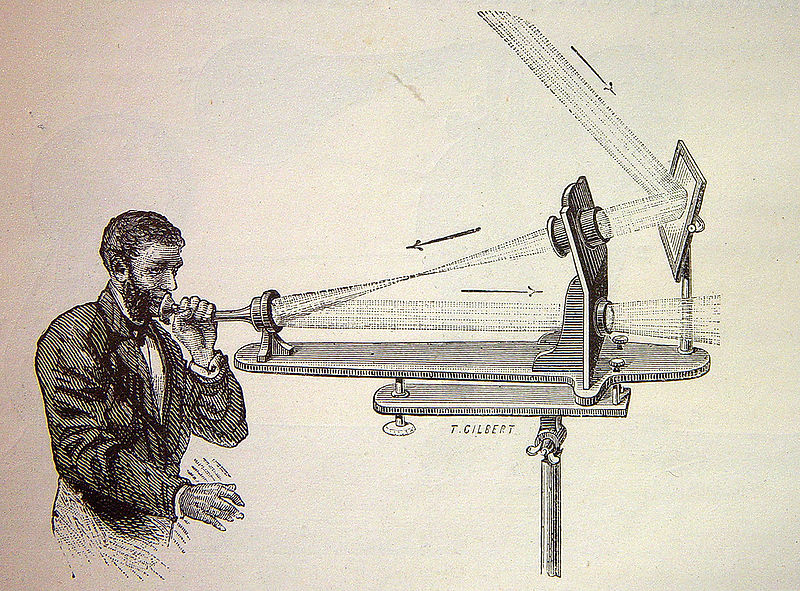
\includegraphics[angle=0,width=\figwidth]{./Figures/Photophone_transmitter.jpg}
\caption[Photophone transmitter]{Graham Bell's photophone transmitter. Sun light modulated with flexible mirror\cite{photoTx}}
%\floatfoot{Source: \url{http://en.wikipedia.org/wiki/File:Photophone_transmitter_4074931746_9f996df841_b.jpg}}
\label{fig:photophone_transmitter}
\end{figure}

%-----------------------------------------------
%\begin{figure}[h]
%%\centering
%\begin{minipage}{.6\textwidth}
%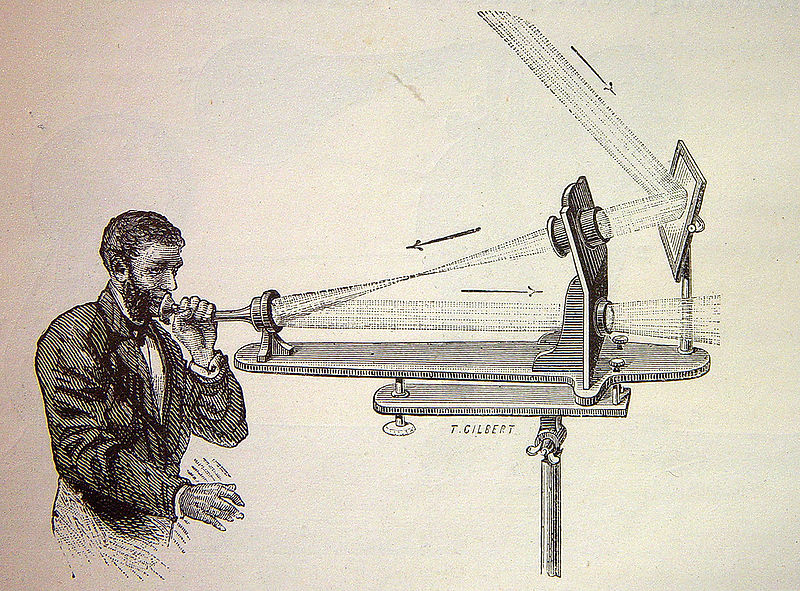
\includegraphics[height=2.9\figheight]{./Figures/Photophone_transmitter.jpg}
%\caption{Lorem}
%\end{minipage}
%\begin{minipage}{.2\textwidth}
%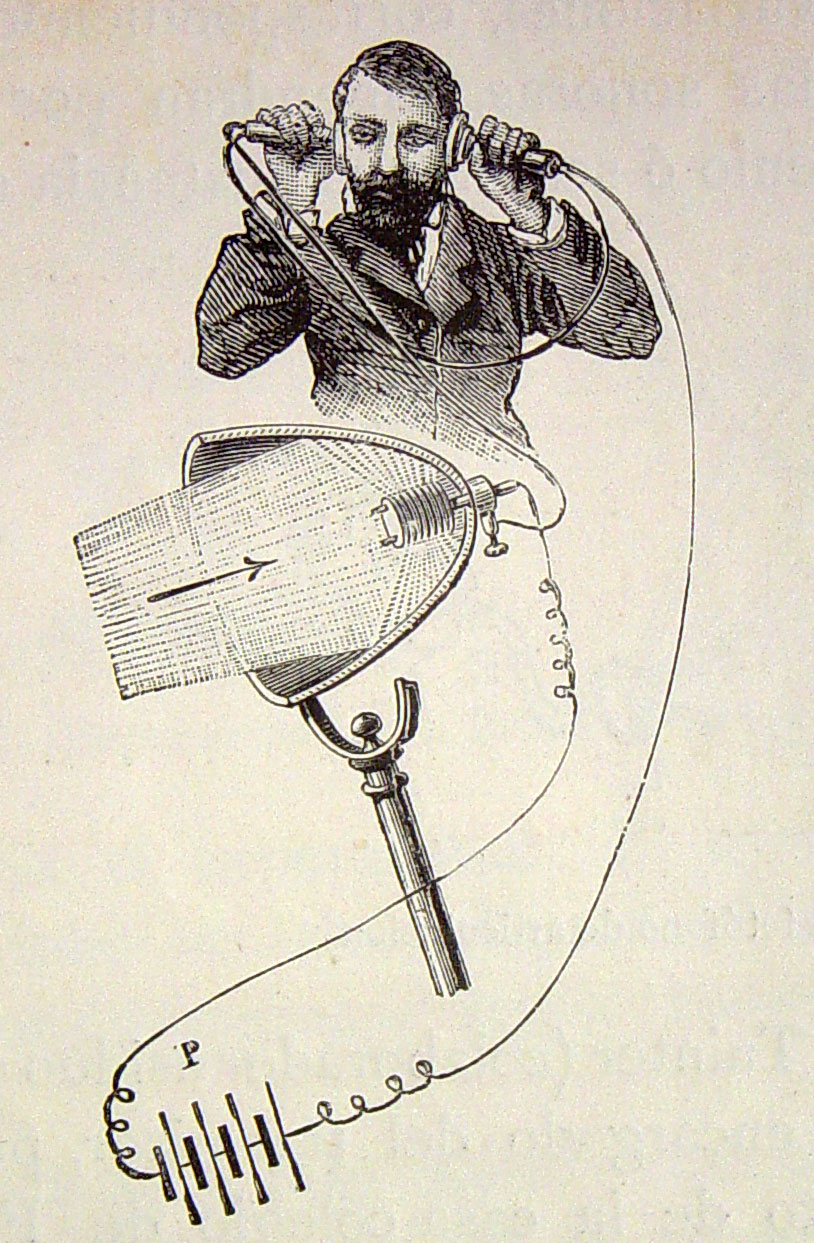
\includegraphics[height=2.9\figheight]{./Figures/Photophone_receiver.jpg}
%\caption{Ipsum}
%\end{minipage}
%\end{figure}
%-----------------------------------------------
%
The receiver consisted of a simpler circuit. It used selenium based crystal detector that conducted electricity in inverse proportion to the incident light. The detector thus converted the incident voice modulated light wave to electric signals. The current passing through detector also energized the speaker coil. The speaker then produced sound according to the current being fed to it. In this way the transmitted voice signal was recovered. The receiver signal is depicted in figure \ref{fig:photophone_receiver}. It is reported that Bell considered photophone his best invention. However it did not enjoy so much popularity as his previous invention of telephone had done. 




\begin{figure}[!hbtp]
\centering
%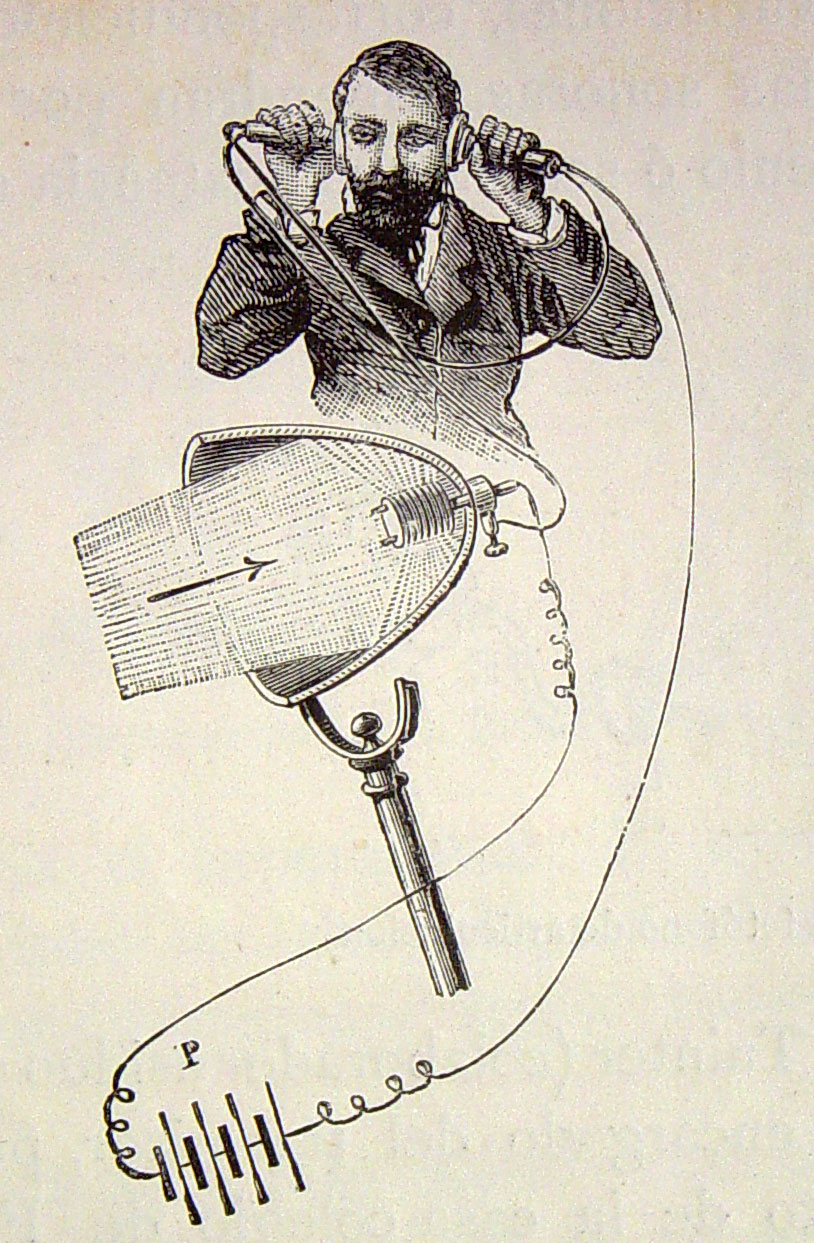
\includegraphics[angle=0,width=\textwidth]{./Figures/Photophone_receiver.jpg}
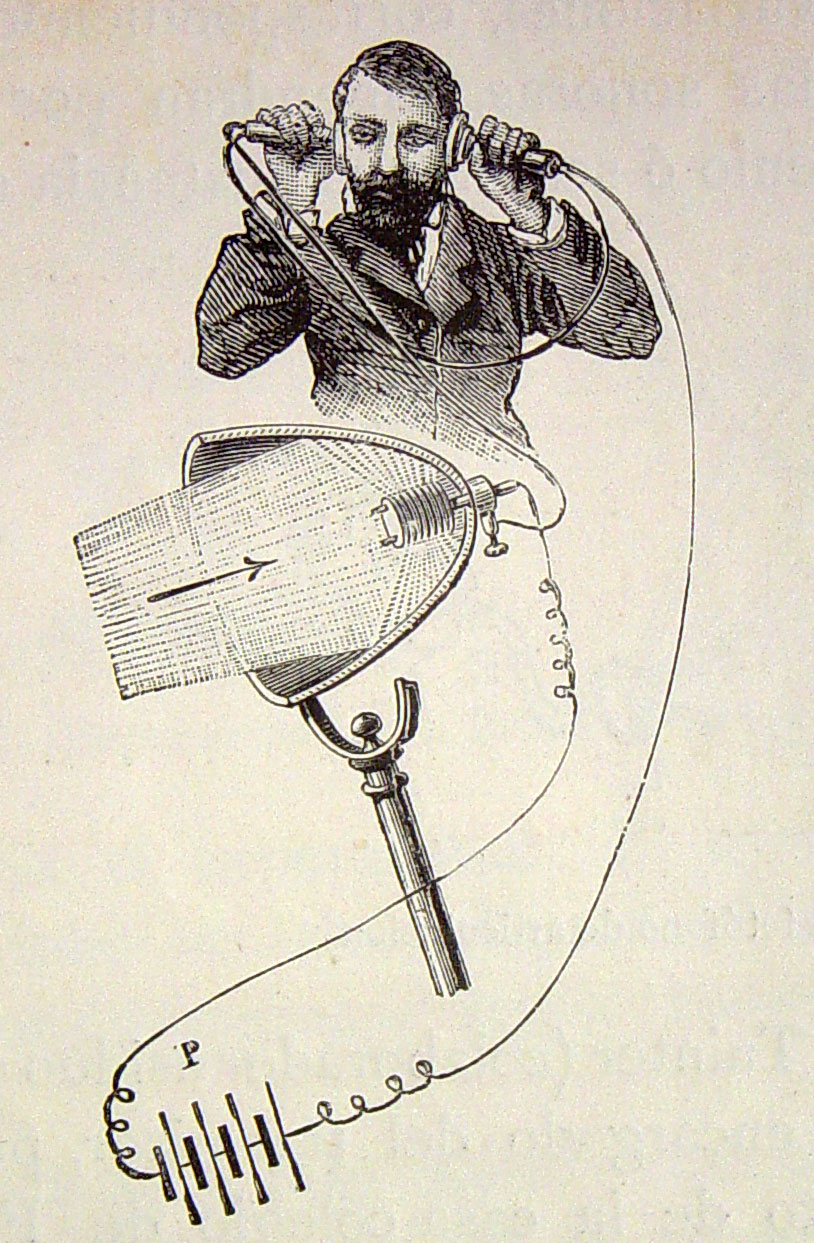
\includegraphics[angle=0,height=7cm]{./Figures/Photophone_receiver.jpg}
\caption[Photophone receiver]{Photophone receiver\cite{photoRx}}
%\floatfoot{Source: \url{http://en.wikipedia.org/wiki/File:Photophone_receiver_4074172975_288f2808f0_o.jpg}}
 \label{fig:photophone_receiver}
\end{figure}
%http://en.wikipedia.org/wiki/File:Photophone_receiver_4074172975_288f2808f0_o.jpg

%-------------------------Complete---------------------------------------------
 

%International consorcium for visibe light communication
%
% What if it could also send streams of data? Traffic lights, television sets, car headlights, billboards and lamps might all suddenly become far more important in our daily lives. We could receive maps from a street light, get news alerts from lamps and download music from electronic posters.


\section{Advantages Of White LEDs Over Conventional Light Sources}



Light emitting diode based solid state lights have gained wide spread popularity in recent years. The active research in high brightness LED electronics has lowered the price with steady improvement in device capabilities. It can be predicted that these solid state devices will be the major illumination source in near future \cite{schubert2005solid}. The LED option is better than conventional filament type Edison light bulbs or gas discharge lamps on several grounds \cite{4781063}. 

%---> Compare LED power efficiency with incadescent and tube lights
%--> Compare LED life expectancy with /////
%\renewcommand{\labelitemi}{$\bullet$}
\begin{list}{$\diamond$}{\setlength{\leftmargin}{.5in}%
\setlength{\rightmargin}{.5in}}

\item Being solid state devices LEDs are capable of switching at frequencies up to several megahertz. This property is very useful to modulate them for high speed data transmission

\item The overall energy efficiency is better than conventional counterparts. An LED can convert up to 80\% of the power intake to the light energy.

\item Light emitting diodes have life expectancy that is several times higher than the competent incandescent type light bulbs, fluorescent tubes and Compact Fluorescent Tubes (CFT).

\item The white light from an RGB (Red-Green-Blue) LED provides control over the hue or light temperature. This feature is quite useful for aesthetics. 

\item Because LEDs are inherently a low voltage and low current device, these can be combined in the form of strings to match for custom voltage and current requirements.

\item LEDs have strong physical structure that makes them suitable in physical vulnerable conditions such as public places or industrial environment.

\item There are lesser environmental hazards associated with the LED lights. Their close counterparts in terms of power efficiency, gas discharge based florescent or compact florescent lamps use mercury that is poisonous to the environment. 

\end{list}

To summarize, LED are a promising choice towards \emph{greener} technology. 

\section{White LED Technology}

White LED are manufactured by using two major distinct device technologies. First one uses the GaInN based blue LED light chip with phosphor encapsulation as shown in figure \ref{fig:phosphor_led}. The blue light emitted from the chip strikes the phosphor that converts the light wavelength from blue to white light. This is the cheaper of the two solution and suffers from two main problems. First of these disadvantages is the requirement of more power as some power is lost in the impact with florescent surface. Secondly the frequency response of phosphor secondary emission is slow that hampers the inherent fast switching characteristics of the LED device.

\begin{figure}[!hbtp]
\centering
%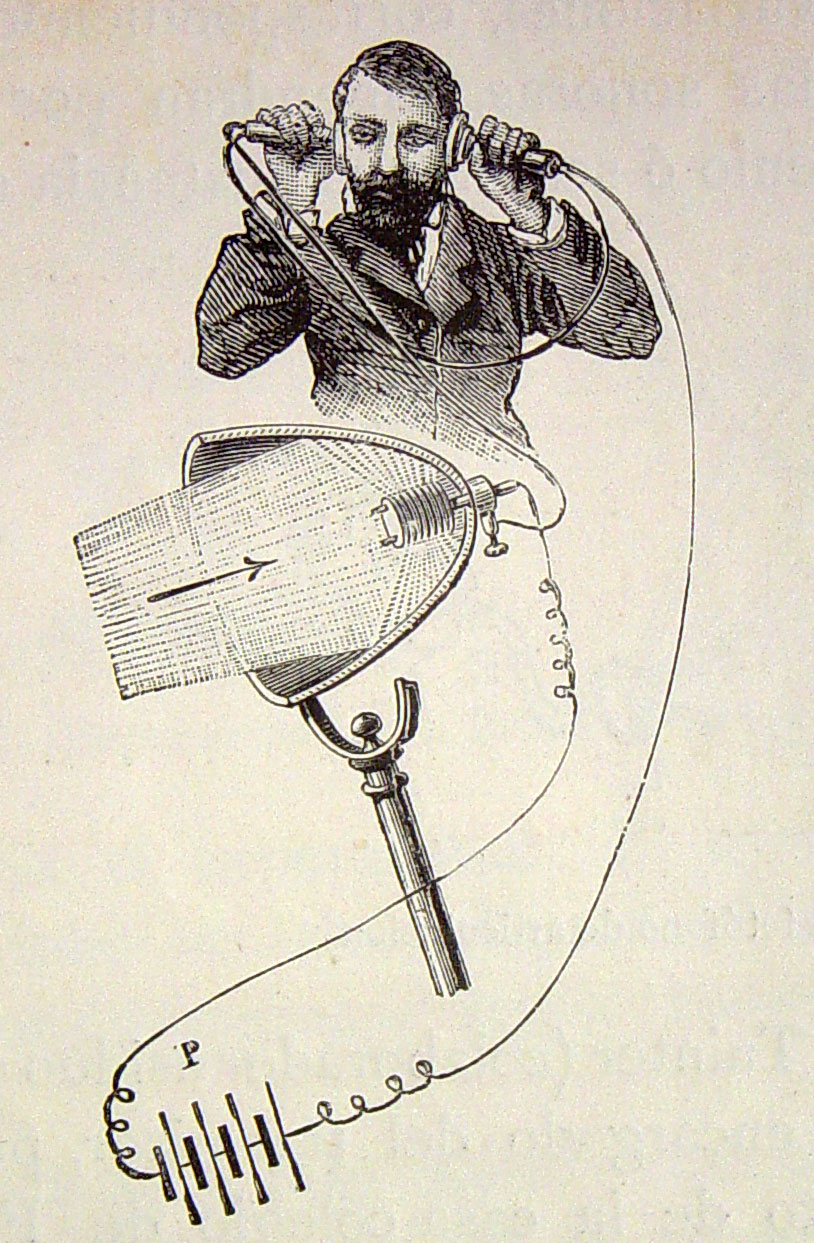
\includegraphics[angle=0,width=\textwidth]{./Figures/Photophone_receiver.jpg}
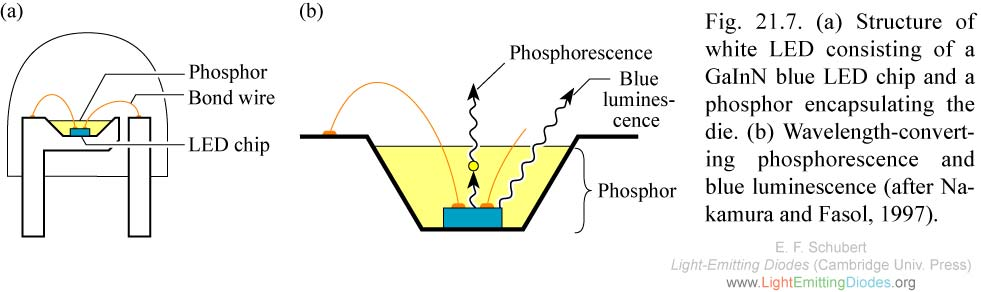
\includegraphics[angle=0,width=\figwidth]{./Figures/slide0011_image007.jpg}
\caption[Structure of a phosphorescence white LED]{Structure of a GaInN phosphorescence based White LED \cite{ledStructure}}%: Image courtesy of E.F Schubert, Cambridge Univ Press, www.LightEmittingDiodes.org }
%\floatfoot{Source: \url{http://www.ecse.rpi.edu/~schubert/Light-Emitting-Diodes-dot-org/chap21/F21-07 Nichia wh LED structu.jpg}}
 \label{fig:phosphor_led}
\end{figure}


The second technology fabricates three devices on a single chip. These devices produce three different colours that are combined to produce white light \ref{fig:RGB_led}. This is the more expensive technology but provides more flexibility in system design. The device has faster switching characteristics than phosphor based LEDs \cite{le2008high} as no second excitation is involved. These devices are also available in packages that have the control pins for the three different colours coming out of the case. These pins can be used to override three different information signals on three available colour wavelengths in a visible light communication scenario. In this way three fold data rate is achieved from a single device using Wavelength Division Multiplexing (WDM). Colour filters are used at the receiver end to separate wavelength multiplexed data streams from original white light.

\begin{figure}[hbtp]
\centering
%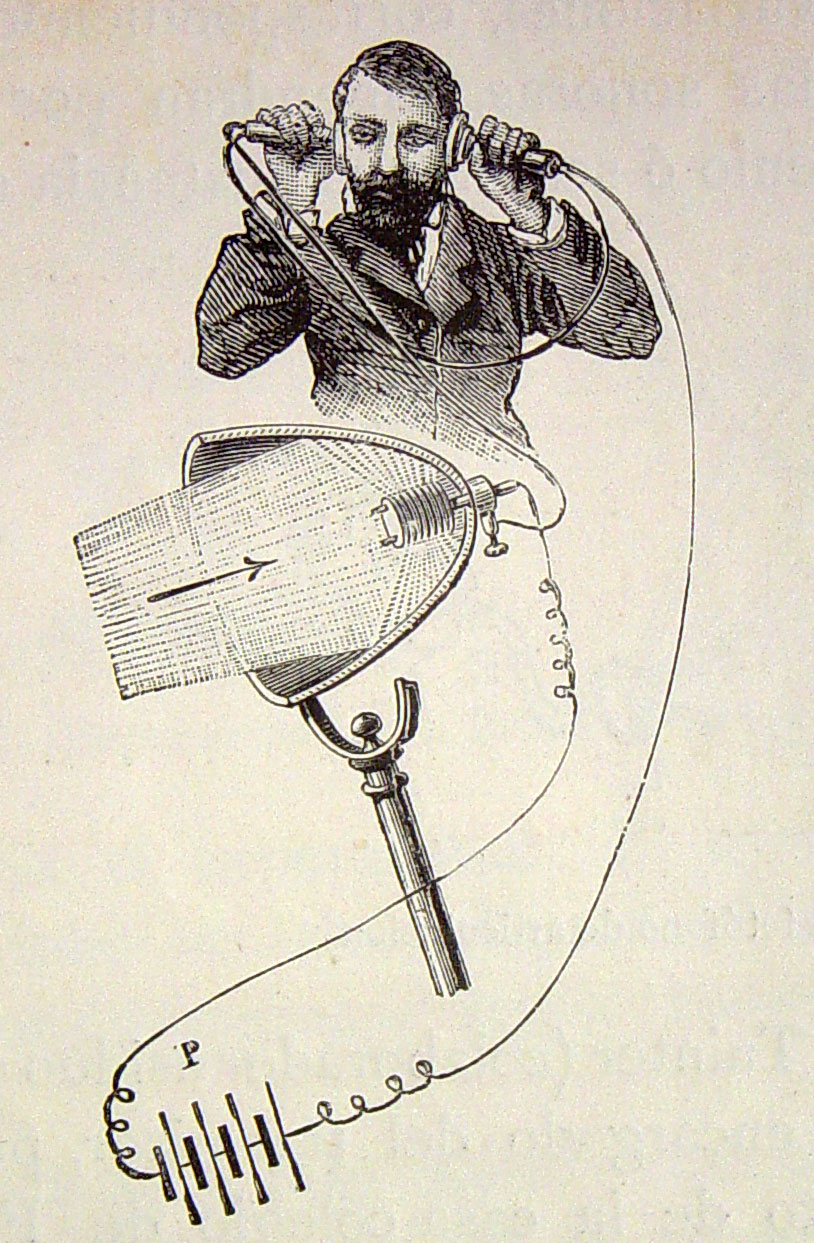
\includegraphics[angle=0,width=\textwidth]{./Figures/Photophone_receiver.jpg}
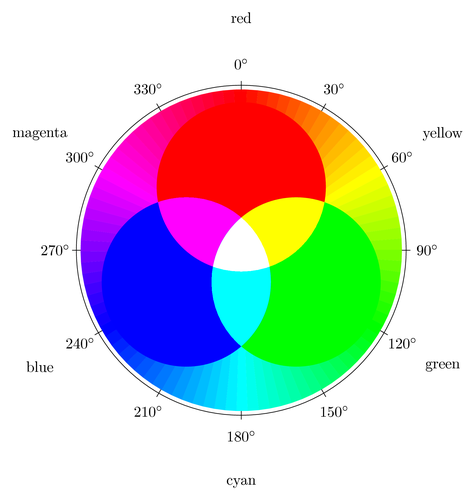
\includegraphics[angle=0,width=.5\textwidth]{./Figures/slide0018_image011.png}
\caption[White light from RGB colours]{White light from intermixing of different wavelengths in an RGB LED \cite{RGBlight}}
%\floatfoot{Source:\url{}}
%\floatfoot{Source: \url{http://media.texample.net/tikz/examples/PNG/rgb-color-mixing.png}}
\label{fig:RGB_led}



%\protect\footnote{and protect my footnotes}
\end{figure}

\section{Visible Light Communication Vs Infrared And Radio Transmission}
Visible light LED based data hotspots have many interesting advantages over other wireless networking technologies such as radio-frequency  and infrared transmission.

\begin{list}{$\ast$}{}
\item Radio spectrum used for wireless communication is getting close to saturation. It is estimated that the consumer bandwidth requirements double every year whereas the technology capacity doubles only in ten years.  Therefore experts are looking for alternate means to fill in this gap. VLC offers a promising new wireless technology with huge bandwidth.

\item Radio spectrum is largely regulated and it is costly to purchase bandwidth. VLC is free from such regulations and therefore it can be readily deployed.

\item There are certain health problems related with high power RF signals \cite{szmigielski1982accelerated} \cite{agarwal2009effects} \cite{wdowiak2007evaluation}. Living cells can be damaged when exposed to power signals for longer time. However there are no such issue with visible light communication.

\item Radio signals interfere with other electronics equipment causing malfunctioning of sensitive devices \cite{robinson1997interference} \cite{van2008electromagnetic}. VLC does not pose such problems which makes it a suitable candidate for access technology in hospital and air planes. 

\item RF equipment is costly and requires extra fixtures for devices. In contrast to that VLC uses the light source for data transmission. Driving the visible light source at high powers is much cheaper. Most of the mobile phones carry flash lights and cameras that have potential to be used as VLC transmitter and receiver respectively. It makes technology adoption at lower cost.

\item It is difficult to confine RF signals within the desired area and faces security risks from eavesdroppers.\cite{racherla2000security}. However visible light is highly directional that reduces the fear of signal capture by wrong recipients. Moreover opaque objects help confine the signal within a closed space. It is an appreciated feature of VLC for security and data privacy.

\item Visible light communication offers superiority over other optical data access technologies like infra-red and ultraviolet transmission. Though in principle it is not different from them, but being visible to eye it fulfils illumination requirements in addition to wireless communication.

\item Because infrared light is invisible, at high power levels it can damage the human eye without being noticed. In VLC's case, human eye closes by reflex action when it senses high powered illumination. That makes the later technology a safer option.

\item Though infrared and ultraviolet lights are directional too, it is somewhat difficult to align the transmitter and receiver because of invisibility of the signal stream. VLC is superior as the illumination can easily be directed to the point where it is required.

\item The information access cum illumination spot can easily be detected by naked eye. This is useful in public data access services. User can spot the places with stronger signal reception. For a comparison this convenience is not available in Wi-Fi systems.


\item Optical transmission is highly directional and needs line of sight signals for effective communication. Here radio transmission wins over VLC.

\item Visible light experiences higher attenuation in atmosphere. Therefore its range is shorter than IR and RF communication.

\end{list}

\section{Where VLC Is Used?}
 LED lights can be designed either to form a focused or a diffused light beam. Former configuration has found applications in point to point communication links.  The focused beam applications include free space optical (FSO) line-of-sight links and optical fibre communication. Though the communication may take place in visible light spectrum in above mentioned technologies, these are not categorized under visible light communication. VLC applies to the scenarios where transmitting light source is not a spacial communication device but rather its primary function is something else, like illumination \cite{komine2004fundamental} or signalling. This thesis focuses on applications where illumination is the main feature of LED light source and it provides ubiquitous communication as an added luxury \cite{VLCC}.

The VLC lights can be deployed indoors or outdoors with pros and cons of each scenario. In indoor environment, receiver gets light not only from direct light of sight but also from secondary reflections by room walls and other objects. In this case it is not all too necessary for transmitter and receiver to be in line of sight. However in outdoor situations this advantage may not exist.

\begin{figure}[hbtp]
\centering
%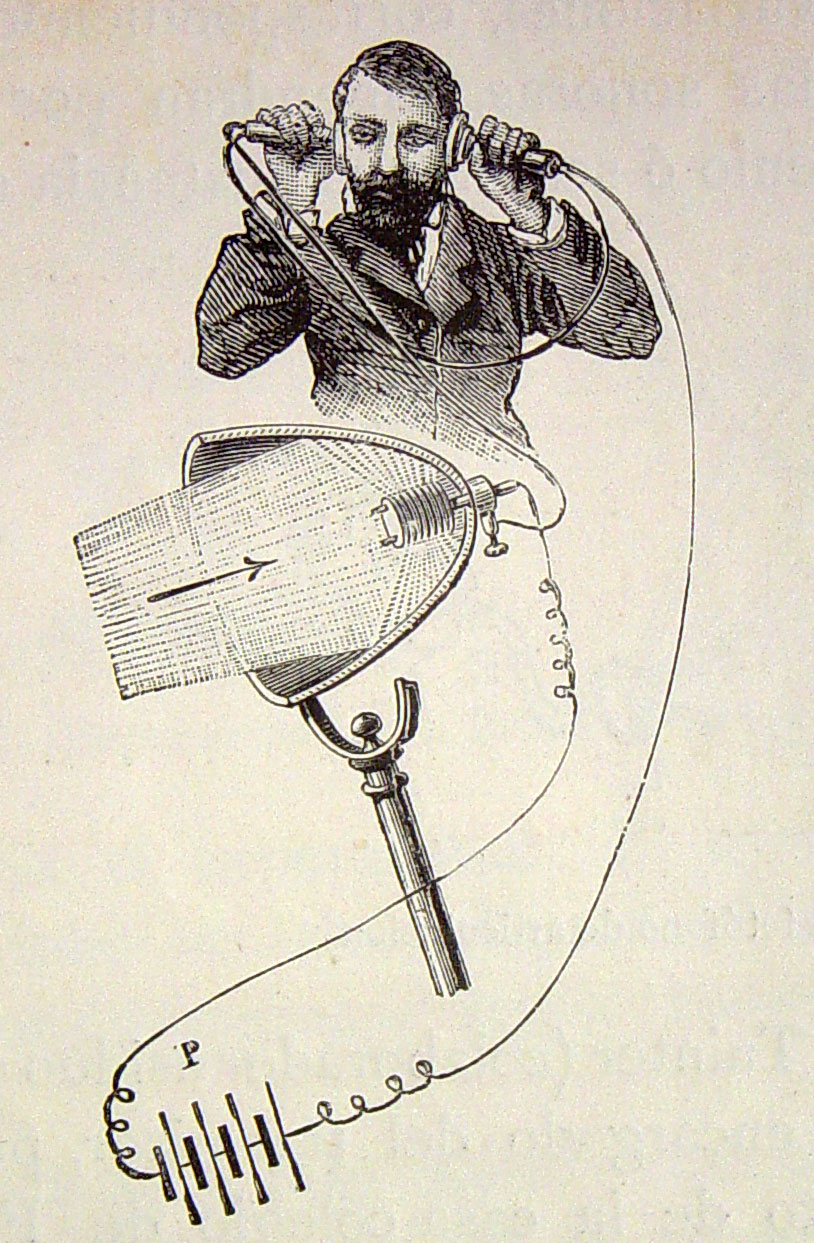
\includegraphics[angle=0,width=\textwidth]{./Figures/Photophone_receiver.jpg}
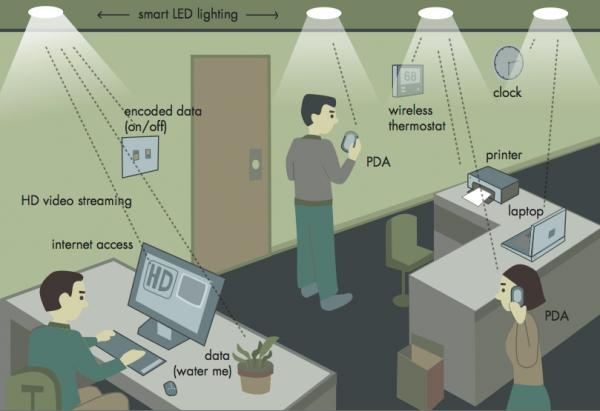
\includegraphics[angle=0,width=.9\textwidth]{./Figures/VLC_Room.jpg}

\caption[Visible light communication in office]{Visible light communication indoor scenario \cite{VLCroom}}
%\floatfoot{Source:\url{	www.eetimes.com/electronics-news/4199568/Visible-light-illuminates-a-new-approach-for-wireless-comms}}
 \label{fig:VLC_room}
\end{figure}

%Photographer's or artist's name (often not given)
%Name of subject or title of picture
%Date of picture (often not given)
%Title of website
%URL
%Date you accessed the picture.

The signals reflected by walls and other objects in indoor environment pose greater intersymbol interference due to multiple delayed versions of the same signal \cite{komine2004fundamental}. It puts a limit on maximum transmission speed. However outdoor lights do not suffer from this limitation. On the other hand outdoor lighting are affected by environmental conditions such as fog, smoke and rapid temperature variations. In indoor environment these conditions are very much under control.

In indoor environment, the positioning systems such as GPS largely fail or provide false reading due to inadequate RF signals \cite{dedes2005indoor}. In one of the VLC applications, light fixture sends information pulses with source position tags. A hand-held receiver device reads these tags from different light sources to estimate its position \cite{tanaka2009new}. This application is useful for sight impaired patients, helping them in navigation through hospitals corridors.

In departmental stores VLC light fixtures can be used to inform customers about different products in their vicinity. A cheap photo sensor mounted on the trolley receives this information and displays it on a small attached LCD screen. Similarly museums can use light sources placed to illuminate objects as well as transmit information about them. A tourist with a cheap hand held device pointed at illuminating LED can hear or read the information he wants without disturbing others. Even mobile phones can be used as the receiving device as cameras can be found on majority of the phones now a days.

A new term Li-Fi has been evolved to describe the wireless networking environment based upon visible light communication, inspired from Wi-Fi. There is research going on for embedding the power line communication (PLC) with VLC for ubiquitous broadband access networked computing \cite{komine2003integrated}.

Another form of VLC is proposed for vehicle to vehicle communication \cite{dunning2004inter}. The tail light of a car ahead communicates with the photosensor mounted on the car following behind. It has potential use as a collision avoidance technology. Another research focuses on data transmission by LED traffic signals to the surrounding vehicles \cite{arai2007experimental} about congestions warnings, alternate routes etc. It may also be possible to get map information from these signals.

Electronic sign boards can also be enabled to transmit data by modulating the light \cite{park2007information}. Similarly television sets, computer screens and back lights of mobile phone displays have been demonstrated to transmit information in the form of visible light. VLC has also found applications in high speed communication in underwater environment where radio signals undergo higher attenuation.
%------------------------ 

To summarize, white LED based lighting cum data transmission solutions can widely be used in home automation, broadcasting at shopping malls, precision indoor positioning and navigational aids, indoor wireless networks in hospitals, aircrafts and spaceships etc.

\section{Thesis Objectives}
The main objective of this thesis is to solve an important problem associated with the drive signal for information carrying light source. Dimming control of the communicating LED lights is an important requirement as lighting is their primary feature. However the information modulation and dimming control signals interfere with each other. Conventionally dual modulation techniques are used to mitigate this interference. We propose a novel line coding scheme, Variable Rate Multipulse Pulse Position Modulation (VR-MPPM), that achieves brightness control as well as data transmission using single modulation signal.

Power spectral density of the proposed encoding scheme is obtained to evaluate the effect of brightness level and brightness resolution on spectral characteristics. The underlying tradeoffs between brightness resolution and successful data transmission rate are evaluated for optimal performance. The proposed scheme is tested on FPGA based hardware setup to evaluate bit error performance at different brightness levels and brightness resolutions.

\section{Research Papers}
As part of this research, a conference paper \cite{siddique2011joint} was submitted to \emph{CCNC'2011 - Smart Spaces and Personal Area Networks}. The paper proposed the VR-MPPM line coding scheme for joint brightness control and data transmission of VLC lights. It presented simple iterative data encoding and decoding algorithms along with practical and numerical evaluation of the proposed scheme.

Another paper has been submitted to \emph{IEEE communications Letters} that analyses the spectral properties of VR-MPPM encoding schemes. The underlying tradeoffs between brightness resolution and symbol error rate are discussed to select optimal symbol frame size.

\section{Organization Of The Thesis}
In order to provide the theoretical background for the research work done in this thesis, the study of existing modulation schemes for joint dimming control and data communication of LED lamps is presented in chapter 2. In Chapter 3 the proposed modulation scheme is developed to jointly achieve brightness control and data transmission for a VLC light source. Simple iterative encoder and decoder algorithms are also developed that are explained with the help of simple examples. Chapter 4 evaluates the spectral properties of the proposed scheme. The spectrum analysis methodology is explained with the help of an example. The effect of symbol frame size and brightness level on power spectrum are evaluated. In Chapter 5, objective function for optimal selection of frame size for minimum symbol error rate and maximum brightness resolution is evaluated. Hardware implementation of the proposed line codes and dependence of symbol error rate on brightness index is  also observed in this part. Finally we draw our conclusions in Chapter 6.

%\section{Research Papers}
%As part of this research, a conference paper \cite{siddique2011joint} has been presented in \emph{CCNC'2011 - Smart Spaces and Personal Area Networks}. The paper proposed the VR-MPPM symbol encoding algorithm along with its practical and numerical evaluations.


%\textbf{Joint Brightness Control and Data Transmission for Visible Light communication Systems based on White LEDs}
%We have submitted another paper to \emph{IEEE communications Letters} that analyses the spectral properties of VR-MPPM encoding schemes. The underlying tradeoffs between brightness resolution and symbol error rate for selection of optimal symbol frame size are also discussed. % Introduction 
%
%% Chapter 2
% add following line for typesetting from subfiles
% !TeX root = ../uet_thesis.tex
% !TeX root = ../uet_thesis.bbl
% !TeX root = ../references.bib

\chapter{Literature Survey} % Write in your own chapter title
\label{Chapter2}
\lhead{Chapter 2. \emph{Literature Survey}} % Write in your own chapter title to set the page header
%\section{Introduction}

%2)	Literature Review
%i)	Brightness control of leds
%(a)	PWM and PAM techniques
%ii)	Optical data transmission techniques
%(a)	PPM, MPPM, VW-MPPM
%iii)	Problem: joint brightness control and data transmission
%(a)	Nakagawa’s Approach



%Komine's fundamental analysis of visible light communication

%Passage from CCNC paper
The dual objectives of brightness control and data transmission for white LED based lighting infrastructures are interrelated but are mostly addressed separately in literature. In situations where LED lights are used for illumination purpose, methodology for dimming control of the light intensity is discussed in isolation, without referring to the visible light communication. In other cases these devices are considered in data communication scenario with little consideration imparted to the brightness control of the transmitting device. However as the visible light communication is concerned about the situations where illumination is the primary functionality and claims as much importance as the data being transmitted, it is necessary for the LED devices in such dual applications to be dimmable according to the user requirements.

The brightness control of LED lights is mostly achieved by using pulse-width-modulation (PWM) \cite{doshi2010control}, \cite{mick2006led} \cite{garcia2009dimming}, that provides control over full brightness range of the device by changing duty cycle of the pulsed drive current. The control over brightness level can also be achieved by controlling amplitude of the drive current, i.e. pulse amplitude modulation (PAM) \cite{fang2009apc}. Both PWM and PAM are analogue techniques by nature. In case of PWM the pulse timing is varied in continuous time while PAM needs continuous variation in the drive current magnitude. Therefore these techniques are not suitable for digital systems. Control of brightness level by controlling the drive current magnitude poses the problem of chromatic shift \cite{dyble2005impact} \cite{levada2006high}. The colour of white LED light varies at different drive current levels. Therefore PWM is preferred over drive current magnitude or PAM based solutions.

On the other hand the modulation techniques employed in optical communication systems have been designed either to improve power efficiency or enhance the bandwidth utilization. Pulse position modulation (PPM) scheme is often employed in infrared communication and free space optical (FSO) links \cite{audeh1996performance} \cite{lesh1983capacity} due to its high power efficiency. Another variant of PPM in the form of differential pulse position modulation (DPPM) is used to serve the same purpose \cite{shiu1999differential} more efficiently. Optical modulation schemes that focus on enhancing bandwidth utilization include multi-pulse pulse position modulation (MPPM) \cite{kozawa2008enhancement}, \cite{xu2009coded}, \cite{sugiyama1989mppm} and dicode pulse position modulation (DPPM) \cite{sibley2003dicode}. The bandwidth utilization is improved by using more than one pulse in a PPM frame, thus giving more combinations of codewords to encode symbols. The other variation of PPM, DPPM, employs multilevel pulses to achieve high data rates. Another interesting modulation technique for indoor infrared wireless communication is presented in \cite{garrido2006variable}. It proposes a rate-adaptive transmission scheme based on MPPM block codes. This technique aims to achieve power  and bandwidth efficiency simultaneously by choosing the codewords selectively. 

The literature referred in preceding paragraphs discusses optical transmission focusing either on optimal bandwidth utilization or improving power efficiency. However no attention has been imparted to the brightness control of the transmitting signal. One reason for this bias comes from the fact that these modulation schemes were originally designed for infrared wireless communication, free space optical (FSO) links or fiber optic link. These scenarios do not pose any special brightness control requirements. Therefore all of the techniques mentioned above fall short of the brightness control mechanism. However this point can not be ignored in case of visible light communication based optical links.

A related work \cite{zeng2007tunable} proposes the pulse amplitude modulation and pulse width modulation in a hybrid mode to maintain good power and bandwidth efficiencies under time varying channel conditions. This scheme has potential to be used as a joint brightness control and data transmission scheme under stable channel conditions.

Techniques to tackle the two issues of brightness control and data transmission simultaneously have just started to emerge. One such technique  purposes the use of sub-carrier pulse position modulation (SC-PPM) as a solution \cite{sugiyama2007brightness}. This SC-PPM sends the PPM pulse in the form of a high frequency carrier. The equivalent PPM slots carrying no pulse are transmitted by an arbitrary constant value. The brightness control is achieved by changing the modulation depth of the sub-carrier as shown in figure \ref{fig:carrier_depth}. The signal levels $a$, $b$ and $c$ allow the source drive signal average value control without effecting the information symbol. On receiver side, this carrier signal is passed through a band pass filter after detection through an optical sensor. This band pass filter is centred at sub-carrier frequency and helps recover original PPM frame. Modulation depth and the slots without pulses grant the signal DC average value to be set anywhere from 0\% to 100\% of maximum signal value. This achieves the control over brightness level independent of the information symbols being transmitted.

\begin{figure}
	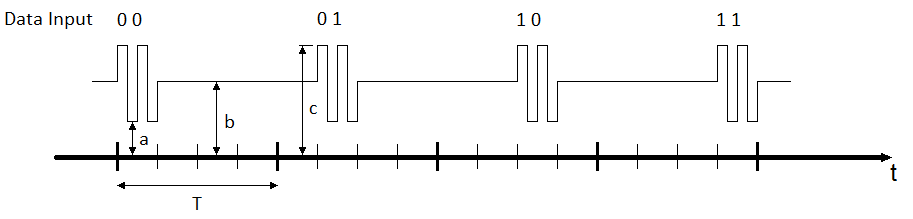
\includegraphics[width=\textwidth]{./Figures/slide0042_image022.png}
	\caption{Brithness control using sub-carrier modulation}
	\label{fig:carrier_depth}
\end{figure}

There is another joint brightness control and data transmission method proposed in the same paper \cite{sugiyama2007brightness}. The second solution employs PWM modulation of sub-carrier to set the average value of SC-PPM drive signal. This approach provides limited brightness control in the range 0\% to 87.5\%. Additional low pass filter is required at receiver end to get rid of the overriding PWM signal in origional PPM pulsed slots.

Both of the discussed solutions have their shortcomings in digital systems due to use of much higher frequency switching pulses for sub-carrier while actual data transmission rate is low. Moreover the modulation control circuitry is based upon analogue hardware that tends to be expensive and less power efficient. On the positive side, presence of sub-carrier provides better noise immunity to external noises such as florescent tube lights flickering as such disturbances are filtered out by the bandpass filter on receiver side.  However there is an associated deficit that much of the device bandwidth is lost to the high frequency carrier. Therefore these schemes are useful only for low speed data transmission.

A recent research \cite{bai2010joint} proposes the use of overlapping pulse position modulation (OPPM) for simultaneous brightness control and data transmission.  OPPM allows the pulses in adjacent slots to overlap. The constant duty cycle signal is then amplitude modulated to achieve brightness control. This scheme, too, achieves brightness control through drive current intensity control that renders it not so preferred solution for digital systems.

%One more publication \cite{sugiyama2006experimental} considers both the communication and brightness aspects of led lights, proposes methods such as inverted pulse position modulation and subcarrier inverted pulse position modulation to achieve the two objectives simultaneously. However it emphasises more on rejecting the background light flickering noise.

 % What to Write 
%
%% Chapter 3
% add following line for typesetting from subfiles
% !TeX root = ../uet_thesis.tex
% !TeX root = ../uet_thesis.bbl
% !TeX root = ../references.bib
\chapter{Proposed Solution} % Write in your own chapter title
\label{Chapter3}
\lhead{Chapter 3. \emph{Proposed Solution}} % Write in your own chapter title to set the page header
%\section{Introduction}

%3)	Proposed Solution: Joint Brightness control and data transmission
%i)	PPM extension to multipulse block
%(a)	Combinatorial studies of MPPM
%ii)	MPPM for joint brightness control
%(a)	MPPM line codes for a simple case
%Algorithm for Implementation of MPPM code
%iii)	Decoder Algorithm
%(a)	Flow graph
%(b)	Matlab implementation
%(c)	Decoding example for case (5,2)
%iv)	Encoder Algorithm 
%(a)	Flow graph
%(b)	Matlab implementation

%(c)	Decoding example for case (5,2)

The requirement of joint brightness control and data transmission is met by proposing a novel line coding scheme. The proposed scheme does not require conventional dual modulation schemes based solution to meet the two objectives. The single modulation scheme pulse width modulates (PWM) the LED light source for brightness level and transmits data symbols at the same time with these PWM pulses. No additional analogue hardware is required. Simple iterative algorithms encodes and decodes the line coded symbols in linear time complexity. These algorithms are explained with examples. In following lines we start to solve the original problem from perspective of conventional line coding schemes, explaining the gradual development of proposed scheme.

\section{On-Off Keying In Visible Light Communication (VLC)}
%Before discussing the proposed scheme it would be useful to go through conventional line coding schemes in visible light communication scenario.
The simplest modulation technique for data transmission over optical networks is on-off-keying (OOK) that transmits data by turning the signal on for the signal bit \emph{one} and turning it off for signal bit \emph{zero}. This scheme can not be used to drive optical signal in visible light communication scenario because OOK does not possess a constant duty cycle (DC) or average value. Rather its DC average is a function of information bits statistics, how these are appearing in the signal. A light modulated with OOK will have flickering effect due to uneven distribution of ones and zeros. Besides that there is no way to control the brightness level. To understand this just imagine what happens when there is a long stream of ones, the light is illuminated to full brightness long as long as these ones keep on repeating. On the other hand when there is a long stream of zeros, light is essentially turned off. For any other random distribution of ones and zeros light intensity keeps on fluctuating in proportion to their presence in the data stream. Thus it is evident that OOK is not a proper solution to transmit data when illumination is the primary function of the light source.
%insert figure of an OOK driving signal here.

The light flickering problem can be cured by utilizing a constant average value line code such as  Manchester coding. In this case the light source intensity would remain constant for human eye perception, provided that the bit frequency is chosen high enough. To control the brightness level drive signal can be overridden by a DC offset signal. Though the brightness level can be set in this solution, however it is not a preferred scheme in 'all digital' system concept as it calls upon analogue hardware. It is also lesser power efficient and poses risk of LED chromatic shift \cite{dyble2005impact} \cite{levada2006high}. We are still seeking for a solution that has brightness control built in the encoding scheme itself.

\section{Pulse Position Modulation (PPM) \& VLC}
Another popular line coding technique for transmission over optical networks is pulse position modulation (PPM). It transmits data in the form of information blocks or frames. A PPM block consists of fixed number of time slots per frame, $n$, one of which contains a pulse and the rest remain at zero level. The position of the pulse within the frame determines the value of information to be transmitted. A 4-slot PPM frame can transmit a pulse in any one of the four possible slot positions. It provides four different combinations for a single 4-PPM frame. A combination denotes an information symbols. It means that the 4-PPM frame can transmit two information bits per frame. PPM is in fact a block coding scheme. A block code translate a group of input bits to a group of output bits. These two bit groups are called as information symbol $s_k$ and the encoded symbol $s_n$.
 %insert figure for PPM frame% 

\begin{figure}[t]
\centering
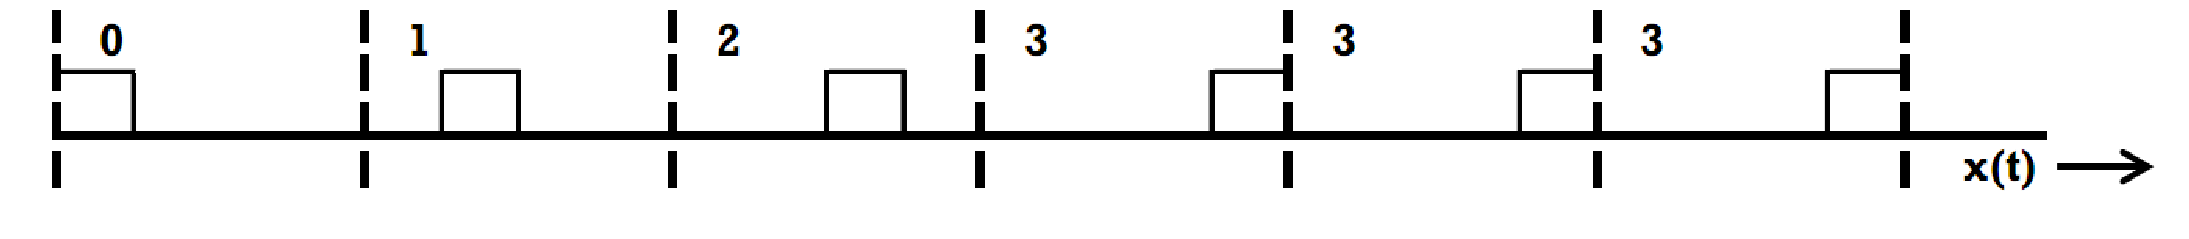
\includegraphics[width = \figwidth]{../Figures/PPM_frame}
\caption[PPM Signal]{A PPM signal transmits information symbols by position of the pulse in the frame. Digits 0,1,2 and 3 represent the information symbol being encoded.}
\label{fig:PPM_frame}
\end{figure}




A close inspection of PPM signal reveals that the average value of this signal remains fixed irrespective of the statistics of input bits. For a 4-PPM case, signal average value remains fixed at 25\% of the peak value at all times. To summarize above discussion, PPM is a constant average value or constant duty cycle (DC) technique that promises fixed illumination for the transmitting terminal light. In this way by employing PPM technique the flicker problem is solved. However the second problem of achieving control over brightness level remains unsolved. It is required that this DC average should be changeable without requiring external analogue hardware and without disturbing the data transmission.


%Heading PPM used for brightness control
%inser picture that shows PPM with 2,4 and 8 slot frames for brightness control
 This is an interesting question and to answer it we revisit the PPM encoding scheme. As noted above, average value of a PPM signal is $\frac{1}{frame~size}$. It shows the signal average value is inversely proportional to the frame size. That means the light source brightness can be changed by changing the frame size. For example if the 4-PPM is changed to 2-PPM, signal average value is doubled from quarter of the maximum voltage to the half of the maximum voltage level. Accordingly the information carrying capacity of a frame will be halved too, from 2-bits per frame to now only 1-bit per frame. Similarly by expanding the frame size from 4-PPM to 8-PPM, signal intensity would by halved from quarter of maximum to one eighth of the maximum drive voltage. The effect on information carrying capacity would be increase in bits per frame to 3-bits per frame. Though it is an effective technique that serves both the requirement of a modern LED based light source, that is the dimming control and the data transmission from a single line coding scheme. However even this scheme suffers from a few drawbacks. One, the frame size is not constant but is rather a function of brightness requirement of the light source. To decrease the brightness level, frame size must be increased and vice versa. It makes transmitter-receiver synchronization difficult once the brightness level is shifted to some other value. To comply with current industry standards the frame time should remain constant under all conditions. The second problem is that the coderate $\frac{1}{n}\lfloor \log_2(n) \rfloor$ drops with increase in frame size, $n$. Maximum code rate would be achieved for 2-PPM and then it is just half, i.e. one information bit transmitted for two bits of the line coded signal. For other brightness levels, frame size would have to be increased that will further deteriorate the coderate. Thirdly, brightness control is achieved in a non-linear fashion in steps of$\{\frac{1}{2}, \frac{1}{3}, \frac{1}{4}, \cdots \}$. Linear distribution of brightness levels would offer a better control. This discussion incites to search for a still better approach to the problem.

\section{Proposed Variable-Rate Pulse Position Modulation}
%Second thoughts to PPM
To look for a better encoding scheme we revisit the PPM and block codes. Consider all the $n^2$ codes that can be established by an n-bit block code. For didactic reason the example of $n=4$ is chosen. There are sixteen different possible four bit code words possible. These sixteen words can be grouped according to the number of \emph{ones} in a code word. In the described case of $n=4$ there can be total of five groups where each member of a certain group consists of either 0,1,2,3 or 4 ones. The codes in a group share a common property that the code duty cycle or average value is constant. It means if the light source is being modulated with one of the groups its light will remain fixed at one level associated with that group. By modulating with a different group of code words, brightness level can be shifted at the DC value of that very group. For the 4-bit code example, codes 0011 0110 1100 0101 1010 1001 are members of a group that all have 50\% duty cycle. If the group is changed to 0001, 0010, 01000, 1000 the brightness level will be 25\%.  Similarly by using other groups the brightness level can be set at at 0\%, 25\%, 50\%, 75\% or 100\%.  The code grouping according to the brightness levels is shown in table \ref{Ta:code_groupings}. The corresponding light source driving signal waveform is shown in figure \ref{Fig:line_codes}

\begin{table}
\begin{center}
\caption{4-Bit Codeword grouping according to brightness level.}
\begin{tabular}{|c|c|c|c|}
\hline\hline
Output Codeword&Input Symbol&Ones per Codeword& Brightness index\\
 &  $S_k$ & r &  $B_I$ \\
\hline\hline
0000 & 0 (00) & 0 & 0 \\ \hline
0001 & 0 (00) & 1 & 0.25 \\	
0010 & 1 (01) & 1 & 0.25 \\	
0100 & 2 (10) & 1 & 0.25 \\	
1000 & 3 (11) & 1 & 0.25 \\ \hline
0011 & 0 (00) & 2 & 0.5 \\	
0101 & 1 (01) & 2 & 0.5 \\	
0110 & 2 (10) & 2 & 0.5 \\	
1001 & 3 (11) & 2 & 0.5 \\	
1010 & 4 (100) & 2 & 0.5 \\	
1100 & 5 (101) & 2 & 0.5 \\ \hline
0111 & 0 (00) & 3 & 0.75 \\	
1011 & 1 (01) & 3 & 0.75 \\	
1101 & 2 (10) & 3 & 0.75 \\	
1110 & 3 (11) & 3 & 0.75 \\ \hline
1111 & 0 (00) & 4 & 1 \\ \hline
\hline
\end{tabular}
\label{Ta:code_groupings}
\end{center}
\end{table}


\begin{figure}[!htbp]
\centering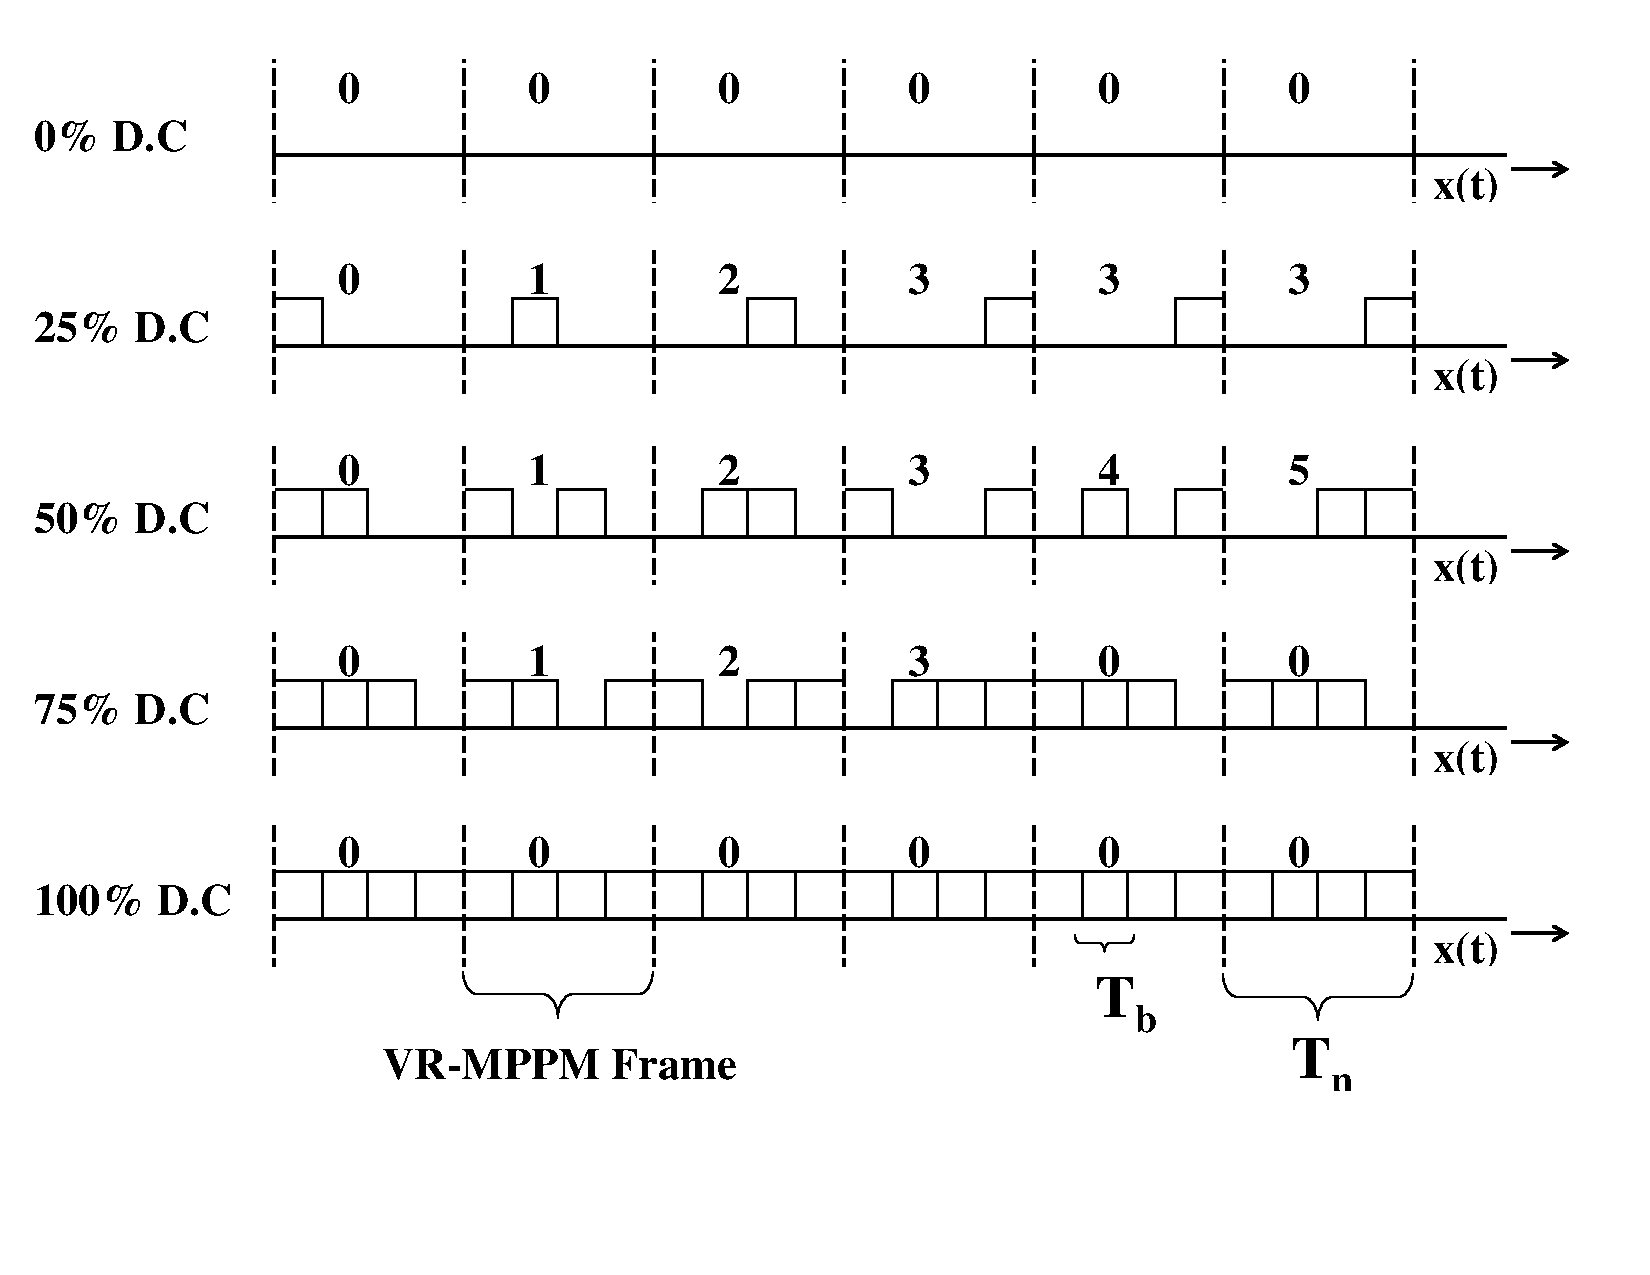
\includegraphics[width=\textwidth]{./Figures/line_code}
\caption{VR-MPPM encoded waveforms at different brightness indices }
\label{Fig:line_codes}
\end{figure}
%insert figure n=4 all possible codes 2^n 
%inser table (optional) with codes with number of ones and the brightness level
%insert waveform showing modulator output waveform

This is the solution presented in this thesis to achieve joint brightness control and data transmission of LED based light source. In above discussion, though the codes for 0\% and 100\% are valid as for as brightness control is concerned, however no information transmission is possible for these two cases. The former case (i.e. code 0000) applies to the situation when the light source is completely turned off and the later (code 1111) applies to the situation when light is fully turned on and there is no switching what so ever in the driving signal. From above discussion it can be inferred that the number of possible brightness levels with $n-bit$ codeword is $n+1$. The brightness level is identified by the number of 1's in a codeword that will now be represented by the variable $r$ such that $r \in \{0,1,2,\cdots,n-1,n\}$. An $n-bit$ long code word group with $r$ number of ones will be represented by symbol $(n,r)$. It represents that there are $r$ ones and $n-r$ zeros in the codeword. Here a new parameter \emph{Brightness Index} can be defined as:

\[\text{Brightness Index   } B_I = \frac{r}{n}\]
\begin{equation}
\begin{array}{cccl}

Where&&& \\
&r&=&\text{number of ones per codeword}\\
&n&=&\text{code word size}\\
	\end{array} 
\end{equation}

The value of brightness index takes values between zero and one with the two extremes being the case for light turned off and light turned on at full brightness when $r$ varied. By setting $n$ a fixed value as a system design parameter, a brightness control cum data transmission scheme evolves that has fixed frame size.


There is a relationship as how many different codewords are possible with a particular selection of $r$ at some fixed value of $n$. In fact this is similar to the classical problem of picking $r$ objects from $n$ total objects. The total number of combinations in this can be calculated by the combinational formula in equation \ref{eq:cominations}.

\begin{equation}
^nC_r = \frac{n!}{r! (n-r)!}
\label{eq:cominations}
\end{equation}•

The more combinations for a particular selection of $r$ the more number of information bits can be transmitted per frame size $n$. However the possible symbols from above formula do not necessarily form a fixed bit value. For instance the $n=4$ case discussed above does produce 4 different combinations for each value of $r=1$ and $r=3$. That can decode two information bits per symbol. However, for the case of $r=2$ there are six different possible symbols.  The effective bits that can be transmitted is still two. To transmitted three bits there must have been eight different symbols. Thus the effective number of transmitted bits per code word is calculated by equation \ref{eq:bits_per_codeword}:
\begin{equation}
Bits~per~codeword = \lfloor \log_2(^nC_r) \rfloor
\label{eq:bits_per_codeword}
\end{equation}•

Taking floor function means that some of the codewords need to be discarded. These extra codewords can be used for signalling information, such as receiver transmitter synchronization. 

Code rate for block codes is defined as the information bits transmitted per codeword bit. An $n$ bit long codeword with $r$ ones transmits at an effective code rate of $\frac{1}{n}\lfloor \log_2(^nC_r) \rfloor$. 

The proposed scheme can be thought as a variat of pulse position modulation that uses multiple pulses per frame instead of just one pulse. For this reason this coding scheme has been named as \emph{Variable Rate Multipulse Pulse Position Modulation (VR-MPPM)}. The acronym VR reminds that the code rate is not the constant but varies according to the selected brightness level.

The $2^n$ output symbols space is distributed among different brightness groups according to the following equation.
\[ 2^n=\binom{n}{0}+\binom{n}{1}+\underbrace{\cdots+ \binom{n}{r} +\cdots}_\text{r$\rightarrow$ 1's, (n-r)$\rightarrow$ 0's}+\binom{n}{n} \]

Though the assignment of input bit symbol to $2^n$ output codeword in table \ref{Ta:code_groupings} seems arbitrary at first glance, a novel algorithm has been designed in this thesis that performs this mapping in linear time complexity. This algorithm is explained in following passages.

\section{Algorithm}
The format of encoded word is similar in principle to the digit place value weightage function used in decimal and binary systems. Binary system assign place value to digits as $1,2,4,8,\cdots,so~on$ starting with least significant digit value equal to one. Similarly the decimal system assigns $1,10,100,1000,\cdot,~so~on$ as digit place values. However the proposed scheme has a small difference from these systems in that the place value for a digit is not fixed. Like binary system the digits used are 0's and 1's only. 

The place value system for a codeword of size $n$ with $r$ ones is discussed here. The weightage function is assigned to a \emph{digit} in the codeword as $\binom{i}{\rho}$, where $i$ and $\rho$ are two variables that index the digit in the code-word. The variable $i \in \{ 0,1,2,\cdots,n-1\}$ indexes the absolute  position of the digit in the codeword, zero being the index number for least significant digit. The variable $\rho \in \{1,2,\cdots,r\}$ indexes only the 1's in the codeword. The two possible values of $r = 0$ and $r = n$, though form valid codewords, are not considered here as these correspond to the two extreme conditions of light fully turned off or fully turned on and the communication is not possible in these cases. Thus for algorithm's purpose the values of $r$ is restricted to $r \in \{1,2,3,\cdots,n-1 \}$

%starting at 3:37 19-oct-2011
An information symbol $s_k \in \{0,1,2,\cdots,\lfloor \log_2(^nC_r) \rfloor \}$ encoded with n-bit long word with r-ones is represented by the trio $(n,r,s_k)$. As the code will be used to drive a line signal, the resulting wave form will have $r$ pulsed slots and $n-r$ non pulsed slots in a VR-MPPM frame. To encode the symbol $(n,r,s_k)$ the table \ref{tab:encode-decode} needs to be constructed. This table will be used to lookup the place value of the codeword digits. Each column represents the place value of a digit at index $i$. Each row modifies this place value depending upon the number of pulsed slots in the codeword. An entry $(i,r)$ in the table is constructed according to the relation:
\begin{equation}
\label{eq:placeValue}
    (i,\rho) = \left\{\begin{array}{cc}
    ^{i}C_\rho & i \geq \rho \\
	0 & i < \rho
\end{array}   \right.
\end{equation}

\begin{table*}[t]
\centering \caption{Symbol encoding and decoding matrix}
\begin{tabular}{c|c c c c c c c c} \hline \hline
$\rho \diagdown i$ & ${n-1}$ & ${n-2}$ & $\cdots$ & ${i}$& $\cdots$ & ${2}$ & ${1}$ & ${0}$ \\ \hline \hline
$n-1$ & $^{n-1}C_{n-1}$ & 0 & $\cdots$ & 0 & $\cdots$ & 0 & 0 & 0 \\ 
$n-2$ & $^{n-1}C_{n-2}$ & $^{n-2}C_{n-2}$ & $\cdots$ & 0 & $\cdots$ & 0 & 0 & 0 \\ 
\vspace{-6pt} \\
$\vdots$ & $\vdots$ & $\vdots$ & $\cdots$ & $\vdots$ & $\cdots$ & $\vdots$ & $\vdots$ & $\vdots$ \\ 
\vspace{-6pt} \\
$\rho$ & $^{n-1}C_{\rho}$ & $^{n-2}C_{\rho}$ & $\cdots$ & $^{i}C_{\rho}$ & $\cdots$ & 0 & 0 & 0 \\ 
$\vdots$ & $\vdots$ & $\vdots$ & $\cdots$ & $\vdots$ & $\cdots$ & $\vdots$ & $\vdots$ & $\vdots$ \\ 
\vspace{-6pt} \\
$2$ & $^{n-1}C_{2}$ & $^{n-2}C_{2}$ & $\cdots$ & $^{i}C_{2}$ & $\cdots$ & $^{2}C_{2}$ & 0 & 0 \\
%\vspace{-6pt} \\
$1$ & $^{n-1}C_{1}$ & $^{n-2}C_{1}$ & $\cdots$ & $^{i}C_{1}$ & $\cdots$ & $^{2}C_{1}$ & $^{1}C_{1}$ & 0 \\
\hline 
\end{tabular}
\label{tab:encode-decode}
\end{table*}

\subsection{A Symbol Encoding Example}
It would be easier to explain the code with the help of an example. Let us suppose that the symbols are being encoded to VR-MPPM with frame size of six time slots. Therefore the table \ref{tab:encode-decode} is evaluated for $n=6$ that results in table \ref{tab:encodeMatrix}. When the encoder is set to brightness index of $\frac{4}{6}$, to encode the symbol $s_k=11$ the codeword will be represented by the trio $(n,r,s_k)=(6,4,11)$. Because there are six bits in a codeword, a total of six comparisons will be done to set each bit value. Variable $i$ will be decremented after each comparison while the variable $\rho$ is decremented only if the comparison is successful. The corresponding output codeword bit is set to $\mathbf{1}$ for the latter case.


\begin{table}[!htbp]
\centering \caption{Evaluation of Symbol Encoding Matrix for $n=6$}
\begin{tabular}{|c|llllll|} \hline \hline
$\rho \diagdown i$ & 5 & 4 & 3 & 2 & 1 & 0 \\  \hline \hline
$5$ & 1 & 0 & 0 & 0 & 0 & 0 \\   \hline
$4$ & 5$_{(s_k=11)}$ & 1 & 0 & 0 & 0 & 0 \\   \hline
$3$ & 10 & 4$_{(s_k=6)}$ & 1 & 0 & 0 & 0 \\   \hline
$2$ & 10 & 6 & 3$_{(s_k=2)}$ & 1$_{(s_k=2)}$ & 0 & 0 \\   \hline
$1$ & 5 & 4 & 3 & 2 & 1$_{(s_k=1)}$ & 0 \\   \hline
$0$ & 1 & 1 & 1 & 1 & 1 & 1$_{(s_k=0)}$ \\  \hline \hline
Output Codeword & 1 & 1 & 0 & 1 & 1 & 0 \\  \hline
\end{tabular}
\label{tab:encodeMatrix}
\end{table}


\begin{list}{}{}
\item The encoding process is started at the intersection of column corresponding to $i=5$ and $\rho=4$ which gives a place value of 5 in table \ref{tab:encodeMatrix}. Since this value is smaller than the symbol value $s_k=11$, we set the most significant bit (MSB) to one and subtract the place value from the symbol to get new $s_k=6$. 

\item For next comparison the variable $n$ is decremented. Because the result of last comparison was true, the variable $\rho$ is decremented as well. The place value from table \ref{tab:encodeMatrix} against $i=4$ and $\rho=3$ comes out to be 4. Because $s_k=6$ is greater than 4, the value of $s_k$ is decremented by 4 and the second MSB is also set.

\item The next comparison takes place for $i=3~and~\rho=2$. However this time the symbol value $s_k=2$ is less than the place value 3, the comparison fails. Corresponding codeword is set to zero and comparison is made in next slot.

\item The variable i is decremented from 3 to $i=2$, but the value of $\rho=2$ remains the same. This gives the place value of 1 from  \ref{tab:encodeMatrix}. As $s_k=2$ is greater than one, $s_k,i~and~\rho$  all get decremented accordingly. Codeword bit is set to one.

\item The next comparison is made for $s_k=1,i=1,\rho=1$. The place value of 1 is equal to the symbol value that shows the comparison is successful. The symbol value $s_k$ after decrementing by place value is reduced to zero. 

\item Next the place value is looked in last column at last row where it is 1. Here place value is greater than the symbol value that fails the comparison. Now representing each successful comparison by a bit value of 1 and each failed comparison a value of zero, the code word for $(6,4,11)$ is evaluated to be $[1 1 0 1 1 0]$.

\end{list}

The same procedure has been shown in table \ref{tab:encodeExample}. Reading the table from left to right evaluates the code from most significant binary digit to the least significant digit.
%8:30 am 19 oct to 11:30
\begin{table}[!htbp]
%\centering 
\caption{Symbol encoding illustration}
\begin{tabular}{|r||c|c|c|c|c|c|} 
\hline
$i$ & 5 & 4 & 3 & 2 & 1 & 0 \\  \hline
$\rho$ & 4 & 3 & 2 & 2 & 1 & 0 \\  \hline
$^iC_{\rho}$ & $^5C_4=5$ & $^4C_3=4$ & $^3C_2=3$ & $^2C_2=1$ & $^1C_1=1$ & $^0C_0=1$ \\  \hline
$S_k$ & 11 & 6 & 2 & 2 & 1 & 0 \\  \hline
Conditional & $11\geq5? Y$ & $6\geq4? Y$ & $2\geq3? N$ & $2\geq1? Y$ & $1\geq1? Y$ & $0\geq1? N$ \\  \hline
Code Word & 1 & 1 & 0 & 1 & 1 & 0 \\  \hline
Place Value & 5 & 4 & 0 & 1 & 1 & 0 \\  \hline
\end{tabular}
\label{tab:encodeExample}
\end{table}

%A flow graph implementation of the encoder is shown in figure \ref{fig:encoder}
%\begin{figure}[!htbp]%10:00AM 20 Oct 2011
%\centering
%\includegraphics[height =.4\textheight]{../Figures/encoder}
%\caption{The flow graph for encoder implementation}
%\label{fig:encoder}
%\end{figure}
%

\subsection{Example Codeword Decoding}

The decoding of the encoded symbol is straight forward. If the codeword is n-bit long, the individual digits are numbered 0 through $n-1$ starting at least significant digit(LSD). Next the digit having value are numbered 1 through $r$. The symbol value is calculated by assigning each digit a place value according to the equation \ref{eq:placeValue}. 

The decoding process for the codeword $[110110] $ is elaborated in table \ref{tab:decodeExample}. First row shows the codeword digits that needs to be decoded. In second row the variable i indexes the individual code digits. The LSD gets $i=0$ and MSD gets $i=5$. 
In next step (third row) the variable $\rho$ indexes the ones in the codeword. That means whenever a 1 is encountered the value of $\rho$ gets incremented, while moving from LSD to MSD. The next row evaluates the place value of each digit in the codeword. In last row the place values are summed up to give the symbol value of 11. It returns the same symbol back that was used to illustrate the encoding process.

\begin{table}[!htbp]
%\centering 
\caption{Symbol decoding illustration}
\begin{tabular}{|r||c|c|c|c|c|c|} 
\hline

$Code~Word$ & 1 & 1 & 0 & 1 & 1 & 0 \\  \hline
$i$ & 5 & 4 & 3 & 2 & 1 & 0 \\  \hline
$\rho$ & 4 & 3 & 2 & 2 & 1 & 0 \\  \hline
$^iC_\rho$ & $^5C_4=5$ & $^4C_3=4$ & $^3C_2=3$ & $^2C_2=1$ & $^1C_1=1$ & $^0C_0=1$ \\  \hline
$Digit~Value=11$ & 5 & 4 & 0 & 1 & 1 & 0 \\  \hline
\end{tabular}
\label{tab:decodeExample}
\end{table}



%Hence to increase the brightness cotrol frame size needs to be ats large as possible. However the framw size can not be increased with out check as there is an other parameter of concern that affects the code effectiveness if the sizes is increased unchecked. Though a detailed analysis will be presented later, it is the symbol error probability that increases with the frame size for a fixed error probability.

%
%The decoder implementation flow graph is shown in figure \ref{fig:decoder}
%\begin{figure}[!htbp]
%\centering
%\includegraphics[height =.4\textheight]{../Figures/decoder}
%\caption{The flow graph for decoder implementation}
%\label{fig:decoder}
%\end{figure}


The encoder and decoder are implemented in algorithm \ref{algo:Encoder} and algorithm \ref{algo:Decoder}

\begin{algorithm}[ht] 
\caption{Implementation for encoder} 
\label{algo:Encoder}
\KwIn{Variables $n,~r,~s_k$}
\KwOut{Encoded codeword $cw$}

\While{$n > 0$}
{
\eIf{$0 < r < n$ }
{
$y = ^{n-1}C_r$
}{
$y=0$
}

\eIf{$y \leq s_k$}
{
$s_k = s_k - y$ \\
$cw[n] = 1$ \\
$r = r -1$
}{
$cw[n] = 0$
}
$n = n - 1$
}
\end{algorithm}


\begin{algorithm}[ht] 
\caption{Decoder implementation} 
\label{algo:Decoder}
\KwIn{Codeword $cw$ of length $n$, $s_k=0$, $r=1$}
\KwOut{Data symbol $s_k$}
 
\For{$i \leftarrow 1~\KwTo~ n$}
{
\If{$cw[i] == 1$}
{
\If{$i > r$}
{
$s_k = s_k + ^{i-1}C_r$ 
}
$r = r + 1$
}
}
\end{algorithm}


 % Experimental Setup
%
%% Chapter 4
% add following line for typesetting from subfiles
% !TeX root = ../uet_thesis.tex
% !TeX root = ../uet_thesis.bbl
% !TeX root = ../references.bib
\chapter{Power Spectral Density Analysis of Proposed VR-MPPM} % Write in your own chapter title
\label{Chapter4}
\lhead{Chapter 4. \emph{Power Spectral Density Analysis}} % Write in your own chapter title to set the page header
%\section{Introduction}


%
%4)	PSD Analysis of proposed code
%i)	Method for PSD analysis
%(a)	Spectra Calculation by 1)Bosik 2) Cariolaro: 
%(b)	Ergodicity and wide sense stationarity
%b)	Statelessness of VR-MPPM: Simplifies PSD Analysis
%i)	Equations simplification for MPPM case
%(a)	PSD analysis of a simple case (n=4, BI=.25,  = .25)
%ii)	Implementation
%(a)	MPPM PSD cases: graphs
%(b)	Matlab code
%iii)	PSD Observations
%(a)	Strong spectral component at bit frequency: clock extraction
%(b)	DC component verifies intuition

Power spectral density (PSD) analysis of a signal provides important information about the signal characteristics that help in optimal system design. For that reason the power spectral density analysis of the proposed VR-MPPM encoded signal is being presented here.

Spectral characteristics of a signal determine to a large extent the system complexity. Parameters like bandwidth requirements, presence of adequate frequency components for clock extraction and absence of DC null determine the effectiveness and feasibility of a line code.

Generally codes with smaller bandwidth requirements are preferred over the ones that need larger bandwidth. It is also a desired feature for a line code to have strong spectral component at clock frequency for transmitter-receiver synchronization. Digital line coding schemes like Manchester and Bipolar encoding were designed especially with that purpose in mind. PSD analysis of the proposed VR-MPPM would determine whether or not it is a self clocking code. DC null is a preferred feature in digital signalling. A DC biased signal tends to saturate the capacitive and inductive couplings in the system which preform best with AC signals. Therefore a strong DC bias creates problems in signal reconstruction at digital line repeaters and regenerators along the transmission. In optical transmission networks this requirement can be somewhat relaxed as optical signal is DC signal by its very nature. Optical receivers operate on photon counting principle for pulse detection in this DC biased signal. This is one of the reasons for widespread use of PPM and its variants in optical transmission. The proposed VR-MPPM scheme possesses a strong DC component at all code rates and it determines the brightness level of the visible light communication transmitter. In optical broadcasting systems, such as visible light communication, the need for signal regeneration is not that much of an importance as transmitter and receiver operated in close vicinity. It means that the requirement of DC null for the line code needs to be relaxed in our case.

PPM transmits information by position of a pulse in the symbol frame. Therefore DC average of  the signal remains constant, irrespective of the information bits being transmitted. Same is the case for VR-MPPM encoding with a small difference that DC bias remains constant for a selected brightness level but changes when the brightness level is changed to a new value according to the illumination needs. In a practical situation the requirement of brightness change is not so frequent and may need to be changed after time periods much more longer than the symbol time. Therefore to evaluate the spectral properties of proposed codes it is supposed that the transmitter is set at a certain brightness level that remains constant over infinite time to fulfil  theoretical requirement. The spectral density would be calculated for a fixed frame size and at a particular brightness level.

\section{Signal Stationarity}

The data transmitted by an information source is a random process by its nature. As a result the line code carrying this information is also a random signal. A random process is  categorized as a power signal, that is a signal with finite power.

The proposed VR-MPPM scheme is essentially a blockcode which takes an M-bit input symbol and maps it to a codeword of N bits. This (M,N) block encoder is depicted in figure \ref{block_encoder}. The encoder that performs this mapping is a memoryless system. It means that the encoded output for a symbol remains constant irrespective of its position in the input data stream. Because input bit stream is a random or stochastic process, so is the output signal at encoder output. The statistical properties of the encoder output are function of both the statistical properties of the input symbol sequence and the statistics of the encoder itself. 

\begin{figure}
	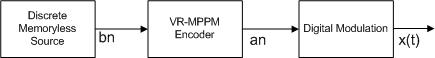
\includegraphics[width=\textwidth]{./Figures/block_encoder}
	\caption{Encoder block diagram}
	\label{block_encoder}
\end{figure}

The PSD of a stochastic process can not be evaluated directly from Fourier Transform due to non-deterministic nature of the signal. In this situation Einstein-Wiener-Khintchine help with a relationship between power spectral density and auto correlation function of a random process, mathematically expressed by equation \ref{eq:wkSx} and equation \ref{eq:wkRx}.

\begin{equation}
	S_x(f)=\int_{-\infty}^{\infty}R_x(\tau)~e^{-j 2 \pi f \tau} d\tau
	\label{eq:wkSx}
\end{equation}

\begin{equation}
	R_x(\tau)=\int_{-\infty}^{\infty}S_x(f)~e^{j 2 \pi f \tau} df
	\label{eq:wkRx}
\end{equation}

The equation \ref{eq:wkSx} possesses special importance as it allows to evaluate PSD of a signal from its autocorrelation function $R_x$. The necessary condition for this relationship to be useful is that the signal should be stationary. That is its statistical properties should not change over time. For communication signals it is enough if the signal meets the two wide sense stationarity criterion given in equations \ref{eq:cond1} and \ref{R_x_t1_t2}.

\begin{equation}
	E\{X(t)\}=\mu_x = Constant
	\label{eq:cond1}
\end{equation}

Where $E\{\cdot\}$ is the expectation operator and $X(t)$ is the random variable for the stochastic process. This equation expresses that the signal mean value should remain constant over time.

\begin{equation}
	R_x(t_1,t_2)=R_x(t_1-t_2)
	\label{eq:cond2}
\end{equation}

The equation \ref{eq:cond2} states that the autocorrelation function should be a function of only the time difference and should not be dependant on absolute time. Therefore $t_1-t_2$ in \ref{eq:cond2} may be replaced by $\tau$, giving $R_x(\tau)=R_x(t_1-t_2)$. It can be evaluated as:

\begin{equation}
	R_x(\tau)=E\{X(t) X(t+\tau)\}
	\label{R_x_t1_t2}
\end{equation}

In our case it is a reasonable assumption that the information source transmits all symbols with equal probabilities and these probabilities do not change over time. It implies that the signal mean and autocorrelation function remain constant with time shift. This satisfies the above mentioned signal widesense stationarity criterion. Since the encoder simply translates input symbols to output codes without memory, encoder output code word sequence also constitute a widesense stationary process. However the encoder output bit sequence is a cyclostationary process \cite{cariolaro1974spectra} with period $N\cdot T_b$, where $T_b$ is the bit period and $N$ is the number of bits per codeword.
%

\section{Spectral Density Formula}
Power spectral density analysis of block coded signals is investigated by several authors. The technique proposed by \cite{cariolaro1974spectra} is the one that will be used for analysis of VR-MPPM block coded signals. However some simplifications of \cite{cariolaro1974spectra} are required to adopt this technique to our case that are listed in table \ref{tab:simplifications}.

%\begin{table}[hbtp]
\begin{table}[htbp]
\begin{center}
\caption[Assumptions for PSD analysis]{Simplifications from \cite{cariolaro1974spectra} technique for analysis of VR-MPPM block coded signals}
\begin{tabular}{|c|c|}
\hline\hline
General Conditions & Simplification for VR-MPPM\\
\hline\hline
\parbox{2.5in}{
\begin{list}{}{}
\item L-step multilevel line code used to encode symbols 
\item Encoder output is a function of code state and input symbol 
\item	Input symbols arrive with any random probability 
\end{list}
}
 & 
\parbox{2.5in}{
\begin{list}{}{}
\item Binary level line code that with signal level 0 or 1
\item Memoryless system that directly maps input symbols to output codeword
\item   All input symbols are assumed to be equally probable 
\end{list}
}\\
%--&--\\
\hline
\end{tabular}

\label{tab:simplifications}
\end{center}
\end{table}

%        L-step multilevel line code used to encode symbols 
%     Binary level line code that with signal level 0 or 1 \\
%	Encoder output is a function of code state and input symbol 
% Memoryless system that directly maps input symbols to output codeword \\
%	Input symbols arrive with any random probability 
%   All input symbols are equally probable 
%	

%>>>>>>>>>>>>>>>>>>>>>>>>>>>>>>>>>>
%   Letter Freq Analysis
%<<<<<<<<<<<<<<<<<<<<<<<<<<<<<<<<<<
%Generally, each codeword of an encoded message is considered to be a random variable and the resulting sequence of codewords constitute a stochastic process. Statistics of sequence of codewords depend on both the statistics of input symbols as well as on the encoding specifications. 



The spectrum analysis starts from representing the encoded signal waveform by its time domain representation. The modulator output signal consists of a pulse train, with certain pulses grouped in blocks or frames. Often the terms slot and bit will be used interchangeably. A bit is the binary value of a symbol in the encoder output codeword in a frame of $n$ bits. This bit is represented by the symbol $s_i^{(j)}$ so that $i$ indexes the frame in the infinite sequence of codewords and $j$ indexes the individual bit within that frame. These bits are modulated by some form of pulse in the time domain. For its simplicity and easier generation in digital systems, we consider the basic rectangular non-return-to-zero (NRZ) pulse shape $p(t)$ as defined by equation \ref{eq:pulseShape}. 

\begin{equation}
\label{eq:pulseShape}
p(t) = \left\{ \begin{array}{cl}
						1&\frac{-T_b}{2} \leq t \leq \frac{T_b}{2} \\
						0&otherwise
						\end{array}
						\right..
\end{equation}

PSD of this NRZ rectangular pulse is provided by equation \ref{eq:spectrumOfRectPulse}. As this term is multiplied to the continuous and discrete spectral components of the encoder frequency spectrum, it determines the overall envelope. For rectangular pulse the spectrum shape decays with higher frequencies according to the $sinc$ function.

\begin{equation}
\label{eq:spectrumOfRectPulse}
 2 T_b \left[\frac{\sin(2\pi f T_b)}{2\pi f T_b}\right]^2
\end{equation}


The frame time, represented by $T_n$, is defined as $T_n=n\cdot T_b$. The resulting continuous time optical signal is given by equation \ref{eq:xt} 

\begin{equation}
\label{eq:xt}
    x(t) = \sum_{i= - \infty}^{\infty} \sum_{j=1}^n s_i^{(j)} p(t- (j-1)T_b - iT_n)
\end{equation}
The power spectral density $S_x(f)$ of a general linear block code is expressed by the following relation \cite{cariolaro1974spectra}

\begin{equation}
S_x(f) = f_n |P(f)|^2 \left\{  \sum_{k=-\infty}^{\infty} e^{ -j \omega k T_n}~ \mathbf{VR_k V^*} \right\}
\label{eq:spectrum_eq1}
\end{equation}
Where $P(f)$ is the Fourier transform of the pulse shape $p(t)$ used for the line code and $f_n=\frac{1}{T_n}$ is the frame repetition frequency. The vector function $\mathbf{V}$ consisting of exponentials terms defined as:

\begin{equation}
	\mathbf{V}= \left[\mathbf{e}^{j\omega T_b}, \mathbf{e}^{j\omega 2T_b}, \cdots,\mathbf{e}^{j\omega nT_b}\right]
\label{eq:vectorV}
\end{equation}

Its complex conjugate transpose $\mathbf{V^*}$ is given by:
\begin{equation}
	\mathbf{V^*}=
		\left[
		\begin{array}{l}
		\mathbf{e}^{-j\omega T_b} \\
		\mathbf{e}^{-j\omega 2T_b} \\
		\cdots \\
		\mathbf{e}^{-j\omega nT_b}
		\end{array}
		\right]
\end{equation}

The parameter $R_k$ is the code correlation matrix defined by equation \ref{eq:corrCoef}.
\begin{eqnarray} \label{eq:corrCoef}
 R_k &=& 
\begin{array}{lc}
   E[\mathbf{s}_i^{T}, \mathbf{s}_{i+k}]  &  -\infty  < k < \infty
\end{array} \nonumber \\
			&=& \mathbf{S}^T \mathbf{P}_k \mathbf{S}
\end{eqnarray}

Where $E[.]$ is the expectation operator and $\mathbf{S} = [\mathbf{s}_1, \mathbf{s}_2, \cdots, \mathbf{s}_m]$ is the codeword translation matrix.  $\mathbf{P}_k$ is the joint probability matrix between any two codewords $\mathbf{s}_{i}$ and $\mathbf{s}_{i+k}$ that occur in the infinite series of codewords that are set apart by $k$ frames.

\cite{cariolaro1974spectra} has presented another expression for the PSD in terms of continuous and discrete power spectra by equation \ref{eq:spectrum_eq2}. This new form is easier to evaluate on digital computers.

\begin{equation}
    S_x(f) = f_n |P(f)|^2 \left\{X_c(f) + f_n X_d(f) \sum_{k=-\infty}^{\infty} \delta (f - k f_n) \right\}
\label{eq:spectrum_eq2}
\end{equation}

Here $X_c(f)$ is the continuous component of the signal spectrum given by 
\begin{equation} 
\label{eq:contSpec}
    X_c(f) =\mathbf{v} (\mathbf{R}_0 - \mathbf{R}_{\infty}) \mathbf{v}^* + 
					2 Re \{\mathbf{v} \Gamma \mathbf{v}^* \} \\
\end{equation}

The discrete spectral component is calculated as follows
\begin{equation} 
\label{eq:discSpec} 
X_d(f) = \mathbf{v} \mathbf{R}_{\infty} \mathbf{v}^*. 
\end{equation}


In equation \ref{eq:contSpec}  $\mathbf{R}_{\infty}$ is defined as, $\mathbf{R}_{\infty} = \lim_{k \rightarrow \infty} \mathbf{R}_{k}$. The $\Gamma$ is defined by the relation 
\begin{equation}
    \Gamma = \sum_{k=1}^{\infty} \exp(j \omega k T_n) (\mathbf{R}_k - \mathbf{R}_{\infty}).
\end{equation}

Because VR-MPPM transmission proposed in this paper exhibits the memoryless property, it leads to the fact that $\mathbf{R}_k = \mathbf{R}_{\infty},~\forall k$. It results in $\Gamma =0$. This fact has considerably reduced the computational burden for evaluation of the continuous spectral component. 

Now $\mathbf{R_0}$ is the code autocorrelation matrix and it can be evaluated from the symbol probability matrix $\mathbf{P_0}$, calculated as $\mathbf{P_0}=\frac{1}{M}\left[~\mathbf{I}~\right]$, where $M$ is the number of valid codewords, calculated as ${\lfloor \log_{2}(^nC_r) \rfloor}$. Thus $\mathbf{R_0}$ can be evaluated to be $\mathbf{R_0}$ =$\frac{1}{\text{M}} \left[\mathbf{S^T~I~S}\right]$. Here $\mathbf{I}$ is the identity matrix of dimension $M \times M$.

Similarly $\mathbf{R_k}$ can be evaluated using the relation $\mathbf{R_k}$ =$\frac{1}{\text{M}^2}\left[\mathbf{S^T~U~S}\right]$. Where $\mathbf{U}$ is an $M \times M$ dimension unitary matrix, having each of its entry equal to one.

The final simplified formulae for continuous and discrete spectral components look like as follows
\begin{eqnarray} 
	\label{eq:spectrum_cont}
	    X_c(f) &=& \mathbf{VS}^T \left(\frac{1}{M}\mathbf{I} - \frac{1}{M^2}\mathbf{U} \right) \mathbf{SV} \\
	\label{eq:spectrum_disc} 
		X_d(f) &=& \frac{1}{M^2} \mathbf{VS}^T \mathbf{U} \mathbf{SV}^*. 
\end{eqnarray}

\section {PSD Analysis By Example}
The PSD algorithm has $\mathbf{O}(n^2)$ time complexity. As an example the spectrum is evaluated at a single normalized frequency point $\frac{f}{f_b}=0.8$ for codeword length $n=4$ and brightness index $B_I=50\%$ (i.e. $r=2$) . The spectrum values at other points on normalized frequency axis can be calculated following the similar steps. First four of the possible six codewords are selected as valid output symbols. The resulting code translation matrix is given as
\begin{equation}
\mathbf{S}=
	\begin{pmatrix}
	     1&     1&     0&     0 \\
	     1 &    0 &    1 &    0 \\
	     0  &   1  &   1  &   0 \\
	     1   &  0   &  0   &  1
	\end{pmatrix} 
\end{equation}

The transpose of code matrix is straight forward
\begin{equation}
\mathbf{S^T}=
	\begin{pmatrix}
     1 &    1&     0&     1\\
     1  &   0 &    1 &    0\\
     0   &  1  &   1  &   0\\
     0    & 0   &  0   &  1
	\end{pmatrix} \\
\end{equation}

The next step is to calculate the code probabilities. As we assumed that all the codes are equal probable, therefore their probability matrix is readily calculated as
\begin{equation}
\mathbf{P_0}=
	\begin{pmatrix}
	     \frac{1}{4}&0&0&0 \\
	     0&\frac{1}{4}&0&0 \\
	     0&0&\frac{1}{4}&0 \\
	     0&0&0&\frac{1}{4} 
	\end{pmatrix} 
\end{equation}

Next the code autocorrelation matrix is calculated using the relation $\mathbf{R_0=S^T P_0 S }$ and it comes out to be
\begin{equation}
\mathbf{R_0}=
	\begin{pmatrix}
	     \frac{3}{4}&\frac{1}{4}&\frac{1}{4}&\frac{1}{4} \\
	     \frac{1}{4}&\frac{1}{4}&\frac{1}{4}&0 \\
	     \frac{1}{4}&\frac{1}{4}&\frac{1}{2}&0 \\
	     \frac{1}{4}& 0             & 0             &\frac{1}{4}
	\end{pmatrix} \\
\end{equation}

Because the encoder is a stateless system, code probability for two codewords $k$ distance apart in the output stream remains constant irrespective of their position in the stream.  This probability matrix is calculated using $\frac{1}{M^2} \mathbf{S^T U S}$, where $M$ is the total number of codewords, four in this case.
\begin{equation}
\mathbf{P_k}=
	\begin{pmatrix}
	     \frac{1}{16}&\frac{1}{16}&\frac{1}{16}&\frac{1}{16}\\
	     \frac{1}{16}&\frac{1}{16}&\frac{1}{16}&\frac{1}{16}\\
	     \frac{1}{16}&\frac{1}{16}&\frac{1}{16}&\frac{1}{16}\\
	     \frac{1}{16}&\frac{1}{16}&\frac{1}{16}&\frac{1}{16}\\
	\end{pmatrix}
\end{equation}
For ${k}\in \{1,2,3,\cdots,\infty \}$

Next the code crosscorrelation matrix $\mathbf{R_k}$ is calculated using $\mathbf{R_k=S^T P_k S }$ that comes out to be
\begin{equation}
\mathbf{R_k}=
	\begin{pmatrix}
	     \frac{9}{16}&\frac{3}{8}&\frac{3}{8}&\frac{3}{16} \\
	     \frac{3}{8}  &\frac{1}{4}&\frac{1}{4}&\frac{1}{8} \\
	     \frac{3}{8}  &\frac{1}{4}&\frac{1}{4}&\frac{1}{8} \\
	     \frac{3}{16} &\frac{1}{8}&\frac{1}{8}&\frac{1}{16} 
	\end{pmatrix}
\end{equation}

The calculation of signal spectrum at the frequency of interest requires the evaluation of vectors $\mathbf{V}=\left[\mathbf{e}^{j\omega T_b}, \mathbf{e}^{j\omega 2T_b}, \cdots,\mathbf{e}^{j\omega nT_b}\right]$ and its complex conjugate transpose vector $\mathbf{V^*}$. The frequency axis is normalized with bit frequency $f_b$ so that the calculations remain independent of a particular bit frequency. It also makes it easier to view the relative frequency components for signals of different frame sizes. \begin{equation}
	{\frac{f}{f_b}}=
	\begin{pmatrix}
	0.8
	\end{pmatrix}
	\label{eq:freq}
\end{equation}

This results in vector $\mathbf{V}$ evaluated as
\begin{equation}
\mathbf{V}=\left[0.3090-0.9511i, -0.8090-0.5878i, -0.8090+0.5878i, 0.3090+0.9511i \right]
\end{equation}

%\[
%	\mathbf{V}= \left[\mathbf{e}^{j\omega T_b}, \mathbf{e}^{j\omega 2T_b}, \cdots,\mathbf{e}^{j\omega nT_b}\right]
%\]
Its corresponding transpose conjugate $\mathbf{V^*}$ comes to be
\begin{equation}
	\mathbf{V^*}=
		\left[
		\begin{array}{r c l}
   0.3090 &+& 0.9511i \\
  -0.8090 &+& 0.5878i \\
  -0.8090 &-& 0.5878i \\
   0.3090 &-& 0.9511i 
		\end{array}
		\right]
\end{equation}

The continuous spectral component is calculated as
\begin{equation}
	{X_c(0.8f_b)}= 1.0239 + 0.0000i
\end{equation}

The discrete spectral component comes out to be
\begin{equation}
	{X_d(0.8f_b)}= 0.4761 + 0.0000i
\end{equation}

The Fourier transform of rectangular pulse $P(f)$ at this frequency is calculated to be
\begin{equation}
	{P(0.8f_b)}= 0.5728 
\end{equation}

The final spectral absolute value at $\frac{f}{f_b} is calculated to be$
\begin{equation}
	{S_x(0.8 f_b)}= 0.1466
	\label{eq:Sx}
\end{equation}

To evaluate the spectrum at other frequencies, equations \ref{eq:freq} through \ref{eq:Sx} are to be evaluated in the similar manner.
%<<<<<<<<<<<<<<<<<<<<<<<<<<<<<<<<<<

\section {PSD Results Evaluation}

% Calculate p(f) for square wave eq:spectrum_disc
 The power spectral density given by equations \ref{eq:spectrum_eq2}, \ref{eq:spectrum_cont} and \ref{eq:spectrum_disc} is evaluated for VR-MPPM encoded signal. The effect of frame size $n$ and brightness-index $B_I$ on the spectral distribution is obtained. 
Basic non-return-to-zero (NRZ) rectangular pulse shape, defined by equation \ref{eq:pulseShape}, is used to represent the binary digits in the codeword. This pulse shape is selected because of the simplicity with which it can be generated in digital systems without requiring complex pulse shaping circuitry. 
\begin{equation}
	p(t) = \left\{ \begin{array}{cl}
			1&\frac{-T_b}{2} \leq t \leq \frac{T_b}{2} \\
			0&otherwise
			\end{array}
			\right..
\end{equation}


\section{Effect Of Brightness Resolution On PSD}

The frame size of VR-MPPM signal determines the available brightness resolution. Equation \ref{eq:spectrum_eq2} is evaluated for different values of frame size $n$ with brightness level fixed at $25\%$. The resulting power spectral density curves are presented in figure \ref{fig:fix_bi}. The top, middle and centre curves represent PSD for frame sizes $n=8, n=12~and~n=16$ respectively. It can be observed from the graph that significant frequency component is present at bit frequency $f_b$ at all frame sizes. The spectral component at bit frequency is plotted at unit point on normalized frequency axis $\frac{f}{f_b}$. Small spikes can be observed overriding all three curves, most significant for $n=8$. These lines indicate that significant spectral components are available at frame clock frequency $f_n = \frac{f_b}{n}$ and its higher order harmonics. Presence of the spectrum lines at both the bit and frame frequencies indicate that the clock signal is well embedded in the proposed line coding scheme that would be helpful in receiver-transmitter synchronization. 

It can also be observed that improving the brightness resolution, by increasing $n$, also smooths the PSD. Most of the spectrum power lies within the bit frequency and decays sharply beyond that.

 \begin{figure}[!hbtp]
  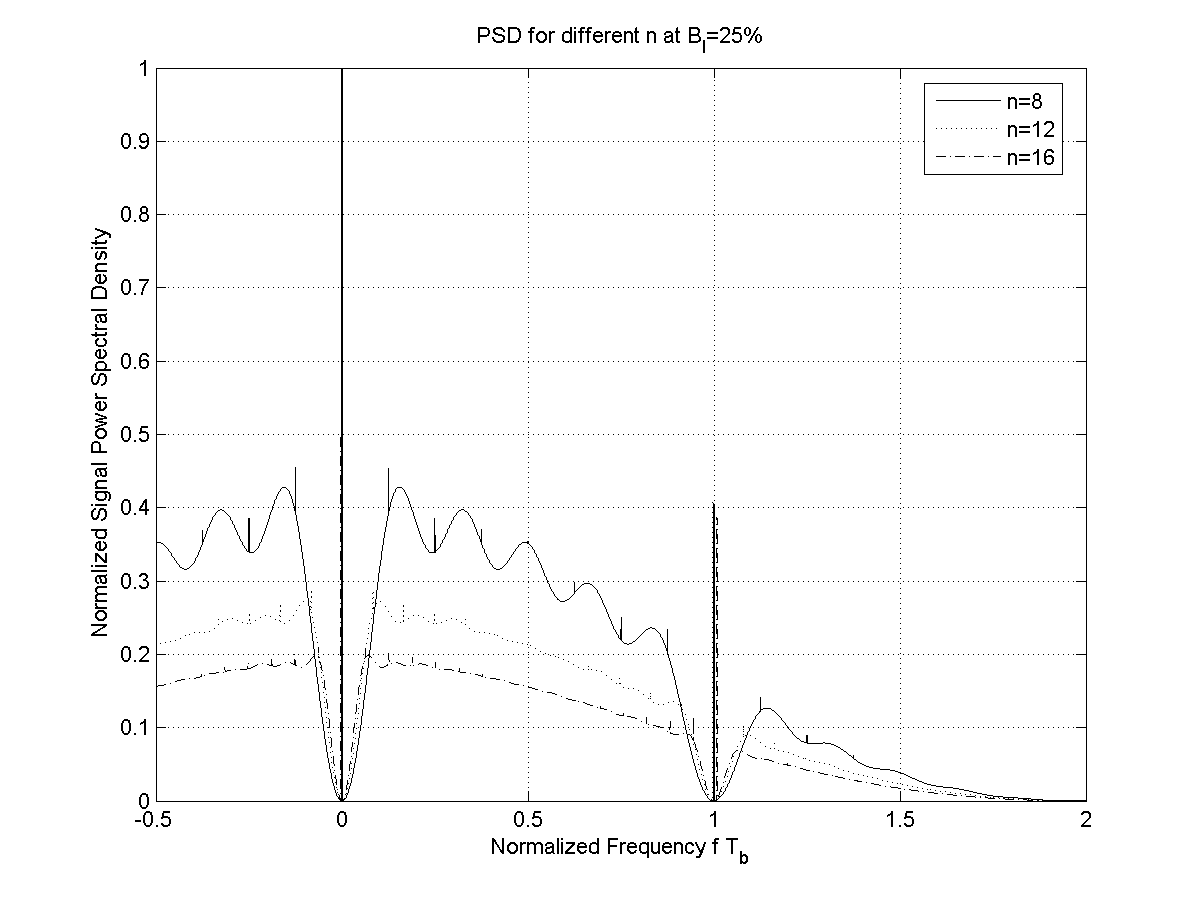
\includegraphics[width=\figwidth]{./Figures/252.png}  
%  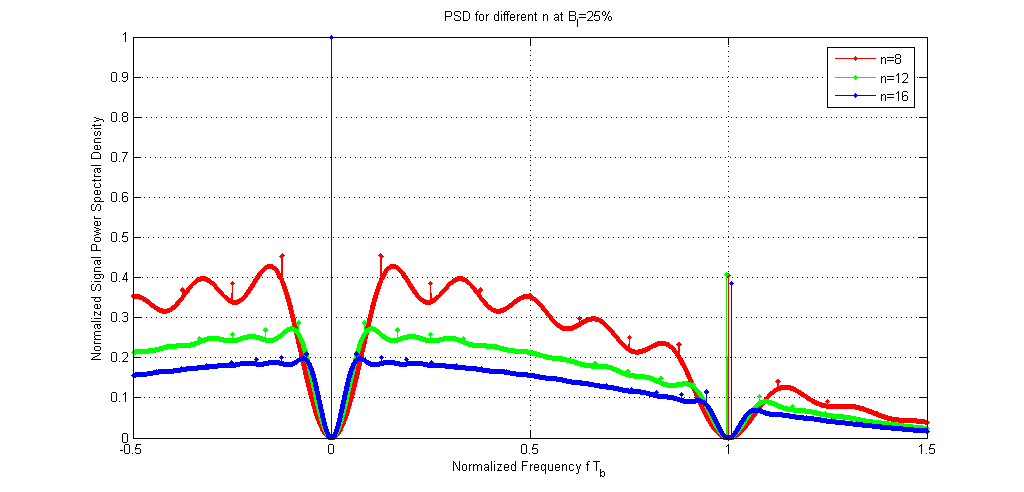
\includegraphics[width=\figwidth]{./Figures/25.png}   Colored Spectrum
  \caption[Effect of frame size on PSD]{Power spectral density for different values of frame size at fixed brightness index}
  \label {fig:fix_bi}
 \end{figure}

%\section{Effect Of Brightness Index $B_I$ On PSD}
\section{Effect Of Brightness Index On PSD}
Effect of brightness index with fixed frame size is plotted in figure \ref{fig:fix_n}. Brightness index has a profound effect on the DC spectral component. The plotted figure shows PSD for $n=8$ at $r=1,2~and~4$ respectively. The inspection of the spectrum at null frequency reveals that when the brightness index is doubled from 0.125 to 0.25,
increase in the corresponding DC component is four fold, from 0.125 to 0.5. Similarly increasing $B_I$ from 0.25 to 0.5, quadruples the DC component form 0.25 to 2.0. This behaviour is expected and confirms the squared relationship between signal voltage and its power. 


 \begin{figure}[hbtp]
  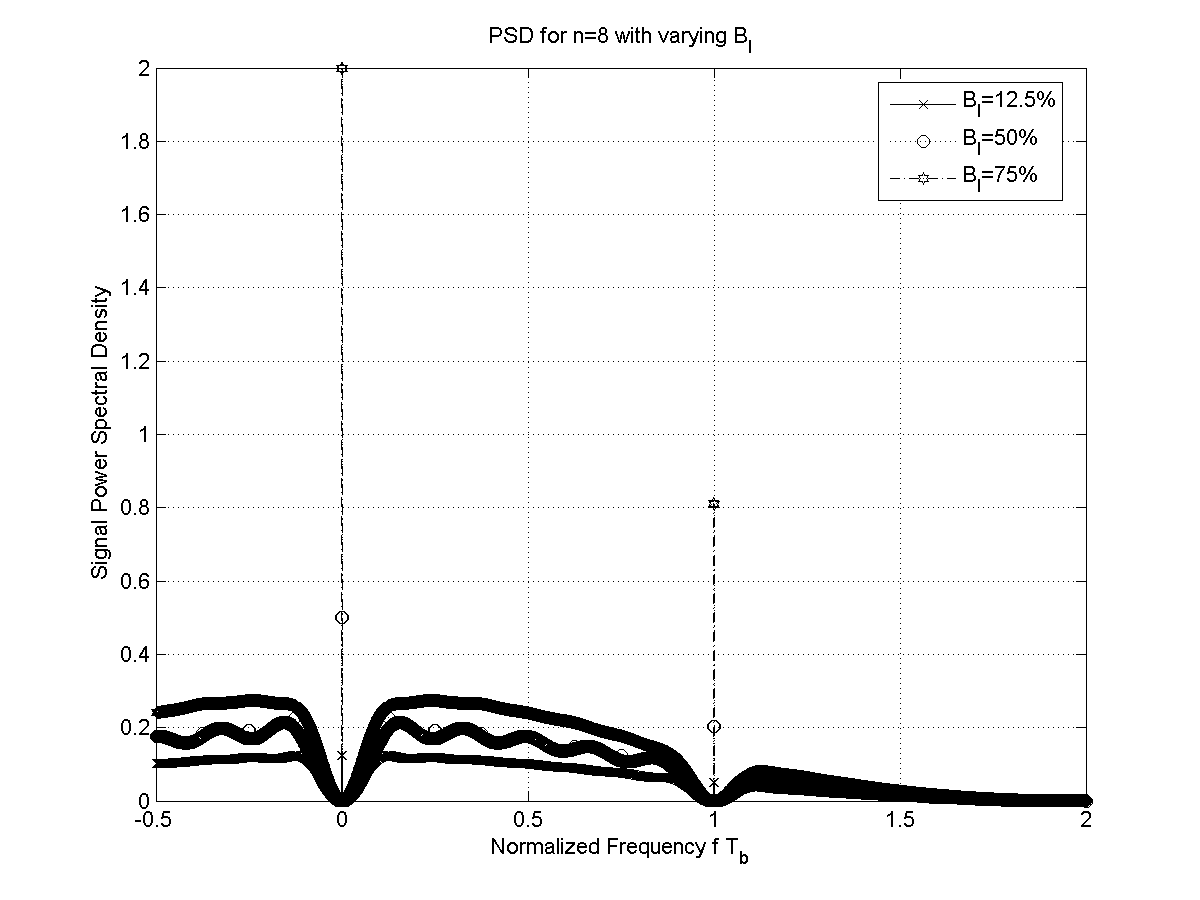
\includegraphics[width=\figwidth]{./Figures/fixN2.png}  
  \caption[Effect of brightness index on PSD]{Effect of changing brightness index on power spectral density, frame size being fixed}
  \label {fig:fix_n}
 \end{figure}

\section{Oscillations In The Spectrum}
%\sloppy
The continuous spectrum displays oscillatory behaviour which is significant at smaller frame size, $n$.  The number of oscillations increases with large codeword size with decreasing magnitude of oscillations. It is due to the influence of vector $V$ defined in (\ref{eq:vectorV}), reproduced below. Figure \ref{fig:OscilationWithN} shows the plot of continuous spectra for n= 2, 4, 8 and 16, evaluated to study the effect of oscillations. Though frame sizes of 2 and 4 provide poor brightness control resolution, the spectrum oscillations are much pronounced here. These graphs are plotted for fixed $r=1$ and PSDs are displaced vertically to separate apart for better inspection. It can be observed that the oscillations diminish for higher values of frame size. This is the same behaviour as adding more exponential terms to Fourier representation of a pulse smothers its time representation towards a better looking rectangle.

\[
	\mathbf{V}= \left[\mathbf{e}^{j\omega T_b}, \mathbf{e}^{j\omega 2T_b}, \cdots,\mathbf{e}^{j\omega nT_b}\right]
\]

 \begin{figure}[!hbtp]
  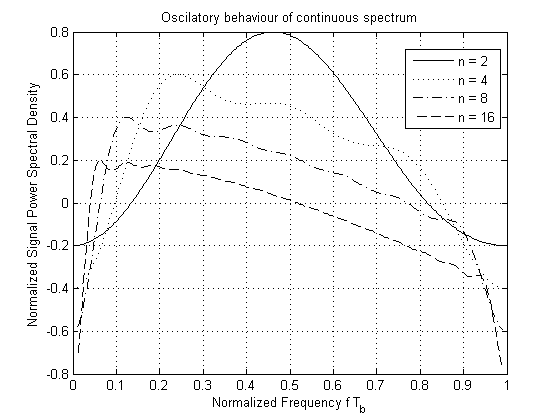
\includegraphics[width=\figwidth]{./Figures/OscilationWithN.png}  
  \caption{Oscillatory trend in spectral density}
  \label {fig:OscilationWithN}
 \end{figure}

The oscillations in continuous spectrum do not change much for a fixed frame size when brightness index is varied. It can be observed from the PSD for $n=10$ at different brightness indices, plotted in figure \ref{fig:OscilationWithR}. 

 \begin{figure}[!hbtp]
  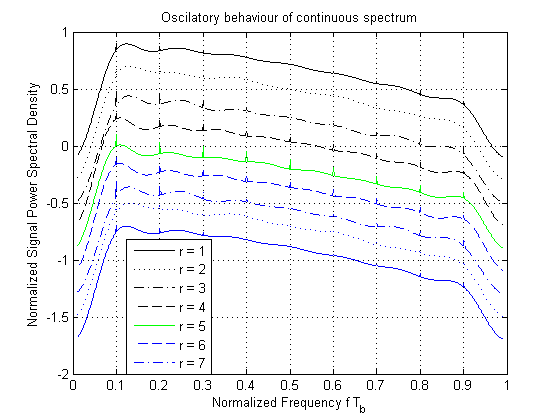
\includegraphics[width=\figwidth]{./Figures/OscilationWithR.png}  
  \caption[Effect of $B_I$ on oscilations in PSD]{Effect of brightness index on oscillations in power spectral density}
  \label {fig:OscilationWithR}
 \end{figure}

%Calculate fn

%>>>>>>>>>>>>>>>>>>>>>>>>>>>>>>>>>>
%
%<<<<<<<<<<<<<<<<<<<<<<<<<<<<<<<<<<

%<<<<<<<<<<<<<<<<<<<<<<<<<<<<<<<<<< % Experiment 1
%
%% Chapter 5
% add following line for typesetting from subfiles
% !TeX root = ../uet_thesis.tex
% !TeX root = ../uet_thesis.bbl
% !TeX root = ../references.bib
\chapter{Performance Optimization} % Write in your own chapter title
\label{Chapter5}
\lhead{Chapter 5. \emph{Performance Optimization}} % Write in your own chapter title to set the page header
%\section{Introduction}


%5)	Implementation and performance evaluation (Hardware + Error Probability)
%i)	Transmitter
%ii)	Receiver
%iii)	Practical results: P_e Vs Brightness Index
%iv)	Maximization Problem

The performance of proposed VR-MPPM codes depends upon several factors like brightness resolution, brightness index and channel conditions. The brightness resolution of VR-MPPM has a direct relation with codeword size. Therefore for better dimming control it is desired that the codeword size should be as large as possible. Information carrying capacity also increases with larger codewords. However there are certain constraints that degrade the line code performance if the codeword size is increased arbitrarily. Numerical performance evaluation results are provided for optimal choice of the symbol codeword size. System design parameters and constraints are formulated as an optimization problem to balance the underlying tradeoffs between brightness resolution and the successful data transmission. 

\section{Effect of Brightness Index and Brightness Resolution on Data Rate}

%As stated above before the information carrying capacity of the proposed codes is affected by the selection of the codeword. A larger code size ensures more brightness levels and better information carrying capacity per symbol frame. 

In this section the effectiveness of proposed VR-MPPM in meeting the desired objectives is observed. The code performance is evaluated numerically for $1 \leq n \leq64$. 

The coderate changes when brightness index is altered. It can be seen that coderate is minimum for $r=1$ and $r=n-1$. The former case is the simple pulse position modulation encoding that provides effective code rate of $\lfloor \frac{1}{n} \log_2 \binom{n}{1} \rfloor$ while the later is the inverted pulse position modulation. Coderate is same as that of PPM however the light source is operated at maximum brightness level. Maximum data rate is achieved when brightness index is $0.50$ i.e. $r=\frac{n}{2}$, providing effective coderate value of $\lfloor \frac{1}{n} \log_2 \binom{n}{n/2} \rfloor$.  The relationship of the two extreme parameters with frame size is plotted in figure \ref{fig:coderate_limits}. It can be observed from the graph that maximum coderate approaches unity for large $n$. On the other hand coderate decreases for lower brightness indices (near $r=1$) when frame size is increased.

The $50\%$ brightness index VR-MPPM line coding may find applications in other communication systems as well. In this case the VR-MPPM codes ensures $50\%$ duty cycle as the number of zeroes and ones is always equal in a codeword. It provides DC null and code transparency with bipolar-NRZ pulses. The maximum number of consecutive ones or zero's remains under $2(n-1)$ in worst case scenario. The available coderate is double as compared to Manchester or phase encoding.

\begin{figure}[h]
	\centering
	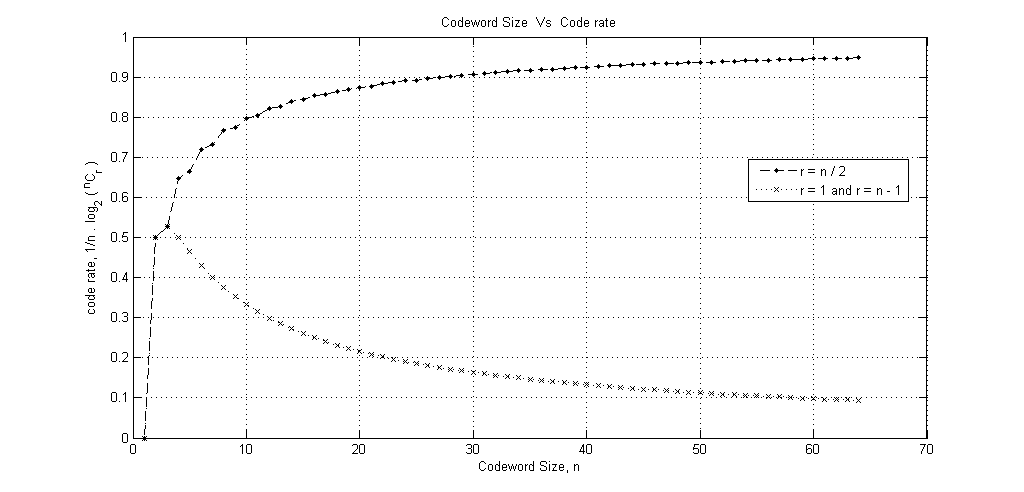
\includegraphics[width=\textwidth]{./Figures/max_min_coderate.png}
	\caption[Coderate limits imposed by $n$]{Upper and lower limits on coderate as function of frame size, n}
	\label{fig:coderate_limits}
\end{figure}

One more interesting result is the relationship between data transmission rate and the brightness index. The graph in figure \ref{fig:coderate_brightness} depicts the variations in coderate at different frame size $n$, where $n \in \{8, 16, 32, 64 \}$. The curve for fixed $n$ takes bell shape. Its the direct result of combinatorial relationship between frame size and brightness index, stated as $\binom{n}{r}=\binom{n}{n-r}$. The graph shows that the datarate is maximum in the middle of the curve where brightness index is $50\%$. The curves for different $n$ are farther apart from each other at this point which shows that the increased frame size has more pronounced increase in coderate when $r=\frac{n}{2}$ 


\begin{figure}[h]
	\centering
	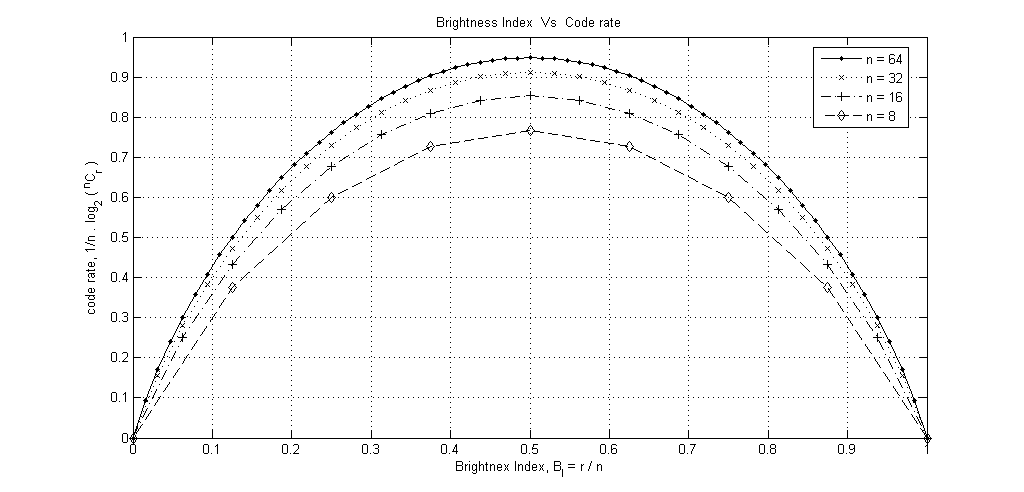
\includegraphics[width=\textwidth]{./Figures/coderate_brightness.png}
	\caption{Dependence of code-rate on brightness index}
	\label{fig:coderate_brightness}
\end{figure}


\section{Optimal Frame Size And Channel Conditions}
 It has been discussed earlier that both the brightness resolution and information carrying capacity of the VR-MPPM code improves when frame size is increased. However the symbol error probability also increases with the number of slots per frame, $n$. Therefore the frame size can not be increased arbitrarily. The effect can be observed by the relationship between single bit error probability, $p_e$ and the symbol decoding error probability, $p_s$ given be equation \ref{eq:error_probability}:

\begin{equation}
p_s=\left[1-(1-p_e)^n \right]
\label{eq:error_probability}
\end{equation}

The probability of correctly detection of a symbol given be the equation \ref{eq:correction_probability}, decreases with increasing frame size $n$. The parameter $p_{s,corr}$ is plotted for two different values of single bit error probability $p_e$ in figure \ref{fig:symbol_error}

\begin{equation}
 p_{s,corr}=\bar{p}_s=(1-p_e)
\label{eq:correction_probability}
\end{equation}

\begin{figure}[h]
	\centering
	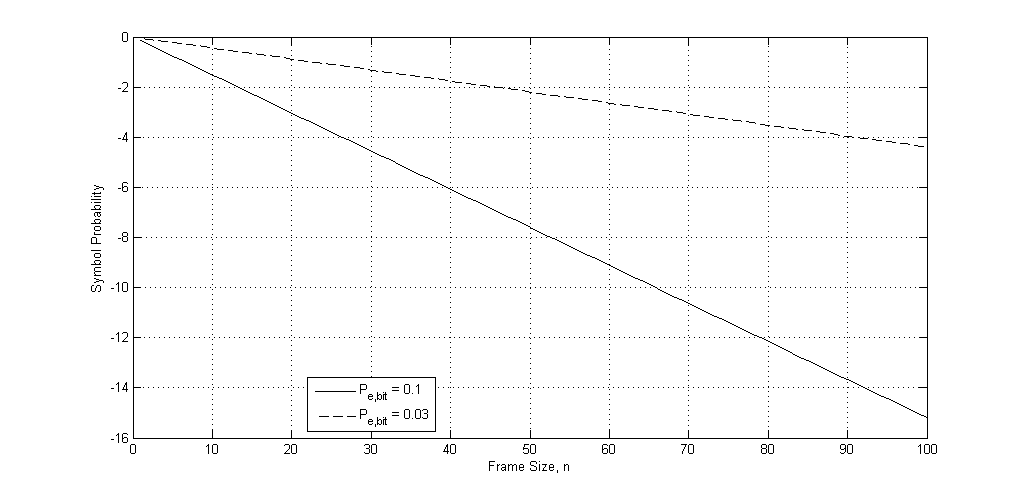
\includegraphics[width=\textwidth]{./Figures/SymbolVsn.png}
	\caption[Symbol correctly decoding probablity]{Symbol correctly detection probability as a function of frame size}
	\label{fig:symbol_error}
\end{figure}

It is aimed that the encoding scheme should provide maxim datarate and maximum control over brightness levels with minimum symbol error count.These contradictory requirements point towards finding an optimal size of the codeword such that the brightness resolution and symbol correctly detection probability $p_{s,corr}$ are maximum possible. It leads to the evaluation of the optimization problem defined by equation \ref{eq:objective_function}. The objective function is plotted for two bit error probabilities in figure \ref{fig:objective_function}. Peak values in the graph indicate the optimal frame size for a given value of bit error probability $p_e$

\begin{figure}
	\centering
	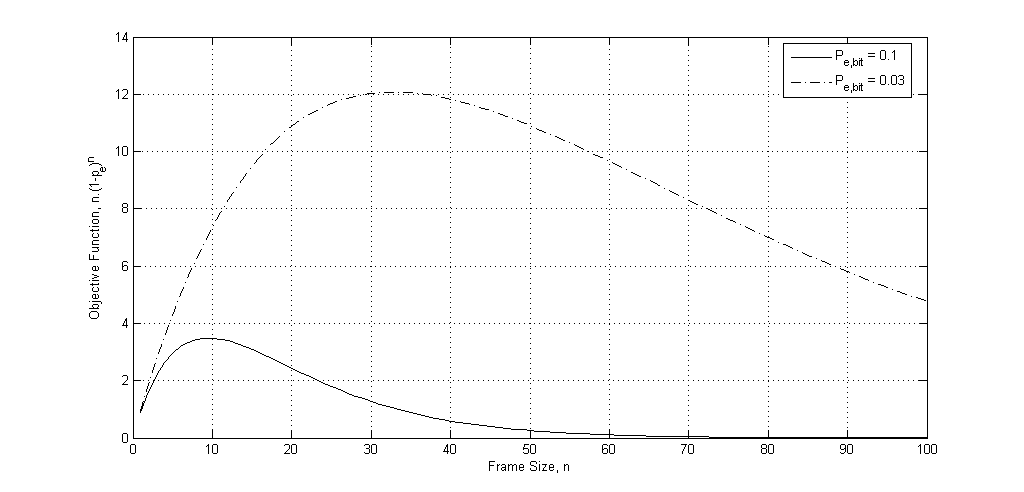
\includegraphics[width=\textwidth]{./Figures/ObjectiveFunction.png}
	\caption{Encoder frame size objective function}
	\label{fig:objective_function}
\end{figure}

\begin{equation}
\begin{array}{cc}
\mathbf{maximize}& f(n)=n(1-p_e)^n \\
\mathbf{subject~to}& 0<n, 0 \leq p_e \leq 1
\end{array}
\label{eq:objective_function}
\end{equation}

The value of $n$ in equation \ref{eq:objective_function} can be relaxed to be a positive integer as it defines the number of bits in a codeword. To check for global optimality of the solution given by objective function, its second derivative is evaluated as

\begin{equation}
f''=(\bar{p}_e)^n \ln (\bar{p}_{s,corr})(n \ln \bar{p_e} + 2)
\label{eq:second_d}
\end{equation}

Where $\bar{p}_e=(1-p_e)$ in equation \ref{eq:second_d}. The objective function based upon \ref{eq:second_d} is identified as

\begin{equation}
    f(n) = \left\{\begin{array}{cccc}
    concave & as~ f''(n) \leq 0  & for & \frac{2}{|\ln (1-p_e)|} \geq n \\
    convex & as~ f''(n) \geq 0  & for & \frac{2}{|\ln (1-p_e)|} \leq n
\end{array}   \right..
\label{eq:concavity}
\end{equation}

The solution for equation \ref{eq:objective_function} finally evaluates as

\begin{equation}
\psi (n) = \frac{1}{n}
\end{equation}

The optimality function $\psi(n)$ is plotted as a function of channel bit transitional probability $p_e$ in figure \ref{fig:optimal_function}


\begin{figure}{htbp}
	\centering
	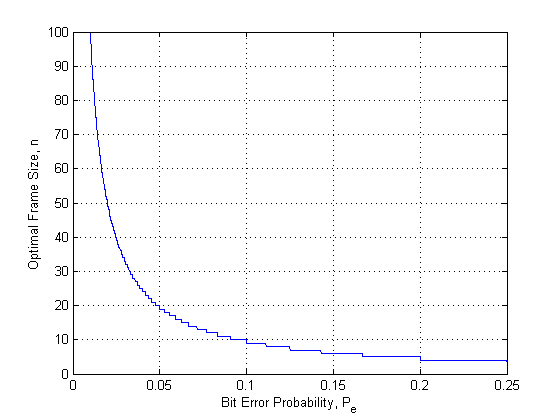
\includegraphics[width=\textwidth]{./Figures/OptimalFunction.png}
	\caption{Optimal value of frame size Vs Bit transition probability}
	\label{fig:optimal_function}
\end{figure}
%=======================================
The curve provides the optimal number of bits per codeword for a given channel bit transition probability $P_e$ on horizontal axis.

%\section{Hardware Implementation}
%Effectiveness of the proposed solution was shown by hardware implementation. We did hardware test on two platforms. The first implementation uses the RS232 protocol to drive the light source. The second implementation is the FPGA implementation using Digilent Nexys-2 FPGA board \cite{nexys2}.
%
%\section{RS-232 Based Implementation}
%First one implements the variable rate pulse position modulation (VR-MPPM) using byte transmission in UART communication. A USB to UART cable was used to interface the transmitter and receive modules to the computer. The converter cable used Texas Instruments chip TUSB3410\cite{TUSB3410} that supports speeds upto 921600 baud. The transmitter consists of 84 high brightness white LEDs mounted in grid form of $6\times 14$ LED. 14 LED are connected in parallel in a string. Three such strings are connected in series connection to form a $3\times 14$ LED bank. That means a bank of LEDs can be lighted from a 12V DC wall adapter. Two such banks are connected in parallel in the transmitter shown in figure \ref{fig:tx_hardware}. Texas Instruments' half-bridge bipolar switching integrated circuit UC2950T \cite{UC2950} is used as power driver.
%
%\begin{figure}[hbtp]
%\centering
%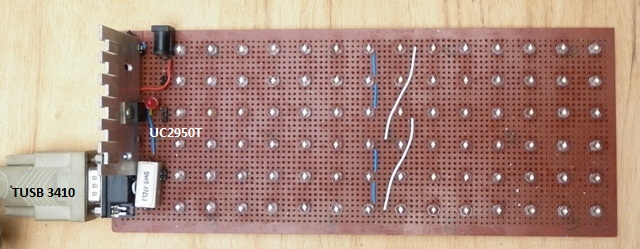
\includegraphics[angle=0,width=0.9\textwidth]{./Figures/Transmitter.jpg}
%\caption[VLC transmitter hardware]{VLC transmitter light consists of 84 High brightness White light LED}
% \label{fig:tx_hardware}
%\end{figure}
%
%The receiver module is built around toshiba TORX173 \cite{TORX173} optical fiber receiver for digital audio. This particular module is easily available in the market. It provides clean TTL electrical output signal  that is stabilized over wide range of optical signal power level. This makes the interfacing with TUSB3410 \cite{TUSB3410}, USB to UART converter, hassle free. The optical receiver module supports data rates upto 6MHz that covers full range of the converter and LED driver chips. Receiver module is shown in figure \ref{fig:rx_hardware}. 
%
%\begin{figure}[hbtp]
%\centering
%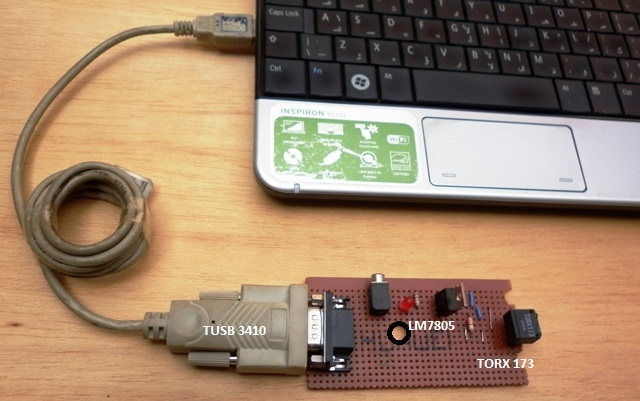
\includegraphics[angle=0,width=0.75\textwidth]{./Figures/Receiver_v2.jpg}
%\caption[VLC receiver hardware]{VLC receiver built around Toshiba TORX173 integrated optical receiver module}
%\label{fig:rx_hardware}
%\end{figure}
%
%%The hardware setup is used to evaluate the symbol error probability at different brightness indices. The graph in figure \ref{fig:evaluation1_hardware} shows the relationship. It is observed that minimum symbol error rate is achieved at around $0.5$ brightness index. Beyond that point on either side error probability is higher due to saturation of the receiver owing to unbalanced one-zero stream.
%%\begin{figure}
%%	\centering
%%	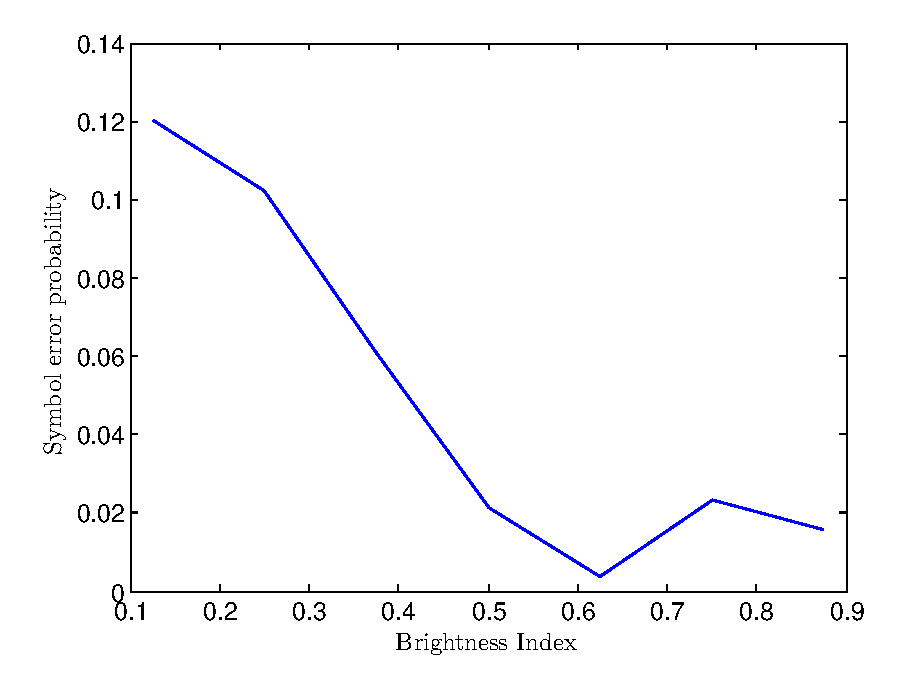
\includegraphics[width=\textwidth]{./Figures/experiment_brightness}
%%	\caption[Effect of brightness index on symbol error rate]{Practical evaluation: Effect of brightness index on symbol error rate}
%%	\label{fig:evaluation1_hardware}
%%\end{figure}
%
%
%\section{FPGA implementation on Xilinx Spartan-3 board}
%
%Although UART based implementation is easier to set up as this protocol has been one of the most popular data interfacing schemes and is already supported by a lot of devices however brightness control in this implementation is limited. The start and stop bits inserted by the protocol introduce extra time slots whose value can not changed according to the desired brightness level.
%
%To test the effectiveness of the proposed solution we implemented the VR-MPPM scheme using FPGAs. This implementation was used to evaluate the data rate and error performance of the proposed codes over more wider range of frame size and brightness indices. This implementation provides better control over brightness level along with faster data transmission as overhead bits do not effect the output stream. The prototype is set up in loop-back fashion with both the encoder and the decoder implemented on Nexys-2 \cite{nexys2} board from digilent. This board hosts Xilinx Spartan 3E-500 FG320 FPGA chip.  Verilog Hardware Description Language (HDL) was used to implement the logic. Hardware is described at behavioural level therefore no significant difference is there between the earlier listed algorithms \ref{algo:Encoder} \ref{algo:Decoder}  and the Verilog HDL code.
%
%%\begin{figure}[hbtp]
%%\centering
%%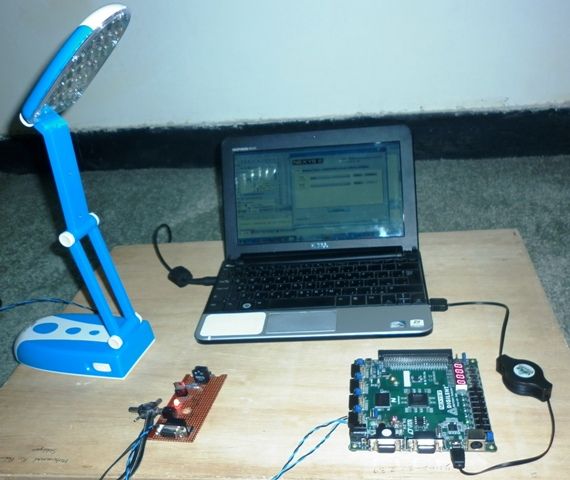
\includegraphics[angle=0,width=0.75\textwidth]{./Figures/Lamp_Off.jpg}
%%%\caption{VLC setup with Nexys-2 Development Board}
%%\label{fig:VLCNexys2On}
%%\end{figure}
%%
%%
%%\begin{figure}[hbtp]
%%\centering
%%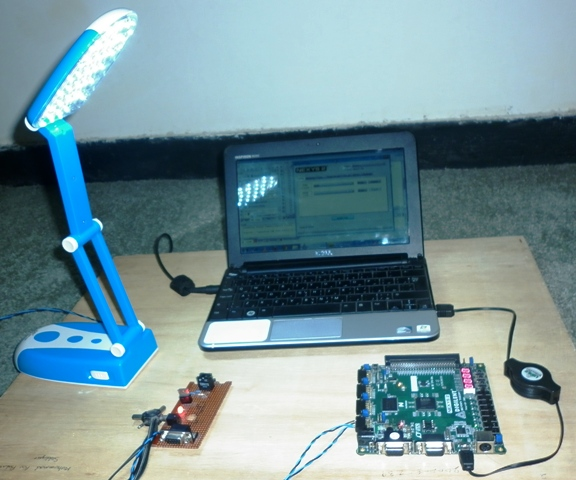
\includegraphics[angle=0,width=0.75\textwidth]{./Figures/Lamp_On.jpg}
%%\caption{VLC setup with Nexys-2 Development Board}
%%\label{fig:VLCNexys2Off}
%%\end{figure}
%
%
%
%\begin{figure}[hbtp]
%\centering
%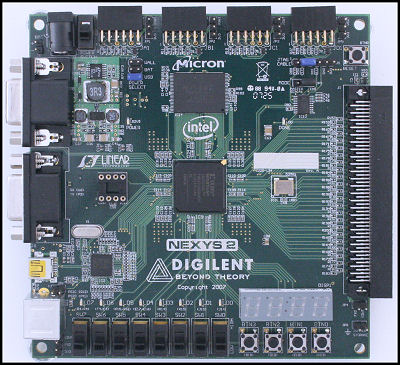
\includegraphics[angle=0,width=0.75\textwidth]{./Figures/NEXYS2_400.jpg}
%\caption{Nexys-2 Development Board}
%\label{fig:nexy2}
%\end{figure}
%
%\subsection{Encoder Module}
%The encoder implements the algorithm discussed in Chapter-\ref{Chapter3} algorithm:\ref{algo:Encoder}. It requires 'n' clock cycles to convert the input symbol to n-bit codeword sequentially. The combinatorial function required by the encoder $binom{n}{r}$ is implemented using the lookup table. Same lookup table is used by the decoder as well. This table is implemented in a separate module \textbf{nCrROM} as listed in appendix \ref{sec:nCrROM}. The encoder evaluates the most significant bit first and provides encoded data both in serial and parallel form. The $complete$ signal is asserted after encoding process is complete. Parallel output can be read correctly after this signal is set. Encoding process is started after detecting a high level on $start$ input at positive clock edge. Signal $m$ is the input signal that is coded with bits defined by $frameSize$. The output codewords is generated with $r$ pulses slots.
%\begin{figure}[h]
%	\centering
%%	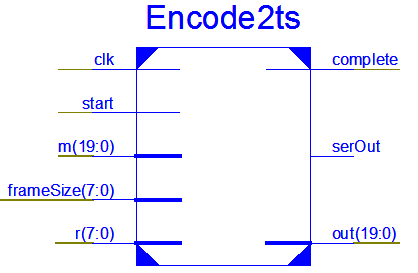
\includegraphics{./Figures/Encode2ts.png}
%	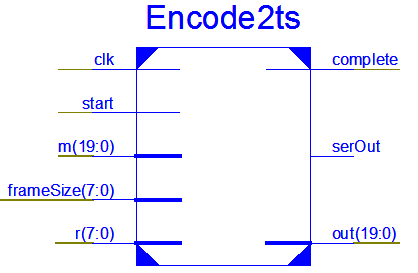
\includegraphics[width=.5\textwidth]{./Figures/Encode2ts.png}
%	\caption{VR-MPPM encoder module}
%	\label{fig:Encode2ts}
%\end{figure}
%\subsection{Decoder Module}
%The decoder is implemented using algorithm \ref{algo:Decoder}. Decoder, too, requires 'n' clock cycles to convert the n-bit input codeword back to the original symbol. It evaluates the most significant bit first. Therefore encoder and decoder module can work back to back with a serial link. The decoder can also take in the codeword as a parallel word. It is read in at positive clock edge after the signal $start$ is set. All other signals are same as described for the encoder.
%
%\begin{figure}[h]
%	\centering
%%	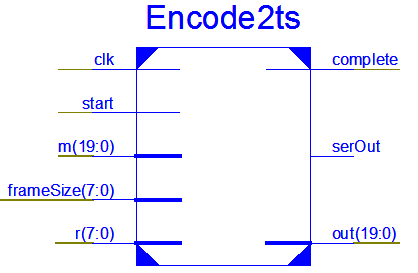
\includegraphics{./Figures/Encode2ts.png}
%	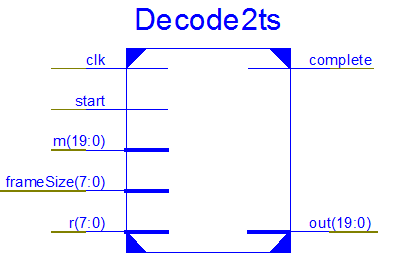
\includegraphics[width=.5\textwidth]{./Figures/Decode2ts.png}
%	\caption{VR-MPPM decoder module}
%	\label{fig:Decode2ts}
%\end{figure}
%
%\subsection{Parallel to Serial and Serial to Parallel Module}
%The functionality of this module is to transmit and receive the parallel data on an external serial link. Serial link in this case consisted of the visible light communication optical link. Because we needed to check the link performance for VR-MPPM at different frame sizes and brightness indices, serial data was sent on $serOut$ at positive clock edge and read in through $serIn$ on negative edge of the clock. The Nexys-2 boards's Pmod port JA1 was used to transmit and receives the data on serial link consisting of white light LED and TORX-173 optical receiver. The Verilog implementation is listed in appendix \ref{sec:p2p}
%\begin{figure}[h]
%	\centering
%	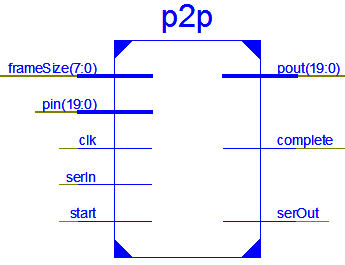
\includegraphics[width=.5\textwidth]{./Figures/p2p.png}
%	\caption{Serial link module}
%	\label{fig:p2p}
%\end{figure}
%
%\subsection{Encoded Parallel$\leftrightarrow$Serial Module}
%This is an upper level module that integrates the encoder, p2p and encoder module, thus completing the serial link with VR-MPPM encoded data. As encoder and decoder operate at very high nexys-2 board frequency, this module generates a slower clock frequency suitable for white LED operation. The input word $pin$ is first encoded using encoder module \ref{sec:Encode2ts}. When this conversion is complete it is sent over serial link using p2p module \ref{sec:p2p}. After parallel$\leftrightarrow$Serial complete signal is asserted the data is received in completely and is fed to the decoder module \ref{sec:Decode2ts}. This module's $complete$ signal is asserted after all the three stages have been completed.
%
%\begin{figure}[h]
%	\centering
%	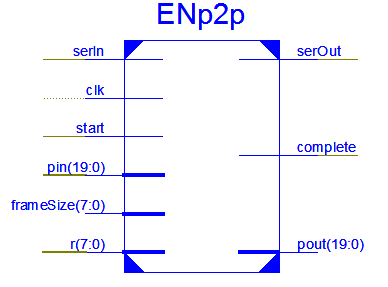
\includegraphics[width=.5\textwidth]{./Figures/ENp2p.png}
%	\caption{VR-MPPM encoded serial link module}
%	\label{fig:ENp2p}
%\end{figure}
%
%\subsection{Module for Scanning VLC Codes}
%The scan codes \ref{sec:scanCodes} module was implemented to check the error rate performance of the optical link by cycling through all possible symbols in cyclic form, for a particular selection of frame size and brightness index. This module keeps record of the error count by comparing the received and transmitted symbols.
%
%\begin{figure}
%	\centering
%	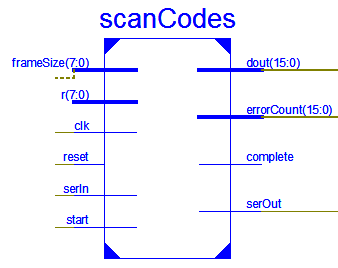
\includegraphics[width=.5\textwidth]{./Figures/scanCodes.png}
%	\caption[Module for generating scan symbols]{Generate VR-MPPM symbols for onboard evaluation of bit error rate}
%%	\caption{HDL block to generate, transmit and receive VR-MPPM symbols for onboard evaluation of bit error rate}
%	\label{fig:scanCodes}
%\end{figure}
%
%\subsection{VLC Module}
%VLC is the top level module. It defines the ports and signals of the Nexys-2 board that are used during actual functionality test. The user constraint file $toplevel.ucf$ \ref{sec:toplevel} defines the mapping of board ports to VLC module signals.
%
%
%%\begin{figure}[hbtp]
%%\centering
%%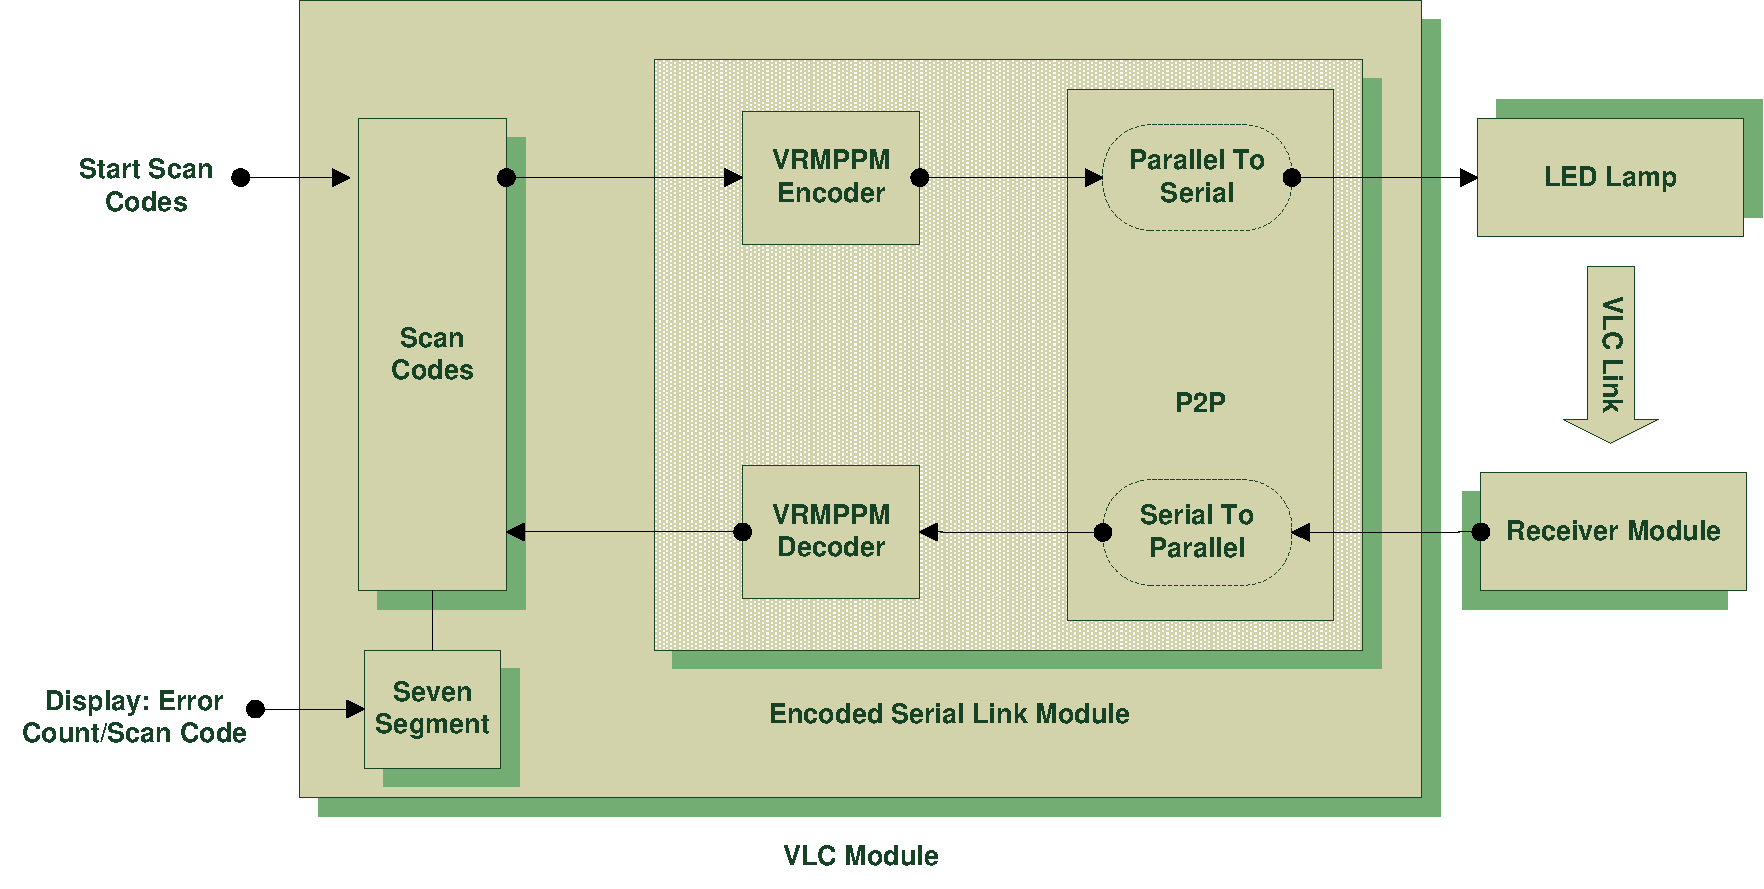
\includegraphics[angle=0,width=\textwidth]{./Figures/VLC_block_diagram}
%%\caption{FPGA Implementation Block Diagram}
%%\label{fig:FPGAblock}
%%\end{figure}
%
%%\subsection{User Constraints File}
%%The constriant file \ref{sec:toplevel} for Nexys-2 board defines the pins used for VLC module signals.
%
%\begin{figure}[h]
%	\centering
%	\includegraphics[width=.5\textwidth]{./Figures/vlc.png}
%	\caption[Toplevel VLC module]{HDL block diagram of top level module for serial link simulation}
%	\label{fig:vlc}
%\end{figure}
%
%\subsection{Clock Divider Module}
%The basic clock of Nexys-2 board runs at 50MHz. This frequency is much higher than the capability of commonly available white LEDs. Therefore it is requiered to slow down the actual transmitting frequency to within a few megahertz. The clock divider module \textbf{clkDiv} takes in the system clock signal and outputs a new clock that is slowed down by the count value defined by the input word $newDiv$.
%
%\begin{figure}[h]
%	\centering
%	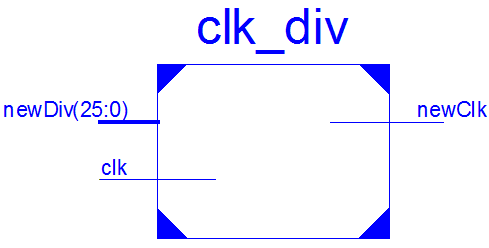
\includegraphics[width=.5\textwidth]{./Figures/clk_div.png}
%	\caption[]{Clock divider module}
%	\label{fig:clkDiv}
%\end{figure}
%
%
%\subsection{Seven Segment Driver Module} The Nexys-2 board houses a four digit seven segment display. This module drives the display to represent 16-bit word in hexadecimal format \ref{sec:LED_7seg}.
%
%\begin{figure}[h]
%	\centering
%	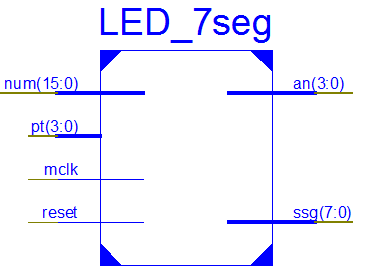
\includegraphics[width=.5\textwidth]{./Figures/LED_7seg.png}
%	\caption{7-segment drivier module to display 16-bit values }
%	\label{fig:LED_7seg}
%\end{figure}
%
%\section{Experimental Results}
%
%The performance of a VR-MPPM visible light link at different brightness indices was evaluated using a FPGA platform. Transmitter and Receiver module were implemented on Digilent's Nexys-2 board. The transmitter consisted of off the shelf white LEDs. The receiver was built around TORX173 optical receiver module from Toshiba. Receiver and transmitter were interfaced to the Nexys-2 board using two interface lines of the $JA$ pmod connector. Symbol error rate was observed for three different values of frame size by varying the brightness index in the available range. The results are represented in figure \ref{fig:fpgaExperiment}. It can be observed that code error performance degrades for larger frame size at fixed brightness index, as depicted by equation \ref{eq:error_probability}.
%
%\begin{figure}[h]
%	\centering
%	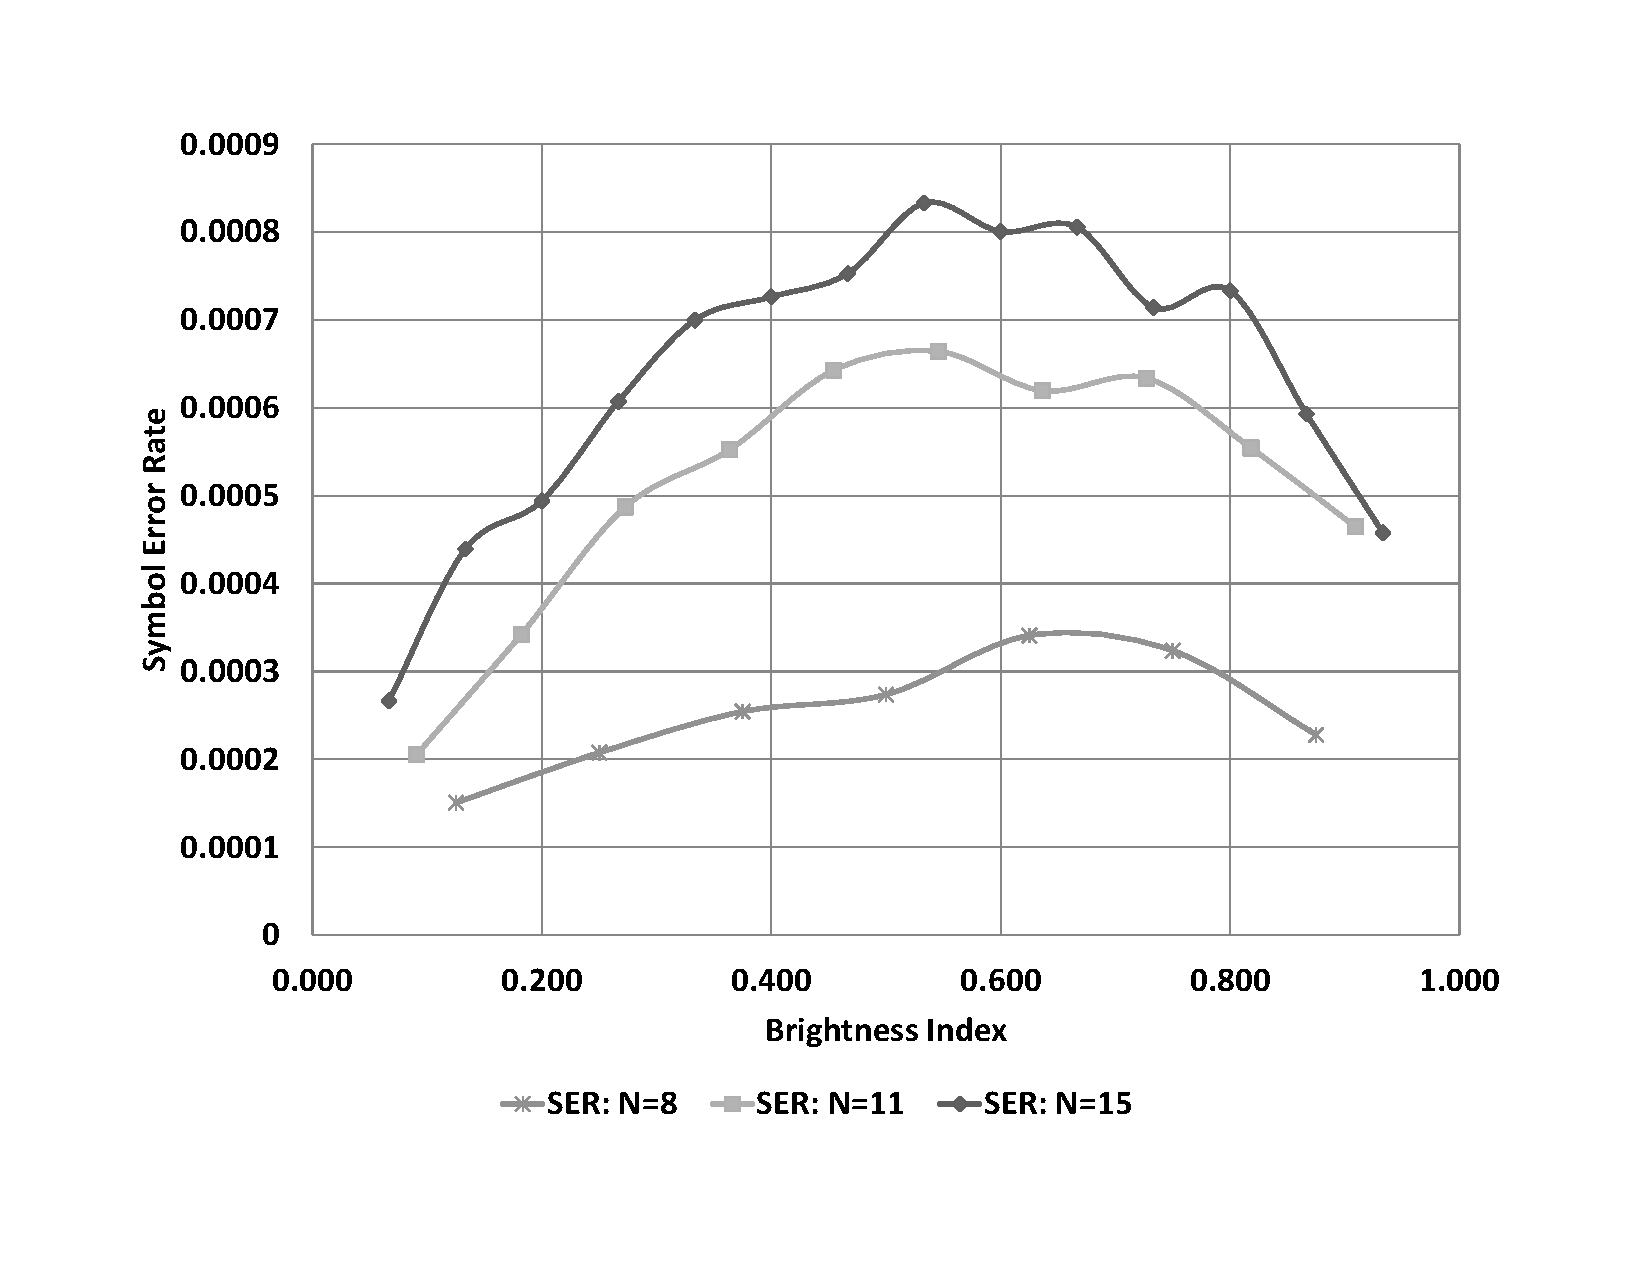
\includegraphics[width=\textwidth]{./Figures/Experiment}
%	\caption[Hardware Performance Evaluation]{Symbol error rate evaluation of VR-MPPM encoded symbols at different brigness indices. $n$ represents the frame size.}
%	\label{fig:fpgaExperiment}
%\end{figure}
%
%For a given frame size, the symbol error rate curve takes a bell shaped curve with maximum number of errors encountered around 50\% brightness. From discussion of the proposed VR-MPPM codes it is known that maximum bit transitions occur for 50\% brightness as shown in figure \ref{Fig:line_codes2}. There are more bandwidth constraints on a fast switching signal. That counts for the greater number of errors.
%
%The experimental results are also in close agreement to the MPPM channel modelling presented in \cite{hamkins2005multipulse}. 
%
%%
%%Let $p_0(y)$ denotes the conditional probability of decoding a bit as 'y' when a zero was transmitted and $p_1(y)$ is the probability of decoding 'y' when a one was transmitted. Suppose in a frame size consisting of 'n' time slots of which first 'r' time slots contain a one and last 'n-r' slots contain a zero. Considering the discrete memory less channel with hard detection, the probability of decoding error of a symbol 's' is given by:
%%
%%\[
%% P_{ser} = (probability~of~1\rightarrow 0~transition)^r \times  (probability~of~0\rightarrow 1~transition)^{n-r} 
%%\]
%%
%%Now there are a total of $2^n$ codewords possible with $n$ slots. We need to calculate the probability for $\binom{n}{r}$ symbols in group of total possible symbols. It provides with the probability of symbol decoding error with $r$ ones as
%%
%%\[
%% P_{ser,r} = \frac{1}{2^n} \binom{n}{r}(probability~of~1\rightarrow 0~transition)^r \times  (probability~of~0\rightarrow 1~transition)^{n-r} 
%%\]
%%
%%
%%\begin{equation}
%% P_{ser,r} = \frac{1}{2^n} \binom{n}{r} p_1^r(0) \times  p_0^{n-r}(1) 
%%\label{eq:ser2}
%%\end{equation}
%%
%%Equation \ref{eq:ser2} hints at a bell shaped curve for symbol error rate performance.
%
%
%
%\begin{figure}[h]
%\centering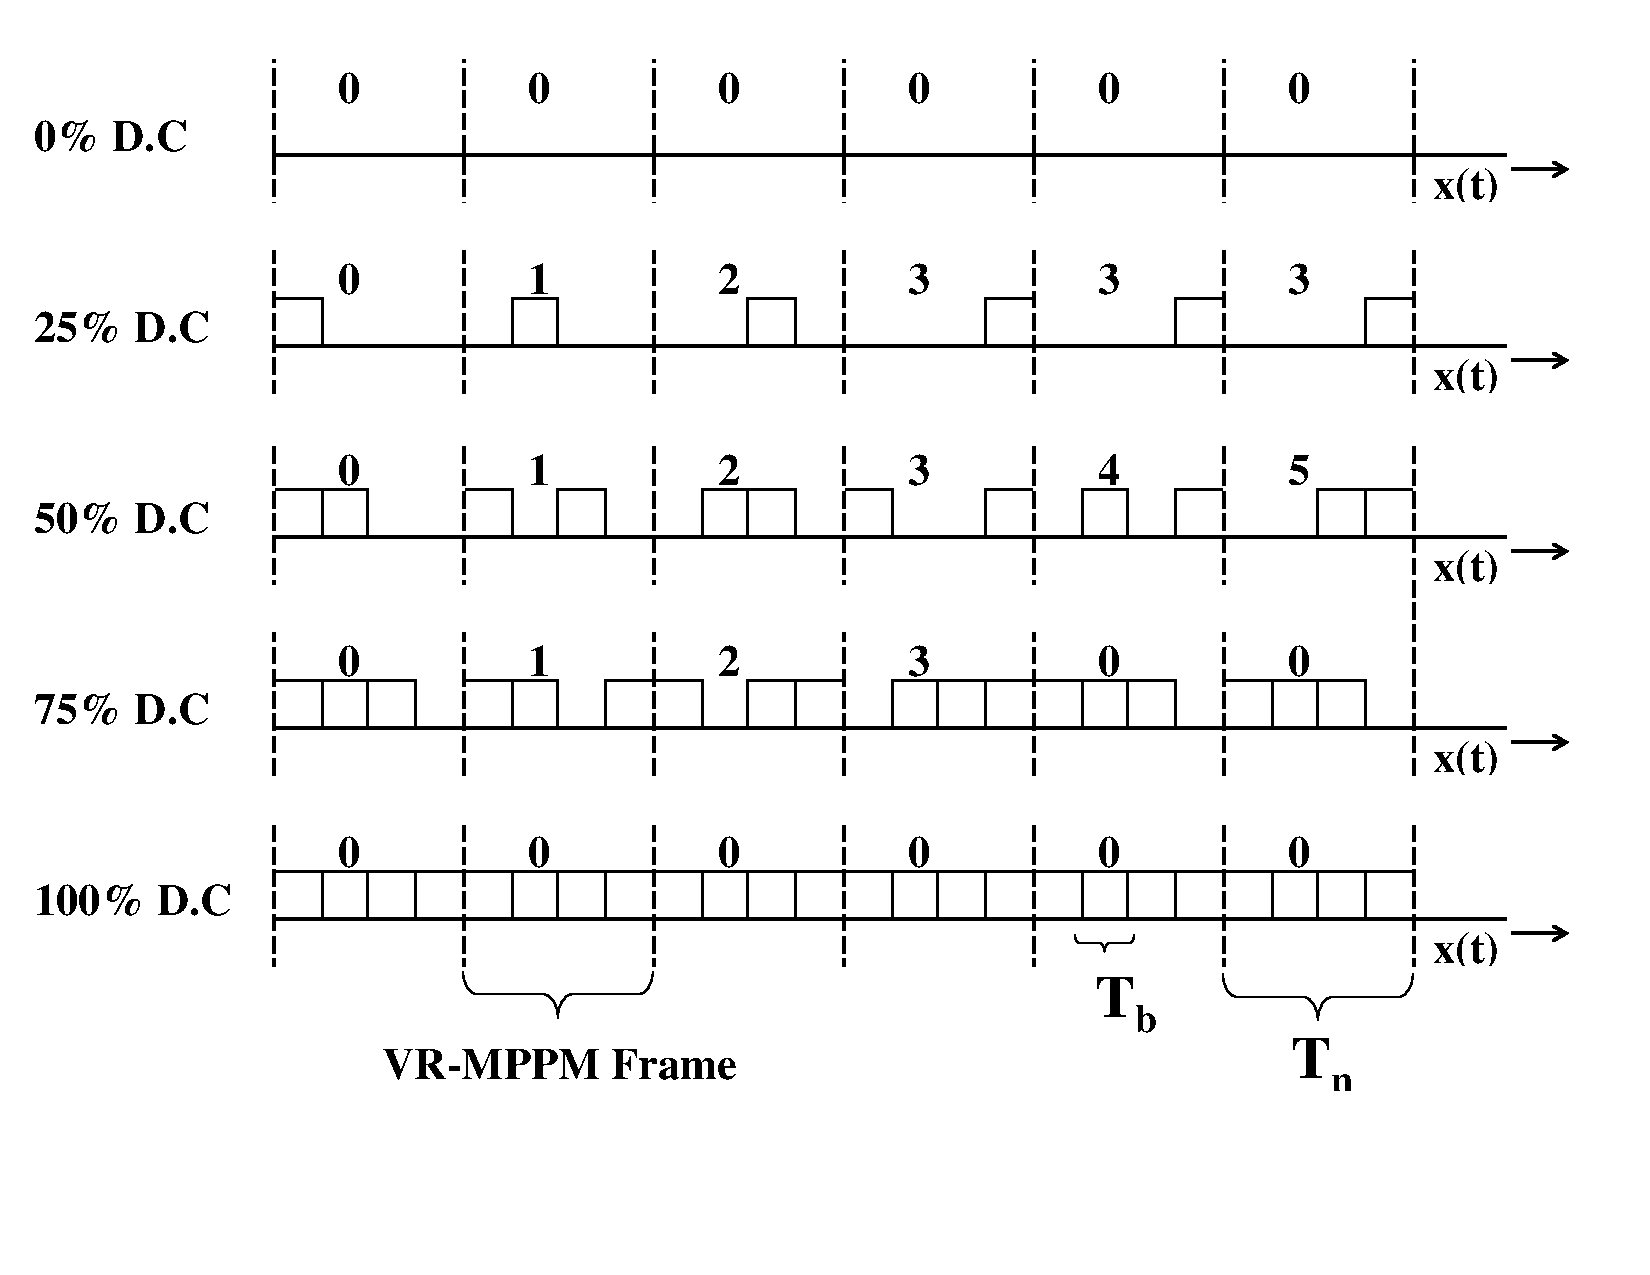
\includegraphics[width=\textwidth]{./Figures/line_code}
%\caption[VR-MPPM line waveforms]{VR-MPPM waveforms: Maximum transitions occur at 50\% brightness}
%\label{Fig:line_codes2}
%\end{figure} % Experiment 2

%% Chapter 5
% add following line for typesetting from subfiles
% !TeX root = ../uet_thesis.tex
% !TeX root = ../uet_thesis.bbl
% !TeX root = ../references.bib
\chapter{Implementation and Performance Evaluation} % Write in your own chapter title
\label{Chapter6}
\lhead{Chapter 6. \emph{Implementation and Performance Evaluation}} % Write in your own chapter title to set the page header
%\section{Introduction}


%5)	Implementation and performance evaluation (Harsware + Error Probability)
%i)	Transmitter
%ii)	Receiver
%iii)	Practical results: P_e Vs Brightness Index
%iv)	Maximization Problem

%%%\section{Data Transmission Rate}
%%%The information carrying capacity of the proposed codes is affected by the selection of the codeword. A larger code size ensures more brightness levels and better information carrying capacity per symbol frame. In this section we would see the effect of codeword size and brightness index on information carrying capacity of the VR-MPPM codes.
%%%
%%%The code rate varies when brightness index is changed. Code rate is minimum for $r=1$ and $r=n-1$. The former case is the simple pulse position modulation encoding that provides effective code rate of $\lfloor \frac{1}{n} \log_2 \binom{n}{1} \rfloor$ while the later is the inverted pulse position modulation. Its code rate is same as that of PPM however it drives the light source at illumination level near peak value. Maximum data rate is achieved when brightness index is $0.50$ that is $r=\frac{n}{2}$ giving effective code rate value of $\lfloor \frac{1}{n} \log_2 \binom{n}{n/2} \rfloor$.  The relationship of the two parameters with frame size, plotted in figure \ref{fig:coderate_limits}, provides important insight for system design. It can be observed that the code efficiency decreases at lower brightness indices when frame size is increased. However the maximum code rate improves with larger frame size. It tends to approach unity as frame size is increased.
%%%
%%%The code-rate for brightness index = 0.5 can be applied in other line coding applications as well. In those cases the VR-MPPM code ensures $50\%$ duty cycle over one symbol frame that provides DC null and code transparency. The maximum number of consecutive ones or zero's comes out to be $2(n-1)$ in this case. The code rate will be about doubled as compared to Manchester or phase encoding.
%%%
%%%\begin{figure}[!htbp]
%%%	\centering
%%%	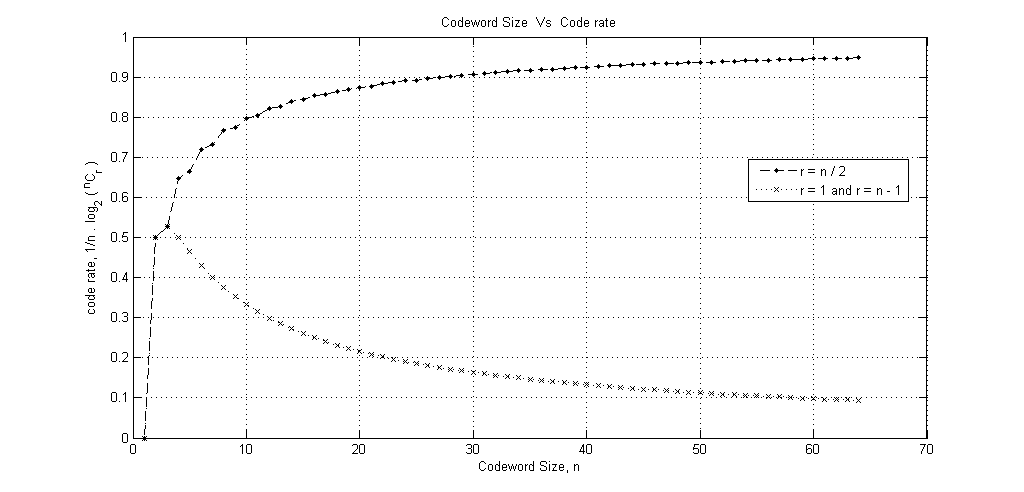
\includegraphics[width=\textwidth]{./Figures/max_min_coderate.png}
%%%	\caption[Coderate limits imposed by $n$]{Upper and lower limits on coderate as function of frame size, n}
%%%	\label{fig:coderate_limits}
%%%\end{figure}
%%%
%%%One more interesting result is the relation ship between data transmission rate versus the brightness index. The graph in figure \ref{fig:coderate_brightness} plots the code rate curves for different values of frame size. A curve for fixed $n$ is bell shape that results from the combinatorial mathematics relationship which states  $\binom{n}{r}=\binom{n}{n-r}$. It shows that the selection of larger frame size does not improve code rate by large degrees for brightness indices near the extreme values.
%%%
%%%\begin{figure}[!htbp]
%%%	\centering
%%%	\includegraphics[width=\textwidth]{./Figures/coderate_brightness.png}
%%%	\caption{Dependence of code-rate on brightness index}
%%%	\label{fig:coderate_brightness}
%%%\end{figure}
%%%
%%%
%%%\section{Optimal Frame Size And Channel Conditions}
%%% It has been discussed earlier that both the brightness resolution and information carrying capacity of the VR-MPPM code improve when frame size is increased. However the symbol error probability increases, too, with the number of bits per frame, $n$. Therefore the frame size can not be increased arbitrarily. The effect can be observed by the relation between the single bit error probability, $p_e$ and the symbol decoding error probability, $p_s$ given be equation \ref{eq:error_probability}:
%%%
%%%\begin{equation}
%%%p_s=\left[1-(1-p_e)^n \right]
%%%\label{eq:error_probability}
%%%\end{equation}
%%%
%%%The probability of correctly detection of a symbol, given be the equation \ref{eq:correction_probability}, decreases with frame size n. The parameter $p_{s,corr}$ is plotted for two different values of single bit error probability $p_e$ in figure \ref{fig:symbol_error}
%%%
%%%\begin{equation}
%%% p_{s,corr}=\bar{p}_s=(1-p_e)
%%%\label{eq:correction_probability}
%%%\end{equation}
%%%
%%%\begin{figure}
%%%	\centering
%%%	\includegraphics[width=\textwidth]{./Figures/SymbolVsn.png}
%%%	\caption[Symbol correctly decoding probablity]{Symbol correctly detection probability as a function of frame size}
%%%	\label{fig:symbol_error}
%%%\end{figure}
%%%
%%%These contradictory requirements point towards finding an optimal size of the codeword such that the brightness resolution and symbol correctly detection probability $p_{s,corr}$ are maximum possible. It leads to the evaluation of the optimization problem defined by equation \ref{eq:objective_function}. The objective function is plotted for two bit error probabilities in figure \ref{fig:objective_function}. Peak values in the graph indicate the optimal frame size for a given value of $p_e$
%%%\begin{figure}
%%%	\centering
%%%	\includegraphics[width=\textwidth]{./Figures/ObjectiveFunction.png}
%%%	\caption{Encoder frame size objective function}
%%%	\label{fig:objective_function}
%%%\end{figure}
%%%
%%%\begin{equation}
%%%\begin{array}{cc}
%%%\mathbf{maximize}& f(n)=n(1-p_e)^n \\
%%%\mathbf{subject~to}& 0<n, 0 \leq p_e \leq 1
%%%\end{array}
%%%\label{eq:objective_function}
%%%\end{equation}
%%%
%%%The value of $n$ in equation \ref{eq:objective_function} can be relaxed to be a positive integer as it defines the number of bits in a codeword. The check for global optimality of the solution given by objective function, we take its second derivative given as
%%%
%%%\begin{equation}
%%%f''=(\bar{p}_e)^n \ln (\bar{p}_{s,corr})(n \ln \bar{p_e} + 2)
%%%\label{eq:second_d}
%%%\end{equation}
%%%
%%%Where $\bar{p}_e=(1-p_e)$ in equation \ref{eq:second_d}. The objective function based upon \ref{eq:second_d} comes out to be
%%%
%%%\begin{equation}
%%%    f(n) = \left\{\begin{array}{cccc}
%%%    concave & as~ f''(n) \leq 0  & for & \frac{2}{|\ln (1-p_e)|} \geq n \\
%%%    convex & as~ f''(n) \geq 0  & for & \frac{2}{|\ln (1-p_e)|} \leq n
%%%\end{array}   \right..
%%%\label{eq:concavity}
%%%\end{equation}
%%%
%%%The solution for equation \ref{eq:objective_function} evaluates to be
%%%
%%%\begin{equation}
%%%\psi (n) = \frac{1}{n}
%%%\end{equation}
%%%
%%%The optimality function $\psi(n)$ is plotted as a function of channel bit transitional probability $p_e$ in figure \ref{fig:optimal_function}
%%%
%%%
%%%\begin{figure}
%%%	\centering
%%%	\includegraphics[width=\textwidth]{./Figures/OptimalFunction.png}
%%%	\caption{Optimal value of frame size Vs Bit transition probability}
%%%	\label{fig:optimal_function}
%%%\end{figure}

\section{Hardware Implementation}
Effectiveness of the proposed VR-MPPM line code is demonstrated by hardware implementation. A light source consisting of white LED grid is used as data transmitter paired with a receiver based upon an integrated photosensor module. The visible light wireless link is tested on two different platforms. The first implementation uses UART protocol to drive the light source. Serial port of a personal computer directly drives the LED circuit. The data bits in a UART packet are treated as one frame of VR-MPPM. Similarly at receiver end the photosensor module also directly connects to the PC serial port. The second implementation uses an FPGA board, Digilent Nexys-2\cite{nexys2}, and provides more freedom in selection of clock speed and frame size. Error performance of the visible light wireless link is evaluated by cycling through all possible codewords.

\section{UART Based Implementation}
The visible light wireless transmission implements VR-MPPM line code using byte frame of UART communication protocol. A USB to UART cable is used to interface the transmitter and receive modules to the computer. The converter cable is based upon Texas Instruments chip TUSB3410\cite{TUSB3410} that supports data speeds upto 921600 baud. The transmitter consists of 84 high brightness white LEDs mounted in grid form of $6\times 14$ LED. 14 LED are connected in parallel in a string. Three such strings are connected in series connection to form a $3\times 14$ LED bank. That means a bank of LEDs can be lighted from a 12V DC wall adapter. Two such banks are connected in parallel in the transmitter shown in figure \ref{fig:tx_hardware}. Texas Instruments' half-bridge bipolar switching integrated circuit UC2950T \cite{UC2950} is used as power driver.

\begin{figure}[hbtp]
\centering
\includegraphics[angle=0,width=0.9\textwidth]{./Figures/Transmitter.jpg}
\caption[VLC transmitter hardware]{VLC transmitter light consists of 84 High brightness White light LED}
 \label{fig:tx_hardware}
\end{figure}

The receiver module is built around toshiba TORX173 \cite{TORX173} optical fiber receiver for digital audio. This particular module is radily available in the local market. It provides clean TTL electrical output signal  that is stabilized over wide range of optical signal power levels. This makes the interfacing with TUSB3410 \cite{TUSB3410}, USB to UART converter, hassle free. The optical receiver module supports data rates upto 6MHz that covers full range of the converter and LED driver chips. Receiver module is shown in figure \ref{fig:rx_hardware}. 

\begin{figure}[hbtp]
\centering
\includegraphics[angle=0,width=0.75\textwidth]{./Figures/Receiver_v2.jpg}
\caption[VLC receiver hardware]{VLC receiver built around Toshiba TORX173 integrated optical receiver module}
\label{fig:rx_hardware}
\end{figure}

UART based implementation is easier to setup as this protocol has been a classic data interfacing scheme and is already supported by a large number of devices. However brightness resolution is limited in this implementation. There are always two extra start and stop bits in a UART frame, inserted for synchronization. Therefore the dimming range is limited from $10\%$  to $90\%$ of the full brightness level.


%The hardware setup is used to evaluate the symbol error probability at different brightness indices. The graph in figure \ref{fig:evaluation1_hardware} shows the relationship. It is observed that minimum symbol error rate is achieved at around $0.5$ brightness index. Beyond that point on either side error probability is higher due to saturation of the receiver owing to unbalanced one-zero stream.
%\begin{figure}
%	\centering
%	\includegraphics[width=\textwidth]{./Figures/experiment_brightness}
%	\caption[Effect of brightness index on symbol error rate]{Practical evaluation: Effect of brightness index on symbol error rate}
%	\label{fig:evaluation1_hardware}
%\end{figure}


\section{FPGA implementation on Xilinx Spartan-3 board}

The second performance test of the proposed VR-MPPM was evaluated on FPGA boards. This implementation was used to evaluate the data rate and error performance of the proposed codes over wider range of frame size and brightness indices. This implementation provided better control over brightness level along with faster data transmission as compared to the UART implementation. The prototype was setup in loop-back fashion with both the encoder and the decoder implemented on same Nexys-2 \cite{nexys2} FPGA board. This board hosts Xilinx Spartan 3E-500 FG320 FPGA chip.  Verilog Hardware Description Language (HDL) was used to implement the logic for VR-MPPM encoder, decoder and performance evaluation logic. Hardware is described at behavioural level therefore there is no significant difference between the earlier listed algorithms \ref{algo:Encoder} \ref{algo:Decoder} in Chapter-3 and the Verilog HDL code.

The LED light is operated at 500kHz clock. The brightness resolution (frame size) and brightness index are selectable from FPGA board. The test is performed by transmitting $10^6$ frames, cycling through all valid codes for the selected frame size and brightness index, and erroneous symbols are counted on the receiver. Symbol error probability is calculated as ratio of symbol error count and total transmitted symbols.
%\begin{figure}[hbtp]
%\centering
%\includegraphics[angle=0,width=0.75\textwidth]{./Figures/Lamp_Off.jpg}
%%\caption{VLC setup with Nexys-2 Development Board}
%\label{fig:VLCNexys2On}
%\end{figure}
%
%
%\begin{figure}[hbtp]
%\centering
%\includegraphics[angle=0,width=0.75\textwidth]{./Figures/Lamp_On.jpg}
%\caption{VLC setup with Nexys-2 Development Board}
%\label{fig:VLCNexys2Off}
%\end{figure}



\begin{figure}[hbtp]
\centering
\includegraphics[angle=0,width=0.75\textwidth]{./Figures/NEXYS2_400.jpg}
\caption{Nexys-2 Development Board}
\label{fig:nexy2}
\end{figure}

\subsection{Encoder Module}
The encoder module implements the hardware description of algorithm \ref{algo:Encoder} presented in Chapter \ref{Chapter3}. It requires 'n' clock cycles to convert the input symbol $m$ to n-bit codeword, with $n$ defined by the signal $frameSize$. The combinatorial function $\binom{n}{r}$ is required by the encoder that is implemented using lookup table technique. This table is accessed using a separate \textbf{nCrROM} module that is listed in appendix \ref{sec:nCrROM}. The encoder evaluates most significant bit first and provides encoded data both in serial and parallel formats. Encoding process is started by a high level on $start$ input at positive clock edge. The $complete$ signal is asserted after encoding process is finished. The calculated codewords contains $r$ 1's in the output signal $out$.
\begin{figure}[!htbp]
	\centering
%	\includegraphics{./Figures/Encode2ts.png}
	\includegraphics[width=.5\textwidth]{./Figures/Encode2ts.png}
	\caption{VR-MPPM encoder module}
	\label{fig:Encode2ts}
\end{figure}
\subsection{Decoder Module}
Decoder is implemented using algorithm \ref{algo:Decoder} in \ref{Chapter3}. This module also requires 'n' clock cycles to convert the n-bit input codeword back to the original symbol, evaluating the most significant bit first. Therefore encoder and decoder module can be made to work in back to back fashion with a serial link. In present implementation decoder takes in the codeword as a parallel input $m$. It is read at positive clock edge after the $start$ signal is set. Rest of the signals have same functionality as defined in encoder module.

\begin{figure}[!htbp]
	\centering
%	\includegraphics{./Figures/Encode2ts.png}
	\includegraphics[width=.5\textwidth]{./Figures/Decode2ts.png}
	\caption{VR-MPPM decoder module}
	\label{fig:Decode2ts}
\end{figure}

\subsection{Parallel to Serial and Serial to Parallel (p2p) Module}
It is an intermediate module between encoder and decoder modules. Its role is to transmit and receive parallel data on an external serial link. The serial link consists of the visible light communication signal. To check the link performance of VR-MPPM at different frame sizes and brightness indices, serial data is sent out $serOut$ signal at positive clock edge that is read in through $serIn$ signal on negative edge of the clock. The signal $frameSize$ determines the frame size of serial output. The Nexys-2 boards' Pmod port $JA1$ is used to transmit and receives the data on serial link consisting of white LEDs and TORX-173 optical receiver. Verilog implementation of the module is listed in appendix \ref{sec:p2p}. The $clk$ input signal determines the bit time of the optical serial signal. This signal is helpful for evaluating code performance at different frequencies.
\begin{figure}[!htbp]
	\centering
	\includegraphics[width=.5\textwidth]{./Figures/p2p.png}
	\caption{Serial link module}
	\label{fig:p2p}
\end{figure}

%\subsection{Encoded Parallel$\leftrightarrow$Serial (ENp2p) Module}
\subsection{Encoded Parallel-Serial (ENp2p) Module}
This is an upper level module that integrates the encoder, p2p and encoder modules, thus completing the serial link with VR-MPPM encoded data. As encoder and decoder operate at primary clock frequency of the FPGA board, this module sets clock frequency suitable for white LED operation. The internal signal flow in this module takes place according to following sequence: Input word $pin$ is first encoded using encoder module \ref{sec:Encode2ts}. When this conversion is complete encoded word is sent over serial link using p2p module \ref{sec:p2p}. After parallel$\leftrightarrow$Serial$\leftrightarrow$Parallel through optical link operation is complete and serial data has been received completely, it is fed to the decoder module \ref{sec:Decode2ts}. Decoder module's $complete$ signal is asserted after all the three stages are completed.

\begin{figure}[!htbp]
	\centering
	\includegraphics[width=.5\textwidth]{./Figures/ENp2p.png}
	\caption{VR-MPPM encoded serial link module}
	\label{fig:ENp2p}
\end{figure}

\subsection{Module for Scanning VLC Codes}
The scan codes \ref{sec:scanCodes} module is implemented to check the error rate performance of the optical link by cycling through all possible symbols for a particular selected frame size and brightness index. This module works on top of \textbf{ENp2p} module and keeps record of the errors encountered by comparing the received and transmitted symbols.

\begin{figure}
	\centering
	\includegraphics[width=.5\textwidth]{./Figures/scanCodes.png}
	\caption[Module for generating scan symbols]{Generate VR-MPPM symbols for onboard evaluation of bit error rate}
%	\caption{HDL block to generate, transmit and receive VR-MPPM symbols for onboard evaluation of bit error rate}
	\label{fig:scanCodes}
\end{figure}

\subsection{VLC Module}
VLC is the top level module. It defines the ports and signals of the Nexys-2 board that are used for external hardware intrfacing during actual functionality test. The user constraint file $toplevel.ucf$ \ref{sec:toplevel} defines the mapping of board ports to input\/output  signals.


%\begin{figure}[hbtp]
%\centering
%\includegraphics[angle=0,width=\textwidth]{./Figures/VLC_block_diagram}
%\caption{FPGA Implementation Block Diagram}
%\label{fig:FPGAblock}
%\end{figure}

%\subsection{User Constraints File}
%The constriant file \ref{sec:toplevel} for Nexys-2 board defines the pins used for VLC module signals.

\begin{figure}[!htbp]
	\centering
	\includegraphics[width=.5\textwidth]{./Figures/vlc.png}
	\caption[Toplevel VLC module]{HDL block diagram of top level module for serial link simulation}
	\label{fig:vlc}
\end{figure}

\subsection{Clock Divider Module}
The basic Nexys-2 board clock runs at 50MHz. This is too high frequency and is much higher than the capability of common available white LEDs. Therefore it is desired to divide down the origional clock to a transmitting frequency within few mega hertz. The clock divider module \textbf{clkDiv} takes in the system clock signal and outputs a new clock slowed down by the count value defined by the input word $newDiv$.

\begin{figure}[!htbp]
	\centering
	\includegraphics[width=.5\textwidth]{./Figures/clk_div.png}
	\caption[]{Clock divider module}
	\label{fig:clkDiv}
\end{figure}


\subsection{Seven Segment Driver Module} The Nexys-2 board houses a four digit seven segment display. This module drives the display to represent 16-bit word in hexadecimal format \ref{sec:LED_7seg}.

\begin{figure}[!htbp]
	\centering
	\includegraphics[width=.5\textwidth]{./Figures/LED_7seg.png}
	\caption{7-segment drivier module to display 16-bit values }
	\label{fig:LED_7seg}
\end{figure}

\section{Experimental Results}

The performance of a VR-MPPM visible light link at different brightness indices was evaluated using the FPGA platform. Transmitter and Receiver module were implemented on Digilent's Nexys-2 board. The transmitter consisted of off the shelf white LEDs. The receiver was built around TORX173 optical receiver module from Toshiba. Receiver and transmitter were interfaced to the Nexys-2 board using two interface lines of the $JA$ pmod connector. Symbol error rate was observed for three different values of frame size by varying the brightness index in the available range. The results are represented in figure \ref{fig:fpgaExperiment}. It can be observed that code error performance degrades for larger frame size at fixed brightness index, as depicted by equation \ref{eq:error_probability}.

\begin{figure}[!htbp]
	\centering
	\includegraphics[width=0.8\textwidth]{./Figures/Experiment}
	\caption[Hardware Performance Evaluation]{Symbol error rate evaluation of VR-MPPM encoded symbols at different brigness indices. $n$ represents the frame size.}
	\label{fig:fpgaExperiment}
\end{figure}

For a given frame size, the symbol error rate curve takes a bell shaped curve with maximum number of errors encountered around 50\% brightness level. From discussion of the proposed VR-MPPM codes it is known that maximum bit transitions occur arround 50\% brightness as shown in figure \ref{Fig:line_codes2}. This is also the point for maxim data transmission rate and drive signal undergoes maximum number of transitions. The higher bandwidth requirement account for larger number of errors due to limited switching speed of the transmitter LED.
These experimental results are also in close agreement to the MPPM channel modelling presented in \cite{hamkins2005multipulse}. 

%
%Let $p_0(y)$ denotes the conditional probability of decoding a bit as 'y' when a zero was transmitted and $p_1(y)$ is the probability of decoding 'y' when a one was transmitted. Suppose in a frame size consisting of 'n' time slots of which first 'r' time slots contain a one and last 'n-r' slots contain a zero. Considering the discrete memory less channel with hard detection, the probability of decoding error of a symbol 's' is given by:
%
%\[
% P_{ser} = (probability~of~1\rightarrow 0~transition)^r \times  (probability~of~0\rightarrow 1~transition)^{n-r} 
%\]
%
%Now there are a total of $2^n$ codewords possible with $n$ slots. We need to calculate the probability for $\binom{n}{r}$ symbols in group of total possible symbols. It provides with the probability of symbol decoding error with $r$ ones as
%
%\[
% P_{ser,r} = \frac{1}{2^n} \binom{n}{r}(probability~of~1\rightarrow 0~transition)^r \times  (probability~of~0\rightarrow 1~transition)^{n-r} 
%\]
%
%
%\begin{equation}
% P_{ser,r} = \frac{1}{2^n} \binom{n}{r} p_1^r(0) \times  p_0^{n-r}(1) 
%\label{eq:ser2}
%\end{equation}
%
%Equation \ref{eq:ser2} hints at a bell shaped curve for symbol error rate performance.



\begin{figure}[!htbp]
\centering\includegraphics[width=0.8\textwidth]{./Figures/line_code}
\caption[VR-MPPM line waveforms]{VR-MPPM waveforms: Maximum transitions occur at 50\% brightness}
\label{Fig:line_codes2}
\end{figure} % Results and Discussion

%% Chapter 6
% add following line for typesetting from subfiles
% !TeX root = ../uet_thesis.tex
% !TeX root = ../uet_thesis.bbl
% !TeX root = ../references.bib
\chapter{Conclusion} % Write in your own chapter title
\label{Chapter7}
\lhead{Chapter 7. \emph{Conclusion}} % Write in your own chapter title to set the page header
%\section{Introduction}


%6)	Conclusion
%a)	Proposed solution better than conventional analogue techniques

%To conclude following objectives have been achieved in this thesis:
%==========================================
%Variable Rate Multipulse Pulse Position Modulation (VR-MPPM) line coding is proposed as a novel solution to achieve joint brightness control and data transmission in a visible light communication system. Effectiveness of the proposed scheme is successfully demonstrated by hardware implementation.
%
%%The proposed solution selects codewords from an $n-bit$ blockcode for a given information symbol according to the brightness requirements of the light source. For a given brightness level, the allowed codewords maintain a fixed DC average value.
%
%
%Linear time complexity iterative encoding and decoding algorithms are successfully developed and simulated in Matlab. Numerical analysis is performed to show the effectiveness of proposed solution. It is observed that the proposed scheme provides effective data transmission at all permissible brightness levels with maximum coderate at $50\%$ brightness. Coderate drops when brightness level is increased or decreased from here but never drops below the PPM case. In a future application optimized for high speed data transmission at maximum brightness level, LED might run at full brightness at $50\%$ code brightness index by doubling the magnitude of drive current. However the brightness resolution will be halved in this case. 
%
%Power spectral density of the proposed codes is evaluated to study the effect of brightness index and frame size on spectral characteristics. It is observed that the frequency response is smoothed with larger frame size. The spectrum value at null frequency and brightness index are seen to be interrelated by a square relation. DC component is increased four times when value of brightness index is doubled. Another observation is the presence of strong spectral components at pulse repetition and frame repetition frequencies which is a useful property for clock extraction to achieve transmitter-receiver synchronization.
%
%The trade-off strategy between achievable brightness resolution and the error free data transmission is devised by evaluating the objective function for optimal performance. For a given channel bit transition probability, there is a maximum value of achievable brightness resolution. A closed form solution is presented to find this optimum value. 
%
%
%We built hardware setup to evaluate the performance of proposed encoding scheme practically that had
%\begin{list}{$\cdot$}
%\item A light source consisting of 84 high brightness white LEDs operates at 600 kbps.
%\item TORX173 optical receiver capable of operation upto 6Mbps
%Joint brightness control and data transmission using UART protocol at 250k baud.
%\item Brightness control achieved using UART from 10\% to 90\% in steps of 10\%
%\item Implementation of the VR-MPPM encoder and decoder at Digilent Nexys-2 board, Xilinx Spartan-3 FPGAs.
%\item Evaluation of symbol error rate with respect to the symbol frame size and brightness index
%\end{list}
%
%The experimental demonstration showed that VR-MPPM symbol error rate increases for larger frame sizes. On the other hand, for fixed frame size, symbol error rate is a bell shaped curve with maximum errors occurring around 50\% brightness.

%========================
%A new line code is proposed to serve the dual application of LED lights as illumination source and communication device. A novel algorithm is devised to map the information bits to variable rate pulse position modulation codeword that performs the encoding process in linear time complexity. The algorithm selects codeword for a given information symbol according to the brightness requirements of the light source. For a given brightness level, the allowed codewords maintain a fixed DC average value.

%The power spectral density of the proposed codes is also evaluated to study the effect of brightness index and frame size on spectral characteristics. It is observed that the frequency response is smoothed with larger frame size. The spectrum value at null frequency and brightness index are related by a square relation. DC component is increased by four times when value of brightness index is doubled.
%An optimization problem is formulated to find the underlying tradeoff between achievable brightness resolution and the successful data rate.
%
%===================================

A novel variable-rate multi-pulse pulse position modulation (VR-MPPM) is proposed to achieve joint data transmission and brightness control of white LED based visible light communication system. In contrast to the conventional solutions employing two different modulation schemes for brightness control and data transmission the proposed approach achieves both the objectives by using single modulation scheme. The brightness control resolution depends upon the number of slots used per VR-MPPM symbol and the achievable data-rate depends on the number of pulsed slots per symbol. Simple iterative algorithms for encoder and decoder implementation are developed. 

Proposed VR-MPPM scheme is successfully used for visible light communication, to jointly control brightness level as well as data transmission rate. Power spectral density (PSD) of VR-MPPM is evaluated to analyze the effect of brightness level as well as brightness resolution on its spectral characteristics. In addition, the underlying tradeoffs between achievable brightness resolution and the successful data transmission rate are shown for optimal performance. Numerical results for performance evaluation are presented to show the effectiveness of the proposed scheme. Experimental results are also obtained to quantify the effect of brightness-index on the symbol error rate performance. As a future work, one could explore how different pulse shapes used for bandwidth improvement will affect the brightness control. In addition, the selection and performance evaluation of error correction codes for the proposed scheme may be explored.
 % Conclusion


% Chapter 1
% add following line for typesetting from subfiles
% !TeX root = ../uet_thesis.tex
% !TeX root = ../uet_thesis.bbl
% !TeX root = ../references.bib

\chapter{Introduction} % Write in your own chapter title
\label{Chapter1}
\lhead{Chapter 1. \emph{Introduction}} % Write in your own chapter title to set the page header

\section{What Is VLC}
Visible Light Communication (VLC) is a relatively new wireless communication technology that offers a solution to the shortage of wireless spectrum worldwide. It uses visible light rays for information transfer. The core idea behind this technology is the use of fast switching characteristics of now available high efficiency white Light Emitting Diodes (LED) for both illumination as well as wireless data access points. The switching of the light source takes place at a very high frequency that is not perceived by the human eye. Data speeds upto 100Mbps have been demonstrated using commonly available white LEDs  \cite{le2009100}.

\section{A Look From Historical Perspective}
From primitive times man has been using the light signals to convey information. For instance, burning of a fire or diverting sun light using mirrors \cite{webber1875discussion} to inform fellow human beings of impeding danger can be interpreted as crude examples of VLC systems.

As the technology kept on improving so did the capabilities of visible light communication. One form of visible light communication is used by navies around the world to intercommunicate between ships. The ships are equipped with a signalling lamp that is turned on and off to transmit Morse code signals to the neighbouring ships.

%Visible light communicatio from photophone; Graham Bell 
Use of visible light to transmit human voice at longer distances has a long history, dating back to the time of Graham Bell \cite{bell1880photo}. He demonstrated the wireless transmission of human voice by using sun light in year 1880 and named his device a Photophone. It is interesting to note that wireless transmission of human voice using radio waves was invented much later. Photophone modulated the sun beam by a vibrating mirror.  It  changed its shape to converging or diverging mirror according to sound pressure waves. It resulted in intensity modulation of the reflected light beam. A photophone transmitter is shown in figure \ref{fig:photophone_transmitter}

%\texttt{minipage} environment

\begin{figure}[!hbtp]
\centering
\includegraphics[angle=0,width=\figwidth]{./Figures/Photophone_transmitter.jpg}
\caption[Photophone transmitter]{Graham Bell's photophone transmitter. Sun light modulated with flexible mirror\cite{photoTx}}
%\floatfoot{Source: \url{http://en.wikipedia.org/wiki/File:Photophone_transmitter_4074931746_9f996df841_b.jpg}}
\label{fig:photophone_transmitter}
\end{figure}

%-----------------------------------------------
%\begin{figure}[h]
%%\centering
%\begin{minipage}{.6\textwidth}
%\includegraphics[height=2.9\figheight]{./Figures/Photophone_transmitter.jpg}
%\caption{Lorem}
%\end{minipage}
%\begin{minipage}{.2\textwidth}
%\includegraphics[height=2.9\figheight]{./Figures/Photophone_receiver.jpg}
%\caption{Ipsum}
%\end{minipage}
%\end{figure}
%-----------------------------------------------
%
The receiver consisted of a simpler circuit. It used selenium based crystal detector that conducted electricity in inverse proportion to the incident light. The detector thus converted the incident voice modulated light wave to electric signals. The current passing through detector also energized the speaker coil. The speaker then produced sound according to the current being fed to it. In this way the transmitted voice signal was recovered. The receiver signal is depicted in figure \ref{fig:photophone_receiver}. It is reported that Bell considered photophone his best invention. However it did not enjoy so much popularity as his previous invention of telephone had done. 




\begin{figure}[!hbtp]
\centering
%\includegraphics[angle=0,width=\textwidth]{./Figures/Photophone_receiver.jpg}
\includegraphics[angle=0,height=7cm]{./Figures/Photophone_receiver.jpg}
\caption[Photophone receiver]{Photophone receiver\cite{photoRx}}
%\floatfoot{Source: \url{http://en.wikipedia.org/wiki/File:Photophone_receiver_4074172975_288f2808f0_o.jpg}}
 \label{fig:photophone_receiver}
\end{figure}
%http://en.wikipedia.org/wiki/File:Photophone_receiver_4074172975_288f2808f0_o.jpg

%-------------------------Complete---------------------------------------------
 

%International consorcium for visibe light communication
%
% What if it could also send streams of data? Traffic lights, television sets, car headlights, billboards and lamps might all suddenly become far more important in our daily lives. We could receive maps from a street light, get news alerts from lamps and download music from electronic posters.


\section{Advantages Of White LEDs Over Conventional Light Sources}



Light emitting diode based solid state lights have gained wide spread popularity in recent years. The active research in high brightness LED electronics has lowered the price with steady improvement in device capabilities. It can be predicted that these solid state devices will be the major illumination source in near future \cite{schubert2005solid}. The LED option is better than conventional filament type Edison light bulbs or gas discharge lamps on several grounds \cite{4781063}. 

%---> Compare LED power efficiency with incadescent and tube lights
%--> Compare LED life expectancy with /////
%\renewcommand{\labelitemi}{$\bullet$}
\begin{list}{$\diamond$}{\setlength{\leftmargin}{.5in}%
\setlength{\rightmargin}{.5in}}

\item Being solid state devices LEDs are capable of switching at frequencies up to several megahertz. This property is very useful to modulate them for high speed data transmission

\item The overall energy efficiency is better than conventional counterparts. An LED can convert up to 80\% of the power intake to the light energy.

\item Light emitting diodes have life expectancy that is several times higher than the competent incandescent type light bulbs, fluorescent tubes and Compact Fluorescent Tubes (CFT).

\item The white light from an RGB (Red-Green-Blue) LED provides control over the hue or light temperature. This feature is quite useful for aesthetics. 

\item Because LEDs are inherently a low voltage and low current device, these can be combined in the form of strings to match for custom voltage and current requirements.

\item LEDs have strong physical structure that makes them suitable in physical vulnerable conditions such as public places or industrial environment.

\item There are lesser environmental hazards associated with the LED lights. Their close counterparts in terms of power efficiency, gas discharge based florescent or compact florescent lamps use mercury that is poisonous to the environment. 

\end{list}

To summarize, LED are a promising choice towards \emph{greener} technology. 

\section{White LED Technology}

White LED are manufactured by using two major distinct device technologies. First one uses the GaInN based blue LED light chip with phosphor encapsulation as shown in figure \ref{fig:phosphor_led}. The blue light emitted from the chip strikes the phosphor that converts the light wavelength from blue to white light. This is the cheaper of the two solution and suffers from two main problems. First of these disadvantages is the requirement of more power as some power is lost in the impact with florescent surface. Secondly the frequency response of phosphor secondary emission is slow that hampers the inherent fast switching characteristics of the LED device.

\begin{figure}[!hbtp]
\centering
%\includegraphics[angle=0,width=\textwidth]{./Figures/Photophone_receiver.jpg}
\includegraphics[angle=0,width=\figwidth]{./Figures/slide0011_image007.jpg}
\caption[Structure of a phosphorescence white LED]{Structure of a GaInN phosphorescence based White LED \cite{ledStructure}}%: Image courtesy of E.F Schubert, Cambridge Univ Press, www.LightEmittingDiodes.org }
%\floatfoot{Source: \url{http://www.ecse.rpi.edu/~schubert/Light-Emitting-Diodes-dot-org/chap21/F21-07 Nichia wh LED structu.jpg}}
 \label{fig:phosphor_led}
\end{figure}


The second technology fabricates three devices on a single chip. These devices produce three different colours that are combined to produce white light \ref{fig:RGB_led}. This is the more expensive technology but provides more flexibility in system design. The device has faster switching characteristics than phosphor based LEDs \cite{le2008high} as no second excitation is involved. These devices are also available in packages that have the control pins for the three different colours coming out of the case. These pins can be used to override three different information signals on three available colour wavelengths in a visible light communication scenario. In this way three fold data rate is achieved from a single device using Wavelength Division Multiplexing (WDM). Colour filters are used at the receiver end to separate wavelength multiplexed data streams from original white light.

\begin{figure}[hbtp]
\centering
%\includegraphics[angle=0,width=\textwidth]{./Figures/Photophone_receiver.jpg}
\includegraphics[angle=0,width=.5\textwidth]{./Figures/slide0018_image011.png}
\caption[White light from RGB colours]{White light from intermixing of different wavelengths in an RGB LED \cite{RGBlight}}
%\floatfoot{Source:\url{}}
%\floatfoot{Source: \url{http://media.texample.net/tikz/examples/PNG/rgb-color-mixing.png}}
\label{fig:RGB_led}



%\protect\footnote{and protect my footnotes}
\end{figure}

\section{Visible Light Communication Vs Infrared And Radio Transmission}
Visible light LED based data hotspots have many interesting advantages over other wireless networking technologies such as radio-frequency  and infrared transmission.

\begin{list}{$\ast$}{}
\item Radio spectrum used for wireless communication is getting close to saturation. It is estimated that the consumer bandwidth requirements double every year whereas the technology capacity doubles only in ten years.  Therefore experts are looking for alternate means to fill in this gap. VLC offers a promising new wireless technology with huge bandwidth.

\item Radio spectrum is largely regulated and it is costly to purchase bandwidth. VLC is free from such regulations and therefore it can be readily deployed.

\item There are certain health problems related with high power RF signals \cite{szmigielski1982accelerated} \cite{agarwal2009effects} \cite{wdowiak2007evaluation}. Living cells can be damaged when exposed to power signals for longer time. However there are no such issue with visible light communication.

\item Radio signals interfere with other electronics equipment causing malfunctioning of sensitive devices \cite{robinson1997interference} \cite{van2008electromagnetic}. VLC does not pose such problems which makes it a suitable candidate for access technology in hospital and air planes. 

\item RF equipment is costly and requires extra fixtures for devices. In contrast to that VLC uses the light source for data transmission. Driving the visible light source at high powers is much cheaper. Most of the mobile phones carry flash lights and cameras that have potential to be used as VLC transmitter and receiver respectively. It makes technology adoption at lower cost.

\item It is difficult to confine RF signals within the desired area and faces security risks from eavesdroppers.\cite{racherla2000security}. However visible light is highly directional that reduces the fear of signal capture by wrong recipients. Moreover opaque objects help confine the signal within a closed space. It is an appreciated feature of VLC for security and data privacy.

\item Visible light communication offers superiority over other optical data access technologies like infra-red and ultraviolet transmission. Though in principle it is not different from them, but being visible to eye it fulfils illumination requirements in addition to wireless communication.

\item Because infrared light is invisible, at high power levels it can damage the human eye without being noticed. In VLC's case, human eye closes by reflex action when it senses high powered illumination. That makes the later technology a safer option.

\item Though infrared and ultraviolet lights are directional too, it is somewhat difficult to align the transmitter and receiver because of invisibility of the signal stream. VLC is superior as the illumination can easily be directed to the point where it is required.

\item The information access cum illumination spot can easily be detected by naked eye. This is useful in public data access services. User can spot the places with stronger signal reception. For a comparison this convenience is not available in Wi-Fi systems.


\item Optical transmission is highly directional and needs line of sight signals for effective communication. Here radio transmission wins over VLC.

\item Visible light experiences higher attenuation in atmosphere. Therefore its range is shorter than IR and RF communication.

\end{list}

\section{Where VLC Is Used?}
 LED lights can be designed either to form a focused or a diffused light beam. Former configuration has found applications in point to point communication links.  The focused beam applications include free space optical (FSO) line-of-sight links and optical fibre communication. Though the communication may take place in visible light spectrum in above mentioned technologies, these are not categorized under visible light communication. VLC applies to the scenarios where transmitting light source is not a spacial communication device but rather its primary function is something else, like illumination \cite{komine2004fundamental} or signalling. This thesis focuses on applications where illumination is the main feature of LED light source and it provides ubiquitous communication as an added luxury \cite{VLCC}.

The VLC lights can be deployed indoors or outdoors with pros and cons of each scenario. In indoor environment, receiver gets light not only from direct light of sight but also from secondary reflections by room walls and other objects. In this case it is not all too necessary for transmitter and receiver to be in line of sight. However in outdoor situations this advantage may not exist.

\begin{figure}[hbtp]
\centering
%\includegraphics[angle=0,width=\textwidth]{./Figures/Photophone_receiver.jpg}
\includegraphics[angle=0,width=.9\textwidth]{./Figures/VLC_Room.jpg}

\caption[Visible light communication in office]{Visible light communication indoor scenario \cite{VLCroom}}
%\floatfoot{Source:\url{	www.eetimes.com/electronics-news/4199568/Visible-light-illuminates-a-new-approach-for-wireless-comms}}
 \label{fig:VLC_room}
\end{figure}

%Photographer's or artist's name (often not given)
%Name of subject or title of picture
%Date of picture (often not given)
%Title of website
%URL
%Date you accessed the picture.

The signals reflected by walls and other objects in indoor environment pose greater intersymbol interference due to multiple delayed versions of the same signal \cite{komine2004fundamental}. It puts a limit on maximum transmission speed. However outdoor lights do not suffer from this limitation. On the other hand outdoor lighting are affected by environmental conditions such as fog, smoke and rapid temperature variations. In indoor environment these conditions are very much under control.

In indoor environment, the positioning systems such as GPS largely fail or provide false reading due to inadequate RF signals \cite{dedes2005indoor}. In one of the VLC applications, light fixture sends information pulses with source position tags. A hand-held receiver device reads these tags from different light sources to estimate its position \cite{tanaka2009new}. This application is useful for sight impaired patients, helping them in navigation through hospitals corridors.

In departmental stores VLC light fixtures can be used to inform customers about different products in their vicinity. A cheap photo sensor mounted on the trolley receives this information and displays it on a small attached LCD screen. Similarly museums can use light sources placed to illuminate objects as well as transmit information about them. A tourist with a cheap hand held device pointed at illuminating LED can hear or read the information he wants without disturbing others. Even mobile phones can be used as the receiving device as cameras can be found on majority of the phones now a days.

A new term Li-Fi has been evolved to describe the wireless networking environment based upon visible light communication, inspired from Wi-Fi. There is research going on for embedding the power line communication (PLC) with VLC for ubiquitous broadband access networked computing \cite{komine2003integrated}.

Another form of VLC is proposed for vehicle to vehicle communication \cite{dunning2004inter}. The tail light of a car ahead communicates with the photosensor mounted on the car following behind. It has potential use as a collision avoidance technology. Another research focuses on data transmission by LED traffic signals to the surrounding vehicles \cite{arai2007experimental} about congestions warnings, alternate routes etc. It may also be possible to get map information from these signals.

Electronic sign boards can also be enabled to transmit data by modulating the light \cite{park2007information}. Similarly television sets, computer screens and back lights of mobile phone displays have been demonstrated to transmit information in the form of visible light. VLC has also found applications in high speed communication in underwater environment where radio signals undergo higher attenuation.
%------------------------ 

To summarize, white LED based lighting cum data transmission solutions can widely be used in home automation, broadcasting at shopping malls, precision indoor positioning and navigational aids, indoor wireless networks in hospitals, aircrafts and spaceships etc.

\section{Thesis Objectives}
The main objective of this thesis is to solve an important problem associated with the drive signal for information carrying light source. Dimming control of the communicating LED lights is an important requirement as lighting is their primary feature. However the information modulation and dimming control signals interfere with each other. Conventionally dual modulation techniques are used to mitigate this interference. We propose a novel line coding scheme, Variable Rate Multipulse Pulse Position Modulation (VR-MPPM), that achieves brightness control as well as data transmission using single modulation signal.

Power spectral density of the proposed encoding scheme is obtained to evaluate the effect of brightness level and brightness resolution on spectral characteristics. The underlying tradeoffs between brightness resolution and successful data transmission rate are evaluated for optimal performance. The proposed scheme is tested on FPGA based hardware setup to evaluate bit error performance at different brightness levels and brightness resolutions.

\section{Research Papers}
As part of this research, a conference paper \cite{siddique2011joint} was submitted to \emph{CCNC'2011 - Smart Spaces and Personal Area Networks}. The paper proposed the VR-MPPM line coding scheme for joint brightness control and data transmission of VLC lights. It presented simple iterative data encoding and decoding algorithms along with practical and numerical evaluation of the proposed scheme.

Another paper has been submitted to \emph{IEEE communications Letters} that analyses the spectral properties of VR-MPPM encoding schemes. The underlying tradeoffs between brightness resolution and symbol error rate are discussed to select optimal symbol frame size.

\section{Organization Of The Thesis}
In order to provide the theoretical background for the research work done in this thesis, the study of existing modulation schemes for joint dimming control and data communication of LED lamps is presented in chapter 2. In Chapter 3 the proposed modulation scheme is developed to jointly achieve brightness control and data transmission for a VLC light source. Simple iterative encoder and decoder algorithms are also developed that are explained with the help of simple examples. Chapter 4 evaluates the spectral properties of the proposed scheme. The spectrum analysis methodology is explained with the help of an example. The effect of symbol frame size and brightness level on power spectrum are evaluated. In Chapter 5, objective function for optimal selection of frame size for minimum symbol error rate and maximum brightness resolution is evaluated. Hardware implementation of the proposed line codes and dependence of symbol error rate on brightness index is  also observed in this part. Finally we draw our conclusions in Chapter 6.

%\section{Research Papers}
%As part of this research, a conference paper \cite{siddique2011joint} has been presented in \emph{CCNC'2011 - Smart Spaces and Personal Area Networks}. The paper proposed the VR-MPPM symbol encoding algorithm along with its practical and numerical evaluations.


%\textbf{Joint Brightness Control and Data Transmission for Visible Light communication Systems based on White LEDs}
%We have submitted another paper to \emph{IEEE communications Letters} that analyses the spectral properties of VR-MPPM encoding schemes. The underlying tradeoffs between brightness resolution and symbol error rate for selection of optimal symbol frame size are also discussed. % Introduction 

% Chapter 2
% add following line for typesetting from subfiles
% !TeX root = ../uet_thesis.tex
% !TeX root = ../uet_thesis.bbl
% !TeX root = ../references.bib

\chapter{Literature Survey} % Write in your own chapter title
\label{Chapter2}
\lhead{Chapter 2. \emph{Literature Survey}} % Write in your own chapter title to set the page header
%\section{Introduction}

%2)	Literature Review
%i)	Brightness control of leds
%(a)	PWM and PAM techniques
%ii)	Optical data transmission techniques
%(a)	PPM, MPPM, VW-MPPM
%iii)	Problem: joint brightness control and data transmission
%(a)	Nakagawa’s Approach



%Komine's fundamental analysis of visible light communication

%Passage from CCNC paper
The dual objectives of brightness control and data transmission for white LED based lighting infrastructures are interrelated but are mostly addressed separately in literature. In situations where LED lights are used for illumination purpose, methodology for dimming control of the light intensity is discussed in isolation, without referring to the visible light communication. In other cases these devices are considered in data communication scenario with little consideration imparted to the brightness control of the transmitting device. However as the visible light communication is concerned about the situations where illumination is the primary functionality and claims as much importance as the data being transmitted, it is necessary for the LED devices in such dual applications to be dimmable according to the user requirements.

The brightness control of LED lights is mostly achieved by using pulse-width-modulation (PWM) \cite{doshi2010control}, \cite{mick2006led} \cite{garcia2009dimming}, that provides control over full brightness range of the device by changing duty cycle of the pulsed drive current. The control over brightness level can also be achieved by controlling amplitude of the drive current, i.e. pulse amplitude modulation (PAM) \cite{fang2009apc}. Both PWM and PAM are analogue techniques by nature. In case of PWM the pulse timing is varied in continuous time while PAM needs continuous variation in the drive current magnitude. Therefore these techniques are not suitable for digital systems. Control of brightness level by controlling the drive current magnitude poses the problem of chromatic shift \cite{dyble2005impact} \cite{levada2006high}. The colour of white LED light varies at different drive current levels. Therefore PWM is preferred over drive current magnitude or PAM based solutions.

On the other hand the modulation techniques employed in optical communication systems have been designed either to improve power efficiency or enhance the bandwidth utilization. Pulse position modulation (PPM) scheme is often employed in infrared communication and free space optical (FSO) links \cite{audeh1996performance} \cite{lesh1983capacity} due to its high power efficiency. Another variant of PPM in the form of differential pulse position modulation (DPPM) is used to serve the same purpose \cite{shiu1999differential} more efficiently. Optical modulation schemes that focus on enhancing bandwidth utilization include multi-pulse pulse position modulation (MPPM) \cite{kozawa2008enhancement}, \cite{xu2009coded}, \cite{sugiyama1989mppm} and dicode pulse position modulation (DPPM) \cite{sibley2003dicode}. The bandwidth utilization is improved by using more than one pulse in a PPM frame, thus giving more combinations of codewords to encode symbols. The other variation of PPM, DPPM, employs multilevel pulses to achieve high data rates. Another interesting modulation technique for indoor infrared wireless communication is presented in \cite{garrido2006variable}. It proposes a rate-adaptive transmission scheme based on MPPM block codes. This technique aims to achieve power  and bandwidth efficiency simultaneously by choosing the codewords selectively. 

The literature referred in preceding paragraphs discusses optical transmission focusing either on optimal bandwidth utilization or improving power efficiency. However no attention has been imparted to the brightness control of the transmitting signal. One reason for this bias comes from the fact that these modulation schemes were originally designed for infrared wireless communication, free space optical (FSO) links or fiber optic link. These scenarios do not pose any special brightness control requirements. Therefore all of the techniques mentioned above fall short of the brightness control mechanism. However this point can not be ignored in case of visible light communication based optical links.

A related work \cite{zeng2007tunable} proposes the pulse amplitude modulation and pulse width modulation in a hybrid mode to maintain good power and bandwidth efficiencies under time varying channel conditions. This scheme has potential to be used as a joint brightness control and data transmission scheme under stable channel conditions.

Techniques to tackle the two issues of brightness control and data transmission simultaneously have just started to emerge. One such technique  purposes the use of sub-carrier pulse position modulation (SC-PPM) as a solution \cite{sugiyama2007brightness}. This SC-PPM sends the PPM pulse in the form of a high frequency carrier. The equivalent PPM slots carrying no pulse are transmitted by an arbitrary constant value. The brightness control is achieved by changing the modulation depth of the sub-carrier as shown in figure \ref{fig:carrier_depth}. The signal levels $a$, $b$ and $c$ allow the source drive signal average value control without effecting the information symbol. On receiver side, this carrier signal is passed through a band pass filter after detection through an optical sensor. This band pass filter is centred at sub-carrier frequency and helps recover original PPM frame. Modulation depth and the slots without pulses grant the signal DC average value to be set anywhere from 0\% to 100\% of maximum signal value. This achieves the control over brightness level independent of the information symbols being transmitted.

\begin{figure}
	\includegraphics[width=\textwidth]{./Figures/slide0042_image022.png}
	\caption{Brithness control using sub-carrier modulation}
	\label{fig:carrier_depth}
\end{figure}

There is another joint brightness control and data transmission method proposed in the same paper \cite{sugiyama2007brightness}. The second solution employs PWM modulation of sub-carrier to set the average value of SC-PPM drive signal. This approach provides limited brightness control in the range 0\% to 87.5\%. Additional low pass filter is required at receiver end to get rid of the overriding PWM signal in origional PPM pulsed slots.

Both of the discussed solutions have their shortcomings in digital systems due to use of much higher frequency switching pulses for sub-carrier while actual data transmission rate is low. Moreover the modulation control circuitry is based upon analogue hardware that tends to be expensive and less power efficient. On the positive side, presence of sub-carrier provides better noise immunity to external noises such as florescent tube lights flickering as such disturbances are filtered out by the bandpass filter on receiver side.  However there is an associated deficit that much of the device bandwidth is lost to the high frequency carrier. Therefore these schemes are useful only for low speed data transmission.

A recent research \cite{bai2010joint} proposes the use of overlapping pulse position modulation (OPPM) for simultaneous brightness control and data transmission.  OPPM allows the pulses in adjacent slots to overlap. The constant duty cycle signal is then amplitude modulated to achieve brightness control. This scheme, too, achieves brightness control through drive current intensity control that renders it not so preferred solution for digital systems.

%One more publication \cite{sugiyama2006experimental} considers both the communication and brightness aspects of led lights, proposes methods such as inverted pulse position modulation and subcarrier inverted pulse position modulation to achieve the two objectives simultaneously. However it emphasises more on rejecting the background light flickering noise.

 % Literature Review

% Chapter 3
% add following line for typesetting from subfiles
% !TeX root = ../uet_thesis.tex
% !TeX root = ../uet_thesis.bbl
% !TeX root = ../references.bib
\chapter{Proposed Solution} % Write in your own chapter title
\label{Chapter3}
\lhead{Chapter 3. \emph{Proposed Solution}} % Write in your own chapter title to set the page header
%\section{Introduction}

%3)	Proposed Solution: Joint Brightness control and data transmission
%i)	PPM extension to multipulse block
%(a)	Combinatorial studies of MPPM
%ii)	MPPM for joint brightness control
%(a)	MPPM line codes for a simple case
%Algorithm for Implementation of MPPM code
%iii)	Decoder Algorithm
%(a)	Flow graph
%(b)	Matlab implementation
%(c)	Decoding example for case (5,2)
%iv)	Encoder Algorithm 
%(a)	Flow graph
%(b)	Matlab implementation

%(c)	Decoding example for case (5,2)

The requirement of joint brightness control and data transmission is met by proposing a novel line coding scheme. The proposed scheme does not require conventional dual modulation schemes based solution to meet the two objectives. The single modulation scheme pulse width modulates (PWM) the LED light source for brightness level and transmits data symbols at the same time with these PWM pulses. No additional analogue hardware is required. Simple iterative algorithms encodes and decodes the line coded symbols in linear time complexity. These algorithms are explained with examples. In following lines we start to solve the original problem from perspective of conventional line coding schemes, explaining the gradual development of proposed scheme.

\section{On-Off Keying In Visible Light Communication (VLC)}
%Before discussing the proposed scheme it would be useful to go through conventional line coding schemes in visible light communication scenario.
The simplest modulation technique for data transmission over optical networks is on-off-keying (OOK) that transmits data by turning the signal on for the signal bit \emph{one} and turning it off for signal bit \emph{zero}. This scheme can not be used to drive optical signal in visible light communication scenario because OOK does not possess a constant duty cycle (DC) or average value. Rather its DC average is a function of information bits statistics, how these are appearing in the signal. A light modulated with OOK will have flickering effect due to uneven distribution of ones and zeros. Besides that there is no way to control the brightness level. To understand this just imagine what happens when there is a long stream of ones, the light is illuminated to full brightness long as long as these ones keep on repeating. On the other hand when there is a long stream of zeros, light is essentially turned off. For any other random distribution of ones and zeros light intensity keeps on fluctuating in proportion to their presence in the data stream. Thus it is evident that OOK is not a proper solution to transmit data when illumination is the primary function of the light source.
%insert figure of an OOK driving signal here.

The light flickering problem can be cured by utilizing a constant average value line code such as  Manchester coding. In this case the light source intensity would remain constant for human eye perception, provided that the bit frequency is chosen high enough. To control the brightness level drive signal can be overridden by a DC offset signal. Though the brightness level can be set in this solution, however it is not a preferred scheme in 'all digital' system concept as it calls upon analogue hardware. It is also lesser power efficient and poses risk of LED chromatic shift \cite{dyble2005impact} \cite{levada2006high}. We are still seeking for a solution that has brightness control built in the encoding scheme itself.

\section{Pulse Position Modulation (PPM) \& VLC}
Another popular line coding technique for transmission over optical networks is pulse position modulation (PPM). It transmits data in the form of information blocks or frames. A PPM block consists of fixed number of time slots per frame, $n$, one of which contains a pulse and the rest remain at zero level. The position of the pulse within the frame determines the value of information to be transmitted. A 4-slot PPM frame can transmit a pulse in any one of the four possible slot positions. It provides four different combinations for a single 4-PPM frame. A combination denotes an information symbols. It means that the 4-PPM frame can transmit two information bits per frame. PPM is in fact a block coding scheme. A block code translate a group of input bits to a group of output bits. These two bit groups are called as information symbol $s_k$ and the encoded symbol $s_n$.
 %insert figure for PPM frame% 

\begin{figure}[t]
\centering
\includegraphics[width = \figwidth]{../Figures/PPM_frame}
\caption[PPM Signal]{A PPM signal transmits information symbols by position of the pulse in the frame. Digits 0,1,2 and 3 represent the information symbol being encoded.}
\label{fig:PPM_frame}
\end{figure}




A close inspection of PPM signal reveals that the average value of this signal remains fixed irrespective of the statistics of input bits. For a 4-PPM case, signal average value remains fixed at 25\% of the peak value at all times. To summarize above discussion, PPM is a constant average value or constant duty cycle (DC) technique that promises fixed illumination for the transmitting terminal light. In this way by employing PPM technique the flicker problem is solved. However the second problem of achieving control over brightness level remains unsolved. It is required that this DC average should be changeable without requiring external analogue hardware and without disturbing the data transmission.


%Heading PPM used for brightness control
%inser picture that shows PPM with 2,4 and 8 slot frames for brightness control
 This is an interesting question and to answer it we revisit the PPM encoding scheme. As noted above, average value of a PPM signal is $\frac{1}{frame~size}$. It shows the signal average value is inversely proportional to the frame size. That means the light source brightness can be changed by changing the frame size. For example if the 4-PPM is changed to 2-PPM, signal average value is doubled from quarter of the maximum voltage to the half of the maximum voltage level. Accordingly the information carrying capacity of a frame will be halved too, from 2-bits per frame to now only 1-bit per frame. Similarly by expanding the frame size from 4-PPM to 8-PPM, signal intensity would by halved from quarter of maximum to one eighth of the maximum drive voltage. The effect on information carrying capacity would be increase in bits per frame to 3-bits per frame. Though it is an effective technique that serves both the requirement of a modern LED based light source, that is the dimming control and the data transmission from a single line coding scheme. However even this scheme suffers from a few drawbacks. One, the frame size is not constant but is rather a function of brightness requirement of the light source. To decrease the brightness level, frame size must be increased and vice versa. It makes transmitter-receiver synchronization difficult once the brightness level is shifted to some other value. To comply with current industry standards the frame time should remain constant under all conditions. The second problem is that the coderate $\frac{1}{n}\lfloor \log_2(n) \rfloor$ drops with increase in frame size, $n$. Maximum code rate would be achieved for 2-PPM and then it is just half, i.e. one information bit transmitted for two bits of the line coded signal. For other brightness levels, frame size would have to be increased that will further deteriorate the coderate. Thirdly, brightness control is achieved in a non-linear fashion in steps of$\{\frac{1}{2}, \frac{1}{3}, \frac{1}{4}, \cdots \}$. Linear distribution of brightness levels would offer a better control. This discussion incites to search for a still better approach to the problem.

\section{Proposed Variable-Rate Pulse Position Modulation}
%Second thoughts to PPM
To look for a better encoding scheme we revisit the PPM and block codes. Consider all the $n^2$ codes that can be established by an n-bit block code. For didactic reason the example of $n=4$ is chosen. There are sixteen different possible four bit code words possible. These sixteen words can be grouped according to the number of \emph{ones} in a code word. In the described case of $n=4$ there can be total of five groups where each member of a certain group consists of either 0,1,2,3 or 4 ones. The codes in a group share a common property that the code duty cycle or average value is constant. It means if the light source is being modulated with one of the groups its light will remain fixed at one level associated with that group. By modulating with a different group of code words, brightness level can be shifted at the DC value of that very group. For the 4-bit code example, codes 0011 0110 1100 0101 1010 1001 are members of a group that all have 50\% duty cycle. If the group is changed to 0001, 0010, 01000, 1000 the brightness level will be 25\%.  Similarly by using other groups the brightness level can be set at at 0\%, 25\%, 50\%, 75\% or 100\%.  The code grouping according to the brightness levels is shown in table \ref{Ta:code_groupings}. The corresponding light source driving signal waveform is shown in figure \ref{Fig:line_codes}

\begin{table}
\begin{center}
\caption{4-Bit Codeword grouping according to brightness level.}
\begin{tabular}{|c|c|c|c|}
\hline\hline
Output Codeword&Input Symbol&Ones per Codeword& Brightness index\\
 &  $S_k$ & r &  $B_I$ \\
\hline\hline
0000 & 0 (00) & 0 & 0 \\ \hline
0001 & 0 (00) & 1 & 0.25 \\	
0010 & 1 (01) & 1 & 0.25 \\	
0100 & 2 (10) & 1 & 0.25 \\	
1000 & 3 (11) & 1 & 0.25 \\ \hline
0011 & 0 (00) & 2 & 0.5 \\	
0101 & 1 (01) & 2 & 0.5 \\	
0110 & 2 (10) & 2 & 0.5 \\	
1001 & 3 (11) & 2 & 0.5 \\	
1010 & 4 (100) & 2 & 0.5 \\	
1100 & 5 (101) & 2 & 0.5 \\ \hline
0111 & 0 (00) & 3 & 0.75 \\	
1011 & 1 (01) & 3 & 0.75 \\	
1101 & 2 (10) & 3 & 0.75 \\	
1110 & 3 (11) & 3 & 0.75 \\ \hline
1111 & 0 (00) & 4 & 1 \\ \hline
\hline
\end{tabular}
\label{Ta:code_groupings}
\end{center}
\end{table}


\begin{figure}[!htbp]
\centering\includegraphics[width=\textwidth]{./Figures/line_code}
\caption{VR-MPPM encoded waveforms at different brightness indices }
\label{Fig:line_codes}
\end{figure}
%insert figure n=4 all possible codes 2^n 
%inser table (optional) with codes with number of ones and the brightness level
%insert waveform showing modulator output waveform

This is the solution presented in this thesis to achieve joint brightness control and data transmission of LED based light source. In above discussion, though the codes for 0\% and 100\% are valid as for as brightness control is concerned, however no information transmission is possible for these two cases. The former case (i.e. code 0000) applies to the situation when the light source is completely turned off and the later (code 1111) applies to the situation when light is fully turned on and there is no switching what so ever in the driving signal. From above discussion it can be inferred that the number of possible brightness levels with $n-bit$ codeword is $n+1$. The brightness level is identified by the number of 1's in a codeword that will now be represented by the variable $r$ such that $r \in \{0,1,2,\cdots,n-1,n\}$. An $n-bit$ long code word group with $r$ number of ones will be represented by symbol $(n,r)$. It represents that there are $r$ ones and $n-r$ zeros in the codeword. Here a new parameter \emph{Brightness Index} can be defined as:

\[\text{Brightness Index   } B_I = \frac{r}{n}\]
\begin{equation}
\begin{array}{cccl}

Where&&& \\
&r&=&\text{number of ones per codeword}\\
&n&=&\text{code word size}\\
	\end{array} 
\end{equation}

The value of brightness index takes values between zero and one with the two extremes being the case for light turned off and light turned on at full brightness when $r$ varied. By setting $n$ a fixed value as a system design parameter, a brightness control cum data transmission scheme evolves that has fixed frame size.


There is a relationship as how many different codewords are possible with a particular selection of $r$ at some fixed value of $n$. In fact this is similar to the classical problem of picking $r$ objects from $n$ total objects. The total number of combinations in this can be calculated by the combinational formula in equation \ref{eq:cominations}.

\begin{equation}
^nC_r = \frac{n!}{r! (n-r)!}
\label{eq:cominations}
\end{equation}•

The more combinations for a particular selection of $r$ the more number of information bits can be transmitted per frame size $n$. However the possible symbols from above formula do not necessarily form a fixed bit value. For instance the $n=4$ case discussed above does produce 4 different combinations for each value of $r=1$ and $r=3$. That can decode two information bits per symbol. However, for the case of $r=2$ there are six different possible symbols.  The effective bits that can be transmitted is still two. To transmitted three bits there must have been eight different symbols. Thus the effective number of transmitted bits per code word is calculated by equation \ref{eq:bits_per_codeword}:
\begin{equation}
Bits~per~codeword = \lfloor \log_2(^nC_r) \rfloor
\label{eq:bits_per_codeword}
\end{equation}•

Taking floor function means that some of the codewords need to be discarded. These extra codewords can be used for signalling information, such as receiver transmitter synchronization. 

Code rate for block codes is defined as the information bits transmitted per codeword bit. An $n$ bit long codeword with $r$ ones transmits at an effective code rate of $\frac{1}{n}\lfloor \log_2(^nC_r) \rfloor$. 

The proposed scheme can be thought as a variat of pulse position modulation that uses multiple pulses per frame instead of just one pulse. For this reason this coding scheme has been named as \emph{Variable Rate Multipulse Pulse Position Modulation (VR-MPPM)}. The acronym VR reminds that the code rate is not the constant but varies according to the selected brightness level.

The $2^n$ output symbols space is distributed among different brightness groups according to the following equation.
\[ 2^n=\binom{n}{0}+\binom{n}{1}+\underbrace{\cdots+ \binom{n}{r} +\cdots}_\text{r$\rightarrow$ 1's, (n-r)$\rightarrow$ 0's}+\binom{n}{n} \]

Though the assignment of input bit symbol to $2^n$ output codeword in table \ref{Ta:code_groupings} seems arbitrary at first glance, a novel algorithm has been designed in this thesis that performs this mapping in linear time complexity. This algorithm is explained in following passages.

\section{Algorithm}
The format of encoded word is similar in principle to the digit place value weightage function used in decimal and binary systems. Binary system assign place value to digits as $1,2,4,8,\cdots,so~on$ starting with least significant digit value equal to one. Similarly the decimal system assigns $1,10,100,1000,\cdot,~so~on$ as digit place values. However the proposed scheme has a small difference from these systems in that the place value for a digit is not fixed. Like binary system the digits used are 0's and 1's only. 

The place value system for a codeword of size $n$ with $r$ ones is discussed here. The weightage function is assigned to a \emph{digit} in the codeword as $\binom{i}{\rho}$, where $i$ and $\rho$ are two variables that index the digit in the code-word. The variable $i \in \{ 0,1,2,\cdots,n-1\}$ indexes the absolute  position of the digit in the codeword, zero being the index number for least significant digit. The variable $\rho \in \{1,2,\cdots,r\}$ indexes only the 1's in the codeword. The two possible values of $r = 0$ and $r = n$, though form valid codewords, are not considered here as these correspond to the two extreme conditions of light fully turned off or fully turned on and the communication is not possible in these cases. Thus for algorithm's purpose the values of $r$ is restricted to $r \in \{1,2,3,\cdots,n-1 \}$

%starting at 3:37 19-oct-2011
An information symbol $s_k \in \{0,1,2,\cdots,\lfloor \log_2(^nC_r) \rfloor \}$ encoded with n-bit long word with r-ones is represented by the trio $(n,r,s_k)$. As the code will be used to drive a line signal, the resulting wave form will have $r$ pulsed slots and $n-r$ non pulsed slots in a VR-MPPM frame. To encode the symbol $(n,r,s_k)$ the table \ref{tab:encode-decode} needs to be constructed. This table will be used to lookup the place value of the codeword digits. Each column represents the place value of a digit at index $i$. Each row modifies this place value depending upon the number of pulsed slots in the codeword. An entry $(i,r)$ in the table is constructed according to the relation:
\begin{equation}
\label{eq:placeValue}
    (i,\rho) = \left\{\begin{array}{cc}
    ^{i}C_\rho & i \geq \rho \\
	0 & i < \rho
\end{array}   \right.
\end{equation}

\begin{table*}[t]
\centering \caption{Symbol encoding and decoding matrix}
\begin{tabular}{c|c c c c c c c c} \hline \hline
$\rho \diagdown i$ & ${n-1}$ & ${n-2}$ & $\cdots$ & ${i}$& $\cdots$ & ${2}$ & ${1}$ & ${0}$ \\ \hline \hline
$n-1$ & $^{n-1}C_{n-1}$ & 0 & $\cdots$ & 0 & $\cdots$ & 0 & 0 & 0 \\ 
$n-2$ & $^{n-1}C_{n-2}$ & $^{n-2}C_{n-2}$ & $\cdots$ & 0 & $\cdots$ & 0 & 0 & 0 \\ 
\vspace{-6pt} \\
$\vdots$ & $\vdots$ & $\vdots$ & $\cdots$ & $\vdots$ & $\cdots$ & $\vdots$ & $\vdots$ & $\vdots$ \\ 
\vspace{-6pt} \\
$\rho$ & $^{n-1}C_{\rho}$ & $^{n-2}C_{\rho}$ & $\cdots$ & $^{i}C_{\rho}$ & $\cdots$ & 0 & 0 & 0 \\ 
$\vdots$ & $\vdots$ & $\vdots$ & $\cdots$ & $\vdots$ & $\cdots$ & $\vdots$ & $\vdots$ & $\vdots$ \\ 
\vspace{-6pt} \\
$2$ & $^{n-1}C_{2}$ & $^{n-2}C_{2}$ & $\cdots$ & $^{i}C_{2}$ & $\cdots$ & $^{2}C_{2}$ & 0 & 0 \\
%\vspace{-6pt} \\
$1$ & $^{n-1}C_{1}$ & $^{n-2}C_{1}$ & $\cdots$ & $^{i}C_{1}$ & $\cdots$ & $^{2}C_{1}$ & $^{1}C_{1}$ & 0 \\
\hline 
\end{tabular}
\label{tab:encode-decode}
\end{table*}

\subsection{A Symbol Encoding Example}
It would be easier to explain the code with the help of an example. Let us suppose that the symbols are being encoded to VR-MPPM with frame size of six time slots. Therefore the table \ref{tab:encode-decode} is evaluated for $n=6$ that results in table \ref{tab:encodeMatrix}. When the encoder is set to brightness index of $\frac{4}{6}$, to encode the symbol $s_k=11$ the codeword will be represented by the trio $(n,r,s_k)=(6,4,11)$. Because there are six bits in a codeword, a total of six comparisons will be done to set each bit value. Variable $i$ will be decremented after each comparison while the variable $\rho$ is decremented only if the comparison is successful. The corresponding output codeword bit is set to $\mathbf{1}$ for the latter case.


\begin{table}[!htbp]
\centering \caption{Evaluation of Symbol Encoding Matrix for $n=6$}
\begin{tabular}{|c|llllll|} \hline \hline
$\rho \diagdown i$ & 5 & 4 & 3 & 2 & 1 & 0 \\  \hline \hline
$5$ & 1 & 0 & 0 & 0 & 0 & 0 \\   \hline
$4$ & 5$_{(s_k=11)}$ & 1 & 0 & 0 & 0 & 0 \\   \hline
$3$ & 10 & 4$_{(s_k=6)}$ & 1 & 0 & 0 & 0 \\   \hline
$2$ & 10 & 6 & 3$_{(s_k=2)}$ & 1$_{(s_k=2)}$ & 0 & 0 \\   \hline
$1$ & 5 & 4 & 3 & 2 & 1$_{(s_k=1)}$ & 0 \\   \hline
$0$ & 1 & 1 & 1 & 1 & 1 & 1$_{(s_k=0)}$ \\  \hline \hline
Output Codeword & 1 & 1 & 0 & 1 & 1 & 0 \\  \hline
\end{tabular}
\label{tab:encodeMatrix}
\end{table}


\begin{list}{}{}
\item The encoding process is started at the intersection of column corresponding to $i=5$ and $\rho=4$ which gives a place value of 5 in table \ref{tab:encodeMatrix}. Since this value is smaller than the symbol value $s_k=11$, we set the most significant bit (MSB) to one and subtract the place value from the symbol to get new $s_k=6$. 

\item For next comparison the variable $n$ is decremented. Because the result of last comparison was true, the variable $\rho$ is decremented as well. The place value from table \ref{tab:encodeMatrix} against $i=4$ and $\rho=3$ comes out to be 4. Because $s_k=6$ is greater than 4, the value of $s_k$ is decremented by 4 and the second MSB is also set.

\item The next comparison takes place for $i=3~and~\rho=2$. However this time the symbol value $s_k=2$ is less than the place value 3, the comparison fails. Corresponding codeword is set to zero and comparison is made in next slot.

\item The variable i is decremented from 3 to $i=2$, but the value of $\rho=2$ remains the same. This gives the place value of 1 from  \ref{tab:encodeMatrix}. As $s_k=2$ is greater than one, $s_k,i~and~\rho$  all get decremented accordingly. Codeword bit is set to one.

\item The next comparison is made for $s_k=1,i=1,\rho=1$. The place value of 1 is equal to the symbol value that shows the comparison is successful. The symbol value $s_k$ after decrementing by place value is reduced to zero. 

\item Next the place value is looked in last column at last row where it is 1. Here place value is greater than the symbol value that fails the comparison. Now representing each successful comparison by a bit value of 1 and each failed comparison a value of zero, the code word for $(6,4,11)$ is evaluated to be $[1 1 0 1 1 0]$.

\end{list}

The same procedure has been shown in table \ref{tab:encodeExample}. Reading the table from left to right evaluates the code from most significant binary digit to the least significant digit.
%8:30 am 19 oct to 11:30
\begin{table}[!htbp]
%\centering 
\caption{Symbol encoding illustration}
\begin{tabular}{|r||c|c|c|c|c|c|} 
\hline
$i$ & 5 & 4 & 3 & 2 & 1 & 0 \\  \hline
$\rho$ & 4 & 3 & 2 & 2 & 1 & 0 \\  \hline
$^iC_{\rho}$ & $^5C_4=5$ & $^4C_3=4$ & $^3C_2=3$ & $^2C_2=1$ & $^1C_1=1$ & $^0C_0=1$ \\  \hline
$S_k$ & 11 & 6 & 2 & 2 & 1 & 0 \\  \hline
Conditional & $11\geq5? Y$ & $6\geq4? Y$ & $2\geq3? N$ & $2\geq1? Y$ & $1\geq1? Y$ & $0\geq1? N$ \\  \hline
Code Word & 1 & 1 & 0 & 1 & 1 & 0 \\  \hline
Place Value & 5 & 4 & 0 & 1 & 1 & 0 \\  \hline
\end{tabular}
\label{tab:encodeExample}
\end{table}

%A flow graph implementation of the encoder is shown in figure \ref{fig:encoder}
%\begin{figure}[!htbp]%10:00AM 20 Oct 2011
%\centering
%\includegraphics[height =.4\textheight]{../Figures/encoder}
%\caption{The flow graph for encoder implementation}
%\label{fig:encoder}
%\end{figure}
%

\subsection{Example Codeword Decoding}

The decoding of the encoded symbol is straight forward. If the codeword is n-bit long, the individual digits are numbered 0 through $n-1$ starting at least significant digit(LSD). Next the digit having value are numbered 1 through $r$. The symbol value is calculated by assigning each digit a place value according to the equation \ref{eq:placeValue}. 

The decoding process for the codeword $[110110] $ is elaborated in table \ref{tab:decodeExample}. First row shows the codeword digits that needs to be decoded. In second row the variable i indexes the individual code digits. The LSD gets $i=0$ and MSD gets $i=5$. 
In next step (third row) the variable $\rho$ indexes the ones in the codeword. That means whenever a 1 is encountered the value of $\rho$ gets incremented, while moving from LSD to MSD. The next row evaluates the place value of each digit in the codeword. In last row the place values are summed up to give the symbol value of 11. It returns the same symbol back that was used to illustrate the encoding process.

\begin{table}[!htbp]
%\centering 
\caption{Symbol decoding illustration}
\begin{tabular}{|r||c|c|c|c|c|c|} 
\hline

$Code~Word$ & 1 & 1 & 0 & 1 & 1 & 0 \\  \hline
$i$ & 5 & 4 & 3 & 2 & 1 & 0 \\  \hline
$\rho$ & 4 & 3 & 2 & 2 & 1 & 0 \\  \hline
$^iC_\rho$ & $^5C_4=5$ & $^4C_3=4$ & $^3C_2=3$ & $^2C_2=1$ & $^1C_1=1$ & $^0C_0=1$ \\  \hline
$Digit~Value=11$ & 5 & 4 & 0 & 1 & 1 & 0 \\  \hline
\end{tabular}
\label{tab:decodeExample}
\end{table}



%Hence to increase the brightness cotrol frame size needs to be ats large as possible. However the framw size can not be increased with out check as there is an other parameter of concern that affects the code effectiveness if the sizes is increased unchecked. Though a detailed analysis will be presented later, it is the symbol error probability that increases with the frame size for a fixed error probability.

%
%The decoder implementation flow graph is shown in figure \ref{fig:decoder}
%\begin{figure}[!htbp]
%\centering
%\includegraphics[height =.4\textheight]{../Figures/decoder}
%\caption{The flow graph for decoder implementation}
%\label{fig:decoder}
%\end{figure}


The encoder and decoder are implemented in algorithm \ref{algo:Encoder} and algorithm \ref{algo:Decoder}

\begin{algorithm}[ht] 
\caption{Implementation for encoder} 
\label{algo:Encoder}
\KwIn{Variables $n,~r,~s_k$}
\KwOut{Encoded codeword $cw$}

\While{$n > 0$}
{
\eIf{$0 < r < n$ }
{
$y = ^{n-1}C_r$
}{
$y=0$
}

\eIf{$y \leq s_k$}
{
$s_k = s_k - y$ \\
$cw[n] = 1$ \\
$r = r -1$
}{
$cw[n] = 0$
}
$n = n - 1$
}
\end{algorithm}


\begin{algorithm}[ht] 
\caption{Decoder implementation} 
\label{algo:Decoder}
\KwIn{Codeword $cw$ of length $n$, $s_k=0$, $r=1$}
\KwOut{Data symbol $s_k$}
 
\For{$i \leftarrow 1~\KwTo~ n$}
{
\If{$cw[i] == 1$}
{
\If{$i > r$}
{
$s_k = s_k + ^{i-1}C_r$ 
}
$r = r + 1$
}
}
\end{algorithm}


 % Proposed Solution

% Chapter 4
% add following line for typesetting from subfiles
% !TeX root = ../uet_thesis.tex
% !TeX root = ../uet_thesis.bbl
% !TeX root = ../references.bib
\chapter{Power Spectral Density Analysis of Proposed VR-MPPM} % Write in your own chapter title
\label{Chapter4}
\lhead{Chapter 4. \emph{Power Spectral Density Analysis}} % Write in your own chapter title to set the page header
%\section{Introduction}


%
%4)	PSD Analysis of proposed code
%i)	Method for PSD analysis
%(a)	Spectra Calculation by 1)Bosik 2) Cariolaro: 
%(b)	Ergodicity and wide sense stationarity
%b)	Statelessness of VR-MPPM: Simplifies PSD Analysis
%i)	Equations simplification for MPPM case
%(a)	PSD analysis of a simple case (n=4, BI=.25,  = .25)
%ii)	Implementation
%(a)	MPPM PSD cases: graphs
%(b)	Matlab code
%iii)	PSD Observations
%(a)	Strong spectral component at bit frequency: clock extraction
%(b)	DC component verifies intuition

Power spectral density (PSD) analysis of a signal provides important information about the signal characteristics that help in optimal system design. For that reason the power spectral density analysis of the proposed VR-MPPM encoded signal is being presented here.

Spectral characteristics of a signal determine to a large extent the system complexity. Parameters like bandwidth requirements, presence of adequate frequency components for clock extraction and absence of DC null determine the effectiveness and feasibility of a line code.

Generally codes with smaller bandwidth requirements are preferred over the ones that need larger bandwidth. It is also a desired feature for a line code to have strong spectral component at clock frequency for transmitter-receiver synchronization. Digital line coding schemes like Manchester and Bipolar encoding were designed especially with that purpose in mind. PSD analysis of the proposed VR-MPPM would determine whether or not it is a self clocking code. DC null is a preferred feature in digital signalling. A DC biased signal tends to saturate the capacitive and inductive couplings in the system which preform best with AC signals. Therefore a strong DC bias creates problems in signal reconstruction at digital line repeaters and regenerators along the transmission. In optical transmission networks this requirement can be somewhat relaxed as optical signal is DC signal by its very nature. Optical receivers operate on photon counting principle for pulse detection in this DC biased signal. This is one of the reasons for widespread use of PPM and its variants in optical transmission. The proposed VR-MPPM scheme possesses a strong DC component at all code rates and it determines the brightness level of the visible light communication transmitter. In optical broadcasting systems, such as visible light communication, the need for signal regeneration is not that much of an importance as transmitter and receiver operated in close vicinity. It means that the requirement of DC null for the line code needs to be relaxed in our case.

PPM transmits information by position of a pulse in the symbol frame. Therefore DC average of  the signal remains constant, irrespective of the information bits being transmitted. Same is the case for VR-MPPM encoding with a small difference that DC bias remains constant for a selected brightness level but changes when the brightness level is changed to a new value according to the illumination needs. In a practical situation the requirement of brightness change is not so frequent and may need to be changed after time periods much more longer than the symbol time. Therefore to evaluate the spectral properties of proposed codes it is supposed that the transmitter is set at a certain brightness level that remains constant over infinite time to fulfil  theoretical requirement. The spectral density would be calculated for a fixed frame size and at a particular brightness level.

\section{Signal Stationarity}

The data transmitted by an information source is a random process by its nature. As a result the line code carrying this information is also a random signal. A random process is  categorized as a power signal, that is a signal with finite power.

The proposed VR-MPPM scheme is essentially a blockcode which takes an M-bit input symbol and maps it to a codeword of N bits. This (M,N) block encoder is depicted in figure \ref{block_encoder}. The encoder that performs this mapping is a memoryless system. It means that the encoded output for a symbol remains constant irrespective of its position in the input data stream. Because input bit stream is a random or stochastic process, so is the output signal at encoder output. The statistical properties of the encoder output are function of both the statistical properties of the input symbol sequence and the statistics of the encoder itself. 

\begin{figure}
	\includegraphics[width=\textwidth]{./Figures/block_encoder}
	\caption{Encoder block diagram}
	\label{block_encoder}
\end{figure}

The PSD of a stochastic process can not be evaluated directly from Fourier Transform due to non-deterministic nature of the signal. In this situation Einstein-Wiener-Khintchine help with a relationship between power spectral density and auto correlation function of a random process, mathematically expressed by equation \ref{eq:wkSx} and equation \ref{eq:wkRx}.

\begin{equation}
	S_x(f)=\int_{-\infty}^{\infty}R_x(\tau)~e^{-j 2 \pi f \tau} d\tau
	\label{eq:wkSx}
\end{equation}

\begin{equation}
	R_x(\tau)=\int_{-\infty}^{\infty}S_x(f)~e^{j 2 \pi f \tau} df
	\label{eq:wkRx}
\end{equation}

The equation \ref{eq:wkSx} possesses special importance as it allows to evaluate PSD of a signal from its autocorrelation function $R_x$. The necessary condition for this relationship to be useful is that the signal should be stationary. That is its statistical properties should not change over time. For communication signals it is enough if the signal meets the two wide sense stationarity criterion given in equations \ref{eq:cond1} and \ref{R_x_t1_t2}.

\begin{equation}
	E\{X(t)\}=\mu_x = Constant
	\label{eq:cond1}
\end{equation}

Where $E\{\cdot\}$ is the expectation operator and $X(t)$ is the random variable for the stochastic process. This equation expresses that the signal mean value should remain constant over time.

\begin{equation}
	R_x(t_1,t_2)=R_x(t_1-t_2)
	\label{eq:cond2}
\end{equation}

The equation \ref{eq:cond2} states that the autocorrelation function should be a function of only the time difference and should not be dependant on absolute time. Therefore $t_1-t_2$ in \ref{eq:cond2} may be replaced by $\tau$, giving $R_x(\tau)=R_x(t_1-t_2)$. It can be evaluated as:

\begin{equation}
	R_x(\tau)=E\{X(t) X(t+\tau)\}
	\label{R_x_t1_t2}
\end{equation}

In our case it is a reasonable assumption that the information source transmits all symbols with equal probabilities and these probabilities do not change over time. It implies that the signal mean and autocorrelation function remain constant with time shift. This satisfies the above mentioned signal widesense stationarity criterion. Since the encoder simply translates input symbols to output codes without memory, encoder output code word sequence also constitute a widesense stationary process. However the encoder output bit sequence is a cyclostationary process \cite{cariolaro1974spectra} with period $N\cdot T_b$, where $T_b$ is the bit period and $N$ is the number of bits per codeword.
%

\section{Spectral Density Formula}
Power spectral density analysis of block coded signals is investigated by several authors. The technique proposed by \cite{cariolaro1974spectra} is the one that will be used for analysis of VR-MPPM block coded signals. However some simplifications of \cite{cariolaro1974spectra} are required to adopt this technique to our case that are listed in table \ref{tab:simplifications}.

%\begin{table}[hbtp]
\begin{table}[htbp]
\begin{center}
\caption[Assumptions for PSD analysis]{Simplifications from \cite{cariolaro1974spectra} technique for analysis of VR-MPPM block coded signals}
\begin{tabular}{|c|c|}
\hline\hline
General Conditions & Simplification for VR-MPPM\\
\hline\hline
\parbox{2.5in}{
\begin{list}{}{}
\item L-step multilevel line code used to encode symbols 
\item Encoder output is a function of code state and input symbol 
\item	Input symbols arrive with any random probability 
\end{list}
}
 & 
\parbox{2.5in}{
\begin{list}{}{}
\item Binary level line code that with signal level 0 or 1
\item Memoryless system that directly maps input symbols to output codeword
\item   All input symbols are assumed to be equally probable 
\end{list}
}\\
%--&--\\
\hline
\end{tabular}

\label{tab:simplifications}
\end{center}
\end{table}

%        L-step multilevel line code used to encode symbols 
%     Binary level line code that with signal level 0 or 1 \\
%	Encoder output is a function of code state and input symbol 
% Memoryless system that directly maps input symbols to output codeword \\
%	Input symbols arrive with any random probability 
%   All input symbols are equally probable 
%	

%>>>>>>>>>>>>>>>>>>>>>>>>>>>>>>>>>>
%   Letter Freq Analysis
%<<<<<<<<<<<<<<<<<<<<<<<<<<<<<<<<<<
%Generally, each codeword of an encoded message is considered to be a random variable and the resulting sequence of codewords constitute a stochastic process. Statistics of sequence of codewords depend on both the statistics of input symbols as well as on the encoding specifications. 



The spectrum analysis starts from representing the encoded signal waveform by its time domain representation. The modulator output signal consists of a pulse train, with certain pulses grouped in blocks or frames. Often the terms slot and bit will be used interchangeably. A bit is the binary value of a symbol in the encoder output codeword in a frame of $n$ bits. This bit is represented by the symbol $s_i^{(j)}$ so that $i$ indexes the frame in the infinite sequence of codewords and $j$ indexes the individual bit within that frame. These bits are modulated by some form of pulse in the time domain. For its simplicity and easier generation in digital systems, we consider the basic rectangular non-return-to-zero (NRZ) pulse shape $p(t)$ as defined by equation \ref{eq:pulseShape}. 

\begin{equation}
\label{eq:pulseShape}
p(t) = \left\{ \begin{array}{cl}
						1&\frac{-T_b}{2} \leq t \leq \frac{T_b}{2} \\
						0&otherwise
						\end{array}
						\right..
\end{equation}

PSD of this NRZ rectangular pulse is provided by equation \ref{eq:spectrumOfRectPulse}. As this term is multiplied to the continuous and discrete spectral components of the encoder frequency spectrum, it determines the overall envelope. For rectangular pulse the spectrum shape decays with higher frequencies according to the $sinc$ function.

\begin{equation}
\label{eq:spectrumOfRectPulse}
 2 T_b \left[\frac{\sin(2\pi f T_b)}{2\pi f T_b}\right]^2
\end{equation}


The frame time, represented by $T_n$, is defined as $T_n=n\cdot T_b$. The resulting continuous time optical signal is given by equation \ref{eq:xt} 

\begin{equation}
\label{eq:xt}
    x(t) = \sum_{i= - \infty}^{\infty} \sum_{j=1}^n s_i^{(j)} p(t- (j-1)T_b - iT_n)
\end{equation}
The power spectral density $S_x(f)$ of a general linear block code is expressed by the following relation \cite{cariolaro1974spectra}

\begin{equation}
S_x(f) = f_n |P(f)|^2 \left\{  \sum_{k=-\infty}^{\infty} e^{ -j \omega k T_n}~ \mathbf{VR_k V^*} \right\}
\label{eq:spectrum_eq1}
\end{equation}
Where $P(f)$ is the Fourier transform of the pulse shape $p(t)$ used for the line code and $f_n=\frac{1}{T_n}$ is the frame repetition frequency. The vector function $\mathbf{V}$ consisting of exponentials terms defined as:

\begin{equation}
	\mathbf{V}= \left[\mathbf{e}^{j\omega T_b}, \mathbf{e}^{j\omega 2T_b}, \cdots,\mathbf{e}^{j\omega nT_b}\right]
\label{eq:vectorV}
\end{equation}

Its complex conjugate transpose $\mathbf{V^*}$ is given by:
\begin{equation}
	\mathbf{V^*}=
		\left[
		\begin{array}{l}
		\mathbf{e}^{-j\omega T_b} \\
		\mathbf{e}^{-j\omega 2T_b} \\
		\cdots \\
		\mathbf{e}^{-j\omega nT_b}
		\end{array}
		\right]
\end{equation}

The parameter $R_k$ is the code correlation matrix defined by equation \ref{eq:corrCoef}.
\begin{eqnarray} \label{eq:corrCoef}
 R_k &=& 
\begin{array}{lc}
   E[\mathbf{s}_i^{T}, \mathbf{s}_{i+k}]  &  -\infty  < k < \infty
\end{array} \nonumber \\
			&=& \mathbf{S}^T \mathbf{P}_k \mathbf{S}
\end{eqnarray}

Where $E[.]$ is the expectation operator and $\mathbf{S} = [\mathbf{s}_1, \mathbf{s}_2, \cdots, \mathbf{s}_m]$ is the codeword translation matrix.  $\mathbf{P}_k$ is the joint probability matrix between any two codewords $\mathbf{s}_{i}$ and $\mathbf{s}_{i+k}$ that occur in the infinite series of codewords that are set apart by $k$ frames.

\cite{cariolaro1974spectra} has presented another expression for the PSD in terms of continuous and discrete power spectra by equation \ref{eq:spectrum_eq2}. This new form is easier to evaluate on digital computers.

\begin{equation}
    S_x(f) = f_n |P(f)|^2 \left\{X_c(f) + f_n X_d(f) \sum_{k=-\infty}^{\infty} \delta (f - k f_n) \right\}
\label{eq:spectrum_eq2}
\end{equation}

Here $X_c(f)$ is the continuous component of the signal spectrum given by 
\begin{equation} 
\label{eq:contSpec}
    X_c(f) =\mathbf{v} (\mathbf{R}_0 - \mathbf{R}_{\infty}) \mathbf{v}^* + 
					2 Re \{\mathbf{v} \Gamma \mathbf{v}^* \} \\
\end{equation}

The discrete spectral component is calculated as follows
\begin{equation} 
\label{eq:discSpec} 
X_d(f) = \mathbf{v} \mathbf{R}_{\infty} \mathbf{v}^*. 
\end{equation}


In equation \ref{eq:contSpec}  $\mathbf{R}_{\infty}$ is defined as, $\mathbf{R}_{\infty} = \lim_{k \rightarrow \infty} \mathbf{R}_{k}$. The $\Gamma$ is defined by the relation 
\begin{equation}
    \Gamma = \sum_{k=1}^{\infty} \exp(j \omega k T_n) (\mathbf{R}_k - \mathbf{R}_{\infty}).
\end{equation}

Because VR-MPPM transmission proposed in this paper exhibits the memoryless property, it leads to the fact that $\mathbf{R}_k = \mathbf{R}_{\infty},~\forall k$. It results in $\Gamma =0$. This fact has considerably reduced the computational burden for evaluation of the continuous spectral component. 

Now $\mathbf{R_0}$ is the code autocorrelation matrix and it can be evaluated from the symbol probability matrix $\mathbf{P_0}$, calculated as $\mathbf{P_0}=\frac{1}{M}\left[~\mathbf{I}~\right]$, where $M$ is the number of valid codewords, calculated as ${\lfloor \log_{2}(^nC_r) \rfloor}$. Thus $\mathbf{R_0}$ can be evaluated to be $\mathbf{R_0}$ =$\frac{1}{\text{M}} \left[\mathbf{S^T~I~S}\right]$. Here $\mathbf{I}$ is the identity matrix of dimension $M \times M$.

Similarly $\mathbf{R_k}$ can be evaluated using the relation $\mathbf{R_k}$ =$\frac{1}{\text{M}^2}\left[\mathbf{S^T~U~S}\right]$. Where $\mathbf{U}$ is an $M \times M$ dimension unitary matrix, having each of its entry equal to one.

The final simplified formulae for continuous and discrete spectral components look like as follows
\begin{eqnarray} 
	\label{eq:spectrum_cont}
	    X_c(f) &=& \mathbf{VS}^T \left(\frac{1}{M}\mathbf{I} - \frac{1}{M^2}\mathbf{U} \right) \mathbf{SV} \\
	\label{eq:spectrum_disc} 
		X_d(f) &=& \frac{1}{M^2} \mathbf{VS}^T \mathbf{U} \mathbf{SV}^*. 
\end{eqnarray}

\section {PSD Analysis By Example}
The PSD algorithm has $\mathbf{O}(n^2)$ time complexity. As an example the spectrum is evaluated at a single normalized frequency point $\frac{f}{f_b}=0.8$ for codeword length $n=4$ and brightness index $B_I=50\%$ (i.e. $r=2$) . The spectrum values at other points on normalized frequency axis can be calculated following the similar steps. First four of the possible six codewords are selected as valid output symbols. The resulting code translation matrix is given as
\begin{equation}
\mathbf{S}=
	\begin{pmatrix}
	     1&     1&     0&     0 \\
	     1 &    0 &    1 &    0 \\
	     0  &   1  &   1  &   0 \\
	     1   &  0   &  0   &  1
	\end{pmatrix} 
\end{equation}

The transpose of code matrix is straight forward
\begin{equation}
\mathbf{S^T}=
	\begin{pmatrix}
     1 &    1&     0&     1\\
     1  &   0 &    1 &    0\\
     0   &  1  &   1  &   0\\
     0    & 0   &  0   &  1
	\end{pmatrix} \\
\end{equation}

The next step is to calculate the code probabilities. As we assumed that all the codes are equal probable, therefore their probability matrix is readily calculated as
\begin{equation}
\mathbf{P_0}=
	\begin{pmatrix}
	     \frac{1}{4}&0&0&0 \\
	     0&\frac{1}{4}&0&0 \\
	     0&0&\frac{1}{4}&0 \\
	     0&0&0&\frac{1}{4} 
	\end{pmatrix} 
\end{equation}

Next the code autocorrelation matrix is calculated using the relation $\mathbf{R_0=S^T P_0 S }$ and it comes out to be
\begin{equation}
\mathbf{R_0}=
	\begin{pmatrix}
	     \frac{3}{4}&\frac{1}{4}&\frac{1}{4}&\frac{1}{4} \\
	     \frac{1}{4}&\frac{1}{4}&\frac{1}{4}&0 \\
	     \frac{1}{4}&\frac{1}{4}&\frac{1}{2}&0 \\
	     \frac{1}{4}& 0             & 0             &\frac{1}{4}
	\end{pmatrix} \\
\end{equation}

Because the encoder is a stateless system, code probability for two codewords $k$ distance apart in the output stream remains constant irrespective of their position in the stream.  This probability matrix is calculated using $\frac{1}{M^2} \mathbf{S^T U S}$, where $M$ is the total number of codewords, four in this case.
\begin{equation}
\mathbf{P_k}=
	\begin{pmatrix}
	     \frac{1}{16}&\frac{1}{16}&\frac{1}{16}&\frac{1}{16}\\
	     \frac{1}{16}&\frac{1}{16}&\frac{1}{16}&\frac{1}{16}\\
	     \frac{1}{16}&\frac{1}{16}&\frac{1}{16}&\frac{1}{16}\\
	     \frac{1}{16}&\frac{1}{16}&\frac{1}{16}&\frac{1}{16}\\
	\end{pmatrix}
\end{equation}
For ${k}\in \{1,2,3,\cdots,\infty \}$

Next the code crosscorrelation matrix $\mathbf{R_k}$ is calculated using $\mathbf{R_k=S^T P_k S }$ that comes out to be
\begin{equation}
\mathbf{R_k}=
	\begin{pmatrix}
	     \frac{9}{16}&\frac{3}{8}&\frac{3}{8}&\frac{3}{16} \\
	     \frac{3}{8}  &\frac{1}{4}&\frac{1}{4}&\frac{1}{8} \\
	     \frac{3}{8}  &\frac{1}{4}&\frac{1}{4}&\frac{1}{8} \\
	     \frac{3}{16} &\frac{1}{8}&\frac{1}{8}&\frac{1}{16} 
	\end{pmatrix}
\end{equation}

The calculation of signal spectrum at the frequency of interest requires the evaluation of vectors $\mathbf{V}=\left[\mathbf{e}^{j\omega T_b}, \mathbf{e}^{j\omega 2T_b}, \cdots,\mathbf{e}^{j\omega nT_b}\right]$ and its complex conjugate transpose vector $\mathbf{V^*}$. The frequency axis is normalized with bit frequency $f_b$ so that the calculations remain independent of a particular bit frequency. It also makes it easier to view the relative frequency components for signals of different frame sizes. \begin{equation}
	{\frac{f}{f_b}}=
	\begin{pmatrix}
	0.8
	\end{pmatrix}
	\label{eq:freq}
\end{equation}

This results in vector $\mathbf{V}$ evaluated as
\begin{equation}
\mathbf{V}=\left[0.3090-0.9511i, -0.8090-0.5878i, -0.8090+0.5878i, 0.3090+0.9511i \right]
\end{equation}

%\[
%	\mathbf{V}= \left[\mathbf{e}^{j\omega T_b}, \mathbf{e}^{j\omega 2T_b}, \cdots,\mathbf{e}^{j\omega nT_b}\right]
%\]
Its corresponding transpose conjugate $\mathbf{V^*}$ comes to be
\begin{equation}
	\mathbf{V^*}=
		\left[
		\begin{array}{r c l}
   0.3090 &+& 0.9511i \\
  -0.8090 &+& 0.5878i \\
  -0.8090 &-& 0.5878i \\
   0.3090 &-& 0.9511i 
		\end{array}
		\right]
\end{equation}

The continuous spectral component is calculated as
\begin{equation}
	{X_c(0.8f_b)}= 1.0239 + 0.0000i
\end{equation}

The discrete spectral component comes out to be
\begin{equation}
	{X_d(0.8f_b)}= 0.4761 + 0.0000i
\end{equation}

The Fourier transform of rectangular pulse $P(f)$ at this frequency is calculated to be
\begin{equation}
	{P(0.8f_b)}= 0.5728 
\end{equation}

The final spectral absolute value at $\frac{f}{f_b} is calculated to be$
\begin{equation}
	{S_x(0.8 f_b)}= 0.1466
	\label{eq:Sx}
\end{equation}

To evaluate the spectrum at other frequencies, equations \ref{eq:freq} through \ref{eq:Sx} are to be evaluated in the similar manner.
%<<<<<<<<<<<<<<<<<<<<<<<<<<<<<<<<<<

\section {PSD Results Evaluation}

% Calculate p(f) for square wave eq:spectrum_disc
 The power spectral density given by equations \ref{eq:spectrum_eq2}, \ref{eq:spectrum_cont} and \ref{eq:spectrum_disc} is evaluated for VR-MPPM encoded signal. The effect of frame size $n$ and brightness-index $B_I$ on the spectral distribution is obtained. 
Basic non-return-to-zero (NRZ) rectangular pulse shape, defined by equation \ref{eq:pulseShape}, is used to represent the binary digits in the codeword. This pulse shape is selected because of the simplicity with which it can be generated in digital systems without requiring complex pulse shaping circuitry. 
\begin{equation}
	p(t) = \left\{ \begin{array}{cl}
			1&\frac{-T_b}{2} \leq t \leq \frac{T_b}{2} \\
			0&otherwise
			\end{array}
			\right..
\end{equation}


\section{Effect Of Brightness Resolution On PSD}

The frame size of VR-MPPM signal determines the available brightness resolution. Equation \ref{eq:spectrum_eq2} is evaluated for different values of frame size $n$ with brightness level fixed at $25\%$. The resulting power spectral density curves are presented in figure \ref{fig:fix_bi}. The top, middle and centre curves represent PSD for frame sizes $n=8, n=12~and~n=16$ respectively. It can be observed from the graph that significant frequency component is present at bit frequency $f_b$ at all frame sizes. The spectral component at bit frequency is plotted at unit point on normalized frequency axis $\frac{f}{f_b}$. Small spikes can be observed overriding all three curves, most significant for $n=8$. These lines indicate that significant spectral components are available at frame clock frequency $f_n = \frac{f_b}{n}$ and its higher order harmonics. Presence of the spectrum lines at both the bit and frame frequencies indicate that the clock signal is well embedded in the proposed line coding scheme that would be helpful in receiver-transmitter synchronization. 

It can also be observed that improving the brightness resolution, by increasing $n$, also smooths the PSD. Most of the spectrum power lies within the bit frequency and decays sharply beyond that.

 \begin{figure}[!hbtp]
  \includegraphics[width=\figwidth]{./Figures/252.png}  
%  \includegraphics[width=\figwidth]{./Figures/25.png}   Colored Spectrum
  \caption[Effect of frame size on PSD]{Power spectral density for different values of frame size at fixed brightness index}
  \label {fig:fix_bi}
 \end{figure}

%\section{Effect Of Brightness Index $B_I$ On PSD}
\section{Effect Of Brightness Index On PSD}
Effect of brightness index with fixed frame size is plotted in figure \ref{fig:fix_n}. Brightness index has a profound effect on the DC spectral component. The plotted figure shows PSD for $n=8$ at $r=1,2~and~4$ respectively. The inspection of the spectrum at null frequency reveals that when the brightness index is doubled from 0.125 to 0.25,
increase in the corresponding DC component is four fold, from 0.125 to 0.5. Similarly increasing $B_I$ from 0.25 to 0.5, quadruples the DC component form 0.25 to 2.0. This behaviour is expected and confirms the squared relationship between signal voltage and its power. 


 \begin{figure}[hbtp]
  \includegraphics[width=\figwidth]{./Figures/fixN2.png}  
  \caption[Effect of brightness index on PSD]{Effect of changing brightness index on power spectral density, frame size being fixed}
  \label {fig:fix_n}
 \end{figure}

\section{Oscillations In The Spectrum}
%\sloppy
The continuous spectrum displays oscillatory behaviour which is significant at smaller frame size, $n$.  The number of oscillations increases with large codeword size with decreasing magnitude of oscillations. It is due to the influence of vector $V$ defined in (\ref{eq:vectorV}), reproduced below. Figure \ref{fig:OscilationWithN} shows the plot of continuous spectra for n= 2, 4, 8 and 16, evaluated to study the effect of oscillations. Though frame sizes of 2 and 4 provide poor brightness control resolution, the spectrum oscillations are much pronounced here. These graphs are plotted for fixed $r=1$ and PSDs are displaced vertically to separate apart for better inspection. It can be observed that the oscillations diminish for higher values of frame size. This is the same behaviour as adding more exponential terms to Fourier representation of a pulse smothers its time representation towards a better looking rectangle.

\[
	\mathbf{V}= \left[\mathbf{e}^{j\omega T_b}, \mathbf{e}^{j\omega 2T_b}, \cdots,\mathbf{e}^{j\omega nT_b}\right]
\]

 \begin{figure}[!hbtp]
  \includegraphics[width=\figwidth]{./Figures/OscilationWithN.png}  
  \caption{Oscillatory trend in spectral density}
  \label {fig:OscilationWithN}
 \end{figure}

The oscillations in continuous spectrum do not change much for a fixed frame size when brightness index is varied. It can be observed from the PSD for $n=10$ at different brightness indices, plotted in figure \ref{fig:OscilationWithR}. 

 \begin{figure}[!hbtp]
  \includegraphics[width=\figwidth]{./Figures/OscilationWithR.png}  
  \caption[Effect of $B_I$ on oscilations in PSD]{Effect of brightness index on oscillations in power spectral density}
  \label {fig:OscilationWithR}
 \end{figure}

%Calculate fn

%>>>>>>>>>>>>>>>>>>>>>>>>>>>>>>>>>>
%
%<<<<<<<<<<<<<<<<<<<<<<<<<<<<<<<<<<

%<<<<<<<<<<<<<<<<<<<<<<<<<<<<<<<<<< % Power Spectral Density Analysis

% Chapter 5
% add following line for typesetting from subfiles
% !TeX root = ../uet_thesis.tex
% !TeX root = ../uet_thesis.bbl
% !TeX root = ../references.bib
\chapter{Performance Optimization} % Write in your own chapter title
\label{Chapter5}
\lhead{Chapter 5. \emph{Performance Optimization}} % Write in your own chapter title to set the page header
%\section{Introduction}


%5)	Implementation and performance evaluation (Hardware + Error Probability)
%i)	Transmitter
%ii)	Receiver
%iii)	Practical results: P_e Vs Brightness Index
%iv)	Maximization Problem

The performance of proposed VR-MPPM codes depends upon several factors like brightness resolution, brightness index and channel conditions. The brightness resolution of VR-MPPM has a direct relation with codeword size. Therefore for better dimming control it is desired that the codeword size should be as large as possible. Information carrying capacity also increases with larger codewords. However there are certain constraints that degrade the line code performance if the codeword size is increased arbitrarily. Numerical performance evaluation results are provided for optimal choice of the symbol codeword size. System design parameters and constraints are formulated as an optimization problem to balance the underlying tradeoffs between brightness resolution and the successful data transmission. 

\section{Effect of Brightness Index and Brightness Resolution on Data Rate}

%As stated above before the information carrying capacity of the proposed codes is affected by the selection of the codeword. A larger code size ensures more brightness levels and better information carrying capacity per symbol frame. 

In this section the effectiveness of proposed VR-MPPM in meeting the desired objectives is observed. The code performance is evaluated numerically for $1 \leq n \leq64$. 

The coderate changes when brightness index is altered. It can be seen that coderate is minimum for $r=1$ and $r=n-1$. The former case is the simple pulse position modulation encoding that provides effective code rate of $\lfloor \frac{1}{n} \log_2 \binom{n}{1} \rfloor$ while the later is the inverted pulse position modulation. Coderate is same as that of PPM however the light source is operated at maximum brightness level. Maximum data rate is achieved when brightness index is $0.50$ i.e. $r=\frac{n}{2}$, providing effective coderate value of $\lfloor \frac{1}{n} \log_2 \binom{n}{n/2} \rfloor$.  The relationship of the two extreme parameters with frame size is plotted in figure \ref{fig:coderate_limits}. It can be observed from the graph that maximum coderate approaches unity for large $n$. On the other hand coderate decreases for lower brightness indices (near $r=1$) when frame size is increased.

The $50\%$ brightness index VR-MPPM line coding may find applications in other communication systems as well. In this case the VR-MPPM codes ensures $50\%$ duty cycle as the number of zeroes and ones is always equal in a codeword. It provides DC null and code transparency with bipolar-NRZ pulses. The maximum number of consecutive ones or zero's remains under $2(n-1)$ in worst case scenario. The available coderate is double as compared to Manchester or phase encoding.

\begin{figure}[h]
	\centering
	\includegraphics[width=\textwidth]{./Figures/max_min_coderate.png}
	\caption[Coderate limits imposed by $n$]{Upper and lower limits on coderate as function of frame size, n}
	\label{fig:coderate_limits}
\end{figure}

One more interesting result is the relationship between data transmission rate and the brightness index. The graph in figure \ref{fig:coderate_brightness} depicts the variations in coderate at different frame size $n$, where $n \in \{8, 16, 32, 64 \}$. The curve for fixed $n$ takes bell shape. Its the direct result of combinatorial relationship between frame size and brightness index, stated as $\binom{n}{r}=\binom{n}{n-r}$. The graph shows that the datarate is maximum in the middle of the curve where brightness index is $50\%$. The curves for different $n$ are farther apart from each other at this point which shows that the increased frame size has more pronounced increase in coderate when $r=\frac{n}{2}$ 


\begin{figure}[h]
	\centering
	\includegraphics[width=\textwidth]{./Figures/coderate_brightness.png}
	\caption{Dependence of code-rate on brightness index}
	\label{fig:coderate_brightness}
\end{figure}


\section{Optimal Frame Size And Channel Conditions}
 It has been discussed earlier that both the brightness resolution and information carrying capacity of the VR-MPPM code improves when frame size is increased. However the symbol error probability also increases with the number of slots per frame, $n$. Therefore the frame size can not be increased arbitrarily. The effect can be observed by the relationship between single bit error probability, $p_e$ and the symbol decoding error probability, $p_s$ given be equation \ref{eq:error_probability}:

\begin{equation}
p_s=\left[1-(1-p_e)^n \right]
\label{eq:error_probability}
\end{equation}

The probability of correctly detection of a symbol given be the equation \ref{eq:correction_probability}, decreases with increasing frame size $n$. The parameter $p_{s,corr}$ is plotted for two different values of single bit error probability $p_e$ in figure \ref{fig:symbol_error}

\begin{equation}
 p_{s,corr}=\bar{p}_s=(1-p_e)
\label{eq:correction_probability}
\end{equation}

\begin{figure}[h]
	\centering
	\includegraphics[width=\textwidth]{./Figures/SymbolVsn.png}
	\caption[Symbol correctly decoding probablity]{Symbol correctly detection probability as a function of frame size}
	\label{fig:symbol_error}
\end{figure}

It is aimed that the encoding scheme should provide maxim datarate and maximum control over brightness levels with minimum symbol error count.These contradictory requirements point towards finding an optimal size of the codeword such that the brightness resolution and symbol correctly detection probability $p_{s,corr}$ are maximum possible. It leads to the evaluation of the optimization problem defined by equation \ref{eq:objective_function}. The objective function is plotted for two bit error probabilities in figure \ref{fig:objective_function}. Peak values in the graph indicate the optimal frame size for a given value of bit error probability $p_e$

\begin{figure}
	\centering
	\includegraphics[width=\textwidth]{./Figures/ObjectiveFunction.png}
	\caption{Encoder frame size objective function}
	\label{fig:objective_function}
\end{figure}

\begin{equation}
\begin{array}{cc}
\mathbf{maximize}& f(n)=n(1-p_e)^n \\
\mathbf{subject~to}& 0<n, 0 \leq p_e \leq 1
\end{array}
\label{eq:objective_function}
\end{equation}

The value of $n$ in equation \ref{eq:objective_function} can be relaxed to be a positive integer as it defines the number of bits in a codeword. To check for global optimality of the solution given by objective function, its second derivative is evaluated as

\begin{equation}
f''=(\bar{p}_e)^n \ln (\bar{p}_{s,corr})(n \ln \bar{p_e} + 2)
\label{eq:second_d}
\end{equation}

Where $\bar{p}_e=(1-p_e)$ in equation \ref{eq:second_d}. The objective function based upon \ref{eq:second_d} is identified as

\begin{equation}
    f(n) = \left\{\begin{array}{cccc}
    concave & as~ f''(n) \leq 0  & for & \frac{2}{|\ln (1-p_e)|} \geq n \\
    convex & as~ f''(n) \geq 0  & for & \frac{2}{|\ln (1-p_e)|} \leq n
\end{array}   \right..
\label{eq:concavity}
\end{equation}

The solution for equation \ref{eq:objective_function} finally evaluates as

\begin{equation}
\psi (n) = \frac{1}{n}
\end{equation}

The optimality function $\psi(n)$ is plotted as a function of channel bit transitional probability $p_e$ in figure \ref{fig:optimal_function}


\begin{figure}{htbp}
	\centering
	\includegraphics[width=\textwidth]{./Figures/OptimalFunction.png}
	\caption{Optimal value of frame size Vs Bit transition probability}
	\label{fig:optimal_function}
\end{figure}
%=======================================
The curve provides the optimal number of bits per codeword for a given channel bit transition probability $P_e$ on horizontal axis.

%\section{Hardware Implementation}
%Effectiveness of the proposed solution was shown by hardware implementation. We did hardware test on two platforms. The first implementation uses the RS232 protocol to drive the light source. The second implementation is the FPGA implementation using Digilent Nexys-2 FPGA board \cite{nexys2}.
%
%\section{RS-232 Based Implementation}
%First one implements the variable rate pulse position modulation (VR-MPPM) using byte transmission in UART communication. A USB to UART cable was used to interface the transmitter and receive modules to the computer. The converter cable used Texas Instruments chip TUSB3410\cite{TUSB3410} that supports speeds upto 921600 baud. The transmitter consists of 84 high brightness white LEDs mounted in grid form of $6\times 14$ LED. 14 LED are connected in parallel in a string. Three such strings are connected in series connection to form a $3\times 14$ LED bank. That means a bank of LEDs can be lighted from a 12V DC wall adapter. Two such banks are connected in parallel in the transmitter shown in figure \ref{fig:tx_hardware}. Texas Instruments' half-bridge bipolar switching integrated circuit UC2950T \cite{UC2950} is used as power driver.
%
%\begin{figure}[hbtp]
%\centering
%\includegraphics[angle=0,width=0.9\textwidth]{./Figures/Transmitter.jpg}
%\caption[VLC transmitter hardware]{VLC transmitter light consists of 84 High brightness White light LED}
% \label{fig:tx_hardware}
%\end{figure}
%
%The receiver module is built around toshiba TORX173 \cite{TORX173} optical fiber receiver for digital audio. This particular module is easily available in the market. It provides clean TTL electrical output signal  that is stabilized over wide range of optical signal power level. This makes the interfacing with TUSB3410 \cite{TUSB3410}, USB to UART converter, hassle free. The optical receiver module supports data rates upto 6MHz that covers full range of the converter and LED driver chips. Receiver module is shown in figure \ref{fig:rx_hardware}. 
%
%\begin{figure}[hbtp]
%\centering
%\includegraphics[angle=0,width=0.75\textwidth]{./Figures/Receiver_v2.jpg}
%\caption[VLC receiver hardware]{VLC receiver built around Toshiba TORX173 integrated optical receiver module}
%\label{fig:rx_hardware}
%\end{figure}
%
%%The hardware setup is used to evaluate the symbol error probability at different brightness indices. The graph in figure \ref{fig:evaluation1_hardware} shows the relationship. It is observed that minimum symbol error rate is achieved at around $0.5$ brightness index. Beyond that point on either side error probability is higher due to saturation of the receiver owing to unbalanced one-zero stream.
%%\begin{figure}
%%	\centering
%%	\includegraphics[width=\textwidth]{./Figures/experiment_brightness}
%%	\caption[Effect of brightness index on symbol error rate]{Practical evaluation: Effect of brightness index on symbol error rate}
%%	\label{fig:evaluation1_hardware}
%%\end{figure}
%
%
%\section{FPGA implementation on Xilinx Spartan-3 board}
%
%Although UART based implementation is easier to set up as this protocol has been one of the most popular data interfacing schemes and is already supported by a lot of devices however brightness control in this implementation is limited. The start and stop bits inserted by the protocol introduce extra time slots whose value can not changed according to the desired brightness level.
%
%To test the effectiveness of the proposed solution we implemented the VR-MPPM scheme using FPGAs. This implementation was used to evaluate the data rate and error performance of the proposed codes over more wider range of frame size and brightness indices. This implementation provides better control over brightness level along with faster data transmission as overhead bits do not effect the output stream. The prototype is set up in loop-back fashion with both the encoder and the decoder implemented on Nexys-2 \cite{nexys2} board from digilent. This board hosts Xilinx Spartan 3E-500 FG320 FPGA chip.  Verilog Hardware Description Language (HDL) was used to implement the logic. Hardware is described at behavioural level therefore no significant difference is there between the earlier listed algorithms \ref{algo:Encoder} \ref{algo:Decoder}  and the Verilog HDL code.
%
%%\begin{figure}[hbtp]
%%\centering
%%\includegraphics[angle=0,width=0.75\textwidth]{./Figures/Lamp_Off.jpg}
%%%\caption{VLC setup with Nexys-2 Development Board}
%%\label{fig:VLCNexys2On}
%%\end{figure}
%%
%%
%%\begin{figure}[hbtp]
%%\centering
%%\includegraphics[angle=0,width=0.75\textwidth]{./Figures/Lamp_On.jpg}
%%\caption{VLC setup with Nexys-2 Development Board}
%%\label{fig:VLCNexys2Off}
%%\end{figure}
%
%
%
%\begin{figure}[hbtp]
%\centering
%\includegraphics[angle=0,width=0.75\textwidth]{./Figures/NEXYS2_400.jpg}
%\caption{Nexys-2 Development Board}
%\label{fig:nexy2}
%\end{figure}
%
%\subsection{Encoder Module}
%The encoder implements the algorithm discussed in Chapter-\ref{Chapter3} algorithm:\ref{algo:Encoder}. It requires 'n' clock cycles to convert the input symbol to n-bit codeword sequentially. The combinatorial function required by the encoder $binom{n}{r}$ is implemented using the lookup table. Same lookup table is used by the decoder as well. This table is implemented in a separate module \textbf{nCrROM} as listed in appendix \ref{sec:nCrROM}. The encoder evaluates the most significant bit first and provides encoded data both in serial and parallel form. The $complete$ signal is asserted after encoding process is complete. Parallel output can be read correctly after this signal is set. Encoding process is started after detecting a high level on $start$ input at positive clock edge. Signal $m$ is the input signal that is coded with bits defined by $frameSize$. The output codewords is generated with $r$ pulses slots.
%\begin{figure}[h]
%	\centering
%%	\includegraphics{./Figures/Encode2ts.png}
%	\includegraphics[width=.5\textwidth]{./Figures/Encode2ts.png}
%	\caption{VR-MPPM encoder module}
%	\label{fig:Encode2ts}
%\end{figure}
%\subsection{Decoder Module}
%The decoder is implemented using algorithm \ref{algo:Decoder}. Decoder, too, requires 'n' clock cycles to convert the n-bit input codeword back to the original symbol. It evaluates the most significant bit first. Therefore encoder and decoder module can work back to back with a serial link. The decoder can also take in the codeword as a parallel word. It is read in at positive clock edge after the signal $start$ is set. All other signals are same as described for the encoder.
%
%\begin{figure}[h]
%	\centering
%%	\includegraphics{./Figures/Encode2ts.png}
%	\includegraphics[width=.5\textwidth]{./Figures/Decode2ts.png}
%	\caption{VR-MPPM decoder module}
%	\label{fig:Decode2ts}
%\end{figure}
%
%\subsection{Parallel to Serial and Serial to Parallel Module}
%The functionality of this module is to transmit and receive the parallel data on an external serial link. Serial link in this case consisted of the visible light communication optical link. Because we needed to check the link performance for VR-MPPM at different frame sizes and brightness indices, serial data was sent on $serOut$ at positive clock edge and read in through $serIn$ on negative edge of the clock. The Nexys-2 boards's Pmod port JA1 was used to transmit and receives the data on serial link consisting of white light LED and TORX-173 optical receiver. The Verilog implementation is listed in appendix \ref{sec:p2p}
%\begin{figure}[h]
%	\centering
%	\includegraphics[width=.5\textwidth]{./Figures/p2p.png}
%	\caption{Serial link module}
%	\label{fig:p2p}
%\end{figure}
%
%\subsection{Encoded Parallel$\leftrightarrow$Serial Module}
%This is an upper level module that integrates the encoder, p2p and encoder module, thus completing the serial link with VR-MPPM encoded data. As encoder and decoder operate at very high nexys-2 board frequency, this module generates a slower clock frequency suitable for white LED operation. The input word $pin$ is first encoded using encoder module \ref{sec:Encode2ts}. When this conversion is complete it is sent over serial link using p2p module \ref{sec:p2p}. After parallel$\leftrightarrow$Serial complete signal is asserted the data is received in completely and is fed to the decoder module \ref{sec:Decode2ts}. This module's $complete$ signal is asserted after all the three stages have been completed.
%
%\begin{figure}[h]
%	\centering
%	\includegraphics[width=.5\textwidth]{./Figures/ENp2p.png}
%	\caption{VR-MPPM encoded serial link module}
%	\label{fig:ENp2p}
%\end{figure}
%
%\subsection{Module for Scanning VLC Codes}
%The scan codes \ref{sec:scanCodes} module was implemented to check the error rate performance of the optical link by cycling through all possible symbols in cyclic form, for a particular selection of frame size and brightness index. This module keeps record of the error count by comparing the received and transmitted symbols.
%
%\begin{figure}
%	\centering
%	\includegraphics[width=.5\textwidth]{./Figures/scanCodes.png}
%	\caption[Module for generating scan symbols]{Generate VR-MPPM symbols for onboard evaluation of bit error rate}
%%	\caption{HDL block to generate, transmit and receive VR-MPPM symbols for onboard evaluation of bit error rate}
%	\label{fig:scanCodes}
%\end{figure}
%
%\subsection{VLC Module}
%VLC is the top level module. It defines the ports and signals of the Nexys-2 board that are used during actual functionality test. The user constraint file $toplevel.ucf$ \ref{sec:toplevel} defines the mapping of board ports to VLC module signals.
%
%
%%\begin{figure}[hbtp]
%%\centering
%%\includegraphics[angle=0,width=\textwidth]{./Figures/VLC_block_diagram}
%%\caption{FPGA Implementation Block Diagram}
%%\label{fig:FPGAblock}
%%\end{figure}
%
%%\subsection{User Constraints File}
%%The constriant file \ref{sec:toplevel} for Nexys-2 board defines the pins used for VLC module signals.
%
%\begin{figure}[h]
%	\centering
%	\includegraphics[width=.5\textwidth]{./Figures/vlc.png}
%	\caption[Toplevel VLC module]{HDL block diagram of top level module for serial link simulation}
%	\label{fig:vlc}
%\end{figure}
%
%\subsection{Clock Divider Module}
%The basic clock of Nexys-2 board runs at 50MHz. This frequency is much higher than the capability of commonly available white LEDs. Therefore it is requiered to slow down the actual transmitting frequency to within a few megahertz. The clock divider module \textbf{clkDiv} takes in the system clock signal and outputs a new clock that is slowed down by the count value defined by the input word $newDiv$.
%
%\begin{figure}[h]
%	\centering
%	\includegraphics[width=.5\textwidth]{./Figures/clk_div.png}
%	\caption[]{Clock divider module}
%	\label{fig:clkDiv}
%\end{figure}
%
%
%\subsection{Seven Segment Driver Module} The Nexys-2 board houses a four digit seven segment display. This module drives the display to represent 16-bit word in hexadecimal format \ref{sec:LED_7seg}.
%
%\begin{figure}[h]
%	\centering
%	\includegraphics[width=.5\textwidth]{./Figures/LED_7seg.png}
%	\caption{7-segment drivier module to display 16-bit values }
%	\label{fig:LED_7seg}
%\end{figure}
%
%\section{Experimental Results}
%
%The performance of a VR-MPPM visible light link at different brightness indices was evaluated using a FPGA platform. Transmitter and Receiver module were implemented on Digilent's Nexys-2 board. The transmitter consisted of off the shelf white LEDs. The receiver was built around TORX173 optical receiver module from Toshiba. Receiver and transmitter were interfaced to the Nexys-2 board using two interface lines of the $JA$ pmod connector. Symbol error rate was observed for three different values of frame size by varying the brightness index in the available range. The results are represented in figure \ref{fig:fpgaExperiment}. It can be observed that code error performance degrades for larger frame size at fixed brightness index, as depicted by equation \ref{eq:error_probability}.
%
%\begin{figure}[h]
%	\centering
%	\includegraphics[width=\textwidth]{./Figures/Experiment}
%	\caption[Hardware Performance Evaluation]{Symbol error rate evaluation of VR-MPPM encoded symbols at different brigness indices. $n$ represents the frame size.}
%	\label{fig:fpgaExperiment}
%\end{figure}
%
%For a given frame size, the symbol error rate curve takes a bell shaped curve with maximum number of errors encountered around 50\% brightness. From discussion of the proposed VR-MPPM codes it is known that maximum bit transitions occur for 50\% brightness as shown in figure \ref{Fig:line_codes2}. There are more bandwidth constraints on a fast switching signal. That counts for the greater number of errors.
%
%The experimental results are also in close agreement to the MPPM channel modelling presented in \cite{hamkins2005multipulse}. 
%
%%
%%Let $p_0(y)$ denotes the conditional probability of decoding a bit as 'y' when a zero was transmitted and $p_1(y)$ is the probability of decoding 'y' when a one was transmitted. Suppose in a frame size consisting of 'n' time slots of which first 'r' time slots contain a one and last 'n-r' slots contain a zero. Considering the discrete memory less channel with hard detection, the probability of decoding error of a symbol 's' is given by:
%%
%%\[
%% P_{ser} = (probability~of~1\rightarrow 0~transition)^r \times  (probability~of~0\rightarrow 1~transition)^{n-r} 
%%\]
%%
%%Now there are a total of $2^n$ codewords possible with $n$ slots. We need to calculate the probability for $\binom{n}{r}$ symbols in group of total possible symbols. It provides with the probability of symbol decoding error with $r$ ones as
%%
%%\[
%% P_{ser,r} = \frac{1}{2^n} \binom{n}{r}(probability~of~1\rightarrow 0~transition)^r \times  (probability~of~0\rightarrow 1~transition)^{n-r} 
%%\]
%%
%%
%%\begin{equation}
%% P_{ser,r} = \frac{1}{2^n} \binom{n}{r} p_1^r(0) \times  p_0^{n-r}(1) 
%%\label{eq:ser2}
%%\end{equation}
%%
%%Equation \ref{eq:ser2} hints at a bell shaped curve for symbol error rate performance.
%
%
%
%\begin{figure}[h]
%\centering\includegraphics[width=\textwidth]{./Figures/line_code}
%\caption[VR-MPPM line waveforms]{VR-MPPM waveforms: Maximum transitions occur at 50\% brightness}
%\label{Fig:line_codes2}
%\end{figure} % Implementation and Performance Evaluation
% Chapter 5
% add following line for typesetting from subfiles
% !TeX root = ../uet_thesis.tex
% !TeX root = ../uet_thesis.bbl
% !TeX root = ../references.bib
\chapter{Implementation and Performance Evaluation} % Write in your own chapter title
\label{Chapter6}
\lhead{Chapter 6. \emph{Implementation and Performance Evaluation}} % Write in your own chapter title to set the page header
%\section{Introduction}


%5)	Implementation and performance evaluation (Harsware + Error Probability)
%i)	Transmitter
%ii)	Receiver
%iii)	Practical results: P_e Vs Brightness Index
%iv)	Maximization Problem

%%%\section{Data Transmission Rate}
%%%The information carrying capacity of the proposed codes is affected by the selection of the codeword. A larger code size ensures more brightness levels and better information carrying capacity per symbol frame. In this section we would see the effect of codeword size and brightness index on information carrying capacity of the VR-MPPM codes.
%%%
%%%The code rate varies when brightness index is changed. Code rate is minimum for $r=1$ and $r=n-1$. The former case is the simple pulse position modulation encoding that provides effective code rate of $\lfloor \frac{1}{n} \log_2 \binom{n}{1} \rfloor$ while the later is the inverted pulse position modulation. Its code rate is same as that of PPM however it drives the light source at illumination level near peak value. Maximum data rate is achieved when brightness index is $0.50$ that is $r=\frac{n}{2}$ giving effective code rate value of $\lfloor \frac{1}{n} \log_2 \binom{n}{n/2} \rfloor$.  The relationship of the two parameters with frame size, plotted in figure \ref{fig:coderate_limits}, provides important insight for system design. It can be observed that the code efficiency decreases at lower brightness indices when frame size is increased. However the maximum code rate improves with larger frame size. It tends to approach unity as frame size is increased.
%%%
%%%The code-rate for brightness index = 0.5 can be applied in other line coding applications as well. In those cases the VR-MPPM code ensures $50\%$ duty cycle over one symbol frame that provides DC null and code transparency. The maximum number of consecutive ones or zero's comes out to be $2(n-1)$ in this case. The code rate will be about doubled as compared to Manchester or phase encoding.
%%%
%%%\begin{figure}[!htbp]
%%%	\centering
%%%	\includegraphics[width=\textwidth]{./Figures/max_min_coderate.png}
%%%	\caption[Coderate limits imposed by $n$]{Upper and lower limits on coderate as function of frame size, n}
%%%	\label{fig:coderate_limits}
%%%\end{figure}
%%%
%%%One more interesting result is the relation ship between data transmission rate versus the brightness index. The graph in figure \ref{fig:coderate_brightness} plots the code rate curves for different values of frame size. A curve for fixed $n$ is bell shape that results from the combinatorial mathematics relationship which states  $\binom{n}{r}=\binom{n}{n-r}$. It shows that the selection of larger frame size does not improve code rate by large degrees for brightness indices near the extreme values.
%%%
%%%\begin{figure}[!htbp]
%%%	\centering
%%%	\includegraphics[width=\textwidth]{./Figures/coderate_brightness.png}
%%%	\caption{Dependence of code-rate on brightness index}
%%%	\label{fig:coderate_brightness}
%%%\end{figure}
%%%
%%%
%%%\section{Optimal Frame Size And Channel Conditions}
%%% It has been discussed earlier that both the brightness resolution and information carrying capacity of the VR-MPPM code improve when frame size is increased. However the symbol error probability increases, too, with the number of bits per frame, $n$. Therefore the frame size can not be increased arbitrarily. The effect can be observed by the relation between the single bit error probability, $p_e$ and the symbol decoding error probability, $p_s$ given be equation \ref{eq:error_probability}:
%%%
%%%\begin{equation}
%%%p_s=\left[1-(1-p_e)^n \right]
%%%\label{eq:error_probability}
%%%\end{equation}
%%%
%%%The probability of correctly detection of a symbol, given be the equation \ref{eq:correction_probability}, decreases with frame size n. The parameter $p_{s,corr}$ is plotted for two different values of single bit error probability $p_e$ in figure \ref{fig:symbol_error}
%%%
%%%\begin{equation}
%%% p_{s,corr}=\bar{p}_s=(1-p_e)
%%%\label{eq:correction_probability}
%%%\end{equation}
%%%
%%%\begin{figure}
%%%	\centering
%%%	\includegraphics[width=\textwidth]{./Figures/SymbolVsn.png}
%%%	\caption[Symbol correctly decoding probablity]{Symbol correctly detection probability as a function of frame size}
%%%	\label{fig:symbol_error}
%%%\end{figure}
%%%
%%%These contradictory requirements point towards finding an optimal size of the codeword such that the brightness resolution and symbol correctly detection probability $p_{s,corr}$ are maximum possible. It leads to the evaluation of the optimization problem defined by equation \ref{eq:objective_function}. The objective function is plotted for two bit error probabilities in figure \ref{fig:objective_function}. Peak values in the graph indicate the optimal frame size for a given value of $p_e$
%%%\begin{figure}
%%%	\centering
%%%	\includegraphics[width=\textwidth]{./Figures/ObjectiveFunction.png}
%%%	\caption{Encoder frame size objective function}
%%%	\label{fig:objective_function}
%%%\end{figure}
%%%
%%%\begin{equation}
%%%\begin{array}{cc}
%%%\mathbf{maximize}& f(n)=n(1-p_e)^n \\
%%%\mathbf{subject~to}& 0<n, 0 \leq p_e \leq 1
%%%\end{array}
%%%\label{eq:objective_function}
%%%\end{equation}
%%%
%%%The value of $n$ in equation \ref{eq:objective_function} can be relaxed to be a positive integer as it defines the number of bits in a codeword. The check for global optimality of the solution given by objective function, we take its second derivative given as
%%%
%%%\begin{equation}
%%%f''=(\bar{p}_e)^n \ln (\bar{p}_{s,corr})(n \ln \bar{p_e} + 2)
%%%\label{eq:second_d}
%%%\end{equation}
%%%
%%%Where $\bar{p}_e=(1-p_e)$ in equation \ref{eq:second_d}. The objective function based upon \ref{eq:second_d} comes out to be
%%%
%%%\begin{equation}
%%%    f(n) = \left\{\begin{array}{cccc}
%%%    concave & as~ f''(n) \leq 0  & for & \frac{2}{|\ln (1-p_e)|} \geq n \\
%%%    convex & as~ f''(n) \geq 0  & for & \frac{2}{|\ln (1-p_e)|} \leq n
%%%\end{array}   \right..
%%%\label{eq:concavity}
%%%\end{equation}
%%%
%%%The solution for equation \ref{eq:objective_function} evaluates to be
%%%
%%%\begin{equation}
%%%\psi (n) = \frac{1}{n}
%%%\end{equation}
%%%
%%%The optimality function $\psi(n)$ is plotted as a function of channel bit transitional probability $p_e$ in figure \ref{fig:optimal_function}
%%%
%%%
%%%\begin{figure}
%%%	\centering
%%%	\includegraphics[width=\textwidth]{./Figures/OptimalFunction.png}
%%%	\caption{Optimal value of frame size Vs Bit transition probability}
%%%	\label{fig:optimal_function}
%%%\end{figure}

\section{Hardware Implementation}
Effectiveness of the proposed VR-MPPM line code is demonstrated by hardware implementation. A light source consisting of white LED grid is used as data transmitter paired with a receiver based upon an integrated photosensor module. The visible light wireless link is tested on two different platforms. The first implementation uses UART protocol to drive the light source. Serial port of a personal computer directly drives the LED circuit. The data bits in a UART packet are treated as one frame of VR-MPPM. Similarly at receiver end the photosensor module also directly connects to the PC serial port. The second implementation uses an FPGA board, Digilent Nexys-2\cite{nexys2}, and provides more freedom in selection of clock speed and frame size. Error performance of the visible light wireless link is evaluated by cycling through all possible codewords.

\section{UART Based Implementation}
The visible light wireless transmission implements VR-MPPM line code using byte frame of UART communication protocol. A USB to UART cable is used to interface the transmitter and receive modules to the computer. The converter cable is based upon Texas Instruments chip TUSB3410\cite{TUSB3410} that supports data speeds upto 921600 baud. The transmitter consists of 84 high brightness white LEDs mounted in grid form of $6\times 14$ LED. 14 LED are connected in parallel in a string. Three such strings are connected in series connection to form a $3\times 14$ LED bank. That means a bank of LEDs can be lighted from a 12V DC wall adapter. Two such banks are connected in parallel in the transmitter shown in figure \ref{fig:tx_hardware}. Texas Instruments' half-bridge bipolar switching integrated circuit UC2950T \cite{UC2950} is used as power driver.

\begin{figure}[hbtp]
\centering
\includegraphics[angle=0,width=0.9\textwidth]{./Figures/Transmitter.jpg}
\caption[VLC transmitter hardware]{VLC transmitter light consists of 84 High brightness White light LED}
 \label{fig:tx_hardware}
\end{figure}

The receiver module is built around toshiba TORX173 \cite{TORX173} optical fiber receiver for digital audio. This particular module is radily available in the local market. It provides clean TTL electrical output signal  that is stabilized over wide range of optical signal power levels. This makes the interfacing with TUSB3410 \cite{TUSB3410}, USB to UART converter, hassle free. The optical receiver module supports data rates upto 6MHz that covers full range of the converter and LED driver chips. Receiver module is shown in figure \ref{fig:rx_hardware}. 

\begin{figure}[hbtp]
\centering
\includegraphics[angle=0,width=0.75\textwidth]{./Figures/Receiver_v2.jpg}
\caption[VLC receiver hardware]{VLC receiver built around Toshiba TORX173 integrated optical receiver module}
\label{fig:rx_hardware}
\end{figure}

UART based implementation is easier to setup as this protocol has been a classic data interfacing scheme and is already supported by a large number of devices. However brightness resolution is limited in this implementation. There are always two extra start and stop bits in a UART frame, inserted for synchronization. Therefore the dimming range is limited from $10\%$  to $90\%$ of the full brightness level.


%The hardware setup is used to evaluate the symbol error probability at different brightness indices. The graph in figure \ref{fig:evaluation1_hardware} shows the relationship. It is observed that minimum symbol error rate is achieved at around $0.5$ brightness index. Beyond that point on either side error probability is higher due to saturation of the receiver owing to unbalanced one-zero stream.
%\begin{figure}
%	\centering
%	\includegraphics[width=\textwidth]{./Figures/experiment_brightness}
%	\caption[Effect of brightness index on symbol error rate]{Practical evaluation: Effect of brightness index on symbol error rate}
%	\label{fig:evaluation1_hardware}
%\end{figure}


\section{FPGA implementation on Xilinx Spartan-3 board}

The second performance test of the proposed VR-MPPM was evaluated on FPGA boards. This implementation was used to evaluate the data rate and error performance of the proposed codes over wider range of frame size and brightness indices. This implementation provided better control over brightness level along with faster data transmission as compared to the UART implementation. The prototype was setup in loop-back fashion with both the encoder and the decoder implemented on same Nexys-2 \cite{nexys2} FPGA board. This board hosts Xilinx Spartan 3E-500 FG320 FPGA chip.  Verilog Hardware Description Language (HDL) was used to implement the logic for VR-MPPM encoder, decoder and performance evaluation logic. Hardware is described at behavioural level therefore there is no significant difference between the earlier listed algorithms \ref{algo:Encoder} \ref{algo:Decoder} in Chapter-3 and the Verilog HDL code.

The LED light is operated at 500kHz clock. The brightness resolution (frame size) and brightness index are selectable from FPGA board. The test is performed by transmitting $10^6$ frames, cycling through all valid codes for the selected frame size and brightness index, and erroneous symbols are counted on the receiver. Symbol error probability is calculated as ratio of symbol error count and total transmitted symbols.
%\begin{figure}[hbtp]
%\centering
%\includegraphics[angle=0,width=0.75\textwidth]{./Figures/Lamp_Off.jpg}
%%\caption{VLC setup with Nexys-2 Development Board}
%\label{fig:VLCNexys2On}
%\end{figure}
%
%
%\begin{figure}[hbtp]
%\centering
%\includegraphics[angle=0,width=0.75\textwidth]{./Figures/Lamp_On.jpg}
%\caption{VLC setup with Nexys-2 Development Board}
%\label{fig:VLCNexys2Off}
%\end{figure}



\begin{figure}[hbtp]
\centering
\includegraphics[angle=0,width=0.75\textwidth]{./Figures/NEXYS2_400.jpg}
\caption{Nexys-2 Development Board}
\label{fig:nexy2}
\end{figure}

\subsection{Encoder Module}
The encoder module implements the hardware description of algorithm \ref{algo:Encoder} presented in Chapter \ref{Chapter3}. It requires 'n' clock cycles to convert the input symbol $m$ to n-bit codeword, with $n$ defined by the signal $frameSize$. The combinatorial function $\binom{n}{r}$ is required by the encoder that is implemented using lookup table technique. This table is accessed using a separate \textbf{nCrROM} module that is listed in appendix \ref{sec:nCrROM}. The encoder evaluates most significant bit first and provides encoded data both in serial and parallel formats. Encoding process is started by a high level on $start$ input at positive clock edge. The $complete$ signal is asserted after encoding process is finished. The calculated codewords contains $r$ 1's in the output signal $out$.
\begin{figure}[!htbp]
	\centering
%	\includegraphics{./Figures/Encode2ts.png}
	\includegraphics[width=.5\textwidth]{./Figures/Encode2ts.png}
	\caption{VR-MPPM encoder module}
	\label{fig:Encode2ts}
\end{figure}
\subsection{Decoder Module}
Decoder is implemented using algorithm \ref{algo:Decoder} in \ref{Chapter3}. This module also requires 'n' clock cycles to convert the n-bit input codeword back to the original symbol, evaluating the most significant bit first. Therefore encoder and decoder module can be made to work in back to back fashion with a serial link. In present implementation decoder takes in the codeword as a parallel input $m$. It is read at positive clock edge after the $start$ signal is set. Rest of the signals have same functionality as defined in encoder module.

\begin{figure}[!htbp]
	\centering
%	\includegraphics{./Figures/Encode2ts.png}
	\includegraphics[width=.5\textwidth]{./Figures/Decode2ts.png}
	\caption{VR-MPPM decoder module}
	\label{fig:Decode2ts}
\end{figure}

\subsection{Parallel to Serial and Serial to Parallel (p2p) Module}
It is an intermediate module between encoder and decoder modules. Its role is to transmit and receive parallel data on an external serial link. The serial link consists of the visible light communication signal. To check the link performance of VR-MPPM at different frame sizes and brightness indices, serial data is sent out $serOut$ signal at positive clock edge that is read in through $serIn$ signal on negative edge of the clock. The signal $frameSize$ determines the frame size of serial output. The Nexys-2 boards' Pmod port $JA1$ is used to transmit and receives the data on serial link consisting of white LEDs and TORX-173 optical receiver. Verilog implementation of the module is listed in appendix \ref{sec:p2p}. The $clk$ input signal determines the bit time of the optical serial signal. This signal is helpful for evaluating code performance at different frequencies.
\begin{figure}[!htbp]
	\centering
	\includegraphics[width=.5\textwidth]{./Figures/p2p.png}
	\caption{Serial link module}
	\label{fig:p2p}
\end{figure}

%\subsection{Encoded Parallel$\leftrightarrow$Serial (ENp2p) Module}
\subsection{Encoded Parallel-Serial (ENp2p) Module}
This is an upper level module that integrates the encoder, p2p and encoder modules, thus completing the serial link with VR-MPPM encoded data. As encoder and decoder operate at primary clock frequency of the FPGA board, this module sets clock frequency suitable for white LED operation. The internal signal flow in this module takes place according to following sequence: Input word $pin$ is first encoded using encoder module \ref{sec:Encode2ts}. When this conversion is complete encoded word is sent over serial link using p2p module \ref{sec:p2p}. After parallel$\leftrightarrow$Serial$\leftrightarrow$Parallel through optical link operation is complete and serial data has been received completely, it is fed to the decoder module \ref{sec:Decode2ts}. Decoder module's $complete$ signal is asserted after all the three stages are completed.

\begin{figure}[!htbp]
	\centering
	\includegraphics[width=.5\textwidth]{./Figures/ENp2p.png}
	\caption{VR-MPPM encoded serial link module}
	\label{fig:ENp2p}
\end{figure}

\subsection{Module for Scanning VLC Codes}
The scan codes \ref{sec:scanCodes} module is implemented to check the error rate performance of the optical link by cycling through all possible symbols for a particular selected frame size and brightness index. This module works on top of \textbf{ENp2p} module and keeps record of the errors encountered by comparing the received and transmitted symbols.

\begin{figure}
	\centering
	\includegraphics[width=.5\textwidth]{./Figures/scanCodes.png}
	\caption[Module for generating scan symbols]{Generate VR-MPPM symbols for onboard evaluation of bit error rate}
%	\caption{HDL block to generate, transmit and receive VR-MPPM symbols for onboard evaluation of bit error rate}
	\label{fig:scanCodes}
\end{figure}

\subsection{VLC Module}
VLC is the top level module. It defines the ports and signals of the Nexys-2 board that are used for external hardware intrfacing during actual functionality test. The user constraint file $toplevel.ucf$ \ref{sec:toplevel} defines the mapping of board ports to input\/output  signals.


%\begin{figure}[hbtp]
%\centering
%\includegraphics[angle=0,width=\textwidth]{./Figures/VLC_block_diagram}
%\caption{FPGA Implementation Block Diagram}
%\label{fig:FPGAblock}
%\end{figure}

%\subsection{User Constraints File}
%The constriant file \ref{sec:toplevel} for Nexys-2 board defines the pins used for VLC module signals.

\begin{figure}[!htbp]
	\centering
	\includegraphics[width=.5\textwidth]{./Figures/vlc.png}
	\caption[Toplevel VLC module]{HDL block diagram of top level module for serial link simulation}
	\label{fig:vlc}
\end{figure}

\subsection{Clock Divider Module}
The basic Nexys-2 board clock runs at 50MHz. This is too high frequency and is much higher than the capability of common available white LEDs. Therefore it is desired to divide down the origional clock to a transmitting frequency within few mega hertz. The clock divider module \textbf{clkDiv} takes in the system clock signal and outputs a new clock slowed down by the count value defined by the input word $newDiv$.

\begin{figure}[!htbp]
	\centering
	\includegraphics[width=.5\textwidth]{./Figures/clk_div.png}
	\caption[]{Clock divider module}
	\label{fig:clkDiv}
\end{figure}


\subsection{Seven Segment Driver Module} The Nexys-2 board houses a four digit seven segment display. This module drives the display to represent 16-bit word in hexadecimal format \ref{sec:LED_7seg}.

\begin{figure}[!htbp]
	\centering
	\includegraphics[width=.5\textwidth]{./Figures/LED_7seg.png}
	\caption{7-segment drivier module to display 16-bit values }
	\label{fig:LED_7seg}
\end{figure}

\section{Experimental Results}

The performance of a VR-MPPM visible light link at different brightness indices was evaluated using the FPGA platform. Transmitter and Receiver module were implemented on Digilent's Nexys-2 board. The transmitter consisted of off the shelf white LEDs. The receiver was built around TORX173 optical receiver module from Toshiba. Receiver and transmitter were interfaced to the Nexys-2 board using two interface lines of the $JA$ pmod connector. Symbol error rate was observed for three different values of frame size by varying the brightness index in the available range. The results are represented in figure \ref{fig:fpgaExperiment}. It can be observed that code error performance degrades for larger frame size at fixed brightness index, as depicted by equation \ref{eq:error_probability}.

\begin{figure}[!htbp]
	\centering
	\includegraphics[width=0.8\textwidth]{./Figures/Experiment}
	\caption[Hardware Performance Evaluation]{Symbol error rate evaluation of VR-MPPM encoded symbols at different brigness indices. $n$ represents the frame size.}
	\label{fig:fpgaExperiment}
\end{figure}

For a given frame size, the symbol error rate curve takes a bell shaped curve with maximum number of errors encountered around 50\% brightness level. From discussion of the proposed VR-MPPM codes it is known that maximum bit transitions occur arround 50\% brightness as shown in figure \ref{Fig:line_codes2}. This is also the point for maxim data transmission rate and drive signal undergoes maximum number of transitions. The higher bandwidth requirement account for larger number of errors due to limited switching speed of the transmitter LED.
These experimental results are also in close agreement to the MPPM channel modelling presented in \cite{hamkins2005multipulse}. 

%
%Let $p_0(y)$ denotes the conditional probability of decoding a bit as 'y' when a zero was transmitted and $p_1(y)$ is the probability of decoding 'y' when a one was transmitted. Suppose in a frame size consisting of 'n' time slots of which first 'r' time slots contain a one and last 'n-r' slots contain a zero. Considering the discrete memory less channel with hard detection, the probability of decoding error of a symbol 's' is given by:
%
%\[
% P_{ser} = (probability~of~1\rightarrow 0~transition)^r \times  (probability~of~0\rightarrow 1~transition)^{n-r} 
%\]
%
%Now there are a total of $2^n$ codewords possible with $n$ slots. We need to calculate the probability for $\binom{n}{r}$ symbols in group of total possible symbols. It provides with the probability of symbol decoding error with $r$ ones as
%
%\[
% P_{ser,r} = \frac{1}{2^n} \binom{n}{r}(probability~of~1\rightarrow 0~transition)^r \times  (probability~of~0\rightarrow 1~transition)^{n-r} 
%\]
%
%
%\begin{equation}
% P_{ser,r} = \frac{1}{2^n} \binom{n}{r} p_1^r(0) \times  p_0^{n-r}(1) 
%\label{eq:ser2}
%\end{equation}
%
%Equation \ref{eq:ser2} hints at a bell shaped curve for symbol error rate performance.



\begin{figure}[!htbp]
\centering\includegraphics[width=0.8\textwidth]{./Figures/line_code}
\caption[VR-MPPM line waveforms]{VR-MPPM waveforms: Maximum transitions occur at 50\% brightness}
\label{Fig:line_codes2}
\end{figure} % Implementation and Performance Evaluation

% Chapter 6
% add following line for typesetting from subfiles
% !TeX root = ../uet_thesis.tex
% !TeX root = ../uet_thesis.bbl
% !TeX root = ../references.bib
\chapter{Conclusion} % Write in your own chapter title
\label{Chapter7}
\lhead{Chapter 7. \emph{Conclusion}} % Write in your own chapter title to set the page header
%\section{Introduction}


%6)	Conclusion
%a)	Proposed solution better than conventional analogue techniques

%To conclude following objectives have been achieved in this thesis:
%==========================================
%Variable Rate Multipulse Pulse Position Modulation (VR-MPPM) line coding is proposed as a novel solution to achieve joint brightness control and data transmission in a visible light communication system. Effectiveness of the proposed scheme is successfully demonstrated by hardware implementation.
%
%%The proposed solution selects codewords from an $n-bit$ blockcode for a given information symbol according to the brightness requirements of the light source. For a given brightness level, the allowed codewords maintain a fixed DC average value.
%
%
%Linear time complexity iterative encoding and decoding algorithms are successfully developed and simulated in Matlab. Numerical analysis is performed to show the effectiveness of proposed solution. It is observed that the proposed scheme provides effective data transmission at all permissible brightness levels with maximum coderate at $50\%$ brightness. Coderate drops when brightness level is increased or decreased from here but never drops below the PPM case. In a future application optimized for high speed data transmission at maximum brightness level, LED might run at full brightness at $50\%$ code brightness index by doubling the magnitude of drive current. However the brightness resolution will be halved in this case. 
%
%Power spectral density of the proposed codes is evaluated to study the effect of brightness index and frame size on spectral characteristics. It is observed that the frequency response is smoothed with larger frame size. The spectrum value at null frequency and brightness index are seen to be interrelated by a square relation. DC component is increased four times when value of brightness index is doubled. Another observation is the presence of strong spectral components at pulse repetition and frame repetition frequencies which is a useful property for clock extraction to achieve transmitter-receiver synchronization.
%
%The trade-off strategy between achievable brightness resolution and the error free data transmission is devised by evaluating the objective function for optimal performance. For a given channel bit transition probability, there is a maximum value of achievable brightness resolution. A closed form solution is presented to find this optimum value. 
%
%
%We built hardware setup to evaluate the performance of proposed encoding scheme practically that had
%\begin{list}{$\cdot$}
%\item A light source consisting of 84 high brightness white LEDs operates at 600 kbps.
%\item TORX173 optical receiver capable of operation upto 6Mbps
%Joint brightness control and data transmission using UART protocol at 250k baud.
%\item Brightness control achieved using UART from 10\% to 90\% in steps of 10\%
%\item Implementation of the VR-MPPM encoder and decoder at Digilent Nexys-2 board, Xilinx Spartan-3 FPGAs.
%\item Evaluation of symbol error rate with respect to the symbol frame size and brightness index
%\end{list}
%
%The experimental demonstration showed that VR-MPPM symbol error rate increases for larger frame sizes. On the other hand, for fixed frame size, symbol error rate is a bell shaped curve with maximum errors occurring around 50\% brightness.

%========================
%A new line code is proposed to serve the dual application of LED lights as illumination source and communication device. A novel algorithm is devised to map the information bits to variable rate pulse position modulation codeword that performs the encoding process in linear time complexity. The algorithm selects codeword for a given information symbol according to the brightness requirements of the light source. For a given brightness level, the allowed codewords maintain a fixed DC average value.

%The power spectral density of the proposed codes is also evaluated to study the effect of brightness index and frame size on spectral characteristics. It is observed that the frequency response is smoothed with larger frame size. The spectrum value at null frequency and brightness index are related by a square relation. DC component is increased by four times when value of brightness index is doubled.
%An optimization problem is formulated to find the underlying tradeoff between achievable brightness resolution and the successful data rate.
%
%===================================

A novel variable-rate multi-pulse pulse position modulation (VR-MPPM) is proposed to achieve joint data transmission and brightness control of white LED based visible light communication system. In contrast to the conventional solutions employing two different modulation schemes for brightness control and data transmission the proposed approach achieves both the objectives by using single modulation scheme. The brightness control resolution depends upon the number of slots used per VR-MPPM symbol and the achievable data-rate depends on the number of pulsed slots per symbol. Simple iterative algorithms for encoder and decoder implementation are developed. 

Proposed VR-MPPM scheme is successfully used for visible light communication, to jointly control brightness level as well as data transmission rate. Power spectral density (PSD) of VR-MPPM is evaluated to analyze the effect of brightness level as well as brightness resolution on its spectral characteristics. In addition, the underlying tradeoffs between achievable brightness resolution and the successful data transmission rate are shown for optimal performance. Numerical results for performance evaluation are presented to show the effectiveness of the proposed scheme. Experimental results are also obtained to quantify the effect of brightness-index on the symbol error rate performance. As a future work, one could explore how different pulse shapes used for bandwidth improvement will affect the brightness control. In addition, the selection and performance evaluation of error correction codes for the proposed scheme may be explored.
 % Conclusion


\comments{
%This is the general outline of my thesis
1)	Introduction
i)	LED: The future Light Source
ii)	Comparison of VLC with IR and RF
iii)	White LED Technology

2)	Literature Review
i)	Brightness control of leds
(a)	PWM and PAM techniques
ii)	Optical data transmission techniques
(a)	PPM, MPPM, VW-MPPM
iii)	Problem: joint brightness control and data transmission
(a)	Nakagawa’s Approach

3)	Proposed Solution: Joint Brightness control and data transmission
i)	PPM extension to multipulse block
(a)	Combinatorial studies of MPPM
ii)	MPPM for joint brightness control
(a)	MPPM line codes for a simple case
Algorithm for Implementation of MPPM code
iii)	Decoder Algorithm
(a)	Flow graph
(b)	Matlab implementation
(c)	Decoding example for case (5,2)
iv)	Encoder Algorithm 
(a)	Flow graph
(b)	Matlab implementation
(c)	Decoding example for case (5,2)

4)	PSD Analysis of proposed code
i)	Method for PSD analysis
(a)	Spectra Calculation by 1)Bosik 2) Cariolaro: 
(b)	Ergodicity and wide sense stationarity
b)	Statelessness of VR-MPPM: Simplifies PSD Analysis
i)	Equations simplification for MPPM case
(a)	PSD analysis of a simple case (n=4, BI=.25,  = .25)
ii)	Implementation
(a)	MPPM PSD cases: graphs
(b)	Matlab code
iii)	PSD Observations
(a)	Strong spectral component at bit frequency: clock extraction
(b)	DC component verifies intuition

5)	Implementation and performance evaluation (Harsware + Error Probability)
i)	Transmitter
ii)	Receiver
iii)	Practical results: P_e Vs Brightness Index
iv)	Maximization Problem

6)	Conclusion
a)	Proposed solution better than conventional analogue techniques
}




%% ----------------------------------------------------------------
%%     APPENDIX
%% ----------------------------------------------------------------
% Now begin the Appendices, including them as separate files

\addtocontents{toc}{\vspace{2em}} % Add a gap in the Contents, for aesthetics

\appendix % Cue to tell LaTeX that the following 'chapters' are Appendices

% Appendix A
% add following line for typesetting from subfiles
% !TeX root = ../uet_thesis.tex
\chapter{Matlab Implementation}
\label{AppendixA}
\lhead{Appendix A. \emph{Matlab Implementation}}


\section{Encoder Algorithm}
\begin{lstlisting}[style=Matlab-editor,basicstyle=\footnotesize]
function [out]=encode2ts(n,r,m)
% Encodes an integer to multi pulse position modulation(MPPM) array
% ENCODE2TS(n,r,IN_WORD) outputs a vector of 1's and 0's representing
% the input number 'IN_WORD' in 'n' bit codeword with 'r' 1's
% Most significat digit at hihgest index.
% n=8;r=4;m=9; encode2ts(n,r,m); > 1 1 0 0 1 1 0 0
% Input range for IN_WORD: 0 to nCr-1
% IN_WORD greater than nCr-1 results in array with all 1's
    out=zeros(1,n);
    while n>0
        if (n>r & r>=0) y=nchoosek(n-1,r);
        else y=0;
        end%end if
        if m>=y m=m-y;out(n)=1;r=r-1;
        else out(n)=0;
        end%end if
        n=n-1;
    end%while
end%function
\end{lstlisting}

\newpage
\section{Decoder Algorithm}



%\begin{verbatim}
\begin{lstlisting}[style=Matlab-editor,basicstyle=\footnotesize]
function out=decode2ts2(in_stream)
%in_stream=[1 1 1 0 1 0 1 1]  : out_num=14
%Most significant bit at highest array indices

r=1;					%counts the number of ones in input array (aka pulsed slots)
out_num=0; 			%calculate and store out_num
for n=1:length(in_stream) 	%Iterate from LSB to MSB in input array
    if (in_stream(n)==1)   	%If bit at this index is one then                       %out_number is incremented by Muqami
                            %Qeemat of the digit
    if (n > r) %Calculate Muqammi Qeemat from combination value for 
                   %choose(n,r). choose(n,r) is the possible number of
                   %combination if r objects are taken from total of n 
                   %objects. Here the function value is taken as zero if
                   %r is greater than or equal to n
                   %Muqammi Qeemat of a digit changes in two ways:(1)
                   %1. Position of the digit in the array [indexed by n]
                   %2. Position of the 1 in 1's in the array [indexed by r]
            out_num=out_num+nchoosek(n-1,r);
        end
        r=r+1; % Increment the number of 1s in array
    end
end
%\end{verbatim}
\end{lstlisting}

\newpage
\section{Calculate VR-MPPM Code Translation Matrix}
\begin{lstlisting}[style=Matlab-editor,basicstyle=\footnotesize]
%------------------------------------------------
%  getCodeMatrix(code_word_size,pulsed_slots)
%------------------------------------------------
function [nCodes code_matrix] = getCodeMatrix(codeword_size, pulsed_slots)

    nCodes = 2^(floor(log2(nchoosek(codeword_size, pulsed_slots))));
    code_matrix = [];
    % Extra codes discarded.
    for i = 1:nCodes
        code_matrix = [code_matrix; encode2ts(codeword_size, pulsed_slots, i)];
    end
    code_matrix;
end
\end{lstlisting}

\newpage
\section{Discrete Frequency Sampling Function}
\begin{lstlisting}[style=Matlab-editor,basicstyle=\footnotesize]
function delFn1 = sampledF(freq,fn)
    delFn1=zeros(1,length(freq));
    delFn1(find(mod(round(freq*1000),round(fn*1000))==0))=1;
    %impulses at f=fn,2fn,3fn... 
end
\end{lstlisting}

\newpage
\section{Continuous And Discrete Spectrum Component Calculation}
\begin{lstlisting}[style=Matlab-editor,basicstyle=\footnotesize]
%------------------------------------------------
%   getXcXd2()
%------------------------------------------------
%function [f,Xc,Xd]= getXcXd239(Tb,n,r,f_min,f_points,f_max)
    Xc=[];Xd=[];f=[];    
    % k --> No of codes words
    [k A] = getCodeMatrix(n,r);
    At=A';
    P_0=(1/k)*eye(k);
    P_k=(1/(k^2))*ones(k);
    
    R_0 = At*P_0*A;
    R_k = At*P_k*A;
    
    for f_indx = 0:f_points
      freq = f_indx*(f_max-f_min)/f_points + f_min;
      f =  [f freq];
      v=exp(j*2*pi*Tb*freq*(1:n));
      vt=v';
      Xc = [Xc v*(R_0-R_k)*vt];
      Xd = [Xd v*R_k*vt];
      
    end
end
\end{lstlisting}	% Appendix Title
% Appendix A
% add following line for typesetting from subfiles
% !TeX root = ../uet_thesis.tex
\chapter{FPGA Implementation}
\label{AppendixB}
\lhead{Appendix B. \emph{FPGA Implementation}}

%\lstset{language=ASC}
\section{Encoder Module}
\label{sec:Encode2ts}
%\begin{lstlisting}[style=verilog-style,basicstyle=\footnotesize]
\begin{lstlisting}[style=verilog-style,basicstyle=\tiny]
//////////////////////////////////////////////////////////////////////////////////
// Module Name:	Encode2ts
// Project Name: 	VLC

// Engineer: 		Muhammad Abu Bakar Siddique
// email:			mabs239@gmail.com
// Create Date:  	09:52:41 11/25/2011 
// Design Name: 	Visible Light Communication
// Target Devices:Spartan-3 
// Tool versions: Nexys-2 from Digilent, Xilinx ISE 13.2
// Description: 	Encodes parallel data input to VR-MPPM encoded codeword 
//						Takes 'n' clock cycles for the conversion
//
// Dependencies: 	nCrROM.v
//
// Revision: 
// Revision 0.01 - File Created
// Additional Comments: 
//
//////////////////////////////////////////////////////////////////////////////////

module Encode2ts(m,frameSize,r,out,clk,start,complete,serOut);
	output [19:0] out;
	output complete;
	output serOut;

	input [19:0] m; //input number
	input [7:0] r; //pulsed slots
	input [7:0] frameSize; //slots per codeword n
	input clk;
	input start;
  
	reg [7:0] n; //index outRam
	reg [19:0] loopCount;
  	reg [19:0] outWord;	//Encoded output word, appears after 'n' clock periods
	reg [19:0] inWord;	//Encoded output word, appears after 'n' clock periods
	reg serialTemp;
	reg [7:0] unitCount;//Alternate to r
	reg overFlow;		//Output signal to indicate input value is greater than possible with given n and r  
	reg tempComplete;
	wire [19:0] y;		//getnCr module output connecte to this wire. Calculates nCr

	nCrROM ncr1(.nCr(y),.n(n),.r(unitCount));
	assign out	= outWord[19:0];
	assign complete = tempComplete;
	assign serOut = serialTemp;

	initial
	begin
		tempComplete<=0;
		loopCount <= 0;
		outWord<=0;
	end
	always @(posedge clk, posedge start)  
	begin		
		if(start)
		begin
			tempComplete<=0;
			loopCount <= frameSize;
			n <= frameSize-1;
			outWord<=0;
			inWord<=m;
			unitCount<=r;
		end
		else 
		begin
			if(loopCount!=0) //main loop
			begin
				tempComplete<=0;
				if(inWord>=y) 
				begin
					inWord<=inWord-y;
					outWord[n]<=1'b1;
					serialTemp<=1'b1;
					unitCount<=unitCount-1;
				end	
				else
				begin
					outWord[n]<=1'b0;
					serialTemp<=1'b0;
				end
				n<=n-1;
				loopCount<=loopCount-1;
			end
			else
			if (loopCount==0)
			begin
				tempComplete<=1;
			end
		end
	end
endmodule
//////////////////////////////////////////////////////////////////////////////////
\end{lstlisting}

\newpage
\section{Decoder Module}
\label{sec:Decode2ts}
\begin{lstlisting}[style=verilog-style,basicstyle=\tiny]
//////////////////////////////////////////////////////////////////////////////////
// Module Name:	Decode2ts
// Project Name: 	VLC

// Engineer: 		Muhammad Abu Bakar Siddique
// email:			mabs239@gmail.com
// Create Date:  	09:52:41 11/25/2011 
// Design Name: 	Visible Light Communication
// Target Devices:Spartan-3 
// Tool versions: Nexys-2 from Digilent, Xilinx ISE 13.2
// Description: 	Decodes input VR-MPPM codeword to origional symbol
//						
//
// Dependencies: 	nCrROM.v
//
// Revision: 
// Revision 0.01 - File Created
// Additional Comments: 
//
//////////////////////////////////////////////////////////////////////////////////

module Decode2ts(m,frameSize,r,out,clk,start,complete);
	input [19:0] m; //input number
	input [7:0] r; //pulsed slots
	input [7:0] frameSize; //slots per codeword n
	output [19:0] out;
	input clk;
	input start;
	output complete;

	reg [7:0] n; //index outRam
	reg [7:0] loopCount;
  	reg [19:0] outWord;	//Encoded output word, appears after 'n' clock periods
	reg [19:0] inWord;	//Encoded output word, appears after 'n' clock periods
	reg [7:0] unitCount;//Alternate to r
	reg tempComplete;
	reg overFlow;		//Output signal to indicate input value is greater than possible with given n and r  
	wire [19:0] y;		//getnCr module output connecte to this wire. Calculates nCr
	
	assign out	= outWord;
	assign complete = tempComplete;
	nCrROM ncr1(.nCr(y),.n(n),.r(unitCount));
	
	initial
	begin
		loopCount <= 0;
		outWord<=0;
		overFlow<=1'b0;
		tempComplete<=0;
	end

	always @(posedge clk, posedge start)
	begin
		if(start)
		begin
			loopCount<=frameSize;
			n <= frameSize-1;
			outWord<=0;
			inWord<=m;
			unitCount<=r;
			overFlow<=1'b0;
			tempComplete<=0;
		end
		else 
		begin
			if(loopCount!=0) //main loop
			begin
				tempComplete<=0;
				if(inWord[n]==1) 
				begin
					outWord<=outWord+y;
					unitCount<=unitCount-1;
				end	
				n<=n-1;
				loopCount<=loopCount-1;
				if (loopCount==1)
					tempComplete<=1;
			end
		end //~start
	end//always
endmodule
//////////////////////////////////////////////////////////////////////////////////
\end{lstlisting}


\newpage
\section{Clock Divider Module}
\label{sec:clk_div}
\begin{lstlisting}[style=verilog-style,basicstyle=\tiny]
//////////////////////////////////////////////////////////////////////////////////
// Module Name:	clk_div
// Project Name: 	VLC

// Engineer: 		Muhammad Abu Bakar Siddique
// email:			mabs239@gmail.com
// Create Date:  	09:52:41 11/25/2011 
// Design Name: 	Visible Light Communication
// Target Devices:Spartan-3 
// Tool versions: Nexys-2 from Digilent, Xilinx ISE 13.2
// Description: 	Divides clock to lower frequency, selectable through "newDiv" 
//						parameter
//
// Dependencies: 	
//
// Revision: 
// Revision 0.01 - File Created
// Additional Comments: 
//
//////////////////////////////////////////////////////////////////////////////////

module clk_div(clk,newClk,newDiv);
	//newDiv*2 cycles per new clock cycle
	input clk;
	input [25:0] newDiv;
	output reg newClk;
	reg [25:0] clkCount;
	initial begin clkCount <= 0; newClk<=0; end
	
	always @(posedge clk)
	begin
		clkCount <= clkCount + 1;
		
		//Increase newDiv to increase the delay: h2ffffff used to slow 
		// down nexys-2 board clock to low enough to be percievable by human eye
		if (clkCount >=newDiv)
		begin
			newClk=~newClk;
			clkCount<=0;
		end
	end
endmodule
//////////////////////////////////////////////////////////////////////////////////
\end{lstlisting}


\newpage

\section{Parallel-Serial Interface Module}
\label{sec:p2p}
\begin{lstlisting}[style=verilog-style,basicstyle=\tiny]
//////////////////////////////////////////////////////////////////////////////////
// Module Name:	p2p
// Project Name: 	VLC

// Engineer: 		Muhammad Abu Bakar Siddique
// email:			mabs239@gmail.com
// Create Date:  	09:52:41 11/25/2011 
// Design Name: 	Visible Light Communication
// Target Devices:Spartan-3 
// Tool versions: Nexys-2 from Digilent, Xilinx ISE 13.2
// Description: 	Parallel<->Serial interface. Sends and receives data over external 
//						serial link.
//
// Dependencies: 	
//
// Revision: 
// Revision 0.01 - File Created
// Additional Comments: 
//
//////////////////////////////////////////////////////////////////////////////////

module p2p(pin,pout,serIn,serOut,clk,start,frameSize,complete);
	input clk,start;
	input [19:0] pin;
	input serIn;
	input [7:0] frameSize;
	output [19:0] pout; 
	output serOut;
	output complete;
	
	reg tempComplete;
	reg [7:0] loopCount;	
	reg [7:0] n;
	reg [19:0] tempIn;
	reg [19:0] tempOut;
	
	assign complete = tempComplete;
	assign pout=tempOut;
	assign serOut = tempIn[n];
	
	initial
	begin
		loopCount <= 0;
		tempComplete<=0;
	end

	always @(negedge clk) if(!tempComplete) tempOut[n]<=serIn;
	
	always @(posedge clk, posedge start)  
	begin
		if(start)
		begin
			loopCount <= frameSize;
			n<=frameSize-1;
			tempComplete<=0;
			tempIn<=pin;
		end
		else 
		begin
			if(loopCount!=0) //main loop
			begin
				loopCount<=loopCount-1;
				n<=n-1;
			end
			
			else
			if(loopCount==0) //main loop
				tempComplete<=1'b1;
		end //not start
	end//always
endmodule

//////////////////////////////////////////////////////////////////////////////////
\end{lstlisting}

\newpage
\section{VR-MPPM encoded Parallel-Serial Interface Module}
\label{sec:ENp2p}
\begin{lstlisting}[style=verilog-style,basicstyle=\tiny]
//////////////////////////////////////////////////////////////////////////////////
// Module Name:	ENp2p
// Project Name: 	VLC

// Engineer: 		Muhammad Abu Bakar Siddique
// email:			mabs239@gmail.com
// Create Date:  	09:52:41 11/25/2011 
// Design Name: 	Visible Light Communication
// Target Devices:Spartan-3 
// Tool versions: Nexys-2 from Digilent, Xilinx ISE 13.2
// Description: 	Sends and receives VR-MPPM encoded data over VLC serial link.
//						
//
// Dependencies: 	clk_div.v, Encode2ts.v, p2p.v, Decode2ts.v
//
// Revision: 
// Revision 0.01 - File Created
// Additional Comments: 
//
//////////////////////////////////////////////////////////////////////////////////

module ENp2p(pin,pout,serIn,serOut,clk,start,frameSize,r,complete);
	input clk,start;
	input [19:0] pin;
	input serIn;
	input [7:0] frameSize;
	input [7:0] r;
	output [19:0] pout; 
	output serOut;
	output complete;
	parameter A=3'd0, B=3'd1, C=3'd2, D=3'd3, E=3'd4, F=3'd5, G=3'd6, H=3'd7;		
	
	reg tempClk;
	reg tComplete;
	reg [7:0] loopCount;	
	reg tStart;
	reg [2:0] state, nextState;
	reg enStart, pspStart, deStart;
	wire [19:0] enPsp, pspDe; //interconnect modules
	wire enComplete, pspComplete, deComplete;
	wire serLink;
	wire newClk;
	
	clk_div clkDiv1(.clk(clk),.newClk(newClk),.newDiv(50)); //50 --> 500kHz
	Encode2ts e1(.m(pin),.frameSize(frameSize),.r(r),.out(enPsp),
		.clk(clk),.start(enStart),.complete(enComplete));
	p2p pp1(.pin(enPsp),.pout(pspDe),.serIn(serIn),.serOut(serOut),
		.clk(newClk),.start(pspStart),.frameSize(frameSize),.complete(pspComplete));
	Decode2ts d1(.m(pspDe),.frameSize(frameSize),.r(r),.out(pout),
		.clk(clk),.start(deStart),.complete(deComplete));
	assign complete = tComplete;
		
	initial
	begin
		 enStart<=0;
		 deStart<=0;
		 pspStart<=0;
		 nextState<=A;
	end
	
	always @(posedge clk) state <= nextState;

	always @(posedge clk)
	begin
		case (state)
		A: if ((start==1)) nextState<=B; else nextState<=A;
		B: nextState <= C;
		C: if (enComplete) nextState<=D; else nextState<=C;
		D: nextState <= E;
		E: if (pspComplete) nextState<=F; else nextState<=E;
		F: nextState <= G;
		G: if (deComplete) nextState<=H; else nextState<=G;
		H: nextState<=A;
		endcase
	end
	
	//do
	always @(posedge clk)
	begin
		case (state)
		A: begin enStart<=0;pspStart <=0;deStart <=0;  end
		B: begin tComplete<=0;enStart<=1;  end
		C:enStart<=0;
		D:pspStart <=1;
		E:pspStart <=0;
		F:deStart <=1;
		G: begin deStart <=0;end
		H: tComplete<=1; 
		endcase
	end
endmodule
//////////////////////////////////////////////////////////////////////////////////
\end{lstlisting}

\newpage
\section{Module for Scanning VR-MPPM Codes}
\label{sec:scanCodes}
\begin{lstlisting}[style=verilog-style,basicstyle=\tiny]
//////////////////////////////////////////////////////////////////////////////////
// Module Name:	ScanCodes
// Project Name: 	VLC

// Engineer: 		Muhammad Abu Bakar Siddique
// email:			mabs239@gmail.com
// Create Date:  	09:52:41 11/25/2011 
// Design Name: 	Visible Light Communication
// Target Devices:Spartan-3 
// Tool versions: Nexys-2 from Digilent, Xilinx ISE 13.2
// Description: 	Symbol error rate evaluation on VR-MPPM encoded visible light	
//						communication channel.
//
// Dependencies: 	nCrROM.v, ENp2p.v
//
// Revision: 
// Revision 0.01 - File Created
// Additional Comments: 
//
//////////////////////////////////////////////////////////////////////////////////

module scanCodes(frameSize,r,serIn,serOut,clk,start,complete,errorCount,dout,reset);
	input [7:0] frameSize;
	input [7:0] r;
	input serIn;
	input reset;
	output serOut;
	output complete;
	output [15:0] errorCount;
	input clk,start;
	output [15:0] dout;

	parameter A=3'd0, B=3'd1, C=3'd2, D=3'd3, E=3'd4, F=3'd5, G=3'd6, H=3'd7;
	parameter numSymbols=16'hEFFF;
	
	reg tStart;
	reg [15:0] pin; //data to be send serially
	reg [15:0] tErrorCount;
	reg [15:0] symbolCount;
	reg [3:0] state, nextState;
	reg scanComplete;
	wire enComplete;
	wire [15:0] y;
	wire [15:0] pout; //data received in serially

	assign dout=symbolCount;	
	assign errorCount=tErrorCount;	
	assign complete=scanComplete;	
	nCrROM ncr1(.nCr(y),.n(frameSize),.r(r));
	ENp2p enp2p1(.pin(pin),.pout(pout),.serIn(serIn),
		.serOut(serOut),.clk(clk),.start(tStart),
		.frameSize(frameSize+1'b1),.r(r),.complete(enComplete));
	initial
	begin
		pin<=16'd0;
		symbolCount<=16'h0000;
		tStart<=0;
		nextState<=0;
		state<=0;
		scanComplete<=0;
		tErrorCount<=0;
	end

	always @(negedge clk) state <= nextState;
	//nextState
	always @(clk or state)
	begin
		case (state)
		0: if (start) nextState<=1; else nextState<=0;
		1: nextState <= 2; //start=1
		2: nextState <= 3; //start==0
		3: nextState <= 4; //start==0
		4: nextState <= 5; //start==0
		5: if (enComplete) nextState<=6; else nextState<=5; //transmitting (completed?)
		6: nextState <= 7;
		7: nextState <= 8;
		8: nextState <= 9;
		9: nextState <= 10;
		10: nextState <= 11;
		11: nextState <= 12;
		12: if (scanComplete) nextState<=0; else nextState<=13;
		13: nextState <= 14;
		14: nextState <= 15;
		15: nextState <= 1;
		endcase
	end
	//do
	always @(posedge clk)
	begin
		case (state)
		0: begin 
				tStart <=0;
				scanComplete<=0;
				pin<=0;
			end
		1: begin tStart<=1; end // <= has problems in vvp simulation
		2: begin tStart<=0; end
		3: begin tStart<=0; end //wait
		9: begin
				if(pin!=pout) tErrorCount<=tErrorCount+1'b1;
			end
		10:if(pin>=(y-1)) pin<=0; else pin<=pin+1; 
		11: begin
				if(symbolCount>=(numSymbols)) begin
					symbolCount<=0; 
					scanComplete<=1;
				end
				else
					symbolCount<=symbolCount+1'b1; 
			end
		endcase
	end
endmodule
//////////////////////////////////////////////////////////////////////////////////
\end{lstlisting}


\newpage
\section{Seven Segment Display Driver Module}
\label{sec:LED_7seg}
\begin{lstlisting}[style=verilog-style,basicstyle=\tiny]
////////////////////////////////////////////////////////////////////////////////
//
// Create Date:    10/05/07
// Module Name:    LED_7seg
// Description:    Convert a 16 bit number into Hex output on the 7seg LED
//
// Revision:
// Revision 0.01 - File Created
//
// File format:		This file has been formated to use tabstop of 4
//
// Development platform: Spartan-3 Nexys from Digilent
//
// Copyright (C) 2007, Rick Huang
//   
// This library is free software; you can redistribute it and/or
// modify it under the terms of the GNU Lesser General Public
// License as published by the Free Software Foundation; either
// version 2.1 of the License, or (at your option) any later version.
// 
// This library is distributed in the hope that it will be useful,
// but WITHOUT ANY WARRANTY; without even the implied warranty of
// MERCHANTABILITY or FITNESS FOR A PARTICULAR PURPOSE.  See the GNU
// Lesser General Public License for more details.
// 
// You should have received a copy of the GNU Lesser General Public
// License along with this library; if not, write to the Free Software
// Foundation, Inc., 51 Franklin Street, Fifth Floor, Boston, MA  02110-1301  USA
// 
////////////////////////////////////////////////////////////////////////////////

module LED_7seg (mclk, reset, an, ssg, num, pt);
	input mclk;
	input reset;
	output [3:0] an;			// Anode connection
	output [7:0] ssg;			// Cathod connection
	input [15:0] num;			// Number input
	input [3:0] pt;				// Decimal point

	// Divide the incoming clock to a lower frequency
	reg [15:0] clk_divider;
	reg clk_low;
	always @ (posedge mclk)
	begin
		if(reset)
			clk_divider <= 0;
		else begin
			clk_divider <= clk_divider + 1;
			if(clk_divider == 0)
				clk_low <= 1;
			else
				clk_low <= 0;
		end
	end

	// Scan the 7-seg LED
	reg [1:0] digit_scan;
	reg [3:0] an;
	reg [3:0] digit_num;
	reg dec_pt;
	
	// Simple ROM to convert digit to LED segments
	assign ssg[6:0] = (digit_num == 4'h0) ? 7'b1000000 :
					  (digit_num == 4'h1) ? 7'b1111001 :
					  (digit_num == 4'h2) ? 7'b0100100 :
					  (digit_num == 4'h3) ? 7'b0110000 :
					  (digit_num == 4'h4) ? 7'b0011001 :
					  (digit_num == 4'h5) ? 7'b0010010 :
					  (digit_num == 4'h6) ? 7'b0000010 :
					  (digit_num == 4'h7) ? 7'b1111000 :
					  (digit_num == 4'h8) ? 7'b0000000 :
					  (digit_num == 4'h9) ? 7'b0011000 :
					  (digit_num == 4'ha) ? 7'b0001000 :
					  (digit_num == 4'hb) ? 7'b0000011 :
					  (digit_num == 4'hc) ? 7'b1000110 :
					  (digit_num == 4'hd) ? 7'b0100001 :
					  (digit_num == 4'he) ? 7'b0000110 :
					  (digit_num == 4'hf) ? 7'b0001110 : 7'b1111111;
	assign ssg[7] = !dec_pt;
	always @ (posedge mclk)
	begin
		if(reset)
			digit_scan <= 0;
		else if(clk_low)
		begin
			digit_scan <= digit_scan + 1;
			case (digit_scan)
				2'b00:
				begin
					an <= 4'b1110;
					digit_num <= num[3:0];
					dec_pt <= pt[0] ? 1 : 0;
				end
				2'b01:
				begin
					an <= 4'b1101;
					digit_num <= num[7:4];
					dec_pt <= pt[1] ? 1 : 0;
				end
				2'b10:
				begin
					an <= 4'b1011;
					digit_num <= num[11:8];
					dec_pt <= pt[2] ? 1 : 0;
				end
				2'b11:
				begin
					an <= 4'b0111;
					digit_num <= num[15:12];
					dec_pt <= pt[3] ? 1 : 0;
				end
			endcase
		end
	end
endmodule
//////////////////////////////////////////////////////////////////////////////////
\end{lstlisting}


\newpage
\section{Toplevel Implementation Module}
\label{sec:vlc}
\begin{lstlisting}[style=verilog-style,basicstyle=\tiny]
`timescale 1ns / 1ps
//////////////////////////////////////////////////////////////////////////////////
// Module Name:	VLC
// Project Name: 	VLC

// Engineer: 		Muhammad Abu Bakar Siddique
// email:		mabs239@gmail.com
// Create Date:  	09:52:41 11/25/2011 
// Design Name: 	Visible Light Communication
// Target Devices:Spartan-3 
// Tool versions: Nexys-2 from Digilent, Xilinx ISE 13.2
// Description: 	Symbol error rate evaluation on VR-MPPM encoded visible light	
//			communication channel
//
// Dependencies: 	ScanCodes.v, toplevel.ucf
//
// Revision: 
// Revision 0.01 - File Created
// Additional Comments: 
//
//////////////////////////////////////////////////////////////////////////////////

module VLC(switches,BTN0,BTN1,BTN2,BTN3,led,JA1,JA2,JA3,clk,anodes,sevenseg);
	input [7:0] switches;
	input BTN3; //encoder start
	input BTN2; //pout or errors
	input BTN1; //
	input BTN0; //reset
	input JA1;
	input clk;
	output [7:0] led;
	output JA2;
	output JA3;
	output [3:0] anodes;
	output [7:0] sevenseg;
	wire newClk;
	wire [16:0] seg7;
	wire [15:0] errorCount;
	wire [15:0] dout;
	wire serOut;

	assign seg7=(BTN2)?errorCount:dout;
	assign JA2=~serOut;
	assign JA3=serOut;
	assign led[7] = newClk;	
	assign led[6] = JA2;	
	assign led[5] = JA1;	
	assign led[4:0]=dout;

	scanCodes m7(.frameSize(switches[7:4]),.r(switches[3:0]),.serIn(JA1),
		.serOut(serOut),.clk(clk),.start(BTN3),
		.errorCount(errorCount),.dout(dout),.reset(BTN0));
	LED_7seg m5(.mclk(clk),.reset(BTN0),.an(anodes),.ssg(sevenseg),.num(seg7));	
endmodule

//////////////////////////////////////////////////////////////////////////////////
\end{lstlisting}


\newpage
\section{Module to Evaluate Binomial Coefficients }
\label{sec:nCrROM}
\begin{lstlisting}[style=verilog-style,basicstyle=\tiny]
//////////////////////////////////////////////////////////////////////////////////
// Module Name:	nCrROM
// Project Name: 	VLC

// Engineer: 		Muhammad Abu Bakar Siddique
// email:			mabs239@gmail.com
// Create Date:  	09:52:41 11/25/2011 
// Design Name: 	Visible Light Communication
// Target Devices:Spartan-3 
// Tool versions: Nexys-2 from Digilent, Xilinx ISE 13.2
// Description: 	Evaluates nCr, combinations of n things taken r at a time
//						
//
// Dependencies: 	
//
// Revision: 
// Revision 0.01 - File Created
// Additional Comments: 
//
//////////////////////////////////////////////////////////////////////////////////

module nCrROM(nCr,n,r);
	output [15:0] nCr;  //n*r size
	input [3:0] n,r; //frame size 1~16
	reg [15:0] romTable[0:255];
	assign nCr = romTable[{n,r}];
	
	initial
	begin //rom table
		romTable[0]  <=  16'd1;
		romTable[1]  <=  16'd0;
		romTable[2]  <=  16'd0;
		romTable[3]  <=  16'd0;
		romTable[4]  <=  16'd0;
		romTable[5]  <=  16'd0;
		romTable[6]  <=  16'd0;
		romTable[7]  <=  16'd0;
		romTable[8]  <=  16'd0;
		romTable[9]  <=  16'd0;
		romTable[10]  <=  16'd0;
		romTable[11]  <=  16'd0;
		romTable[12]  <=  16'd0;
		romTable[13]  <=  16'd0;
		romTable[14]  <=  16'd0;
		romTable[15]  <=  16'd0;
		romTable[16]  <=  16'd1;
		romTable[17]  <=  16'd1;
		romTable[18]  <=  16'd0;
		romTable[19]  <=  16'd0;
		romTable[20]  <=  16'd0;
		romTable[21]  <=  16'd0;
		romTable[22]  <=  16'd0;
		romTable[23]  <=  16'd0;
		romTable[24]  <=  16'd0;
		romTable[25]  <=  16'd0;
		romTable[26]  <=  16'd0;
		romTable[27]  <=  16'd0;
		romTable[28]  <=  16'd0;
		romTable[29]  <=  16'd0;
		romTable[30]  <=  16'd0;
		romTable[31]  <=  16'd0;
		romTable[32]  <=  16'd1;
		romTable[33]  <=  16'd2;
		romTable[34]  <=  16'd1;
		romTable[35]  <=  16'd0;
		romTable[36]  <=  16'd0;
		romTable[37]  <=  16'd0;
		romTable[38]  <=  16'd0;
		romTable[39]  <=  16'd0;
		romTable[40]  <=  16'd0;
		romTable[41]  <=  16'd0;
		romTable[42]  <=  16'd0;
		romTable[43]  <=  16'd0;
		romTable[44]  <=  16'd0;
		romTable[45]  <=  16'd0;
		romTable[46]  <=  16'd0;
		romTable[47]  <=  16'd0;
		romTable[48]  <=  16'd1;
		romTable[49]  <=  16'd3;
		romTable[50]  <=  16'd3;
		romTable[51]  <=  16'd1;
		romTable[52]  <=  16'd0;
		romTable[53]  <=  16'd0;
		romTable[54]  <=  16'd0;
		romTable[55]  <=  16'd0;
		romTable[56]  <=  16'd0;
		romTable[57]  <=  16'd0;
		romTable[58]  <=  16'd0;
		romTable[59]  <=  16'd0;
		romTable[60]  <=  16'd0;
		romTable[61]  <=  16'd0;
		romTable[62]  <=  16'd0;
		romTable[63]  <=  16'd0;
		romTable[64]  <=  16'd1;
		romTable[65]  <=  16'd4;
		romTable[66]  <=  16'd6;
		romTable[67]  <=  16'd4;
		romTable[68]  <=  16'd1;
		romTable[69]  <=  16'd0;
		romTable[70]  <=  16'd0;
		romTable[71]  <=  16'd0;
		romTable[72]  <=  16'd0;
		romTable[73]  <=  16'd0;
		romTable[74]  <=  16'd0;
		romTable[75]  <=  16'd0;
		romTable[76]  <=  16'd0;
		romTable[77]  <=  16'd0;
		romTable[78]  <=  16'd0;
		romTable[79]  <=  16'd0;
		romTable[80]  <=  16'd1;
		romTable[81]  <=  16'd5;
		romTable[82]  <=  16'd10;
		romTable[83]  <=  16'd10;
		romTable[84]  <=  16'd5;
		romTable[85]  <=  16'd1;
		romTable[86]  <=  16'd0;
		romTable[87]  <=  16'd0;
		romTable[88]  <=  16'd0;
		romTable[89]  <=  16'd0;
		romTable[90]  <=  16'd0;
		romTable[91]  <=  16'd0;
		romTable[92]  <=  16'd0;
		romTable[93]  <=  16'd0;
		romTable[94]  <=  16'd0;
		romTable[95]  <=  16'd0;
		romTable[96]  <=  16'd1;
		romTable[97]  <=  16'd6;
		romTable[98]  <=  16'd15;
		romTable[99]  <=  16'd20;
		romTable[100]  <=  16'd15;
		romTable[101]  <=  16'd6;
		romTable[102]  <=  16'd1;
		romTable[103]  <=  16'd0;
		romTable[104]  <=  16'd0;
		romTable[105]  <=  16'd0;
		romTable[106]  <=  16'd0;
		romTable[107]  <=  16'd0;
		romTable[108]  <=  16'd0;
		romTable[109]  <=  16'd0;
		romTable[110]  <=  16'd0;
		romTable[111]  <=  16'd0;
		romTable[112]  <=  16'd1;
		romTable[113]  <=  16'd7;
		romTable[114]  <=  16'd21;
		romTable[115]  <=  16'd35;
		romTable[116]  <=  16'd35;
		romTable[117]  <=  16'd21;
		romTable[118]  <=  16'd7;
		romTable[119]  <=  16'd1;
		romTable[120]  <=  16'd0;
		romTable[121]  <=  16'd0;
		romTable[122]  <=  16'd0;
		romTable[123]  <=  16'd0;
		romTable[124]  <=  16'd0;
		romTable[125]  <=  16'd0;
		romTable[126]  <=  16'd0;
		romTable[127]  <=  16'd0;
		romTable[128]  <=  16'd1;
		romTable[129]  <=  16'd8;
		romTable[130]  <=  16'd28;
		romTable[131]  <=  16'd56;
		romTable[132]  <=  16'd70;
		romTable[133]  <=  16'd56;
		romTable[134]  <=  16'd28;
		romTable[135]  <=  16'd8;
		romTable[136]  <=  16'd1;
		romTable[137]  <=  16'd0;
		romTable[138]  <=  16'd0;
		romTable[139]  <=  16'd0;
		romTable[140]  <=  16'd0;
		romTable[141]  <=  16'd0;
		romTable[142]  <=  16'd0;
		romTable[143]  <=  16'd0;
		romTable[144]  <=  16'd1;
		romTable[145]  <=  16'd9;
		romTable[146]  <=  16'd36;
		romTable[147]  <=  16'd84;
		romTable[148]  <=  16'd126;
		romTable[149]  <=  16'd126;
		romTable[150]  <=  16'd84;
		romTable[151]  <=  16'd36;
		romTable[152]  <=  16'd9;
		romTable[153]  <=  16'd1;
		romTable[154]  <=  16'd0;
		romTable[155]  <=  16'd0;
		romTable[156]  <=  16'd0;
		romTable[157]  <=  16'd0;
		romTable[158]  <=  16'd0;
		romTable[159]  <=  16'd0;
		romTable[160]  <=  16'd1;
		romTable[161]  <=  16'd10;
		romTable[162]  <=  16'd45;
		romTable[163]  <=  16'd120;
		romTable[164]  <=  16'd210;
		romTable[165]  <=  16'd252;
		romTable[166]  <=  16'd210;
		romTable[167]  <=  16'd120;
		romTable[168]  <=  16'd45;
		romTable[169]  <=  16'd10;
		romTable[170]  <=  16'd1;
		romTable[171]  <=  16'd0;
		romTable[172]  <=  16'd0;
		romTable[173]  <=  16'd0;
		romTable[174]  <=  16'd0;
		romTable[175]  <=  16'd0;
		romTable[176]  <=  16'd1;
		romTable[177]  <=  16'd11;
		romTable[178]  <=  16'd55;
		romTable[179]  <=  16'd165;
		romTable[180]  <=  16'd330;
		romTable[181]  <=  16'd462;
		romTable[182]  <=  16'd462;
		romTable[183]  <=  16'd330;
		romTable[184]  <=  16'd165;
		romTable[185]  <=  16'd55;
		romTable[186]  <=  16'd11;
		romTable[187]  <=  16'd1;
		romTable[188]  <=  16'd0;
		romTable[189]  <=  16'd0;
		romTable[190]  <=  16'd0;
		romTable[191]  <=  16'd0;
		romTable[192]  <=  16'd1;
		romTable[193]  <=  16'd12;
		romTable[194]  <=  16'd66;
		romTable[195]  <=  16'd220;
		romTable[196]  <=  16'd495;
		romTable[197]  <=  16'd792;
		romTable[198]  <=  16'd924;
		romTable[199]  <=  16'd792;
		romTable[200]  <=  16'd495;
		romTable[201]  <=  16'd220;
		romTable[202]  <=  16'd66;
		romTable[203]  <=  16'd12;
		romTable[204]  <=  16'd1;
		romTable[205]  <=  16'd0;
		romTable[206]  <=  16'd0;
		romTable[207]  <=  16'd0;
		romTable[208]  <=  16'd1;
		romTable[209]  <=  16'd13;
		romTable[210]  <=  16'd78;
		romTable[211]  <=  16'd286;
		romTable[212]  <=  16'd715;
		romTable[213]  <=  16'd1287;
		romTable[214]  <=  16'd1716;
		romTable[215]  <=  16'd1716;
		romTable[216]  <=  16'd1287;
		romTable[217]  <=  16'd715;
		romTable[218]  <=  16'd286;
		romTable[219]  <=  16'd78;
		romTable[220]  <=  16'd13;
		romTable[221]  <=  16'd1;
		romTable[222]  <=  16'd0;
		romTable[223]  <=  16'd0;
		romTable[224]  <=  16'd1;
		romTable[225]  <=  16'd14;
		romTable[226]  <=  16'd91;
		romTable[227]  <=  16'd364;
		romTable[228]  <=  16'd1001;
		romTable[229]  <=  16'd2002;
		romTable[230]  <=  16'd3003;
		romTable[231]  <=  16'd3432;
		romTable[232]  <=  16'd3003;
		romTable[233]  <=  16'd2002;
		romTable[234]  <=  16'd1001;
		romTable[235]  <=  16'd364;
		romTable[236]  <=  16'd91;
		romTable[237]  <=  16'd14;
		romTable[238]  <=  16'd1;
		romTable[239]  <=  16'd0;
		romTable[240]  <=  16'd1;
		romTable[241]  <=  16'd15;
		romTable[242]  <=  16'd105;
		romTable[243]  <=  16'd455;
		romTable[244]  <=  16'd1365;
		romTable[245]  <=  16'd3003;
		romTable[246]  <=  16'd5005;
		romTable[247]  <=  16'd6435;
		romTable[248]  <=  16'd6435;
		romTable[249]  <=  16'd5005;
		romTable[250]  <=  16'd3003;
		romTable[251]  <=  16'd1365;
		romTable[252]  <=  16'd455;
		romTable[253]  <=  16'd105;
		romTable[254]  <=  16'd15;
		romTable[255]  <=  16'd1;
	end
endmodule
//////////////////////////////////////////////////////////////////////////////////
\end{lstlisting}


\newpage
\section{User Constraint File}
\label{sec:toplevel}
\begin{lstlisting}[style=verilog-style,basicstyle=\tiny]
#Nexys-2 Digilent
NET "clk"   LOC = "B8";

NET "BTN3" LOC = "H13";
NET "BTN3" CLOCK_DEDICATED_ROUTE = FALSE;
NET "BTN2" LOC = "E18";
NET "BTN2" CLOCK_DEDICATED_ROUTE = FALSE;
NET "BTN1" LOC = "D18";
NET "BTN1" CLOCK_DEDICATED_ROUTE = FALSE;
NET "BTN0" LOC = "B18";
NET "BTN0" CLOCK_DEDICATED_ROUTE = FALSE;

NET "JA1" LOC = "L15"; #Serial input
NET "JA2" LOC = "K12"; #Serial output
NET "JA3" LOC = "L17"; #Inverted serial output


NET "led<0>" LOC = "J14";
NET "led<1>" LOC = "J15";
NET "led<2>" LOC = "K15";
NET "led<3>" LOC = "K14";
NET "led<4>" LOC = "E17";
NET "led<5>" LOC = "P15";
NET "led<6>" LOC = "F4";
NET "led<7>" LOC = "R4";

NET "anodes<0>"  LOC = "F17"; 
NET "anodes<1>"  LOC = "H17"; 
NET "anodes<2>"  LOC = "C18"; 
NET "anodes<3>"  LOC = "F15"; 
 
NET "sevenseg<0>" LOC = "L18"; 
NET "sevenseg<1>" LOC = "F18"; 
NET "sevenseg<2>" LOC = "D17"; 
NET "sevenseg<3>" LOC = "D16"; 
NET "sevenseg<4>" LOC = "G14"; 
NET "sevenseg<5>" LOC = "J17"; 
NET "sevenseg<6>" LOC = "H14"; 

NET "switches<0>" LOC = "G18"; 
NET "switches<1>" LOC = "H18"; 
NET "switches<2>" LOC = "K18";
NET "switches<3>" LOC = "K17";
NET "switches<4>" LOC = "L14"; 
NET "switches<5>" LOC = "L13"; 
NET "switches<6>" LOC = "N17";
NET "switches<7>" LOC = "R17";
//////////////////////////////////////////////////////////////////////////////////
\end{lstlisting}
	% Appendix Title

%% Appendix A
% add following line for typesetting from subfiles
% !TeX root = ../uet_thesis.tex
\chapter{FPGA Implementation}
\label{AppendixB}
\lhead{Appendix B. \emph{FPGA Implementation}}

%\lstset{language=ASC}
\section{Encoder Module}
\label{sec:Encode2ts}
%\begin{lstlisting}[style=verilog-style,basicstyle=\footnotesize]
\begin{lstlisting}[style=verilog-style,basicstyle=\tiny]
//////////////////////////////////////////////////////////////////////////////////
// Module Name:	Encode2ts
// Project Name: 	VLC

// Engineer: 		Muhammad Abu Bakar Siddique
// email:			mabs239@gmail.com
// Create Date:  	09:52:41 11/25/2011 
// Design Name: 	Visible Light Communication
// Target Devices:Spartan-3 
// Tool versions: Nexys-2 from Digilent, Xilinx ISE 13.2
// Description: 	Encodes parallel data input to VR-MPPM encoded codeword 
//						Takes 'n' clock cycles for the conversion
//
// Dependencies: 	nCrROM.v
//
// Revision: 
// Revision 0.01 - File Created
// Additional Comments: 
//
//////////////////////////////////////////////////////////////////////////////////

module Encode2ts(m,frameSize,r,out,clk,start,complete,serOut);
	output [19:0] out;
	output complete;
	output serOut;

	input [19:0] m; //input number
	input [7:0] r; //pulsed slots
	input [7:0] frameSize; //slots per codeword n
	input clk;
	input start;
  
	reg [7:0] n; //index outRam
	reg [19:0] loopCount;
  	reg [19:0] outWord;	//Encoded output word, appears after 'n' clock periods
	reg [19:0] inWord;	//Encoded output word, appears after 'n' clock periods
	reg serialTemp;
	reg [7:0] unitCount;//Alternate to r
	reg overFlow;		//Output signal to indicate input value is greater than possible with given n and r  
	reg tempComplete;
	wire [19:0] y;		//getnCr module output connecte to this wire. Calculates nCr

	nCrROM ncr1(.nCr(y),.n(n),.r(unitCount));
	assign out	= outWord[19:0];
	assign complete = tempComplete;
	assign serOut = serialTemp;

	initial
	begin
		tempComplete<=0;
		loopCount <= 0;
		outWord<=0;
	end
	always @(posedge clk, posedge start)  
	begin		
		if(start)
		begin
			tempComplete<=0;
			loopCount <= frameSize;
			n <= frameSize-1;
			outWord<=0;
			inWord<=m;
			unitCount<=r;
		end
		else 
		begin
			if(loopCount!=0) //main loop
			begin
				tempComplete<=0;
				if(inWord>=y) 
				begin
					inWord<=inWord-y;
					outWord[n]<=1'b1;
					serialTemp<=1'b1;
					unitCount<=unitCount-1;
				end	
				else
				begin
					outWord[n]<=1'b0;
					serialTemp<=1'b0;
				end
				n<=n-1;
				loopCount<=loopCount-1;
			end
			else
			if (loopCount==0)
			begin
				tempComplete<=1;
			end
		end
	end
endmodule
//////////////////////////////////////////////////////////////////////////////////
\end{lstlisting}

\newpage
\section{Decoder Module}
\label{sec:Decode2ts}
\begin{lstlisting}[style=verilog-style,basicstyle=\tiny]
//////////////////////////////////////////////////////////////////////////////////
// Module Name:	Decode2ts
// Project Name: 	VLC

// Engineer: 		Muhammad Abu Bakar Siddique
// email:			mabs239@gmail.com
// Create Date:  	09:52:41 11/25/2011 
// Design Name: 	Visible Light Communication
// Target Devices:Spartan-3 
// Tool versions: Nexys-2 from Digilent, Xilinx ISE 13.2
// Description: 	Decodes input VR-MPPM codeword to origional symbol
//						
//
// Dependencies: 	nCrROM.v
//
// Revision: 
// Revision 0.01 - File Created
// Additional Comments: 
//
//////////////////////////////////////////////////////////////////////////////////

module Decode2ts(m,frameSize,r,out,clk,start,complete);
	input [19:0] m; //input number
	input [7:0] r; //pulsed slots
	input [7:0] frameSize; //slots per codeword n
	output [19:0] out;
	input clk;
	input start;
	output complete;

	reg [7:0] n; //index outRam
	reg [7:0] loopCount;
  	reg [19:0] outWord;	//Encoded output word, appears after 'n' clock periods
	reg [19:0] inWord;	//Encoded output word, appears after 'n' clock periods
	reg [7:0] unitCount;//Alternate to r
	reg tempComplete;
	reg overFlow;		//Output signal to indicate input value is greater than possible with given n and r  
	wire [19:0] y;		//getnCr module output connecte to this wire. Calculates nCr
	
	assign out	= outWord;
	assign complete = tempComplete;
	nCrROM ncr1(.nCr(y),.n(n),.r(unitCount));
	
	initial
	begin
		loopCount <= 0;
		outWord<=0;
		overFlow<=1'b0;
		tempComplete<=0;
	end

	always @(posedge clk, posedge start)
	begin
		if(start)
		begin
			loopCount<=frameSize;
			n <= frameSize-1;
			outWord<=0;
			inWord<=m;
			unitCount<=r;
			overFlow<=1'b0;
			tempComplete<=0;
		end
		else 
		begin
			if(loopCount!=0) //main loop
			begin
				tempComplete<=0;
				if(inWord[n]==1) 
				begin
					outWord<=outWord+y;
					unitCount<=unitCount-1;
				end	
				n<=n-1;
				loopCount<=loopCount-1;
				if (loopCount==1)
					tempComplete<=1;
			end
		end //~start
	end//always
endmodule
//////////////////////////////////////////////////////////////////////////////////
\end{lstlisting}


\newpage
\section{Clock Divider Module}
\label{sec:clk_div}
\begin{lstlisting}[style=verilog-style,basicstyle=\tiny]
//////////////////////////////////////////////////////////////////////////////////
// Module Name:	clk_div
// Project Name: 	VLC

// Engineer: 		Muhammad Abu Bakar Siddique
// email:			mabs239@gmail.com
// Create Date:  	09:52:41 11/25/2011 
// Design Name: 	Visible Light Communication
// Target Devices:Spartan-3 
// Tool versions: Nexys-2 from Digilent, Xilinx ISE 13.2
// Description: 	Divides clock to lower frequency, selectable through "newDiv" 
//						parameter
//
// Dependencies: 	
//
// Revision: 
// Revision 0.01 - File Created
// Additional Comments: 
//
//////////////////////////////////////////////////////////////////////////////////

module clk_div(clk,newClk,newDiv);
	//newDiv*2 cycles per new clock cycle
	input clk;
	input [25:0] newDiv;
	output reg newClk;
	reg [25:0] clkCount;
	initial begin clkCount <= 0; newClk<=0; end
	
	always @(posedge clk)
	begin
		clkCount <= clkCount + 1;
		
		//Increase newDiv to increase the delay: h2ffffff used to slow 
		// down nexys-2 board clock to low enough to be percievable by human eye
		if (clkCount >=newDiv)
		begin
			newClk=~newClk;
			clkCount<=0;
		end
	end
endmodule
//////////////////////////////////////////////////////////////////////////////////
\end{lstlisting}


\newpage

\section{Parallel-Serial Interface Module}
\label{sec:p2p}
\begin{lstlisting}[style=verilog-style,basicstyle=\tiny]
//////////////////////////////////////////////////////////////////////////////////
// Module Name:	p2p
// Project Name: 	VLC

// Engineer: 		Muhammad Abu Bakar Siddique
// email:			mabs239@gmail.com
// Create Date:  	09:52:41 11/25/2011 
// Design Name: 	Visible Light Communication
// Target Devices:Spartan-3 
// Tool versions: Nexys-2 from Digilent, Xilinx ISE 13.2
// Description: 	Parallel<->Serial interface. Sends and receives data over external 
//						serial link.
//
// Dependencies: 	
//
// Revision: 
// Revision 0.01 - File Created
// Additional Comments: 
//
//////////////////////////////////////////////////////////////////////////////////

module p2p(pin,pout,serIn,serOut,clk,start,frameSize,complete);
	input clk,start;
	input [19:0] pin;
	input serIn;
	input [7:0] frameSize;
	output [19:0] pout; 
	output serOut;
	output complete;
	
	reg tempComplete;
	reg [7:0] loopCount;	
	reg [7:0] n;
	reg [19:0] tempIn;
	reg [19:0] tempOut;
	
	assign complete = tempComplete;
	assign pout=tempOut;
	assign serOut = tempIn[n];
	
	initial
	begin
		loopCount <= 0;
		tempComplete<=0;
	end

	always @(negedge clk) if(!tempComplete) tempOut[n]<=serIn;
	
	always @(posedge clk, posedge start)  
	begin
		if(start)
		begin
			loopCount <= frameSize;
			n<=frameSize-1;
			tempComplete<=0;
			tempIn<=pin;
		end
		else 
		begin
			if(loopCount!=0) //main loop
			begin
				loopCount<=loopCount-1;
				n<=n-1;
			end
			
			else
			if(loopCount==0) //main loop
				tempComplete<=1'b1;
		end //not start
	end//always
endmodule

//////////////////////////////////////////////////////////////////////////////////
\end{lstlisting}

\newpage
\section{VR-MPPM encoded Parallel-Serial Interface Module}
\label{sec:ENp2p}
\begin{lstlisting}[style=verilog-style,basicstyle=\tiny]
//////////////////////////////////////////////////////////////////////////////////
// Module Name:	ENp2p
// Project Name: 	VLC

// Engineer: 		Muhammad Abu Bakar Siddique
// email:			mabs239@gmail.com
// Create Date:  	09:52:41 11/25/2011 
// Design Name: 	Visible Light Communication
// Target Devices:Spartan-3 
// Tool versions: Nexys-2 from Digilent, Xilinx ISE 13.2
// Description: 	Sends and receives VR-MPPM encoded data over VLC serial link.
//						
//
// Dependencies: 	clk_div.v, Encode2ts.v, p2p.v, Decode2ts.v
//
// Revision: 
// Revision 0.01 - File Created
// Additional Comments: 
//
//////////////////////////////////////////////////////////////////////////////////

module ENp2p(pin,pout,serIn,serOut,clk,start,frameSize,r,complete);
	input clk,start;
	input [19:0] pin;
	input serIn;
	input [7:0] frameSize;
	input [7:0] r;
	output [19:0] pout; 
	output serOut;
	output complete;
	parameter A=3'd0, B=3'd1, C=3'd2, D=3'd3, E=3'd4, F=3'd5, G=3'd6, H=3'd7;		
	
	reg tempClk;
	reg tComplete;
	reg [7:0] loopCount;	
	reg tStart;
	reg [2:0] state, nextState;
	reg enStart, pspStart, deStart;
	wire [19:0] enPsp, pspDe; //interconnect modules
	wire enComplete, pspComplete, deComplete;
	wire serLink;
	wire newClk;
	
	clk_div clkDiv1(.clk(clk),.newClk(newClk),.newDiv(50)); //50 --> 500kHz
	Encode2ts e1(.m(pin),.frameSize(frameSize),.r(r),.out(enPsp),
		.clk(clk),.start(enStart),.complete(enComplete));
	p2p pp1(.pin(enPsp),.pout(pspDe),.serIn(serIn),.serOut(serOut),
		.clk(newClk),.start(pspStart),.frameSize(frameSize),.complete(pspComplete));
	Decode2ts d1(.m(pspDe),.frameSize(frameSize),.r(r),.out(pout),
		.clk(clk),.start(deStart),.complete(deComplete));
	assign complete = tComplete;
		
	initial
	begin
		 enStart<=0;
		 deStart<=0;
		 pspStart<=0;
		 nextState<=A;
	end
	
	always @(posedge clk) state <= nextState;

	always @(posedge clk)
	begin
		case (state)
		A: if ((start==1)) nextState<=B; else nextState<=A;
		B: nextState <= C;
		C: if (enComplete) nextState<=D; else nextState<=C;
		D: nextState <= E;
		E: if (pspComplete) nextState<=F; else nextState<=E;
		F: nextState <= G;
		G: if (deComplete) nextState<=H; else nextState<=G;
		H: nextState<=A;
		endcase
	end
	
	//do
	always @(posedge clk)
	begin
		case (state)
		A: begin enStart<=0;pspStart <=0;deStart <=0;  end
		B: begin tComplete<=0;enStart<=1;  end
		C:enStart<=0;
		D:pspStart <=1;
		E:pspStart <=0;
		F:deStart <=1;
		G: begin deStart <=0;end
		H: tComplete<=1; 
		endcase
	end
endmodule
//////////////////////////////////////////////////////////////////////////////////
\end{lstlisting}

\newpage
\section{Module for Scanning VR-MPPM Codes}
\label{sec:scanCodes}
\begin{lstlisting}[style=verilog-style,basicstyle=\tiny]
//////////////////////////////////////////////////////////////////////////////////
// Module Name:	ScanCodes
// Project Name: 	VLC

// Engineer: 		Muhammad Abu Bakar Siddique
// email:			mabs239@gmail.com
// Create Date:  	09:52:41 11/25/2011 
// Design Name: 	Visible Light Communication
// Target Devices:Spartan-3 
// Tool versions: Nexys-2 from Digilent, Xilinx ISE 13.2
// Description: 	Symbol error rate evaluation on VR-MPPM encoded visible light	
//						communication channel.
//
// Dependencies: 	nCrROM.v, ENp2p.v
//
// Revision: 
// Revision 0.01 - File Created
// Additional Comments: 
//
//////////////////////////////////////////////////////////////////////////////////

module scanCodes(frameSize,r,serIn,serOut,clk,start,complete,errorCount,dout,reset);
	input [7:0] frameSize;
	input [7:0] r;
	input serIn;
	input reset;
	output serOut;
	output complete;
	output [15:0] errorCount;
	input clk,start;
	output [15:0] dout;

	parameter A=3'd0, B=3'd1, C=3'd2, D=3'd3, E=3'd4, F=3'd5, G=3'd6, H=3'd7;
	parameter numSymbols=16'hEFFF;
	
	reg tStart;
	reg [15:0] pin; //data to be send serially
	reg [15:0] tErrorCount;
	reg [15:0] symbolCount;
	reg [3:0] state, nextState;
	reg scanComplete;
	wire enComplete;
	wire [15:0] y;
	wire [15:0] pout; //data received in serially

	assign dout=symbolCount;	
	assign errorCount=tErrorCount;	
	assign complete=scanComplete;	
	nCrROM ncr1(.nCr(y),.n(frameSize),.r(r));
	ENp2p enp2p1(.pin(pin),.pout(pout),.serIn(serIn),
		.serOut(serOut),.clk(clk),.start(tStart),
		.frameSize(frameSize+1'b1),.r(r),.complete(enComplete));
	initial
	begin
		pin<=16'd0;
		symbolCount<=16'h0000;
		tStart<=0;
		nextState<=0;
		state<=0;
		scanComplete<=0;
		tErrorCount<=0;
	end

	always @(negedge clk) state <= nextState;
	//nextState
	always @(clk or state)
	begin
		case (state)
		0: if (start) nextState<=1; else nextState<=0;
		1: nextState <= 2; //start=1
		2: nextState <= 3; //start==0
		3: nextState <= 4; //start==0
		4: nextState <= 5; //start==0
		5: if (enComplete) nextState<=6; else nextState<=5; //transmitting (completed?)
		6: nextState <= 7;
		7: nextState <= 8;
		8: nextState <= 9;
		9: nextState <= 10;
		10: nextState <= 11;
		11: nextState <= 12;
		12: if (scanComplete) nextState<=0; else nextState<=13;
		13: nextState <= 14;
		14: nextState <= 15;
		15: nextState <= 1;
		endcase
	end
	//do
	always @(posedge clk)
	begin
		case (state)
		0: begin 
				tStart <=0;
				scanComplete<=0;
				pin<=0;
			end
		1: begin tStart<=1; end // <= has problems in vvp simulation
		2: begin tStart<=0; end
		3: begin tStart<=0; end //wait
		9: begin
				if(pin!=pout) tErrorCount<=tErrorCount+1'b1;
			end
		10:if(pin>=(y-1)) pin<=0; else pin<=pin+1; 
		11: begin
				if(symbolCount>=(numSymbols)) begin
					symbolCount<=0; 
					scanComplete<=1;
				end
				else
					symbolCount<=symbolCount+1'b1; 
			end
		endcase
	end
endmodule
//////////////////////////////////////////////////////////////////////////////////
\end{lstlisting}


\newpage
\section{Seven Segment Display Driver Module}
\label{sec:LED_7seg}
\begin{lstlisting}[style=verilog-style,basicstyle=\tiny]
////////////////////////////////////////////////////////////////////////////////
//
// Create Date:    10/05/07
// Module Name:    LED_7seg
// Description:    Convert a 16 bit number into Hex output on the 7seg LED
//
// Revision:
// Revision 0.01 - File Created
//
// File format:		This file has been formated to use tabstop of 4
//
// Development platform: Spartan-3 Nexys from Digilent
//
// Copyright (C) 2007, Rick Huang
//   
// This library is free software; you can redistribute it and/or
// modify it under the terms of the GNU Lesser General Public
// License as published by the Free Software Foundation; either
// version 2.1 of the License, or (at your option) any later version.
// 
// This library is distributed in the hope that it will be useful,
// but WITHOUT ANY WARRANTY; without even the implied warranty of
// MERCHANTABILITY or FITNESS FOR A PARTICULAR PURPOSE.  See the GNU
// Lesser General Public License for more details.
// 
// You should have received a copy of the GNU Lesser General Public
// License along with this library; if not, write to the Free Software
// Foundation, Inc., 51 Franklin Street, Fifth Floor, Boston, MA  02110-1301  USA
// 
////////////////////////////////////////////////////////////////////////////////

module LED_7seg (mclk, reset, an, ssg, num, pt);
	input mclk;
	input reset;
	output [3:0] an;			// Anode connection
	output [7:0] ssg;			// Cathod connection
	input [15:0] num;			// Number input
	input [3:0] pt;				// Decimal point

	// Divide the incoming clock to a lower frequency
	reg [15:0] clk_divider;
	reg clk_low;
	always @ (posedge mclk)
	begin
		if(reset)
			clk_divider <= 0;
		else begin
			clk_divider <= clk_divider + 1;
			if(clk_divider == 0)
				clk_low <= 1;
			else
				clk_low <= 0;
		end
	end

	// Scan the 7-seg LED
	reg [1:0] digit_scan;
	reg [3:0] an;
	reg [3:0] digit_num;
	reg dec_pt;
	
	// Simple ROM to convert digit to LED segments
	assign ssg[6:0] = (digit_num == 4'h0) ? 7'b1000000 :
					  (digit_num == 4'h1) ? 7'b1111001 :
					  (digit_num == 4'h2) ? 7'b0100100 :
					  (digit_num == 4'h3) ? 7'b0110000 :
					  (digit_num == 4'h4) ? 7'b0011001 :
					  (digit_num == 4'h5) ? 7'b0010010 :
					  (digit_num == 4'h6) ? 7'b0000010 :
					  (digit_num == 4'h7) ? 7'b1111000 :
					  (digit_num == 4'h8) ? 7'b0000000 :
					  (digit_num == 4'h9) ? 7'b0011000 :
					  (digit_num == 4'ha) ? 7'b0001000 :
					  (digit_num == 4'hb) ? 7'b0000011 :
					  (digit_num == 4'hc) ? 7'b1000110 :
					  (digit_num == 4'hd) ? 7'b0100001 :
					  (digit_num == 4'he) ? 7'b0000110 :
					  (digit_num == 4'hf) ? 7'b0001110 : 7'b1111111;
	assign ssg[7] = !dec_pt;
	always @ (posedge mclk)
	begin
		if(reset)
			digit_scan <= 0;
		else if(clk_low)
		begin
			digit_scan <= digit_scan + 1;
			case (digit_scan)
				2'b00:
				begin
					an <= 4'b1110;
					digit_num <= num[3:0];
					dec_pt <= pt[0] ? 1 : 0;
				end
				2'b01:
				begin
					an <= 4'b1101;
					digit_num <= num[7:4];
					dec_pt <= pt[1] ? 1 : 0;
				end
				2'b10:
				begin
					an <= 4'b1011;
					digit_num <= num[11:8];
					dec_pt <= pt[2] ? 1 : 0;
				end
				2'b11:
				begin
					an <= 4'b0111;
					digit_num <= num[15:12];
					dec_pt <= pt[3] ? 1 : 0;
				end
			endcase
		end
	end
endmodule
//////////////////////////////////////////////////////////////////////////////////
\end{lstlisting}


\newpage
\section{Toplevel Implementation Module}
\label{sec:vlc}
\begin{lstlisting}[style=verilog-style,basicstyle=\tiny]
`timescale 1ns / 1ps
//////////////////////////////////////////////////////////////////////////////////
// Module Name:	VLC
// Project Name: 	VLC

// Engineer: 		Muhammad Abu Bakar Siddique
// email:		mabs239@gmail.com
// Create Date:  	09:52:41 11/25/2011 
// Design Name: 	Visible Light Communication
// Target Devices:Spartan-3 
// Tool versions: Nexys-2 from Digilent, Xilinx ISE 13.2
// Description: 	Symbol error rate evaluation on VR-MPPM encoded visible light	
//			communication channel
//
// Dependencies: 	ScanCodes.v, toplevel.ucf
//
// Revision: 
// Revision 0.01 - File Created
// Additional Comments: 
//
//////////////////////////////////////////////////////////////////////////////////

module VLC(switches,BTN0,BTN1,BTN2,BTN3,led,JA1,JA2,JA3,clk,anodes,sevenseg);
	input [7:0] switches;
	input BTN3; //encoder start
	input BTN2; //pout or errors
	input BTN1; //
	input BTN0; //reset
	input JA1;
	input clk;
	output [7:0] led;
	output JA2;
	output JA3;
	output [3:0] anodes;
	output [7:0] sevenseg;
	wire newClk;
	wire [16:0] seg7;
	wire [15:0] errorCount;
	wire [15:0] dout;
	wire serOut;

	assign seg7=(BTN2)?errorCount:dout;
	assign JA2=~serOut;
	assign JA3=serOut;
	assign led[7] = newClk;	
	assign led[6] = JA2;	
	assign led[5] = JA1;	
	assign led[4:0]=dout;

	scanCodes m7(.frameSize(switches[7:4]),.r(switches[3:0]),.serIn(JA1),
		.serOut(serOut),.clk(clk),.start(BTN3),
		.errorCount(errorCount),.dout(dout),.reset(BTN0));
	LED_7seg m5(.mclk(clk),.reset(BTN0),.an(anodes),.ssg(sevenseg),.num(seg7));	
endmodule

//////////////////////////////////////////////////////////////////////////////////
\end{lstlisting}


\newpage
\section{Module to Evaluate Binomial Coefficients }
\label{sec:nCrROM}
\begin{lstlisting}[style=verilog-style,basicstyle=\tiny]
//////////////////////////////////////////////////////////////////////////////////
// Module Name:	nCrROM
// Project Name: 	VLC

// Engineer: 		Muhammad Abu Bakar Siddique
// email:			mabs239@gmail.com
// Create Date:  	09:52:41 11/25/2011 
// Design Name: 	Visible Light Communication
// Target Devices:Spartan-3 
// Tool versions: Nexys-2 from Digilent, Xilinx ISE 13.2
// Description: 	Evaluates nCr, combinations of n things taken r at a time
//						
//
// Dependencies: 	
//
// Revision: 
// Revision 0.01 - File Created
// Additional Comments: 
//
//////////////////////////////////////////////////////////////////////////////////

module nCrROM(nCr,n,r);
	output [15:0] nCr;  //n*r size
	input [3:0] n,r; //frame size 1~16
	reg [15:0] romTable[0:255];
	assign nCr = romTable[{n,r}];
	
	initial
	begin //rom table
		romTable[0]  <=  16'd1;
		romTable[1]  <=  16'd0;
		romTable[2]  <=  16'd0;
		romTable[3]  <=  16'd0;
		romTable[4]  <=  16'd0;
		romTable[5]  <=  16'd0;
		romTable[6]  <=  16'd0;
		romTable[7]  <=  16'd0;
		romTable[8]  <=  16'd0;
		romTable[9]  <=  16'd0;
		romTable[10]  <=  16'd0;
		romTable[11]  <=  16'd0;
		romTable[12]  <=  16'd0;
		romTable[13]  <=  16'd0;
		romTable[14]  <=  16'd0;
		romTable[15]  <=  16'd0;
		romTable[16]  <=  16'd1;
		romTable[17]  <=  16'd1;
		romTable[18]  <=  16'd0;
		romTable[19]  <=  16'd0;
		romTable[20]  <=  16'd0;
		romTable[21]  <=  16'd0;
		romTable[22]  <=  16'd0;
		romTable[23]  <=  16'd0;
		romTable[24]  <=  16'd0;
		romTable[25]  <=  16'd0;
		romTable[26]  <=  16'd0;
		romTable[27]  <=  16'd0;
		romTable[28]  <=  16'd0;
		romTable[29]  <=  16'd0;
		romTable[30]  <=  16'd0;
		romTable[31]  <=  16'd0;
		romTable[32]  <=  16'd1;
		romTable[33]  <=  16'd2;
		romTable[34]  <=  16'd1;
		romTable[35]  <=  16'd0;
		romTable[36]  <=  16'd0;
		romTable[37]  <=  16'd0;
		romTable[38]  <=  16'd0;
		romTable[39]  <=  16'd0;
		romTable[40]  <=  16'd0;
		romTable[41]  <=  16'd0;
		romTable[42]  <=  16'd0;
		romTable[43]  <=  16'd0;
		romTable[44]  <=  16'd0;
		romTable[45]  <=  16'd0;
		romTable[46]  <=  16'd0;
		romTable[47]  <=  16'd0;
		romTable[48]  <=  16'd1;
		romTable[49]  <=  16'd3;
		romTable[50]  <=  16'd3;
		romTable[51]  <=  16'd1;
		romTable[52]  <=  16'd0;
		romTable[53]  <=  16'd0;
		romTable[54]  <=  16'd0;
		romTable[55]  <=  16'd0;
		romTable[56]  <=  16'd0;
		romTable[57]  <=  16'd0;
		romTable[58]  <=  16'd0;
		romTable[59]  <=  16'd0;
		romTable[60]  <=  16'd0;
		romTable[61]  <=  16'd0;
		romTable[62]  <=  16'd0;
		romTable[63]  <=  16'd0;
		romTable[64]  <=  16'd1;
		romTable[65]  <=  16'd4;
		romTable[66]  <=  16'd6;
		romTable[67]  <=  16'd4;
		romTable[68]  <=  16'd1;
		romTable[69]  <=  16'd0;
		romTable[70]  <=  16'd0;
		romTable[71]  <=  16'd0;
		romTable[72]  <=  16'd0;
		romTable[73]  <=  16'd0;
		romTable[74]  <=  16'd0;
		romTable[75]  <=  16'd0;
		romTable[76]  <=  16'd0;
		romTable[77]  <=  16'd0;
		romTable[78]  <=  16'd0;
		romTable[79]  <=  16'd0;
		romTable[80]  <=  16'd1;
		romTable[81]  <=  16'd5;
		romTable[82]  <=  16'd10;
		romTable[83]  <=  16'd10;
		romTable[84]  <=  16'd5;
		romTable[85]  <=  16'd1;
		romTable[86]  <=  16'd0;
		romTable[87]  <=  16'd0;
		romTable[88]  <=  16'd0;
		romTable[89]  <=  16'd0;
		romTable[90]  <=  16'd0;
		romTable[91]  <=  16'd0;
		romTable[92]  <=  16'd0;
		romTable[93]  <=  16'd0;
		romTable[94]  <=  16'd0;
		romTable[95]  <=  16'd0;
		romTable[96]  <=  16'd1;
		romTable[97]  <=  16'd6;
		romTable[98]  <=  16'd15;
		romTable[99]  <=  16'd20;
		romTable[100]  <=  16'd15;
		romTable[101]  <=  16'd6;
		romTable[102]  <=  16'd1;
		romTable[103]  <=  16'd0;
		romTable[104]  <=  16'd0;
		romTable[105]  <=  16'd0;
		romTable[106]  <=  16'd0;
		romTable[107]  <=  16'd0;
		romTable[108]  <=  16'd0;
		romTable[109]  <=  16'd0;
		romTable[110]  <=  16'd0;
		romTable[111]  <=  16'd0;
		romTable[112]  <=  16'd1;
		romTable[113]  <=  16'd7;
		romTable[114]  <=  16'd21;
		romTable[115]  <=  16'd35;
		romTable[116]  <=  16'd35;
		romTable[117]  <=  16'd21;
		romTable[118]  <=  16'd7;
		romTable[119]  <=  16'd1;
		romTable[120]  <=  16'd0;
		romTable[121]  <=  16'd0;
		romTable[122]  <=  16'd0;
		romTable[123]  <=  16'd0;
		romTable[124]  <=  16'd0;
		romTable[125]  <=  16'd0;
		romTable[126]  <=  16'd0;
		romTable[127]  <=  16'd0;
		romTable[128]  <=  16'd1;
		romTable[129]  <=  16'd8;
		romTable[130]  <=  16'd28;
		romTable[131]  <=  16'd56;
		romTable[132]  <=  16'd70;
		romTable[133]  <=  16'd56;
		romTable[134]  <=  16'd28;
		romTable[135]  <=  16'd8;
		romTable[136]  <=  16'd1;
		romTable[137]  <=  16'd0;
		romTable[138]  <=  16'd0;
		romTable[139]  <=  16'd0;
		romTable[140]  <=  16'd0;
		romTable[141]  <=  16'd0;
		romTable[142]  <=  16'd0;
		romTable[143]  <=  16'd0;
		romTable[144]  <=  16'd1;
		romTable[145]  <=  16'd9;
		romTable[146]  <=  16'd36;
		romTable[147]  <=  16'd84;
		romTable[148]  <=  16'd126;
		romTable[149]  <=  16'd126;
		romTable[150]  <=  16'd84;
		romTable[151]  <=  16'd36;
		romTable[152]  <=  16'd9;
		romTable[153]  <=  16'd1;
		romTable[154]  <=  16'd0;
		romTable[155]  <=  16'd0;
		romTable[156]  <=  16'd0;
		romTable[157]  <=  16'd0;
		romTable[158]  <=  16'd0;
		romTable[159]  <=  16'd0;
		romTable[160]  <=  16'd1;
		romTable[161]  <=  16'd10;
		romTable[162]  <=  16'd45;
		romTable[163]  <=  16'd120;
		romTable[164]  <=  16'd210;
		romTable[165]  <=  16'd252;
		romTable[166]  <=  16'd210;
		romTable[167]  <=  16'd120;
		romTable[168]  <=  16'd45;
		romTable[169]  <=  16'd10;
		romTable[170]  <=  16'd1;
		romTable[171]  <=  16'd0;
		romTable[172]  <=  16'd0;
		romTable[173]  <=  16'd0;
		romTable[174]  <=  16'd0;
		romTable[175]  <=  16'd0;
		romTable[176]  <=  16'd1;
		romTable[177]  <=  16'd11;
		romTable[178]  <=  16'd55;
		romTable[179]  <=  16'd165;
		romTable[180]  <=  16'd330;
		romTable[181]  <=  16'd462;
		romTable[182]  <=  16'd462;
		romTable[183]  <=  16'd330;
		romTable[184]  <=  16'd165;
		romTable[185]  <=  16'd55;
		romTable[186]  <=  16'd11;
		romTable[187]  <=  16'd1;
		romTable[188]  <=  16'd0;
		romTable[189]  <=  16'd0;
		romTable[190]  <=  16'd0;
		romTable[191]  <=  16'd0;
		romTable[192]  <=  16'd1;
		romTable[193]  <=  16'd12;
		romTable[194]  <=  16'd66;
		romTable[195]  <=  16'd220;
		romTable[196]  <=  16'd495;
		romTable[197]  <=  16'd792;
		romTable[198]  <=  16'd924;
		romTable[199]  <=  16'd792;
		romTable[200]  <=  16'd495;
		romTable[201]  <=  16'd220;
		romTable[202]  <=  16'd66;
		romTable[203]  <=  16'd12;
		romTable[204]  <=  16'd1;
		romTable[205]  <=  16'd0;
		romTable[206]  <=  16'd0;
		romTable[207]  <=  16'd0;
		romTable[208]  <=  16'd1;
		romTable[209]  <=  16'd13;
		romTable[210]  <=  16'd78;
		romTable[211]  <=  16'd286;
		romTable[212]  <=  16'd715;
		romTable[213]  <=  16'd1287;
		romTable[214]  <=  16'd1716;
		romTable[215]  <=  16'd1716;
		romTable[216]  <=  16'd1287;
		romTable[217]  <=  16'd715;
		romTable[218]  <=  16'd286;
		romTable[219]  <=  16'd78;
		romTable[220]  <=  16'd13;
		romTable[221]  <=  16'd1;
		romTable[222]  <=  16'd0;
		romTable[223]  <=  16'd0;
		romTable[224]  <=  16'd1;
		romTable[225]  <=  16'd14;
		romTable[226]  <=  16'd91;
		romTable[227]  <=  16'd364;
		romTable[228]  <=  16'd1001;
		romTable[229]  <=  16'd2002;
		romTable[230]  <=  16'd3003;
		romTable[231]  <=  16'd3432;
		romTable[232]  <=  16'd3003;
		romTable[233]  <=  16'd2002;
		romTable[234]  <=  16'd1001;
		romTable[235]  <=  16'd364;
		romTable[236]  <=  16'd91;
		romTable[237]  <=  16'd14;
		romTable[238]  <=  16'd1;
		romTable[239]  <=  16'd0;
		romTable[240]  <=  16'd1;
		romTable[241]  <=  16'd15;
		romTable[242]  <=  16'd105;
		romTable[243]  <=  16'd455;
		romTable[244]  <=  16'd1365;
		romTable[245]  <=  16'd3003;
		romTable[246]  <=  16'd5005;
		romTable[247]  <=  16'd6435;
		romTable[248]  <=  16'd6435;
		romTable[249]  <=  16'd5005;
		romTable[250]  <=  16'd3003;
		romTable[251]  <=  16'd1365;
		romTable[252]  <=  16'd455;
		romTable[253]  <=  16'd105;
		romTable[254]  <=  16'd15;
		romTable[255]  <=  16'd1;
	end
endmodule
//////////////////////////////////////////////////////////////////////////////////
\end{lstlisting}


\newpage
\section{User Constraint File}
\label{sec:toplevel}
\begin{lstlisting}[style=verilog-style,basicstyle=\tiny]
#Nexys-2 Digilent
NET "clk"   LOC = "B8";

NET "BTN3" LOC = "H13";
NET "BTN3" CLOCK_DEDICATED_ROUTE = FALSE;
NET "BTN2" LOC = "E18";
NET "BTN2" CLOCK_DEDICATED_ROUTE = FALSE;
NET "BTN1" LOC = "D18";
NET "BTN1" CLOCK_DEDICATED_ROUTE = FALSE;
NET "BTN0" LOC = "B18";
NET "BTN0" CLOCK_DEDICATED_ROUTE = FALSE;

NET "JA1" LOC = "L15"; #Serial input
NET "JA2" LOC = "K12"; #Serial output
NET "JA3" LOC = "L17"; #Inverted serial output


NET "led<0>" LOC = "J14";
NET "led<1>" LOC = "J15";
NET "led<2>" LOC = "K15";
NET "led<3>" LOC = "K14";
NET "led<4>" LOC = "E17";
NET "led<5>" LOC = "P15";
NET "led<6>" LOC = "F4";
NET "led<7>" LOC = "R4";

NET "anodes<0>"  LOC = "F17"; 
NET "anodes<1>"  LOC = "H17"; 
NET "anodes<2>"  LOC = "C18"; 
NET "anodes<3>"  LOC = "F15"; 
 
NET "sevenseg<0>" LOC = "L18"; 
NET "sevenseg<1>" LOC = "F18"; 
NET "sevenseg<2>" LOC = "D17"; 
NET "sevenseg<3>" LOC = "D16"; 
NET "sevenseg<4>" LOC = "G14"; 
NET "sevenseg<5>" LOC = "J17"; 
NET "sevenseg<6>" LOC = "H14"; 

NET "switches<0>" LOC = "G18"; 
NET "switches<1>" LOC = "H18"; 
NET "switches<2>" LOC = "K18";
NET "switches<3>" LOC = "K17";
NET "switches<4>" LOC = "L14"; 
NET "switches<5>" LOC = "L13"; 
NET "switches<6>" LOC = "N17";
NET "switches<7>" LOC = "R17";
//////////////////////////////////////////////////////////////////////////////////
\end{lstlisting}
 % Appendix Title

%\input{./Chapters/AppendixC} % Appendix Title

\addtocontents{toc}{\vspace{2em}}  % Add a gap in the Contents, for aesthetics
\backmatter



%% ----------------------------------------------------------------
%%     REFERENCES
%% ----------------------------------------------------------------
\label{References}
\lhead{\emph{References}}  % Change the left side page header to "References"

%\bibliographystyle{Natbib}
\bibliographystyle{unsrt}
%\bibliographystyle{IEEEtran} %used from paper
%\bibliographystyle{plainnat}  % Use "unsrtnat" BibTeX style for formatting the references

\bibliography{references}  % The references information are stored in the file named "references.bib"

\end{document}  % The End
%% ----------------------------------------------------------------
